%%%%%UDSEENDE%%%%%
%% \documentclass[10.5pt,a4paper,twoside,final,oldfontcommands]{memoir}
%% \documentclass[a4paper,twoside,final,oldfontcommands]{memoir}
\documentclass[a4paper,twoside,final,oldfontcommands]{memoir}
\usepackage[inner=1cm, outer=1cm]{geometry}
\usepackage[utf8]{inputenc}
\usepackage[danish,english]{babel}
\usepackage[T1]{fontenc}
\usepackage{amsmath,epsfig,graphicx,color}
%\usepackage[english,ngerman]{babel}
%\usepackage[latin1]{inputenc}
\usepackage{etoolbox}
%\usepackage{ifthen}
%\usepackage{dsfont}
%\usepackage{shadethm}
%\usepackage{framed}
%\usepackage{pstricks}
%\usepackage{graphics}
%\usepackage{tocbibind}
%\usepackage{showkeys}
%\usepackage{units}
\usepackage{amssymb,latexsym}
%\usepackage{subfigure}
%\usepackage{amsfonts}
%\usepackage{makeidx,showidx}
%\usepackage[sc]{mathpazo}
%\linespread{1.05}
%\usepackage[backref=page]{hyperref}
% \usepackage[colorlinks,citecolor=blue,urlcolor=blue]{hyperref}
\usepackage{hyperref}
\usepackage{caption}
% \usepackage{subcaption}
\hypersetup{
urlcolor=black, 
  menucolor=black, 
  citecolor=blue, 
  anchorcolor=darkgreen, 
  filecolor=black, 
  linkcolor=violet, 
  colorlinks=true,
}

%%%%%PAKKER%%%%%

\usepackage{lmodern,amsmath,amssymb,amsthm,verbatim,listings,mathtools,xcolor,xspace,url,doi,enumerate,soul}
\raggedbottom
\usepackage{pdfpages}
%try
\makeatletter
\let\c@lofdepth\relax
\let\c@lotdepth\relax
\makeatother
\usepackage{subfigure}
%end try


%%%%%MERE UDSEENDE%%%%%
\setlength\beforechapskip{-0.7cm}
\setlength\afterchapskip{1.3cm}
\setsecnumdepth{all} \maxsecnumdepth{all} % laver numre også på alt
\settocdepth{section} \maxtocdepth{section}
\AtEndDocument{\ifnum\value{lastsheet}=1 \thispagestyle{empty} \fi } % Fjerner sidetal ved kun én side
%\lstset{ basicstyle=\ttfamily\footnotesize, showstringspaces=false, extendedchars=true, frame=leftline, breaklines=true, breakindent=0pt, prebreak=\mbox{$\searrow$}, postbreak=\mbox{$\rightarrow$}} %,tabsize=4, language=R, % Opsætning af listings-pakken
%\setlrmarginsandblock{3.75cm}{4.25cm}{*}%original
\setlrmarginsandblock{3.5cm}{4.0cm}{*}%mine
%\setulmarginsandblock{4.25cm}{4.25cm}{*}
\checkandfixthelayout[nearest]
\pagestyle{headings}
\nouppercaseheads 
\makeevenhead{headings}{\thepage}{}{\scshape\leftmark}
\makeoddhead{headings}{\scshape\rightmark}{}{\thepage}
\addtopsmarks{headings}{}{
  \createmark{chapter}{left}{shownumber}{}{.\hspace{0.7em}}
}
\pagestyle{headings}
\pagestyle{headings} % reactivates it



%%%%%FIGURES%%%
\captionnamefont{\bfseries\small}
\captiontitlefont{\small}


%%%THEOREMS%%%
%\newcounter{satz}[chapter]
%\renewcommand{\thesatz}{\arabic{chapter}.\arabic{satz}}

\def\theequation{\thechapter.\arabic{equation}}
\def\tag{\refstepcounter{equation}\leqno }
\def\neqno{\refstepcounter{equation}\leqno(\thechapter.\arabic{equation})}

\newtheorem{lemma}{Lemma}[chapter]
\newtheorem{figur}[lemma]{Figure}
\newtheorem{theorem}[lemma]{Theorem}
\newtheorem{proposition}[lemma]{Proposition}
\newtheorem{definition}[lemma]{Definition}
\newtheorem{corollary}[lemma]{Corollary}
\newtheorem{example}[lemma]{Example}
\newtheorem{exercise}[lemma]{Exercise}
\newtheorem{remark}[lemma]{Remark}
\newtheorem{hypothesis}{Hypothesis}
\newtheorem{fig}[lemma]{Figure}
\newtheorem{tab}[lemma]{Table}
\newtheorem{conjecture}[lemma]{Conjecture}

\newcommand{\ble}{\begin{lemma}}
\newcommand{\ele}{\end{lemma}}
\newcommand{\bth}{\begin{theorem}}
\newcommand{\ethe}{\end{theorem}}
\newcommand{\bre}{\begin{remark}\em }
\newcommand{\ere}{\end{remark}}

%% \newtoggle{theoremdefs}
%% \togglefalse{theoremdefs}

%%%%%BIBTEX%%%%%
%\usepackage{natbib}
\bibliographystyle{acm}


%%%%% OWN COMMANDS
\newcommand{\ov}{\overline}
\newcommand{\un}{\underline}

\newcommand{\bfx}{{\bf x}}
\newcommand{\bfs}{{\bf s}}
\newcommand{\bft}{{\bf t}}

\newcommand{\rep}{representation}
\renewcommand{\H}{{\mathbf H}}
\newcommand{\wt }{\widetilde}
\newcommand{\wh }{\widehat}
\newcommand{\pro}{probabilit}
\newcommand{\ld}{large deviation}
\newcommand{\bfw}{{\mathbf w}}
\newcommand{\bfW}{{\mathbf W}}
\newcommand{\bfv}{{\mathbf v}}
\newcommand{\bfA}{{\mathbf A}}
\newcommand{\bfT}{{\mathbf T}}
\newcommand{\bfR}{{\mathbf R}}
\newcommand{\bfD}{{\mathbf D}}
\newcommand{\bfN}{{\mathbf N}}
\newcommand{\bfM}{{\mathbf M}}
\newcommand{\bfF}{{\mathbf F}}
\newcommand{\bfH}{{\mathbf H}}
\newcommand{\bfP}{{\mathbf P}}
\newcommand{\bfQ}{{\mathbf Q}}
\newcommand{\bfI}{{\mathbf I}}
\newcommand{\bfV}{{\mathbf V}}
\newcommand{\bfX}{{\mathbf X}}
\newcommand{\bfY}{{\mathbf Y}}
\newcommand{\bfu}{{\mathbf u}}
\newcommand{\bfQr}{{\mathbf Q}^\rightarrow}
\newcommand{\bfQrm}{{\mathbf Q}^{\rightarrow,(m)}}
\newcommand{\bfQd}{{\mathbf Q}^\downarrow}
\newcommand{\bfQdm}{{\mathbf Q}^{\downarrow,(m)}}
\newcommand{\cmt}{continuous mapping theorem}
\newcommand{\fct}{function}
\newcommand{\slvary}{slowly varying}
\newcommand{\regvar}{regular variation}
\newcommand{\regvary}{regularly varying}
\newcommand{\sth}{such that}
\newcommand{\stas}{\stackrel{\rm a.s.}{\rightarrow}}
\newcommand{\std}{\stackrel{\rm d}{\rightarrow}}
\newcommand{\stp}{\stackrel{\P}{\rightarrow}}
\newcommand{\la}{\lambda}
\newcommand{\ds}{distribution}
\newcommand{\beao}{\begin{eqnarray*}}
\newcommand{\eeao}{\end{eqnarray*}}
\newcommand{\beam}{\begin{eqnarray}}
\newcommand{\eeam}{\end{eqnarray}}
\newcommand{\red}{\color{darkred}}
\newcommand{\blue}{\color{darkblue}}
\newcommand{\green}{\color{darkgreen}}
\newcommand{\black}{\color{black}}
\definecolor{darkblue}{rgb}{.1, 0.1,.8}
\definecolor{darkgreen}{rgb}{0,0.8,0.2}
\definecolor{darkred}{rgb}{.8, .1,.1}
\newcommand{\bco}{\begin{corrolary}}
\newcommand{\eco}{\end{corrolary}}
\newcommand{\wrt}{with respect to}
\newcommand{\R}{\mathbb{R}}
\newcommand{\N}{\mathbb{N}}
\newcommand{\C}{\mathbb{C}}
\newcommand{\bfC}{{\mathbf C}}
\newcommand{\bfB}{{\mathbf B}}
\newcommand{\Z}{\mathbb{Z}}
\newcommand{\Var}{\operatorname{Var}}
\newcommand{\Fo}{\bar{F}}
\renewcommand{\b}[1]{\boldsymbol{#1}}
\newcommand{\Rq}{\mkern 1.5mu\overline{\mkern-1.5mu\R\mkern-3.0mu}\mkern 1.5mu}
\newcommand{\Frechet}{Fr\'{e}chet }
\renewcommand{\Finv}{F^{\gets}}
\DeclareMathOperator{\e}{e}
\newcommand{\inv}[1]{#1^{\gets}}
\newcommand{\x}{{\mathbf x}}
\newcommand{\y}{{\mathbf y}}
\newcommand{\X}{{\mathbf X}}
\newcommand{\Y}{{\mathbf Y}}
\newcommand{\A}{{\mathbf A}}
\newcommand{\bfS}{{\mathbf S}}
\newcommand{\bfZ}{{\mathbf Z}}
\newcommand{\z}{{\mathbf Z}}
\newcommand{\zz}{{\mathbf Z \mathbf Z}'}
\newcommand{\0}{\boldsymbol{0}}
\newcommand{\dint}{\,\mathrm{d}}
\newcommand{\mB}{\mathcal{B}}
\newcommand{\norm}[1]{\|#1\|}
\newcommand{\twonorm}[1]{\|#1\|_2}
\newcommand{\inftynorm}[1]{\|#1\|_\infty}
\newcommand{\frobnorm}[1]{\|#1\|_F}
\newcommand{\ltwonorm}[1]{\|#1\|_{\ell_2}}
\newcommand{\vep}{\varepsilon}
\newcommand{\nto}{n \to \infty}
\newcommand{\xto}{x \to \infty}
\newcommand{\lhs}{left-hand side}
\newcommand{\rhs}{right-hand side}
\newcommand{\ts}{time series}
\newcommand{\tsa}{\ts\ analysis}
\newcommand{\fidi}{finite-dimensional distribution}
\newcommand{\rv}{random variable}
\newcommand{\Zbar}{\overline{Z}}
\newcommand{\Dr}{D^{\rightarrow}}
\newcommand{\Dc}{D^{\downarrow}}
\newcommand{\bfe}{{\mathbf e}}
\newcommand{\MP}{Mar\v cenko--Pastur }
\newcommand{\runs}{\operatorname{runs}}
\newcommand{\length}{\operatorname{length}}

\newcommand{\levy}{L\'evy}
\newcommand{\slln}{strong law of large numbers}
\newcommand{\clt}{central limit theorem}
\newcommand{\sde}{stochastic differential equation}
\newcommand{\It}{It\^o}
\newcommand{\sta}{St\u aric\u a}
\newcommand{\ex}{{\rm e}\,}

\newcommand{\cid}{\stackrel{\rm d}{\rightarrow}}
\newcommand{\cip}{\stackrel{\P}{\rightarrow}}
\newcommand{\civ}{\stackrel{\rm v}{\rightarrow}}
\newcommand{\cas}{\stackrel{\rm a.s.}{\rightarrow}}
\newcommand{\simsl}{\stackrel{sl.}{\sim}}
\newcommand{\eid}{\stackrel{\rm d}{=}}

\newcommand{\med}{{\rm med}}
\newcommand{\corr}{{\rm corr}}
\newcommand{\as}{{\rm a.s.}}
\newcommand{\io}{{\rm i.o.}}
\newcommand{\Holder}{H\"older}
\newcommand{\evt}{extreme value theory}
\newcommand{\cadlag}{c\`adl\`ag}
\newcommand{\pp}{point process}
\newcommand{\con}{convergence}
\newcommand{\seq}{sequence}
\newcommand{\ms}{measure}
\newcommand{\asy}{asymptotic}

\newcommand{\bbr}{{\mathbb R}}
\newcommand{\bbm}{{\mathcal M}}
\newcommand{\bbb}{{\mathcal B}}
\newcommand{\bbz}{{\mathbb Z}}
\newcommand{\bbn}{{\mathbb N}}
\newcommand{\bbd}{{\mathbb D}}
\newcommand{\bbf}{{\mathcal F}}
\newcommand{\bbs}{{\mathbb S}}
\newcommand{\bbE}{{\mathcal E}}

\newcommand{\barr}{\begin{array}}
\newcommand{\earr}{\end{array}}

\newcommand{\fif}{if and only if}
\newcommand{\pd}{\partial}


\begin{document}

%\includepdf{delete}

\frontmatter


\title{\textbf{\HUGE Extreme Eigenvalues of Sample Covariance and Correlation Matrices \ \\ \vspace{1.5em}}}	
\author{\Huge \textsc{Johannes Heiny}}
\date{}
\maketitle
\thispagestyle{empty}
\begin{center}
\LARGE
\Huge\textbf{PhD Thesis}

\vspace{7em}
\LARGE
This thesis has been submitted to the PhD School of the Faculty of Science, University of Copenhagen

\vspace{2em}

January 10, 2017

\vspace{2em}

\textsc{Department of Mathematical Sciences \\ Faculty of Science \\ University of Copenhagen}
\end{center}


\newpage
\leavevmode\thispagestyle{empty} 

%\vspace*{1cm}
\hspace*{0.5cm}  {\bf Xiaolei Xie}\\
\hspace*{1.5cm} Department of Mathematical Sciences\\
\hspace*{1.5cm} University of Copenhagen\\
\hspace*{1.5cm} Universitetsparken 5\\
\hspace*{1.5cm} 2100 København Ø\\
\hspace*{1.5cm} Denmark\\
\hspace*{1.5cm} xie@math.ku.dk\\
\hspace*{1.5cm} xie.xiaolei@gmail.com

\vspace*{3cm}

\begin{tabular}{ll}
Supervisor: & Prof.~Thomas Mikosch\\
& University of Copenhagen\\
& \\
Co-supervisor: & Associate Prof.~Jeffrey Collamore\\
& University of Copenhagen\\
& \\
Assessment committee: &  Prof.~Catalin Starica\\
& University of Neuchatel, CH\\
& \\

& Prof.~Olivier Wintenberger\\
& University of Marie \& Pierre Curie, Paris\\
& \\

& Lecturer.~Jesper Lund Pedersen (chairman)\\
& University of Copenhagen\\
\end{tabular}

\vspace*{5cm}
\noindent \hspace*{0.5cm} Copyright:\\
\hspace*{0.5cm} Chapters 1-4: \copyright Johannes Heiny (according to Danish legislation)\\
\hspace*{0.5cm} Chapter 2: \copyright Elsevier\\

\noindent \hspace*{0.5cm} ISBN: $978$-$87$-$7078$-$921$-$9$

\begin{comment}
{	\pagestyle{empty}
	\setlength{\topmargin}{0pt}
	\setlength{\headheight}{0pt}
	\setlength{\headsep}{0pt}
	\setlength{\footskip}{0pt}
	
	\setlength{\parskip}{12pt}	
	
	%\begin{center}
		%\vspace*{2.5cm}
 \large \textbf{\textsc{Johannes Heiny}}
		
		\vspace*{1cm}
		
	%\end{center}
	
	\vspace*{\fill}}
\end{comment}


\chapter*{}
\vspace*{-2cm}
\section*{Abstract}
\addcontentsline{toc}{section}{Abstract}

This thesis is concerned with asymptotic properties of the eigenvalues of high-dimensional sample covariance and correlation matrices under an infinite fourth moment of the entries.

In the first part, we study the joint distributional convergence of the largest eigenvalues of the sample covariance matrix of a $p$-dimensional heavy-tailed time series when $p$ converges to infinity together with the sample size $n$. We generalize the growth rates of $p$ existing in the literature. Assuming a regular variation condition with tail index $\alpha<4$, we employ a large deviations approach to show that the extreme eigenvalues are essentially determined by the extreme order statistics from an array of iid random variables.  The asymptotic behavior of the extreme eigenvalues is then derived routinely from classical extreme value theory. The resulting approximations are strikingly simple considering the high dimension of the problem at hand.

We develop a theory for the point process of the normalized eigenvalues
of the sample covariance matrix in the case where rows and columns of the data are linearly dependent. Based on the weak convergence of this point process we derive the limit laws of various functionals of the eigenvalues.

In the second part, we show that the largest and smallest eigenvalues 
of a high-dimensional sample correlation matrix possess almost sure non-random limits if the truncated variance of the entry distribution is ``almost slowly varying'', a condition we describe via moment properties of self-normalized sums. We compare the behavior of the eigenvalues of the sample covariance and sample correlation matrices and argue that the latter seems more robust, in particular in the case of infinite fourth moment.
   


\section*{Resum{\'e}}
%\addcontentsline{toc}{section}{Resum{\'e}}

%Fokus for afhandlingen ligger i / Afhandlingen fokuserer på 
Denne afhandling beskæftiger sig med de asymptotiske egenskaber af egenværdierne for højdimensionale empiriske korrelations- og kovariansmatricer, under antagelse af at matrixindgangene har uendeligt fjerde moment.



I første del undersøger vi konvergens i fordeling af de 
%principiale? 
største egenværdier for den observerede kovarians af en $p$-dimensional tunghalet tidsrække, når
%/hvor 
$p$ sammen med stikprøvestørrelsen går mod uendelig.  
Vi generaliserer de eksisterende vækstrater 
af $p$ 
fra litteraturen.  Under antagelse af regulær variation med haleindeks $\alpha < 4$, bruger vi en 
%"store afvigelser?"
large deviations-tilgang for at vise at de ekstremale egenværdier er essentielt bestemt ud fra de største værdier i et array af iid. stokastiske variable.
Herefter udleder vi rutinemæssigt de ekstremale egenværdiers asymptotiske egenskaber ved brug af klassisk 
%ekstremal
ekstremværditeori.

Vi fremfører en teori
%? 
for punktprocesser af de normalisererde egenværdier af den empiriske kovariansmatrix i tilfældet, hvor dens rækker og søjler er afhængige. Med udgangspunkt i, at denne punktproces konverger svagt, udleder vi grænsemomenter af 
%diverse?  
forskellige funktionaler af egenværdierne.

I den anden del af afhandlingen viser vi at de største og mindste egenværdier fra en højdimensional korrelationsmatrix har næsten sikre grænser, hvis den trunkerede varians af indgangsfordelingen er ,,næsten langsom varierende``, en betingelse som kan indentificeres ud fra momentegenskaber af selv-normaliserende summer. Vi sammenligner, hvordan egenværdierne for 
%hhv.
henholdsvis den empiriske korrelations- og den empiriske kovariansmatrix opfører sig, og argumenterer for at sidstnævnte tilfælde er mere robust, hvilket særligt gælder i tilfældet med uendeligt fjerde moment.

\newpage
\section*{Acknowledgments}
\addcontentsline{toc}{section}{Acknowledgments}

First and foremost, I would like to thank my supervisor Thomas Mikosch for many fascinating discussions, his guidance and experience. I could not have wished for a better person to work with and learn from.  Furthermore I am grateful for the support I received from my co-supervisor Olivier Wintenberger. 

I want to thank Richard Davis and the Statistics Department of Columbia University in the City of New York, where I spent a research visit in $2016$, for their great hospitality. The group meetings on Wednesdays led to a vivid exchange of ideas.
I would also like to thank Claudia Kl\"uppelberg. Her advice is highly appreciated.

Next, I want to thank Gennady Samorodnitsky and Mark Podolskij for inspiring discussions. I am also grateful to Jeffrey Collamore, Jesper Lund Pedersen, Mogens Steffensen and Jostein Paulsen.

It is my special pleasure to thank our lunch group at the University of Copenhagen which was an integral part of daily university life. I also want to thank my fellow PhD students at the University of Copenhagen and Columbia University for many fun hours. Special thanks go to all my office mates and in particular Xie Xiaolei.

I acknowledge the support by Danish Research Council Grant DFF-4002-00435 ``Large random matrices with heavy tails and dependence''. 

Last but not least, I want to thank my family for the unconditional love and the invaluable support I have received over the years.

\bigskip


{\em Johannes Heiny \qquad \qquad \qquad \qquad \qquad Copenhagen, January $2017$.}




\chapter*{Summary}
\addcontentsline{toc}{section}{Summary}

This PhD thesis provides asymptotic theory for the eigenvalues of the sample covariance matrix of a high-dimensional time series with infinite fourth moment. Its main part consists of the first three of the following research papers. They were written from March $2014$ until December $2016$. 

\begin{enumerate}
\bibitem[P1]{heiny:mikosch:2015:iid1}
{\sc Heiny, J., and Mikosch, T.}
\newblock Eigenvalues and eigenvectors of heavy-tailed sample covariance
  matrices with general growth rates: the iid case.
\newblock {\em Stochastic Process. Appl.\/} (2016), 29. \href{http://www.sciencedirect.com/science/article/pii/S0304414916301934}{\blue{[pdf]}}

\bibitem[P2]{davis:mikosch:heiny:xie:20151}
{\sc Davis, R.~A., Heiny, J., Mikosch, T., and Xie, X.}
\newblock Extreme value analysis for the sample autocovariance matrices of
  heavy-tailed multivariate time series.
\newblock {\em Extremes 19}, 3 (2016), 517--547. \href{http://link.springer.com/article/10.1007/s10687-016-0251-7}{\blue{[pdf]}}

\bibitem[P3]{heiny:mikosch:2016:corr11}
{\sc Heiny, J., and Mikosch, T.}
\newblock Almost sure convergence of the largest and smallest eigenvalues of high-dimensional sample correlation matrices under infinite fourth moment.
\newblock {\em Submitted for publication}.

\bibitem[P4]{heiny:mikosch:2016:noniid1}
{\sc Heiny, J., and Mikosch, T.}
\newblock Limit theory for the singular values of the sample autocovariance
  matrix function of multivariate time series.
\newblock {\em In preparation}.

\bibitem[P5]{heiny:mikosch:2016:stochvol1}
{\sc Heiny, J., and Mikosch, T.}
\newblock Asymptotic theory for high-dimensional stochastic volatility matrices.
\newblock {\em In preparation}.
\end{enumerate}

The aforementioned infinite fourth moment is ensured by a {\em regular variation condition}. We say that a random variable $X$ and its distribution are {\em regularly varying with index} $\alpha>0$ if
\begin{equation}\label{eq:regvarch1}
\P(X>x)\sim p_+\,\dfrac{L(x)}{x^{\alpha}}\quad\mbox{and}\quad \P(X<-x) \sim p_-\,\dfrac{L(x)}{x^\alpha}\,,\qquad \xto\,,\tag{$RV_{\alpha}$}
\end{equation}
where $ p_\pm$ are non-negative constants \sth\ $p_++p_-=1$ and $L$ is a \slvary\ \fct . In particular, if $\alpha<4$ we have $\E [X^4]= \infty$. The \regvar\ condition is needed for proving \asy\ theory for the eigenvalues of the sample covariance matrix. Moreover, we will often use the concept of {\em heavy tails}.  A distribution is called {\em heavy-tailed} if certain moments are infinite. By construction, any regularly varying distribution is heavy-tailed.  
\par

Now we explain the structure of this thesis. In Chapter \ref{ch:intr} we provide an introduction to Random Matrix Theory and present the classical results in the light-tailed case. We give examples of high-dimensional statistical inference problems and indicate how the asymptotic theory applies. The empirical distribution of the eigenvalues of the widely used sample covariance matrix is studied. Furthermore the \as~limits of its largest and smallest eigenvalues are identified under finite fourth moment. Then we explain the typical behavior of its eigenvectors. 
{\em Section \ref{sec:contr} constitutes the main part of Chapter~\ref{ch:intr}.} There we present the contribution of this thesis and the novelties of \cite{heiny:mikosch:2015:iid1, davis:mikosch:heiny:xie:20151, heiny:mikosch:2016:corr11}.

Chapters \ref{ch:iid}-\ref{ch:corr} consist of these $3$ papers, respectively. Each chapter is self-contained with its own introduction and references. Chapter~\ref{ch:intr} can be used as a joint introduction to Chapters \ref{ch:iid}-\ref{ch:corr}. 
\par
In Chapter~\ref{ch:iid} we study the joint \ds al \con\ of the largest eigenvalues of the sample covariance matrix
of a $p$-dimensional \ts\ with iid entries when $p$ converges to infinity together with the sample size $n$. We generalize the growth rates of $p$ in the literature. Assuming the regular variation condition with $\alpha<4$, we employ a large deviations approach to show
that only the diagonal of the sample covariance matrix is relevant for the \asy\ behavior of the largest eigenvalues and the corresponding eigenvectors. The resulting approximations are strikingly simple considering the high dimension of the problem at hand.

In Chapter~\ref{ch:extremes} we generalize the results from the iid case that were presented in the previous chapter. 
We develop a theory for the \pp\ of the normalized eigenvalues
of the sample covariance matrix in the case when rows and columns of the data are linearly dependent.
We provide limit results for the weak \con\ of these \pp es to Poisson or cluster Poisson processes. Based on
this \con\ we can also derive the limit laws of various \fct als of the ordered eigenvalues such as the
joint \con\ of a finite number of the largest order statistics, the joint limit law of the largest eigenvalue and the trace,
limit laws for successive ratios of ordered eigenvalues,
etc. We also develop some
limit theory for the singular values of the sample autocovariance matrices and their sums of squares. The theory is illustrated
for simulated data and for the components of the S\&P 500 stock index. Further generalizations of the results of this chapter are made in \cite{heiny:mikosch:2016:noniid1} and \cite{heiny:mikosch:2016:stochvol1}, but are not part of this thesis.

In Chapter~\ref{ch:corr}, we show that the largest and smallest eigenvalues 
of a sample correlation matrix stemming from $n$ independent observations of a $p$-dimensional 
time series with iid components converge almost surely to $(1+\sqrt{\gamma})^2$ and $(1-\sqrt{\gamma})^2$, 
respectively, as $\nto$, if $p/n\to \gamma \in (0,1]$ and the truncated variance of the entry 
distribution is ``almost slowly varying'', a condition we describe via moment 
properties of self-normalized sums. We compare the behavior of the eigenvalues of the 
sample covariance and sample correlation matrices and argue that the latter seems more robust, 
in particular in the case of infinite fourth moment. We briefly address some practical issues 
for the estimation of extreme eigenvalues in a simulation study.  

Chapter~\ref{ch:corr} is the most technical one of this thesis. %In addition to the submitted version we added Section~\ref{sec:anexample} which contains an attempt to adapt the widely employed truncation techniques to self-normalized sums with the goal of verifying our crucial distributional assumption. 
In our proofs we use the method of moments combined with a Path-Shortening Algorithm, 
which efficiently uses the structure of sample correlation matrices, 
to calculate precise bounds for matrix norms. We believe that this new approach could be of further use in Random Matrix Theory. 
\bigskip


{\em Johannes Heiny \qquad \qquad \qquad \qquad \qquad Copenhagen, January $2017$.}

\newpage
\tableofcontents

\mainmatter

\chapter{Introduction}\label{ch:intr}
The phenomena of heavy-tailedness is widely observed in many
disciplines of science, for example, phase transition of matter and
black body radiation as studied in physics, neuronal avalanches in
biology, claim sizes of insurance mathematics and stock returns in
finance. The last application is indeed the focus of this thesis. To
discuss the phenomena in precise terms, we introduce the concept of
regular variation.

\section{Regular Variation}\label{sec:intro_regvar}
The concept of regular variation is defined by the following scaling
property: if a function $f$ on $(0, \infty)$ satisfies
\[
\lim_{x \to \infty} {f(c x) \over f(x)} = c^\alpha
\quad
\forall c > 0,
\]
then we say $f$ is regularly varying with index $\alpha$.
$f$ can be written in the form $f(x) = {L(x) \over x^\alpha}$, where
$L(x)$ is a slowly varying function, i.e.
$\lim_{x \to \infty} {L(c x) \over L(x)} = 1$, $\forall c > 0$.
We call a random variable $X$ regularly varying with index
$\alpha \geq 0$ if it satisfies the tail balance condition in the
limit $x \to \infty$.
\[
\P(X > x) \sim p_+ {L(x) \over x^\alpha},\quad
\P(X < -x) \sim p_- {L(x) \over x^\alpha}, \quad
\text{for some } p_+, p_- > 0,\; p_+ + p_- = 1
\]

% Distribution functions, say $F(\cdot)$, whose survival function
% $\bar F(x) = 1 - F(x)$ satisfies the above scaling property, are
% observed in a variety of phenomena, 
When expanded to multiple dimensions, the scaling property of regular
variation is better described in terms of vague convergence to a
spectral measure $\mu_\alpha$: if a random vector $X$ satisfies
\[
{
  \P(X/|X| \in \cdot, |X| > c x)
  \over
  \P(|X| > x)
}
\overset{v}{\to} c^{-\alpha} \mu_\alpha(\cdot),
\quad
x \to \infty, \forall c > 0,
\]
then we say $X$ is regularly varying with index $\alpha$. Here
$\mu_\alpha$ is a probability measure on the unit sphere
\cite{buraczewski:damek:mikosch:2016}. It is called the spectral 
measure of $X$ and $\alpha$ is again the tail index.
If $X$ is regularly varying with index $\alpha$, then each component
and each linear combination of its components are regularly
varying with the same index $\alpha$. This follows from Feller
\cite{feller}, p. 278. Cf. also Jessen and Mikosch
\cite{JessenMikosch2006}, lemma 3.1, and Embrechts et. al.
\cite{embrechts:klueppelberg:mikosch:1997}, lemma 1.3.1.

Clearly, estimating the tail index $\alpha$ of a sequence
$X_1, X_2, \dots$ of regularly varying variables is particularly
important for understanding the behavior of a heavy-tailed series. A
standard method proposed for this purpose is due to Hill
\cite{hill1975simple}:
\begin{equation}
  \label{eq:fhhty}
  \hat \alpha_H = \left[
    {1 \over k} \sum_{i=1}^k \log \left(
      X_{(i)} \over X_{(k+1)}
    \right)
  \right]^{-1},
\end{equation}
where $X_1, X_2, \dots, X_n$ is a sample whose tail index is the
subject of estimation, and $X_{(i)}$ is the $i$-th upper order
statistic of the sample. Several authors have contributed to showing
the weak consistency and asymptotic normality of the estimator
$\hat \alpha_H$, under the assumptions $k \to \infty, k/n \to 0$
as $n \to \infty$. See theorem 6.4.6 of Embrechts et. al.
\cite{embrechts:klueppelberg:mikosch:1997} for details.

%% Mason \cite{mason:1982} first proved that the estimator
%% was consistent when $X_1, X_2, \dots$ were iid; later Rootz\'en,
%% Leadbetter and de Haan \cite{rootzen:leadbetter:dehaan1992} and Hsing
%% \cite{hsing:1991} proved its consistency when $X_1, X_2, \dots$ were
%% weakly dependent; and Resnick and St{\u a}ric{\u a}
%% \cite{resnick:starica:1995, resnick:starica:1997} proved its
%% consistency when $X_t$ was a linear process.

Figure \ref{fig:thjyuj} shows the Hill estimates of the tail indices
of daily stock return series from 3 sectors of the
{\em Standard \& Poor's 500} index\footnote{An American stock index
  comprising around 500 companies.}. The 2.5\% and 97.5\% quantiles of
the asymptotic normal distribution of the estimates are also
given. One can see the confidence bands are fairly large compared with
the estimated values. This certainly raises the question of how
similar they really are and if/how their variations can be explained by
economic arguments.

%% We explore this topic in chapter \ref{ch:TailParameters}.

\begin{figure}[htb!]
  \begin{minipage}{1.0\linewidth}
    \includegraphics[width=\textwidth, trim={0, 0.8cm, 0, 2cm}, clip]
    {Energy_lower.pdf}
  \end{minipage}
  \begin{minipage}{1.0\linewidth}
    \includegraphics[width=\textwidth, trim={0, 0.8cm, 0, 2cm}, clip]
    {Consumer_Staples_lower.pdf}
  \end{minipage}
  \begin{minipage}{1.0\linewidth}
    \includegraphics[width=\textwidth, trim={0, 0.8cm, 0, 2cm}, clip]
    {Information_Technology_lower.pdf}
  \end{minipage}
  \caption{\small Hill estimates $\hat \alpha_{50}$ of the lower
    tail-indices $\alpha$ of daily return series in sectors of the S\&P 500
    index. The data span from 1 January 2010 to 31 December 2014 and
    comprise $n=1304$ observations.
    The graphs from top to bottom correspond to the ``Energy'',
    ``Consumer Staples'' and ``Information Technology'' sectors.
    Each circle corresponds to a Hill estimate $\hat\alpha_{50}$; the gray
    triangles above and below it mark the 97.5\% and 2.5\% quantiles
    of its approximate normal distribution; see \eqref{eq:2} and the
    discussion following it for an interpretation.
    The lower and upper red lines mark the medians of the 2.5\% 
    and 97.5\% quantiles, respectively, evaluated from all stocks in
    the sector.
    The data are taken from {\it Yahoo Finance}; the labels on
    the horizontal axes are Yahoo symbols of the stocks. 
  }\label{fig:thjyuj}
\end{figure}

Random variables with regularly varying tails have some very nice
features: if $X_1$ and $X_2$ are both regularly varying with indices
$\alpha_1$ and $\alpha_2$, respectively, then $a_1 X_1 + a_2 X_2$,
for $a_1, a_2 > 0$, is regularly varying with index
$\min\{\alpha_1, \alpha_2\}$ (cf. Mikosch and Jessen
\cite{JessenMikosch2006}). Moreover, if $X_1, X_2$ are iid,
$\P(a_1 X_1 + a_2 X_2 > u) \sim \P(a_1 X_1 > u) + \P(a_2 X_2 > u)$.

Now consider $p$ return series
$X_{i,t}$, $i=1,2,\dots, p; t=1,\dots,n$.
Suppose each of these series is a linear combination of $K$ factors
$Y_{j,t}$, $j=1,2,\dots,K$, the $j$-th of which is regularly varying
with index $\alpha_j$. Then by the summation property, each and every
$\{X_{i,t}\}$ is regularly varying with index $\min_{1 \leq j \leq K} \alpha_j$.
In practice a factor $Y_{i,t}$ is estimated as
$\hat Y_{j,t} = \sum_{i=1}^p a_{j, i} X_{i,t}$, where
$(a_{j, 1}, a_{j, 2}, \dots, a_{j, p})^\top$ is the $j$-th eigenvector
of the sample covariance matrix of
$\{X_{i,t}\}, i=1,\dots,p; t=1,\dots,n$, i.e. the eigenvector
associated with the $j$-th largest eigenvalue. 
For this reason, it is important to understand the eigensystem of the
sample covariance matrix of $\{X_{i,t}\}$. This topic is addressed in
chapters \ref{ch:bernoulli} and \ref{ch:extremes} of this thesis.

When a product of independent positive random variables, say $X_1
X_2$, involves one with regularly varying tails, a useful result is
that of Breiman \cite{breiman:1965}: assume $X_1$ is regularly varying
with index $\alpha$ and there exists $\epsilon > 0$ such that
$\E X_2^{\alpha + \epsilon} < \infty$.
Then $\P(X_1 X_2 > x) \sim \E X_2^{\alpha} \P(X_1 > x)$.
More generally, if $X_1, X_2$ are regularly varying with the same tail
index $\alpha$ or if $\P(X_2 > x) = o(\P(X_1 > x))$, then $X_1 X_2$ is
regularly varying with index $\alpha$.

In addition to Breiman's result, the following is also well-known,
assuming $X_1, X_2$ are positive independent random variables and
$X_1$ is regularly varying with index $\alpha$:
\begin{enumerate}
\item if $X_2$ is regularly varying with index $\alpha$ or
  $\lim_{x \to \infty} {P(X_2 > x) \over \P(X_1 > x)} = 0$, then $X_1
  X_2$ is regularly varying with index $\alpha$.
\item if $X_1, X_2$ are iid and $\E X_1^\alpha = \infty$, then
  ${\P(X_1 X_2 > x) \over \P(X_1 > x)} \to \infty$
\item if $X_1, X_2$ are iid and $\E X_1^\alpha < \infty$, then the
  only possible limit of ${\P(X_1 X_2 > x) \over \P(X_1 > x)}$ is
  $2 \E X_1^\alpha$.
\end{enumerate}
For an extensive summary of the regular variation properties of
functions of regularly varying random variables, see Mikosch and
Jessen \cite{JessenMikosch2006}.

The notion of a regularly varying strictly stationary process is also of
interest. Originally introduced by Davis and Hsing
\cite{davis:hsing:1995} for univariate processes, the concept was
extended to multivariate processes by Davis and Mikosch
\cite{davis:mikosch:2009b}: An $\reals^d$-valued strictly stationary
process $X_t$ is said to be regularly varying with index $\alpha$, if
for each $h \geq 0$, 
\[
  {
    \P\left[x^{-1}(X_0, X_1, \dots, X_h) \in \cdot \right]
    \over
    \P(|X_0| > x)
  } \overset{v}{\to} \nu_\alpha(\cdot),
  \quad x \to \infty
\]
where $\nu_\alpha$ a non-null Radon measure on
$\reals^{d(h+1)} \setminus \{0\}$ that
is homogeneous of order $-\alpha$, i.e.
$\forall c > 0, \forall S \subset \reals^{d(h+1)}\setminus\{0\}, \nu_\alpha(c S) = c^{-\alpha} \nu_\alpha(S)$. $|\cdot|$ could be any given vector norm.

Basrak and Segers \cite{basrak:segers:2009} proved an equivalence
condition for regular variation of
a strictly stationary process: an $\reals^d$-valued strictly stationary
process $\{X_t\}$ is regularly varying with index $\alpha$ if 
there exists an $\reals^d$-valued sequence $\{\Theta_i\}_{i = 0,1,\ldots}$
and a Pareto($\alpha$) random variable $Z$, i.e.
$\P(Z > x) = x^{-\alpha}, \forall x \geq 1$, independent of
$\{\Theta_i\}$
\[
\P\left[\left.
  x^{-1}(X_0, X_1, \ldots) \in \cdot
  \right| |X_0| > x
  \right]
  \overset{w}{\to}
  \P(Z(\Theta_1, \Theta_2, \ldots) \in \cdot),
  \quad
  x \to \infty.
\]
The sequences $\{\Theta_i\}_{i = 0,1,\ldots}$ and
$\{Z \Theta_i\}_{i = 0,1,\ldots}$ are called the spectral tail process
and the tail process of $\{X_t\}$, respectively.

A recent remarkable result from Mikosch and Wintenberger
\cite{mikosch:wintenberger:2016} regarding
strictly stationary regularly varying processes is quoted below:
\begin{theorem}\label{thm:mikwin:intro}
Let $(Y_t)$ be an $\bbr^d$-valued strictly stationary sequence , $S_n=Y_1+\cdots +Y_n$ and $(a_n)$ be such that $n\,\P(|Y|>a_n)\to 1$.
Also write for $\vep>0$, $\ov Y_t = Y_t \I(|Y_t|\le \vep a_n)$, $\underline Y_t= Y_t-\ov  Y_t $ and
\beao
\ov S_{l,n}= \sum_{t=1}^l \ov Y_t \qquad  \un S_{l,n}= \sum_{t=1}^l \un Y_t\,.
\eeao
Assume the following conditions:
\begin{enumerate}
\item 
$(Y_t)$ is regularly varying with index $\alpha\in (0,2)  \setminus\{1\}$ and spectral tail process $(\Theta_j)$.
\item
A mixing condition holds: there exists an integer \seq\ $m_n\to\infty$ \st\ $k_n= [n/m_n]\to \infty$
and 
\beam\label{eq:chfa:intro}
\E \ex^{it'\underline S_n/a_n} - \Big(\E \ex^{it'\underline S_{m_n,n}/a_n}\Big)^{k_n} \to 0\,,\qquad \nto\,,\qquad t\in\bbr^d\,.
\eeam
\item An anti-clustering condition holds:
\beam\label{eq:acl:intro}
\lim_{l\to\infty} \limsup_{\nto} \P\big(\max_{t=l,\ldots,m_n} |Y_t|>\delta a_n\mid |Y_0|>\delta a_n\big)=0\,,\qquad \delta>0\,
\eeam
for the same sequence $(m_n)$ as in (2).
\item If $\alpha\in (1,2)$, in addition $\E[Y]=0$ and the vanishing small values condition holds: 
\beam\label{eq:vansm:intro}
\lim_{\vep\downarrow 0}\limsup_{\nto} \P\big(a_n^{-1} |\ov S_n-\E [\ov S_n]|>\delta \big)=0\,,\qquad \delta>0\,
\eeam
and $\sum_{i=1}^\infty \E[|\Theta_i|]<\infty$.
\end{enumerate}
Then $a_n^{-1} S_n\std \xi_\alpha$ for an $\alpha$-stable $\bbr^d$-valued
vector $\xi_\alpha$ with log characteristic function
\begin{small}
  \beam\label{eq:chfid:intro}
  \int_0^\infty \E\left[
    \exp\left(i\,y\,t'\sum_{j=0}^\infty \Theta_j\right)-
    \exp\left(i\,y\,t'\sum_{j=1}^\infty \Theta_j\right)
    -i\,y\,t'\I_{(1,2)}(\alpha)
    \right]\,
  d(-y^{\alpha})\,,\qquad t\in\bbr^d\,.
  \eeam
\end{small}
\end{theorem}\noindent 
\begin{remark}\label{rem:case:alpha:1:intro}
If we additionally assume that $Y$ is symmetric, which implies $\E[\ov
  Y]=\mathbf{0}$, then the statement of the theorem also holds for
$\alpha=1$.
\end{remark}

Using theorem \ref{thm:mikwin:intro} we prove in chapter
\ref{ch:bernoulli} joint convergence in distribution of eigenvalues of
a sample covariance matrix of stochastic volatility processes (see
\S\ref{sec:SV:intro}) to $\alpha/2$-stable random variables.

% When considered as the multiplicative inverse of the parameter of the
% {\em Generalized Extreme Value} distribution, there are other methods
% in the literature for estimating the tail index, e.g. Pickand's 
% estimator \cite{pickands1975statistical} $\hat \alpha_P$ and the
% Deckers-Einmahl-de Haan estimator $\hat \alpha_{\text{DEH}}$
% \begin{eqnarray*}
% {1 \over \hat \alpha_P}
% &=&
% {1 \over \log 2}
% \log {
%   X_{(k)} - X_{(2k)}
%   \over
% X_{(2k)} - X_{(4k)}  
% } \\
% {1 \over \hat \alpha_{\text{DEH}}}
% &=&
% 1 + {1 \over \alpha_H} + {1 \over 2} \left(
%   {H \over \alpha_H^2} - 1
% \right)^{-1}
% \end{eqnarray*}
% where it is similarly assumed $k \to \infty$ and $k/n \to 0$ as $n \to
% \infty$. The Deckers-Einmahl-de Haan estimator makes use of Hill's
% estimator $\hat \alpha_H$ and computes
% \[
% H = \left[
%   {1 \over k} \sum_{i=1}^k \log \left(
%     { X_{(i)} \over X_{(k+1)} }
%   \right)^2
% \right]^{-1}
% \]
% Apparently $1/H$ can be interpreted as the 2nd empirical moment of
% $\log(X_{(i)}/X_{(k+1)})$ for $i \leq k$.
% A major drawback of Pickand's and Deckers-Einmahl-de Haan's estimators
% is that, when applied to estimating the tail index, they discard the
% information that the tail index is always positive, hence resulting in
% a larger confidence band compared with that obtained for Hill's
% estimator. Therefore we stick to Hill's estimator in the empirical
% work included in this thesis.

\section{Stochastic Recurrence Equation}
\label{sec:tyhyjyt}
One of the most important dynamical mechanisms that lead to regularly
varying random vectors is a stochastic recursion of the following form:
\begin{equation}
  \label{eq:rhjyu}
  X_t = A_t X_{t-1} + B_t, \quad t \in \integers
\end{equation}
where $X_t$ is a $d$-dimensional random vector, $A_t$ is a $d\times d$
random matrix and $B_t$ is a $d$-dimensional vector, random or
deterministic. The sequence $\{(A_t, B_t)\}_{t \in \integers}$ is
iid. The stationary solution to \eqref{eq:rhjyu} satisfies the fixed-point
equation $X \overset{d}{=} A X + B$, where $X$ and $(A, B)$ are
generic elements of the $\{X_t\}_{t \in \integers}$ and
$\{(A_t, B_t)\}_{t \in \integers}$ sequences.

Kesten \cite{kesten:1973} showed that, when $A_t$ is almost
surely non-negative, has no row or column of only zeros, and
$B_t$ is almost surely non-negative and is not equal to the null
vector with probability 1, then the solution $X$ to the equation
$X \overset{d}{=} A X + B$ is regularly varying with a positive index
$\alpha$, assuming the following conditions (M) and (A):
\begin{itemize}
\item Condition (M)
  \begin{enumerate}
  \item The top Lyapunov exponent
    \[
    \gamma = \inf_{n \geq 1} {1 \over n}\E \log \|A_n \cdots A_1\|
    \]
    is negative.
  \item There exists $\alpha > 0$ such that
    \[
    1 = \lambda(\alpha) = \lim_{n \to \infty} {1 \over n} \log \E
    \|A_n \cdots A_1\|^\alpha
    \]
  \item $\E (\|A_1\|^\alpha \log^+\|A_1\|) < \infty$
  \item $\E |B_1|^\alpha < \infty$
  \end{enumerate}
\item Condition (A) : The group generated by
  \[
  \{\log\rho(s): s = A_n \cdots A_1 \text{ for some } n \geq 1\}
  \]
  is dense in $\reals$, where $\rho(s)$ denotes the spectral
  radius of matrix $s$.
\end{itemize}
Upon these conditions, Kesten's theorem gives
\begin{equation}
  \label{eq:jorg}
  u^\alpha \P(u^{-1} X \in \cdot) \overset{v}{\to} \nu_\alpha(\cdot)
\end{equation}
where $\nu_\alpha$ is a non-null Radon measure on
$\reals^d_+ \setminus \{0\}$ with the property
$\forall a > 0, \nu_\alpha(a A) = a^{-\alpha} \nu_\alpha(A)$.

In addition to non-negative matrices, two other classes of random
matrices have been shown to lead to power-law tails via the recurrence
relation \eqref{eq:garchpq_sre}. Alsmeyer and Mentemeier
\cite{alsmeyer:mentemeier:2012} considered invertible matrices whose
distribution has a density. Let $M(d, \reals)$ denote the space of
$d \times d$ matrices with real entries that are invertible with
probability 1. They replaced Kesten's condition
$\E (\|A\|^\alpha \log^+\|A\|) < \infty$ with a stronger
counterpart
$\E [\|A\|^\alpha (\log^+\|A\| + \log \|A^{-1} \|)] < \infty$,
and lifted the condition (A). In addition, they assumed
\begin{enumerate}
  \item For any open set $U \subset \sphere^{d-1}$ and any
    $u \in \sphere^{d-1}$,  $\exists n \geq 1$ such that
    \[
    \P\left({\prod_{i=1} A_i u
        \over
        \left|\prod_{i=1} A_i u\right|}\in U
    \right) > 0.
    \]
  \item There exist $N \geq 1$, $c, \epsilon > 0$ and an invertible
    matrix $\bar A \in M(d, \reals)$ such that for any set
    $C \subset M(d, \reals)$, it holds true
    $\P(A_N \cdots A_1 \in C) \geq c |B_\epsilon(\bar A) \cap C|$,
    where $|\cdot|$ denotes the Lebesgue measure.
\end{enumerate}
These assumptions are termed conditions (id). Furthermore, they assumed
that there was no point in $\reals^d$ such that the recurrence
equation \eqref{eq:garchpq_sre} was stuck at this point with probability 1: 
$\P(A x + B = x) < 1$ for all $x \in \reals^d$. With these
assumptions, they showed
\[
\lim_{u \to \infty} u^\alpha \P(\inn{x, X} > u) = e_\alpha(x)
\]
where $x \in \sphere^{d - 1}$ and $e_\alpha(\cdot)$ is a continuous
function on $\sphere^{d-1}$.

The second of the (id) conditions, which is satisfied when the
distribution of $A$ has a Lebesgue density, can actually be lifted if
stronger moment conditions are imposed on $A$ and $B$, and in
addition, a proximity condition is satisfied by the support of
$A$. This is the result of Guivarc'h and Le Page
\cite{guivarc:page:2016}. Let $G_A$ denote the semi-group generated
by $\{\Pi_n: \Pi_n = A_n \cdots A_1, A_i \in M(d, \reals)\}$. The
authors assumed
\begin{enumerate}
  \item There is no finite union $W$ of proper subspaces of $\reals^d$
    that satisfies $\forall a \in G_A, a W = W$.
  \item $G_A$ contains a proximal element, i.e. an element $a$ whose
    largest singular value is an algebraically simple eigenvalue of $a$.
\end{enumerate}
These two assumptions are termed (ip) conditions. Replacing the (id)
conditions of Alsmeyer and Mentemeier with (ip) and the moment
conditions of the former with
\[
\E (\|A\|^{\alpha + \delta}) < \infty, \quad
\E (\|A\|^{\alpha} \|A^{-1}\|^{\delta}) < \infty, \quad
\E (|B|^{\alpha + \delta}) < \infty \quad
\text{ for some }\delta > 0,
\]
Guivarc'h and Le Page proved the vague convergence result of
\eqref{eq:jorg}.

% Bollerslev \cite{bollerslev:1986} showed that the fixed-point equation
% $Y \overset{d}{=} A Y + B$ has a unique, strictly stationary solution
% $Y$ with finite variance if and only if
% \begin{equation}
%   \sum_{i=1}^p \alpha_i + \sum_{j=1}^q \beta_j < 1
%   \label{eq:bollerslev:intro}
% \end{equation}

\section{GARCH models}
\label{sec:garch:intro}
Introduced by Bollerslev \cite{bollerslev:1986} in 1986,
{\em Generalized Autoregressive Conditional Heteroscedasticity}
(GARCH) models have been hugely popular for modelling volatility of
financial time series and have inspired numerous variants.
A GARCH($p, q$) model is a stationary process
$\{X_t\}_{t \in \integers}$ satisfying
\begin{eqnarray}
  \label{eq:garch:intro}
  X_t &=& \sigma_t Z_t \\
  \sigma_t^2 &=& \omega + \sum_{i=1}^p \alpha_i X_{t-i}^2 +
  \sum_{j=1}^q \beta_j \sigma_{t-j}^2
\end{eqnarray}
where $\{X_t\}$ is a model for return series of stock prices,
foreign exchange rates, interest rates, etc; $\{Z_t\}$ is an iid,
mean 0, unit-variance sequence, $\sigma_t^2$ is the variance of the
distribution of $X_t$ conditional on
$\{(X_i, \sigma_i^2)\}_{i < t}$; $\omega, \{\alpha_i\}_{i=1}^p,
\{\beta_i\}_{i=1}^q$ are non-negative parameters of the model.
Written in matrix form, as shown in \eqref{eq:jopger}, the
GARCH($p,q$) recurrence  equation is of the form of
\eqref{eq:rhjyu}. With appropriate conditions,
$(\sigma_t^2, \dots, \sigma_{t-q+1}^2, X_{t-1}^2, \dots, X_{t - p +1}^2)$
is shown to be a positive Harris recurrent Markov chain
(cf. Bollerslev \cite{bollerslev:1986} and Buraczewski et al.
\cite{buraczewski:damek:mikosch:2016}), whose stationary distribution
has regularly varying tails. The tail index $\alpha$ is given by
\begin{equation}
  \label{eq:grgbg}
  \Lambda(\alpha) = \lim_{n \to \infty} {1 \over n}\log\E\|A_n \cdots A_1\|^\alpha = 0,
\end{equation}
where $\{A_i\}_{i \in \integers}$ are iid matrices whose entries are
functions of $\{\alpha_i\}_{i=1}^p$, $\{\beta_i\}_{i=1}^q$ and
$\{Z_t^2\}$:
\begin{equation}
  \label{eq:A_matrix:intro}
  A_t =
  \begin{pmatrix}
    \alpha_1 Z_{t-1}^2 + \beta_1 & \beta_2 & \cdots &
    \beta_{q-1} & \beta_q & \alpha_2 & \alpha_3 &
    \cdots & \alpha_{p-1} & \alpha_p\\
    1 & 0 & \cdots & 
    0 & 0 & 0 & 0 & \cdots & 0 & 0 \\
    \vdots & \vdots & \ddots & 
    \vdots & \vdots & \vdots & \vdots &
    \ddots & \vdots & \vdots \\
    0 & 0 & \cdots &
    0 & 0 & 0 & 0 & \cdots & 0 & 0 \\
    0 & 0 & \cdots &
    1 & 0 & 0 & 0 & \cdots & 0 & 0 \\
    Z_{t-1}^2 & 0 & \cdots &
    0 & 0 & 0 & 0 & \cdots & 0 & 0 \\
    0 & 0 & \cdots &
    0 & 0 & 1 & 0 & \cdots & 0 & 0 \\
    \vdots & \vdots & \ddots &
    \vdots & \vdots & \vdots & \vdots &
    \ddots & \vdots & \vdots \\
    0 & 0 & \cdots &
    0 & 0 & 0 & 0 & \cdots & 0 & 0 \\    
    0 & 0 & \cdots &
    0 & 0 & 0 & 0 & \cdots & 1 & 0 \\    
  \end{pmatrix}
\end{equation}
While GARCH models have been very successful for modelling financial
time series, they do have their drawbacks. For example, the tail
index is very sensitive to the model parameters $\{\alpha_i\}_{i=1}^p$ and
$\{\beta_i\}_{i=1}^q$. In applications, these parameters need to be
estimated from a sample and are always uncertain to some extent. For
this reason, there can be a significant discrepancy between the tail
index obtained via \eqref{eq:grgbg} with the model parameters
substituted for their sample estimates and the Hill estimate
\eqref{eq:fhhty}.

There exist various extensions of the univariate GARCH
model to the multivariate case. The most notable one is perhaps the
{\em constant conditional correlation} (CCC) model of Bollerslev
\cite{bollerslev:1990} and Jeantheau \cite{jeantheau:1998}. In the
bivariate case, CCC is the model 
\beao\bfX_t=
\left(\barr{l}X_{1,t}\\
X_{2,t}\earr\right)= \left(\barr{ll}\sigma_{1,t}& 0\\
0&\sigma_{2,t}\earr\right)\,\left(\barr{l}Z_{1,t}\\Z_{2,t}\earr\right)=\Sigma_t\,\bfZ_t\,,\qquad
t\in\bbz\,.
\eeao
Thus both return components $X_{i,t}$ have the form of a univariate
stochastic volatility model $X_{i,t}=\sigma_{i,t}Z_{i,t}$ 
with non-negative volatility $\sigma_{i,t}$ and an iid bivariate noise
\seq\ $(\bfZ_t)$ with zero mean and unit variance components.
We also have the specification
\begin{small}
\beam\label{eq:8:mikosch}
\bfY_t=\left(\barr{l}\sigma^2_{1,t}  \\  
\sigma^2_{2,t}\earr
\right)
&=& \left(
\barr{l}\alpha_{01}  \\\alpha_{02}   \earr\right)
+\left(\barr{cc}\alpha_{11} & \alpha_{12}  \\
      \alpha_{21} & \alpha_{22}\earr \right)\, 
\left(\barr{l}X_{1,t-1}^2  \\X_{2,t-1}^2   \earr\right)
 + \left(\barr{cc}\beta_{11} & \beta_{12}  \\\beta_{21} & \beta_{22} \earr
 \right)\,\left(\barr{c}\sigma^2_{1,t-1}  \\\sigma^2_{2,t-1}\earr
  \right)\nonumber\\
&=& \left(
\barr{l}\alpha_{01}  \\\alpha_{02}
\earr\right)+\left(\barr{cc}\alpha_{11}Z_{1,t-1}^2+\beta_{11}&\alpha_{12}Z_{2,t-1}^2+
\beta_{12}\\
\alpha_{21}Z_{1,t-1}^2+\beta_{21}& \alpha_{22}Z_{2,t-1}^2+\beta_{22}
\earr\right)\,\left(\barr{l}\sigma_{1,t-1}^2\\\sigma_{2,t-1}^2\earr
\right)\,,
\eeam
for positive $\alpha_{0i}$ and suitable non-negative 
$\alpha_{ij},\beta_{ij}$, $i,j=1,2$.
Writing
\beao
\bfB_t= \left(
\barr{l}\alpha_{01}  \\\alpha_{02}   \earr\right)\quad\mbox{and}\quad
\bfA_t=\left(\barr{cc}\alpha_{11}Z_{1,t-1}^2+\beta_{11}&\alpha_{12}Z_{2,t-1}^2+
\beta_{12}\\
\alpha_{21}Z_{1,t-1}^2+\beta_{21}& \alpha_{22}Z_{2,t-1}^2+\beta_{22}
\earr\right),
\eeao
\end{small}
we see that we are again in the framework of a stochastic recurrence
equation but this time for vector-valued $\bfB_t$ and matrix-valued
$\bfA_t$:
\beam\label{eq:jan6b:mikosch}
\bfY_t=\bfA_t\,\bfY_{t-1}+\bfB_t\,,\qquad t\in\bbz\,.
\eeam
Kesten \cite{kesten:1973} also provided the corresponding theory  
for stationarity and tails in this case. \sta\ \cite{starica:1999}
dealt with the corresponding problems for CCC-GARCH processes,
making use of the theory in Kesten \cite{kesten:1973},
Bougerol and Picard \cite{bougerol:picard:1992}
and its
specification to the tails of GARCH models 
in Basrak et al.~\cite{basrak:davis:mikosch:2002}. \sta\ \cite{starica:1999} assumed the 
Kesten conditions for the matrices $\bfA_t$. These conditions ensure
that the product matrices $\bfA_1\cdots\bfA_n$ have positive entries
for sufficiently large $n$. Then Kesten's theory implies that all
components of the vector $\bfX_t$ have power-law tails with the same
index $\alpha$ and also that the \fidi s of the process $(\bfX_t)$ are
\regvary\ with index $\alpha$.
\par
Various GARCH modifications are derived by considering linear
combinations of CCC-GARCH models. The property of multivariate
\regvar\ of multivariate GARCH ensures that, after linear
transformations,  the new process in all components has again
power-law tails with the same index as the original GARCH process; see
Basrak et al.~\cite{basrak:davis:mikosch:2002}.
Models which are constructed in this way are
the Orthogonal GARCH model of
Alexander and Chibumba \cite{alexander:chibumba:1996}, its
generalization GO-GARCH by van der Weide \cite{Weide2002},  the Full
Factor GARCH model of Vrontos et al. \cite{vrontos2003full} and the
Generalized Orthogonal Factor GARCH model of Lanne and Saikkonen
\cite{lanne2007modelling}. These models are characterized by their
treatment of each series as a linear combination of factors, and each
of the factors is modeled as a GARCH process; see Silvennoinen and
Ter\"asvirt\"a \cite{silventeras:2009}.
\par
Not all choices of $\alpha$- and $\beta$-parameters in the model
\eqref{eq:8:mikosch} allow for an application of the Kesten theory. For
example, assume that only the diagonal elements $\alpha_{ii}$ and
$\beta_{ii}$ are positive. Then $\bfA_t$ is diagonal and, hence, the
condition that $\bfA_1\cdots\bfA_n$ have positive entries for
sufficiently large $n$  cannot be satisfied. In the latter situation,
both $(X_{1,t})$ and $(X_{2,t})$ are univariate GARCH
processes. Assuming the  conditions of the univariate Kesten-Goldie
theorem for each component process, $(X_{1,t})$ and $(X_{2,t})$ have
power-law tails  with indices $\alpha_1$ and $\alpha_2$, respectively,
given by the solutions to the equations  $\E [(\alpha_{ii}
Z_{i,t}^2+\beta_{ii})^{\alpha_i/2}]=1$, $i=1,2$. In this model, one
can introduce dependence between the two component series $(X_{1,t})$
and $(X_{2,t})$ by assuming dependence between the noise variables
$Z_{1,t}$ and $Z_{2,t}$. Another situation when the Kesten theory fails 
appears when $\bfA_t$ is an upper or lower triangle matrix: then the
products  $\bfA_1\cdots\bfA_n$ are always of the same triangular
type. 
Similar remarks apply when one considers a CCC model in general
dimension. Of course, one may argue that the latter models 
are not natural: they are degenerate since they do not allow 
for a linear relationship between all squared volatilities on a given
day.

\section{Stochastic volatility models}
\label{sec:SV:intro}
With the availability of high-frequency data, a different approach
than that of GARCH has been popularized for modelling volatility of
financial time series and has led to greatly improved accuracy of
prediction. This is the approach of stochastic volatility models.

In the pioneering work of Clark \cite{clark:1973}, the author modelled
the logarithmic price $Y_t$ as a subordinated stochastic process:
$Y_t = V_{\tau_t}$, where $V_i$ is a Brownian motion.
$\tau_t$ is a real-valued, non-negative, non-decreasing
sequence with $\tau_0 = 0$. It models a time change. As pointed out by
Shephard and Andersen \cite{Shephard:Andersen:2009}, the log-price
process $\{Y_t\}$ is serially uncorrelated although potentially dependent,
provided that $V_t$ and $\tau_t$ are independent.

Later authors, e.g. Back \cite{back:1991} chose to model the log-price
process as a semimartingale, with increments of the martingale
component modelled as a product process:
\begin{eqnarray}
  Y_t &=& Y_0 + A_t + M_t \nonumber \\
  M_t - M_{t-1} &=& X_t = \sigma_t Z_t
  \label{eq:rtght}
\end{eqnarray}
where $\{A_t\}$ is a finite-variation process and $\{M_t\}$ is a
martingale and hence $\{Y_t\}$ is a semimartingale.
$\{\sigma_t\}$ is non-negative and $Z_t$ is an iid process with zero mean
and unit variance. A convenient choice of $\sigma_t$ is
\begin{equation}
  \label{eq:rfht}
  \log\sigma_t = \sum_{l \in \integers} \psi_l \eta_{t-l}
  \quad
  t \in \integers,
\end{equation}
where $\{\psi_l\}_{l \in \integers}$ is a sequence of real numbers
with at least one non-zero element,
$\{\eta_t\}_{t \in \integers}$ is an iid sequence of random
variables. By Kolmogorov's 3-series theorem, the infinite series above
converges if and only if $\sum_{l \in \integers} \psi_l^2 < \infty$,
and in this case $\{\sigma_{t}\}$ is stationary.
In particular, if $\{\eta_i\}_{i \in \integers}$ is normally
distributed with zero mean, $\{\sigma_t\}_{t \in \integers}$ has
log-normal marginal distributions.

If, however, the sequences $\{Z_t\}_{t \in \integers}$ or
$\{\sigma_t\}_{t \in \integers}$ are regularly varying with index
$\alpha$ and some additional conditions are satisfied, $\{X_t\}$
is also regularly varying with the same index. Specifically,
if $\{Z_t\}$ is regularly varying and $\{\sigma_t\}$ has a lighter
tail, the conclusion follows from Breiman's lemma \cite{breiman:1965}.
See \S\ref{sec:case1} of Jan\ss en et al. i.e. chapter
\ref{ch:bernoulli} of this thesis for more details. 

% If, instead, $\sigma_t$ has a heavier tail than $Z_t$, then $X_{i,t}$
% is regularly varying assuming the following conditions:
% \begin{itemize}
% \item $e^\eta$ is regularly varying with index $\alpha$, where $\eta$
%   is a generic element of the iid sequence
%   $\{\eta_t\}_{t \in \integers}$, and
%   \begin{equation}
%     \label{eq:dfhty}
%     \E e^{\alpha \eta} = \infty, \quad\text{ or }
%     {\P(\eta_1 + \eta_2 > x) \over \P(\eta_1 > x)} \to c \in (0, \infty)
%   \end{equation}
%     where $\eta, \eta_1$ and $\eta_2$ are generic elements of the
%     iid sequence $\{\eta_t\}_{t \in \integers}$.
% \end{itemize}
% Note the only finite limit for
% ${\P(\eta_1 + \eta_2 > x) \over \P(\eta_1 > x)}$ is
% $\E e^{\alpha \eta}$. Hence the two conditions of \eqref{eq:dfhty}
% are mutually exclusive. In chapter \ref{ch:bernoulli} we will see that
% these two conditions lead to rather different behavior for
% eigenvalues of the sample covariance matrix of stochastic volatility
% processes of the form \eqref{eq:rfht}.

There are a few advantages in using stochastic volatility models.
They are among the simplest models allowing for conditional
heteroscedasticity (cf. Andersen et al.
\cite{andersen:davis:kreiss:mikosch:2009}); nevertheless,
they greatly improve the accuracy of predicting future volatilities
by taking advantage of high frequency data. Specifically, for the
semimartingale $Y_t$ we have
\begin{equation}
  \label{eq:jieg}
  [Y_{\delta}]_t
  =
  \sum_{j=1}^{\floor{t/\delta}}
  (Y_{j \delta} - Y_{(j-1)\delta})^2
  \overset{P}{\to} [Y]_t,
  \quad
  \delta \to 0.
\end{equation}
The object $[Y_\delta]_t$ is called the realized quadratic variation
in time series literature.
The convergence in probability follows directly from the definition of
quadratic variation.
%% When $\E Z_t = 0$, $[Y]_t = [M]_t$ 
Furthermore, Jacod \cite{jacod:1994} and
Barndorff-Nielsen and Shephard \cite{barndorff:shephard:2002} proved a
central limit theorem:
\[
  {[Y_\delta]_t - [Y]_t \over \sqrt{2 \delta \int_0^t \sigma_s^2 ds}}
  \overset{d}{\to} N(0, 1),
  \quad \delta \to 0.
\]
Moreover, the structure $X_t = M_{t} - M_{t-1} = \sigma_t Z_t$ gives
$[Y_\delta]_t \overset{P}{\to} \int_0^t \sigma_s^2 ds$. Meanwhile,
It\^o's formula gives, for semimartingale $Y_t$,
\begin{eqnarray}
  Y_t^2 &=& [Y]_t + 2 \int_0^t Y_s d Y_s \nonumber \\
  &=& [Y]_t + 2 \int_0^t Y_s dA_s + 2 \int_0^t Y_s dM_s, \nonumber \\
  \E Y_t^2 &=& \E [Y]_t + 2 \E \left( \int_0^t Y_s dA_s \right) \nonumber\\
  &\approx& \E [Y]_t, \quad \text{when $t$ is small}. \label{eq:hytre}
\end{eqnarray}
\eqref{eq:hytre} and \eqref{eq:jieg} show that $\E Y_t^2$, or in other
words, the forecast of future squared return, can be obtained as
$\E [Y_\delta]_t$, i.e. the forecast of future realized quadratic
variation.
% Since past realized quadratic variations are observable,
% forcast of future $[Y_\delta]_t$ can be obtained using e.g. an ARFIMA
% model.


\section{Contributions of this thesis}\label{sec:contr}

In this section we summarize our results from the research papers.

\subsection{Tail parameters of equity return series}
In chapter \ref{ch:TailParameters} we consider a
minimal market where a riskless bond and an equity are the only assets
available to investors. We model the investor's preference of the
equity with {\em Generalized Disappoint Aversion (GDA)}, an idea envisaged
by Gul \cite{gul:1991} and generalized by Routledge and Zin
\cite{routledge2010generalized}. Specifically, in the GDA theory a
rational investor's behavior is characterized by his attempt to
maximize the GDA functional $U(F)$:
\[
U(F) = \E_F[u(C)] - b \E_F[u(\delta) - u(C)\1{C < \delta}]
\]
where $C$ is the investor's wealth evaluated at a fixed date, $\delta$
is the level of disappointment -- if $C$ falls below $\delta$, the
investor becomes disappointed. $b$ parameterizes the growth of his
disappointment. $F$ is the distribution function of the return of the
investor's portfolio. In the aforementioned minimal market,
$F$ is the distribution function of the equity's return. The subscript
$F$ of $\E_F$ reminds us that the expectation is taken with respect to
the distribution funciton $F$.

We have established that, in the case of an equity return series with
two-sided, functionally independent Pareto tails, GDA preference
functionals are monotone increasing/decreasing with the
tail index/scale parameters. Thus in a market dominated by such
equities, the investors would pursue the largest tail index in the
market, leading to a shared common tail index for all equities.

The empirical results presented in section \ref{sec:1} suggest this
may well be the case for the ``Consumer Staples'' sector of S\&P 500,
given the Hill estimates of tail indices shown in figure
\ref{fig:thjyuj} and the largely positive results of tests for equal
tail indices shown in figure \ref{fig:PairTest}.

On the other hand, we have also seen that, when the left and the right
tails have the same indices, investor preference over the equity has
more sophisticated variations in the parameter space including the
tail parameters of the equity, the interest rate, the investor's risk
appetite as captured by his utility function, and his threshold of
disappointment.

We also acknowledge that our model of the market and the investor is a
simple one, not accounting for the dependence between equities, nor
the categorization of investors and their interactions. These are
potential topics of future work.

\subsection{Importance sampling estimator of GARCH(p,q) rare event
  probability}
In \S\ref{sec:tyhyjyt} we have seen how power-law tails can
arise e.g. by Kesten's theorem in the stationary distribution of a
Markov chain $\{V_t\}_{t \geq 0}$ described by a stochastic recurrence
equation. In \S\ref{sec:garch:intro} we have introduced GARCH($p,q$)
processes as examples of such Markov chains. By Kesten's theorem, the
stationary distribution of a GARCH($p,q$) process has power-law tails
asymptotically, i.e.
$\P(|V| > x) = c x^{-\alpha} + o(x^{-\alpha}), c > 0, \alpha > 0$ as
$x \to \infty$. While a nice result, this theorem does not allow us to
compute, in precision, the probability $\P(|V| > x)$. A numerical
procedure is needed for this purpose. A straightforward approach is of
course direct Monte Carlo: we simulate the first $n$ steps of
$\{V_t\}_{t \geq 0}$ and approximate $\P(|V| > x)$ as
\begin{equation}
  \label{eq:trhythyth}
  \P(|V| > x) \approx {1 \over n - K} \sum_{t={n-K+1}}^n\1{|V_t| > x}
\end{equation}
where we discard the first $K$ steps of the simulated sample path so
that the empirical distribution of $\{V_t\}_{t \geq n-K+1}$ is closer
to the stationary distribution $\pi$ of $\{V_t\}$.

The difficulty of this naive approach is that, when $x$ is large,
the event $\{|V| > x\}$ happens very rarely, making the variance of
the estimate too big to be of any use. A method to overcome this
difficulty is importance sampling: we introduce a Markov additive
process $\{(Y_t, S_t)\}_{t \geq 0}, |Y_t| = 1$ on the unit sphere:
\begin{eqnarray*}
  B &=& (\omega, 0, \cdots, 0) \\
  V_t &=& (\sigma_t^2, \sigma_{t-1}^2, \cdots, \sigma_{t-q+1}^2,
  X_{t-1}^2, \cdots, X_{t-p+1}^2) = A_t V_{t-1} + B\\
  Y_t &=& {A_t \cdots A_1 V_0 \over |A_t \cdots A_1 V_0|}
  = {A_t Y_{t-1} \over |A_t Y_{t-1}|} = A_t \cdot Y_{t-1}\\
  l_t &=& \log |A_t Y_{t-1}| \\
  S_t &=& \log |A_t \cdots A_1 V_0| - \log |V_0|
  = \sum_{i=1}^t l_i
\end{eqnarray*}
where $X_t = \sigma_t Z_t$ (see \eqref{eq:garch:intro}). The matrices
$\{A_t\}_{t \geq 1}$ is defined by \eqref{eq:A_matrix:intro}.
For more details, see \S\ref{sec:IS_Results}.
$V_t$, our main object of interest, is a function of the path
$\{(Y_i, l_i)\}_{1 \leq i \leq t}$. To increase the chance of
observing $\{|V_t| > x\}$, we adopt a dual change of the transition
kernle of $\{(Y_t, l_t)\}_{t \geq 0}$. Before the first occurence of
$\{|V_t| > x\}$ we simulate $(Y_t, l_t)$ according to a shifted
transition kernel, whose induced probability measure is denoted
$\P^\alpha$:
\begin{eqnarray}
  &&
  \P^\alpha \left[
    (Y_t, l_t) \in dy \times dl | Y_{t-1} = w
    \right] \nonumber \\
  &=&
  e^{\alpha l} {r_\alpha(y) \over r_\alpha(w)}
  \P\left[
    (Y_t, l_t) \in dy \times dl | Y_{t-1} = w
    \right] \label{eq:pgrtgpd}
\end{eqnarray}
where $\P$ denotes the probability with respect to the probability
measure $\pi$, the stationary probability measure of $\{V_t\}$.
$r_\alpha$ is a right eigenfunction of the operator
$\mathscr P^\alpha$, which is defined by its action on
a test function $g: \sphere^{d-1} \to \reals_+$:
\[
\mathscr P^\alpha g(x) = \int_{\text{dom}(Z)} |A(z^2) x|^\alpha
g(A(z^2) \cdot x) f_{Z}(z) dz.
\]
$r_\alpha$ is the right eigenfunction of $\mathscr P^\alpha$
associated with the eigenvalue
$\lambda(\alpha) = e^{\Lambda(\alpha)} = 1$, i.e.
$\mathscr P^\alpha r_\alpha(x) = r_\alpha(x)$.
The function $\Lambda(\alpha)$ is defined by \eqref{eq:grgbg},
$f_{Z}$ is the density function of $Z$ and $A(z^2)$ is the matrix
\eqref{eq:A_matrix:intro} with $Z_{t-1}^2$ substituted for $z^2$.

Conditional on $(Y_{t-1}, l_{t-1})$, the only source of randomness to
$Y_t$ comes from $Z_{t-1}$. Hence the shift of conditional probability
distribution shown in \eqref{eq:pgrtgpd} is equivalent to shifting the
distribution of $Z_{t-1}$. We have
\[
\P^\alpha (Z_{t-1} \in dz | Y_{t-1} = w) = |A(z^2) w|^\alpha {
  r_\alpha(A(z^2) \cdot w) \over r_\alpha(w)
} \P(Z_{t-1} \in dz).
\]
Note that $\{Z_t\}$ is an iid sequence in the original measure.
An expected value with respect to $\P^\alpha$ is related to its
counterpart with respect to $\P$ via
\begin{equation}
  \label{eq:pkjrkpo}
  \E [g(Y_t, l_t)] = \E^\alpha \left[
    g(Y_t, l_t) e^{-\alpha l_t} {r_\alpha(Y_{t-1}) \over r_\alpha(Y_t)}
    \right]
\end{equation}
Let's define $T_x = \min\{t \geq 1: |V_t| > x\}$. 
Once the first excursion of $|V_t|$ above $x$ has occurred, i.e.
$t > T_x$, we change the transition kernel back to the original and
continue the simulation until the process returns to a designated set
$\mathcal C = \{v: |v| \leq M\}$, where
the positive number $M$ is chosen in accordance with the function
$\Lambda$. We denote the successive times of $\{V_t\}$ returning to the
set $\mathcal C$ as $0 = K_0  < K_1 < K_2 < \ldots$. It can be shown that
$\{(V_{K_{m+1}}, \sum_{i=K_m}^{K_{m+1} - 1} \1{|V_i| > x})\}_{m \geq 0}$
is a positive Harris recurrent Markov chain for all $x \geq 0$.
Let $N_x = \sum_{i=0}^{K_1 - 1} \1{|V_i| > x}$. We show by the law of large
numbers for Markov chains
\[
\P(|V| > x) = \pi(\mathcal C) \E_\eta(N_x)
\]
where $\eta$ is $\pi$ restricted to the set $\mathcal C$, i.e.
$\forall S \subseteq \mathcal C, \eta(S) = \pi(S)/\pi(\mathcal C)$.
$\E_\eta$ means the expectation is taken only on condition
$V_0 \sim \eta$. Finally by \eqref{eq:pkjrkpo},
\[
\P(|V| > x) = \pi(\mathcal C) \E_\eta^{\mathcal D} \left[
  N_x |A_{T_x} \cdots A_1 V_0|^{-\alpha}
  {r_\alpha(Y_0) \over r_\alpha(Y_{T_x})}
  \1{T_x < K_1}
  \right]
  =
  \E_\eta^{\alpha} \mathcal E_x
\]
where $\E_\eta^{\mathcal D}$, $\mathcal D$ for ``dual'', is to remind us
that the expectation is taken with respect to the shifted transition kernel
as given by \eqref{eq:pkjrkpo}, and then with the original transition kernel.
Here
\[
\mathcal E_x
=
\pi(\mathcal C)
N_x |A_{T_x} \cdots A_1 V_0|^{-\alpha}
{r_\alpha(Y_0) \over r_\alpha(Y_{T_x})}
\1{T_x < K_1}
\]
is our importance sampling estimator. In \S\ref{sec:efficiency} we show
\[
\limsup_{x \to \infty} {
  \E_\eta^{\mathcal D} \mathcal E_x^2
  \over
  [\P(|V| > x)]^2
} < \infty
\]
In plain words, the estimator $\mathcal E_x$ has bounded relative error.

%% We propose an efficient importance sampling estimator for the rare
%%   event probability $\P(|V| > u)$ where $V$ is a vector following the
%%   stationary distribution of a GARCH($p, q$) process. Recall
%%   $V_t = A_t V_{t-1} + B$ is the matrix recurrence equation of a
%%   GARCH($p, q$) process. We emanate the process $\{V_t\}$ from a set
%%   $\mathcal C = \{V: |V| \leq M\}$ for some predefined positive
%%   constant $M$, and then we introduce a dual change of measure for the
%%   originally iid matrices $\{A_t\}$: for
%%   $t < T_u = \min\{i > 0: |V_i| > u\}$, we exponentially tilt the
%%   distribution of $A_t | X_{t-1}$, where $X_0 = V_0$ and
%%   $X_t = \prod_{i=1}^t X_0/|\prod_{i=1}^t X_0|$, so that
%%   $|A_t X_{t-1}|^\xi$ is more likely to take on large values and hence
%%   $|V_t|$ is more likely to exceed $u$. Once the exeedance has
%%   happened, we change the distribution of $\{A_t\}$ back to the
%%   original and continue the process until $V_t$ returns to the set
%%   $\mathcal C$. Along each simulated path emenating from $\mathcal C$
%%   and ending in $\mathcal C$ we compute $N_u = \sum_{i=1}^K \1{|V_i| >
%%     u}$, where $K = \min\{i > 0: |V_i| \leq M\}$.

%%   The pursuit estimate of $P(|V|>u)$ is then a weighted average of
%%   $N_u$ computed along each path. The weight depends on the path.

\subsection{Eigenvalues of the sample covariance matrix of a   
  stochastic volatility model}
In \S\ref{sec:SV:intro} we have introduced stochastic volatility
models as well as their connection to realized quadratic
variation and their improved predictive power derived thereby. But
there we have only discussed univariate models. In fact, the
generalization to multivariate models is rather straightforward. In
chapter \ref{ch:bernoulli} we adopt the following multivariate model:
\begin{eqnarray*}
  X_{i,t} &=& \sigma_{i,t} Z_{i,t} \quad
  1 \leq i \leq p,\;
  t \in \integers, \\
  \log \sigma_{i, t}
  &=&
  \sum_{k,l \in \integers} \psi_{k,l} \eta_{i-k, t-l}\quad
  1 \leq i \leq p,\;
  t \in \integers,
\end{eqnarray*}
where $\{Z_{i,t}\}$ and $\{\eta_{i,t}\}$ are iid fields of random
variables. The distribution of $\eta$, a generic element of
$\{\eta_{i,t}\}$, satisfies $\P(e^\eta > x) \sim x^{-\alpha} L(x)$,
where $\alpha > 0$ and $L(x)$ is a slowly varying function. The
coefficients $\{\psi_{k,l}\}$ are real and satisfy
$\sum_{k, l \in \integers} |\psi_{k,l}| < \infty$.

Depending on the tails of $\{\sigma_{i,t}\}$ and $\{Z_{i,t}\}$,
two situations can arise. When $\{Z_{i,t}\}_{t \in \integers}$
is a regularly varying sequence with index $\alpha \in (0, 4)$
and dominates the tail, we show that each of the sequence
$\{X_{i,t}\}_{t \in \integers}, 1 \leq i \leq p$ and each of
$\{X_{i,t} X_{j,t}\}_{t \in \integers}, 1\leq i,j \leq p$
are regularly varying with index $\alpha$, assuming suitable
conditions on $\{\sigma_{i,t}\}$.

Define the matrix $\mtx X$
\[
\mtx X = \{X_{i,t}\}_{1 \leq i \leq p,\;1 \leq t \leq n}
\]
and let $\mtx X'$ denote the transpose of $\mtx X$. Then
\[
\mtx{XX'} =
\left\{\sum_{t=1}^n X_{i,t} X_{j,t}\right\}_{1 \leq i,j \leq p}.
\]
Using theorem \ref{thm:mikwin:intro} of Mikosch and Wintenberger
\cite{mikosch:wintenberger:2016}
(see theorem \ref{thm:mikwin:intro} of this thesis), we prove 
\[
a_n^{-2} \left(
\sum_{t=1}^n X_{i,t}^2 - n \I_{(2,4)}(\alpha) \E X^2
\right)_{1 \leq i \leq p}
\overset{d}{\to}
(\xi_{i, \alpha/2})_{1 \leq i \leq p}
\]
where $\{a_n\}_{n\geq 1}$ is such that $n\P(|X| > a_n) \to 1$
as $n \to \infty$,
and $\{\xi_{i, \alpha/2}\}_{1 \leq i \leq p}$ is an iid sequence of
$\alpha/2$-stable random variable.
See chapter \ref{ch:bernoulli} for details.
Built on this result, we show that $\mtx{XX'}$
is approximated by its diagonal:
\begin{equation}
  \label{eq:tyi7k}
  a_n^{-2} \|\mtx{X X'} - \diag(\mtx{X X'}) \|
  \overset{P}{\to} 0.
\end{equation}
where $\|\cdot\|$ denotes the spectral norm. Following
\eqref{eq:tyi7k}, we have
\[
a_n^{-2} (\lambda_{(1)}, \ldots, \lambda_{(p)})
\overset{d}{\to}
(\xi_{(1), \alpha/2}, \dots, \xi_{(p), \alpha/2})
\]
where $\lambda_{(i)}$ is the $i$-th upper order statistic of the
eigenvalues of the matrix $\mtx{XX'}$ and $\xi_{(i), \alpha/2}$ is
the $i$-th upper order statistic of the iid sequence
$\{\xi_{i, \alpha/2}\}_{1 \leq i \leq p}$.

When $\sigma_{i,t}$ dominates the tail of $X_{i,t} = \sigma_{i,t} Z_{i,t}$
and satisfies a few more
technical conditions, we show that each of the sequences
$\{\sigma_{i,t}\}_{t \in \integers,\; 1 \leq i \leq p}$
is regularly varying with index $\alpha$. Moreover, in contrast to the
previous case, we show that the sequence
$\{\sigma_{i,t} \sigma_{j,t}\}_{t \in \integers, 1 \leq i,j \leq p}$
is regularly varying with index $\alpha/\psi^{i,j}$, where
$\psi^{i,j} = \max_{k,l}(\psi_{k,l} + \psi_{k+i-j, l})$.
For $d \geq 1$, the $d$-variate sequence
$\{(\sigma_{i_k, t} \sigma_{j_k, t})_{1 \leq k \leq d}\}_{t \in \integers}$
is regularly varying with index
$\alpha /(\max_{1 \leq k \leq d} \psi^{i_k, j_k})$.

This result then allows us to approximate the matrix of $\mtx{XX'}$
by
$\{\tilde X_{i,j}\}_{1 \leq i,j \leq p}$, where
\[
\tilde X_{i,j} = \sum_{t=1}^n X_{i,t} X_{j,t}
\I_{\{1 \leq i,j \leq p, \psi^{i,j} = 2\}}
\]
A notable difference from the previous case is that the matrix
$a_{n}^{-2}\{\tilde X_{i,j}\}_{1 \leq i,j \leq p}$ can have non-vanishing
values on its off-diagonal entries in the limit
$n \to \infty$, implying its eigenvalues in this limit may not be
solely determined by its diagonal entries.

\subsection{Extreme value analysis for the sample autocovariance matrices of time series}
Jan\ss en et al. \cite{janssen:mikosch:rezapour:xie:2016} investigated
the sample covariance matrix
$\mathbf X = \{\sum_{t=1}^n X_{i,t} X_{j,t}\}_{1 \leq i,j \leq p}$ of
multivariate {\em stochastic volatility models} assuming the dimension
of the matrix $p$ is fixed. It is also of interest to look into the
sample covariance and the sample auto-covariance matrix when the dimension
$p$ tends to infinity at some rate as the number of observations $n$ tends
to infinity. This is the subject of Davis et al.
\cite{davis:mikosch:heiny:xie:2015} which we summarize in this section.

We are interested in the model
\begin{eqnarray*}
  X_{i,t} &=& \sum_{k,l \in \integers} h_{k,l} Z_{i-k, t-l},
  \quad i,t \in \integers \label{eq:tyhjuj}
\end{eqnarray*}
where $\{Z_{i,t}\}_{i,t \in \integers}$ is a field of iid random
variables and $h_{k,l}$ is an array of real coefficients. We
assume $\{Z_{i,t}\}$ is regularly varying with index $\alpha$
and
\[
\sum_{k,l \in \integers} |h_{k,l}|^\delta < \infty
\]
for some $\delta \in (0, \min\{\alpha/2, 1\})$. This conditions ensures
that the infinite series in \eqref{eq:tyhjuj} is almost surely
absolutely convergent. Since each $\{X_{i,t}\}_{t \in \integers}$
is a linear combination of the sequences $\{Z_{i,t}\}_{t \in \integers}$
that are regularly varying with index $\alpha$, each of
$\{X_{i,t}\}_{t \in \integers}$ is regularly varying with index $\alpha$.

Define matrices
\[
\mathbf X(s) = \left\{X_{i, t+s}\right\}_{1 \leq i \leq p;\; 1 \leq t \leq n}
\quad
s \geq 0;\;
{p \over n^\beta \ell(n)} \to \infty, n \to \infty
\]
where $\beta \geq 0$ and $\ell$ is a slowly varying function.
If $\beta = 0$, we assume in addition $\ell(n) \to \infty, n\to\infty$.
We intend to understand the behavior of the singular values of the
matrix $\mathbf X(0) \mathbf X(s)$, i.e. the eigenvalues of
$\mathbf X(0) \mathbf X(s) \mathbf X'(s) \mathbf X'(0)$.

Corresponding to the time-lagged matrices $\mathbf X(s)$, we also introduce
the time-lagged coefficient matrices. Define
\[
\mathbf H(s) = \{h_{k, l+s}\}_{k, l \in \integers}
\]
and denote by $v_1(s) \geq v_2(s) \geq \cdots$ the singular values of
the matrix
$\mathbf H(0) \mathbf H(s) = \{\sum_{l \in \integers} h_{i,l} h_{j,l+s}\}_{i,j \in \integers}$.
We have established the following point process convergence result
upon appropriate conditions (see theorem \ref{cor:1} of chapter
\ref{ch:extremes}):
\[
\sum_{i=1}^p \varepsilon_{a_{np}^{-2}(\lambda_{(i)}(0), \ldots, \lambda_{(i)}(s))}
\overset{v}{\to}
\sum_{i=1}^\infty \sum_{j=1}^\infty
\varepsilon_{\Gamma_i^{-2/\alpha}(v_j(0), \ldots, v_j(s))}.
\]
Here $\varepsilon_{x}$ is the Dirac measure with unit mass at $x$ and
$\Gamma_i = \sum_{k=1}^i E_k$, where $\{E_k\}_{1 \leq k \leq i}$ is
an iid sequence of Exp($1$) random variables. In particular, we see
$a_{np}^{-2}\lambda_{(1)}(0) \overset{d}{\to} E_1^{-2/\alpha} v_1(0)$, i.e.
asymptotically $a_{np}^{-2}\lambda_{(1)}(0)$ has scaled
Fréchet($\alpha/2$) distribution.



%% We  provide some  asymptotic theory for the largest eigenvalues of a
%% sample covariance matrix of a $p$-dimensional \ts\ where the dimension
%% $p=p_n$ converges to infinity when the sample size $n$ increases. 
%% We give a short overview of the literature on the topic both in the
%% light- and heavy-tailed cases when the data have finite (infinite)
%% fourth moment, respectively. Our main focus is on the heavy-tailed
%% case. In this case, one has a theory for the \pp\ of the normalized
%% eigenvalues of the sample covariance matrix in the iid case but also
%% when rows and columns of the data are linearly dependent. We provide
%% limit results for the weak \con\ of these \pp es to Poisson or cluster
%% Poisson processes. Based on this \con\ we can also derive the limit
%% laws of various \fct als of the ordered eigenvalues such as the 
%% joint \con\ of a finite number of the largest order statistics, the
%% joint limit law of the largest eigenvalue and the trace, limit laws
%% for successive ratios of ordered eigenvalues, etc. We also develop
%% some limit theory for the singular values of the sample autocovariance
%% matrices and their sums of squares. The theory is illustrated for
%% simulated data and for the components of the S\&P 500 stock index. 

%------------------------------------------------------------------------------------
%iid Chapter
\chapter[Eigenvalues and eigenvectors of heavy-tailed sample covariance matrices with general growth rates: the iid case]{{\huge Eigenvalues and eigenvectors of heavy-tailed sample covariance matrices with general growth rates: the iid case}}\label{ch:iid}
\chaptermark{Heavy-tailed sample covariance matrices}

\begin{center}
\textsc{Johannes Heiny \& Thomas Mikosch\\
{\em Stochastic Process. Appl.\/} (2016), 29.}
\end{center}

\begin{abstract}{In this paper we study the joint \ds al \con\ of the largest eigenvalues of the sample covariance matrix
of a $p$-dimensional \ts\ with iid entries when $p$ converges to infinity together with the sample size $n$. We consider
only heavy-tailed \ts\ in the sense that the entries satisfy some \regvar\ condition which ensures that
their fourth moment is infinite. In this case, Soshnikov~\cite{soshnikov:2004,soshnikov:2006} and 
Auffinger et al.~\cite{auffinger:arous:peche:2009} proved the weak \con\ of the \pp es of the normalized eigenvalues 
of the sample covariance matrix towards an inhomogeneous Poisson process which implies in turn that the largest eigenvalue
converges in \ds\ to a Fr\'echet distributed \rv . They proved these results under the assumption that $p$ and $n$ are proportional
to each other. In this paper we show that the aforementioned results remain valid if $p$ grows at any polynomial rate. The proofs 
are different from those in \cite{auffinger:arous:peche:2009,soshnikov:2004,soshnikov:2006}; we employ large deviation 
techniques to achieve them. The proofs reveal that only the diagonal of the sample covariance matrix is relevant for the \asy\ behavior of the largest eigenvalues and the corresponding eigenvectors which are close to the canonical basis vectors.  
We also discuss extensions of the results to sample autocovariance matrices.
\medskip

\noindent {\bf Keywords:} Regular variation, sample covariance matrix, independent entries,
largest eigenvalues, eigenvectors, point process
  convergence, compound Poisson limit, Fr\'echet distribution.}
\end{abstract}
\newpage

%-------------------------------------------------------------------
\section{Introduction}\label{sec:motivation}
In recent years we have seen a vast increase in the number and sizes of data sets. 
Science  (meteorology, telecommunications, genomics, \ldots), society (social networks, finance, military and civil intelligence, \ldots) and industry 
need to extract valuable information from high-dimensional data sets
which are often too large or 
complex to be processed by traditional means. 
In order to explore the structure of data one often studies the dependence via 
(sample) covariances and correlations. %Here we focus on the {\em sample covariance matrix}.
Often dimension reduction techniques facilitate further analyzes of large data matrices. For example, 
{\em principal component analysis}  (PCA) transforms the data linearly such that only a few of the resulting vectors 
contain most of the variation in the data. These {\em principal component vectors} 
are the eigenvectors associated with the largest eigenvalues of the sample covariance matrix.
\par 
The aim of this paper is to investigate the \asy\ properties of the 
largest {\em eigenvalues} and their corresponding {\em eigenvectors} for
sample covariance matrices of high-dimensional heavy-tailed time series with iid entries.
Special emphasis is given to the case 
%we study the largest {\em eigenvalues} and the corresponding {\em eigenvectors} of the {\em sample covariance matrix} 
when the dimension $p$ and the sample size $n$ tend to infinity simultaneously, not necessarily at the same rate. 
%Classical limit theorems in probability theory and statistics are based on the assumption of finite dimension of data. 
%However, over the last decade data sets gathered by cheap and widely available devices have grown in 
%size exponentially. The question whether classical or large-dimensional limit results are closer to reality is addressed by Bai and Silverstein \cite[Chapter~1]{bai:silverstein:2010}.
\par
Throughout we consider the $p\times n$ data matrix 
\beao
\bfZ =\bfZ_n = \big(Z_{it}\big)_{i=1,\ldots,p;t=1,\ldots,n}\,
\eeao
A column of $\bfZ$ represents an observation of a $p$-dimensional time series.
We assume that the entries $Z_{it}$ are real-valued, independent and identically distributed (iid), 
unless stated otherwise. We write $Z$ for a generic element and assume $\E[Z]=0$ and $\E [Z^2]=1$ 
if the first and second moments of $Z$ are finite, respectively.
We are interested in limit theory for the eigenvalues $\lambda_1,\ldots,\lambda_p$ of the {\em sample covariance matrix} $\bfZ\bfZ'$
and their ordered values 
\beam\label{eq:order}
\la_{(1)}\ge \cdots \ge \la_{(p)}\,.
\eeam
In this notation we suppress 
the dependence of $(\la_i)$ on $n$. We will only discuss the case when $p \to \infty$; for the finite $p$ case 
we refer to \cite{anderson:1963,muirhead}.

\subsection{The light-tailed case}
In random matrix theory a lot of attention has been given to the {\em empirical spectral distribution \fct } of 
the sequence $(n^{-1}\z \z')$:
\begin{equation*}
F_{n^{-1}\z \z'}(x)= \frac{1}{p}\; \# \{ 1\le j\le p : n^{-1} \lambda_j \le x \}, \qquad x\ge 0\,,\quad n\ge1.
\end{equation*}
In the literature convergence results for $(F_{n^{-1}\z \z'})$  
are established under the assumption that $p$ and $n$ grow at the same rate:
\beam\label{eq:gamma}
\dfrac p n\to \gamma\qquad \mbox{for some $\gamma \in (0,\infty)$.}
\eeam 
Suppose that the iid entries $Z_{it}$ have mean $0$ and variance $1$. If \eqref{eq:gamma} holds then, with probability one, 
$(F_{n^{-1}\z \z'})$ converges weakly to the  Mar\v cenko--Pastur law $F_\gamma$. If $\gamma \in (0,1]$,  $F_\gamma$  has density,
\begin{eqnarray}\label{eq:MP}
f_\gamma(x) =
\left\{\begin{array}{ll}
\frac{1}{2\pi x\gamma} \sqrt{(b-x)(x-a)} \,, & \mbox{if } a\le x \le b, \\
 0 \,, & \mbox{otherwise,}
\end{array}\right.
\end{eqnarray}\noindent
where $a=(1-\sqrt{\gamma})^2$ and $b=(1+\sqrt{\gamma})^2$. If $\gamma>1$, the \MP law is a mixture of a point mass at $0$ and the density function $f_{1/\gamma}$ with weights $1-1/\gamma$ and $1/\gamma$, respectively. 
This  mass is intuitively explained by the fact that, with probability $1$, $\min(p,n)$ 
eigenvalues $\lambda_i$ are non-zero. When $n=(1/\gamma) \; p$ and $\gamma >1$ the fraction of non-zero eigenvalues 
is $1/\gamma$ while the fraction of zero eigenvalues is $1-1/\gamma$.
\par
The moment condition $\E[Z^2]<\infty$ is crucial for deriving the Mar\v cenko--Pastur limit law. 
When studying the largest eigenvalues of the sample covariance matrix $\z\z'$ the moment condition $\E[Z^4]<\infty$ plays a similarly 
important role; we assume it in the remainder of this subsection. 
%It will be convenient to write
%\beam\label{eq:order}
%\la_{(1)}\ge \cdots \ge \la_{(p)}
%\eeam
%for the ordered eigenvalues of $\z\z'$ where we suppress the dependence on $n$ in the notation. 
If \eqref{eq:gamma} holds and the iid entries $Z_{it}$ have zero mean and unit variance, %and finite fourth moment,  
Geman~\cite{geman} showed that
\beam\label{eq:geman}
\dfrac {\la_{(1)}}{n} \stas \big(1+\sqrt{\gamma}\big)^2\,,\qquad \nto\,.
\eeam
This means that $\la_{(1)}/n$ converges to the right endpoint of the Mar\v cenko--Pastur law in \eqref{eq:MP}.
Johnstone \cite{johnstone:2001} complemented this \slln\ by the corresponding \clt\ in the special case of iid standard normal 
entries:
\beam\label{eq:tc}
\frac{\lambda_{(1)}-\mu_{n,p}}{\sigma_{n,p}} \cid \xi,
\eeam
where the limiting \rv\ has a {\em Tracy--Widom \ds} of order 1 and the centering and scaling constants are
\begin{equation*}
\mu_{n,p}=(\sqrt{n-1}+ \sqrt{p})^2, \quad \sigma_{n,p}=(\sqrt{n-1}+ \sqrt{p}) \Big( \frac{1}{\sqrt{n-1}} +\frac{1}{\sqrt{p}}\Big)^{1/3}\,;
\end{equation*}
%This \ds\ appears as a generic limit \ds\ in random matrix theory. 
%Its distribution function $F_1$ is given by
%\begin{equation*}
%F_1(s) = \exp\Big\{
%  -\frac{1}{2} \int_{s}^\infty [
%    q(x) + (x - s) q^2(x)
% ] \dint x
%\Big\}
%\end{equation*}
%where $q(x)$ is the unique solution to the Painlev\'e II differential
%equation
%\begin{equation*}
%  q''(x) = xq(x) + 2 q^3(x)\,,
%\end{equation*}
%where $ q(x)\sim {\rm Ai}(x)$ as $x \to \infty$ and
%Ai$(\cdot)$ is the Airy kernel; 
see Tracy and Widom~\cite{tracy:widom:2012} for details. 
Ma~\cite{zongming:2012} showed Berry--Esseen-type bounds for  
\eqref{eq:tc}. %He show improves if one slightly modifies the centering and scaling of $\lambda_{(1)}$. 
%He proved that ``the difference between the distribution of $(\lambda_{(1)}-\widetilde{\mu}_{n,p})/\widetilde{\sigma}_{n,p}$ and $F_1$ reduces to `second order', being $O((n \wedge p)^{-2/3})$ rather than $O((n \wedge p)^{-1/3})$, that would apply by using \eqref{eq:tc}'', where the modified centering and scaling constants are
%\begin{equation*}
%\widetilde{\mu}_{n,p}=(\sqrt{n-1/2}+ \sqrt{p-1/2})^2, \quad \widetilde{\sigma}_{n,p}=(\sqrt{n-1/2}+ \sqrt{p-1/2}) \Big( \frac{1}{\sqrt{n-1/2}} +\frac{1}{\sqrt{p-1/2}}\Big)^{1/3}.
%\end{equation*}
\par
%{ The calculation of the spectrum} % is facilitated by the fact that the distribution of 
%the classical Gaussian matrix ensembles is invariant under orthogonal transformations. The corresponding  
%computation for non-invariant 
Asymptotic theory for the largest eigenvalues of sample covariance matrices with 
non-Gaussian entries is more complicated; %and was a major challenge for several years; 
pioneering work is due to Johansson \cite{johansson}. 
Johnstone's result was extended to matrices $\z$ with iid non-Gaussian entries 
by Tao and Vu \cite[Theorem~1.16]{tao09b}, assuming that the first four moments of $Z$ match  those of 
the normal \ds. % they showed \eqref{eq:tc} by
%employing {\em Lindeberg's replacement method}, i.e., the iid non-Gaussian entries are replaced 
%step-by-step by iid Gaussian ones.
%This approach is well-known from summation theory for \seq s of iid \rv s. 
Tao and Vu's result is a consequence of the so-called {\em Four Moment Theorem} 
which describes the insensitivity of the eigenvalues with respect to changes in the distribution of the entries. 
To some extent (modulo the strong moment matching conditions) it shows the universality of Johnstone's limit 
result \eqref{eq:tc}.% see Figure~\ref{fig:3point} for an illustration.
%\begin{figure}[htb!]
%  \centering
%    \includegraphics[scale=0.550]{3point-TW.pdf}
%  \caption{Entry distribution: $\P(Z=\sqrt{3}) = \P(Z=-\sqrt{3} ) =
%  1/6$, $\P(Z=0)=2/3$. Note $\E [Z] = 0$, { $\E[ Z^2] = 1$, $\E [Z^3] = 0$ and
%  $\E[ Z^4] = 3$, i.e., the first 4 moments of $Z$ match those of the standard normal \ds .}}
%  \label{fig:3point}
%\end{figure}
\par
In the light-tailed case little is known when $p$ and $n$ grow at different rates, i.e., $\lim p/n \in\{ 0,\infty\}$. 
Notable exceptions are El Karoui \cite{elkaroui:2003} who proved that Johnstone's result (assuming iid standard normal entries)
remains valid when $p/n\to 0$ or $n/p\to\infty$, and P{\'e}ch{\'e} \cite{peche:2009} who showed universality results for the largest eigenvalues of some sample covariance matrices with non-Gaussian entries.
%While the iid assumption may be somewhat weakened (see \cite{bai:silverstein:2010}) and one still obtains the same convergence results of the empirical spectral distribution.
%There seems to be no corresponding result if \eqref{eq:gamma} is violated.

\subsection{The heavy-tailed case}

Distributions of which certain moments cease to exist are often called heavy-tailed. 
So far we reviewed theoretical results where the data matrix $\z$ was ``light-tailed'' in the following sense:
for the \ds al convergence of the empirical 
spectral distribution  and the largest eigenvalue of the sample covariance matrix  towards the 
Mar\v cenko--Pastur 
and Tracy-Widom \ds s, respectively, we  
required finite second/fourth moments of the entries.
\par
The behavior of the largest eigenvalue $\la_{(1)}$ 
changes dramatically when $\E[Z^4]=\infty$.
Bai and Silverstein~\cite{baisilv} proved for an $n\times n$ matrix $\z$ with iid centered entries 
that
\beam\label{eq:wdfr}
\limsup_{\nto} \dfrac{\la_{(1)}}{n}=\infty \qquad {\rm a.s.}
\eeam
This is in stark contrast to Geman's result \eqref{eq:geman}. 
%It is also unlikely that the  
%Tracy--Widom \ds\ yields a good approximation to the \ds\ of the largest eigenvalue of the sample covariance matrix.
\par
Following classical limit theory for partial sum processes and maxima, we require more than an infinite fourth moment.
We assume a {\em \regvar\ condition} on the tail of $Z$:
\beam\label{eq:regvar}
\P(Z>x)\sim p_+\,\dfrac{L(x)}{x^{\alpha}}\qquad\mbox{and}\qquad \P(Z<-x) \sim p_-\,\dfrac{L(x)}{x^\alpha}\,,\qquad \xto\,,
\eeam
for some $\alpha\in (0,4)$, where $ p_\pm$ are non-negative constants \sth\ $p_++p_-=1$ and $L$ is a \slvary\ \fct .  
We will also refer to $Z$ as a \regvary\ \rv , $\z$ as a \regvary\ matrix, etc.
%In particular, we have $\E [|X|^\delta]= \infty$ for any $\delta>\alpha$. Moments higher than $\alpha$ cease to exist. 
%Condition \eqref{eq:regvar} on $Z$  is needed for proving \asy\ theory for the eigenvalues of $\z\z'$.
%\par
%We are interested in the case $\alpha \in (0,4)$. %In view of \eqref{eq:wdfr} one has to choose a stronger normalization than $n$, at least when $p=n$. It turns out that $a_{np}^2$ with is the appropriate choice.
{\em Here and in what follows, we normalize the eigenvalues $(\la_i)$ by $(a_{np}^2)$ where the \seq\
$(a_k)$ is chosen \sth } 
\beao
\P(|Z|>a_k)\sim k^{-1}\,,\quad k\to\infty.
\eeao
Standard theory for \regvary\ \fct s (e.g. Bingham et al. \cite{bingham:goldie:teugels:1987}, Feller \cite{feller})
%From standard references on extreme value theory (for example Embrechts et al.~\cite{embrechts:kluppelberg:mikosch:1997}) one knows 
yields that $a_n=n^{1/\alpha} \ell(n)$ where $\ell$ is a slowly varying function. Assuming \eqref{eq:gamma} for $p$,
the Potter bounds (see \cite[p.~25]{bingham:goldie:teugels:1987}) yield for $\alpha\in (0,4)$ that
\begin{equation}\label{eq:toinf}
 \frac{a_{np}^2}{n} \sim \frac{n^{4/\alpha} \gamma^{2/\alpha}\,\ell^2(n^2 \gamma)}{n} \to \infty, \qquad \nto\,,
\end{equation}
i.e., the normalization $a_{np}^2$ is stronger than $n$.
\par
The eigenvalues $(\lambda_i)$ of a heavy-tailed matrix $\z\z'$ were 
studied first by Soshnikov~\cite{soshnikov:2004,soshnikov:2006}. He showed under 
\eqref{eq:gamma} and \eqref{eq:regvar} for $\alpha \in (0,2)$ that  
\begin{equation}\label{eq:larg}
\dfrac{\lambda_{(1)}}{a_{np}^2} \cid \zeta, \quad \nto,
\end{equation}
where $\zeta$ follows a {\em \Frechet distribution} with parameter $\alpha/2$:
\beao
\Phi_{\alpha/2}(x) =\ex^{-x^{-\alpha/2}}\,,\qquad x>0\,.
\eeao
Later Auffinger et al.~\cite{auffinger:arous:peche:2009} established \eqref{eq:larg} also for $\alpha \in [2,4)$ 
under the additional assumption that the entries are centered. 
Both Soshnikov \cite{soshnikov:2004,soshnikov:2006}
and Auffinger et al.~\cite{auffinger:arous:peche:2009} proved convergence of the point processes of normalized eigenvalues, 
from which one can easily infer the joint limiting distribution of the $k$ largest eigenvalues.  
Davis et al.~\cite{davis:mikosch:pfaffel:2015,davis:pfaffel:stelzer:2014} 
extended these results allowing for more general growth of $p$ 
than dictated by \eqref{eq:gamma} and a linear dependence structure between the rows and columns of $\z$; see also Chakrabarty et al.~\cite{chakrabarty:hazra:roy:20013} and the overview
paper Davis et al.~\cite{davis:mikosch:heiny:xie:2015}. {\em The study of eigenvectors of heavy-tailed sample covariance matrices is a fresh topic, which has not been explored in the literature listed here.}
\par
For the sake of completeness we mention 
%In \eqref{eq:MP} we have seen that the sequence 
that, under \eqref{eq:gamma} with $\gamma\in (0,1]$,  
\eqref{eq:regvar} with $\alpha\in (0,2)$ and $\E[Z]=0$ if the latter expectation is defined,
the empirical spectral \ds\ $F_{a_{n+p}^{-2}\z \z'}$ converges weakly with \pro y one to a deterministic 
\pro y \ms\ whose density $\rho_{\alpha}^\gamma$ satisfies
\begin{equation*}
\rho_{\alpha}^\gamma(x) x^{1+\alpha/2} \to \frac{\alpha \gamma}{2(1+\gamma)}, \qquad x \to \infty\,,
\end{equation*}
%$(F_{n^{-1}\z\z'})$ of empirical spectral distribution converges to the Marchenko--Pastur if the centered iid entries possess a finite second moment. Now we will discuss the situation when the entries are still iid and centered, but have an infinite variane. For this aim we assume the entries to be regularly varying with index $\alpha \in (0,2)$. Then we obtain analogously to \eqref{eq:toinf} that $a_{n+p}^2/n \to \infty$. 
%Assuming \eqref{eq:gamma} with $\gamma\in (0,1]$ in this infinite variance case 
see Belinschi et al.~\cite[Theorem~1.10]{belinschi:dembo:guionnet:2009} 
%showed that the sequence $(F_{a_{n+p}^{-2}\z \z'})$ converges with probability one 
%to a non-random probability measure $\mu_{\alpha}^\gamma$, which has heavy tails. The corresponding density $\rho_{\alpha}^\gamma$ satisfies
and Ben Arous and Guionnet \cite[Theorem~1.6]{arous:guionnet:2008}.

%It is very interesting to note that the behavior of the eigenvalues itself changes dramatically if one moves from finite to infinite fourth moment, while the type of the limit of the empirical spectral distribution depends on the finiteness of the second moment. In the case of finite fourth moment, \eqref{eq:geman} and \eqref{eq:MP} imply that $\lambda_{(k)}/n$ has to converge to the right endpoint of the Marchenko--Pastur law for any finite $k$. However, if we assume infinite fourth moment but finite second moment the empirical spectral distributions  $(F_{{n}^{-1}\z \z'})$ still converge to the Marchenko--Pastur law with the same support, while $\lambda_{(1)}/n$ will tend to infintity due to \eqref{eq:wdfr}. This means that the proportion of the normalized eigenvalues taking values larger than $(1+\sqrt{\gamma})^2$ has to be negligible; otherwise we would have a contradiction to the convergence of the empirical spectral distributions to the Marchenko--Pastur law.
%Finally, if the second moment is infinity, i.e.~regularly varying entries with index $\alpha \in (0,2)$, then the much larger values of the eigenvalues are visible in the limiting spectral distribution even when using a much stronger normalization \cite[Theorem~1.10]{belinschi:dembo:guionnet:2009}. 

\subsection{Structure of the paper}
The primary objective of this paper is to study the joint distribution of the largest eigenvalues of the sample covariance matrix $\z\z'$
in the case of iid regularly varying entries with infinite fourth moment.
We make a connection between extreme value theory, point process \con\ and the behavior of the largest eigenvalues. 
We study these eigenvalues under polynomial 
growth rates of the dimension $p$ relative to the sample size $n$. 
It turns out that they are essentially determined by the extreme diagonal elements of $\bfZ\bfZ'$ or, alternatively, 
by the extreme order statistics of the squared entries of $\bfZ$.  
\par
In Section~\ref{sec:2} we consider power-law growth rates of $(p_n)$, 
thereby generalizing proportional growth as prescribed by \eqref{eq:gamma}.
Our main results are presented in Section~\ref{sec:mainresults}. 
Theorem~\ref{thm:iidmain} provides approximations of the ordered eigenvalues of the sample covariance matrix either by
the ordered diagonal elements of $\bfZ\bfZ'$ or $\bfZ'\bfZ$, or by the order statistics of the squared entries of $\bfZ$.
These approximations provide a clear picture where the largest eigenvalues of the sample covariance matrix originate from. 
Our results generalize those in Soshnikov~\cite{soshnikov:2004,soshnikov:2006} and 
Auffinger et al.~\cite{auffinger:arous:peche:2009} who assume proportionality of $p$ and $n$.
The employed techniques originate from extreme value analysis and large deviation theory; the proofs differ from those 
in the aforementioned literature. 
The same techniques can be applied when the entries of $\bfZ$ 
are heavy-tailed and allow for dependence through the rows and across the columns; see 
Davis et al.~\cite{davis:mikosch:pfaffel:2015,davis:pfaffel:stelzer:2014} for some recent attempts 
when the entries satisfy some linear dependence conditions. In the iid case, these results are covered by the present paper
and we also show that they remain valid under much more general growth conditions than in \cite{davis:mikosch:pfaffel:2015,davis:pfaffel:stelzer:2014}. In particular, we make clear that centering of the sample covariance matrix (as assumed in 
\cite{davis:mikosch:pfaffel:2015,davis:pfaffel:stelzer:2014} when $Z$ has a finite second moment) is not needed. Thus, our techniques are applicable under rather general dependence structures. We refer to the recent work by Janssen et al.~\cite{janssen:mikosch:rezapour:xie:2016} on eigenvalues of stochastic volatility matrix models, where non-linear dependence was allowed.
% provided the rate of $p$ is sufficiently fast.

The convergence of the point processes of the properly normalized eigenvalues in Section~\ref{sec:ppconvergence} yields a multitude of useful findings connected to the joint distribution of the eigenvalues. As an application, the structure of the eigenvectors of $\z\z'$ is explored in Section~\ref{sec:eigenvectors}.
Technical proofs are collected in Section~\ref{sec:proofs}.
Section~\ref{sec:autocov} is devoted to an extension of the results to the singular values of the 
{\em sample autocovariance matrices}  which are a generalization of the traditional autocovariance function for time series to high-dimensional matrices. In applications, the analysis of sample autocovariance matrices for different lags might help to detect dependencies in the data; see Lam and Yao \cite{lam:yao} for related work.
 We conclude with Appendix~\ref{appendix:A} which contains useful facts about regular variation and point processes.





%------------------------------------------------------------------------
\section{Preliminaries}\label{sec:2}
In this section we will discuss growth rates for $p=p_n\to\infty$ and introduce some notation. 
\subsection{Growth rates for $p$}
In many applications it is not realistic to assume 
that the dimension $p$ of the data and the sample size $n$ grow at the same rate, i.e., condition \eqref{eq:gamma} is unlikely to be
satisfied.
The aforementioned results of Soshnikov~\cite{soshnikov:2004,soshnikov:2006} and Auffinger et al.~\cite{auffinger:arous:peche:2009} already show that the value $\gamma$ in the growth
rate~\eqref{eq:gamma} does not appear in the \ds al limits. 
This observation is in contrast to the light-tailed case; see \eqref{eq:MP} 
and \eqref{eq:geman}.  Davis et al.~\cite{davis:mikosch:pfaffel:2015,davis:pfaffel:stelzer:2014} allowed for more general rates for
$p_n\to\infty$ than linear growth in $n$. {\em However, they could not completely solve the technical difficulties arising with general growth rates of~$p$.}
%Recall that $p=p_n\to\infty$ is the number of rows in the
%matrix $\z_n$. 
In what follows, we 
specify the growth rate of $(p_n)$:
%a non-degenerate limit distribution of the normalized eigenvalues of the sample autocovariance matrices. 
%To be precise, we assume
\begin{equation}\label{eq:p}
p=p_n=n^\beta \ell(n), \qquad n\ge1,\tag{$C_p(\beta)$}
\end{equation}
where $\ell$ is a slowly varying function and $\beta\ge 0$. If $\beta =0$, we also assume $\ell(n) \to \infty$. 
Condition~\ref{eq:p} is more general than the growth conditions in the literature; see 
\cite{auffinger:arous:peche:2009,davis:mikosch:pfaffel:2015,davis:pfaffel:stelzer:2014}. 

\subsection{Notation}\label{sec:section2.2}
Recall that $\z=\z_n= (Z_{it})_{i=1,\ldots,p;t=1,\ldots,n}$ is a $p\times n$ matrix with iid entries satisfying the regular variation 
condition \eqref{eq:regvar} for some $\alpha\in (0,4)$.
The sample covariance matrix $\z \z'$ has eigenvalues $\lambda_1, \ldots, \lambda_p$ whose order statistics were defined in \eqref{eq:order}. 

Important roles are played by the quantities $(Z_{it}^2)_{i=1,\ldots,p;t=1,\ldots,n}$ and their order statistics
\begin{equation}\label{eq:zorder}
Z_{(1),np}^2 \ge Z_{(2),np}^2 \ge  \ldots \ge Z_{(np),np}^2, \qquad n,p\ge 1\,.
\end{equation}
As important are the row-sums 
\begin{equation}\label{eq:ll}
D_i^\rightarrow=D_i^{(n),\rightarrow}=\sum_{t=1}^n Z_{it}^2\,, \qquad
i=1,\ldots,p\,;\quad  n=1,2,\ldots\,,
\end{equation} with generic element $D^\rightarrow$ and their ordered values
\beam\label{eq:help6}
D_{(1)}^\rightarrow=D_{L_1}^\rightarrow\ge \cdots \ge D_{(p)}^\rightarrow=D_{L_p}^\rightarrow\,,
\eeam
where we assume without loss of generality that $(L_1,\ldots,L_p)$ is
a permutation of $(1,\ldots,p)$ for fixed~$n$.
\par
Finally, we introduce the column-sums
\beam\label{eq:colsum}
D_t^\downarrow=D_t^{(n),\downarrow}= \sum_{i=1}^p Z_{it}^2\,,\qquad t=1,\ldots,n\,; \quad p=1,2,\ldots\,,
\eeam
with generic element $D^\downarrow$ and we also adapt the notation from \eqref{eq:help6} to these quantities. 




\subsubsection*{Norms} 
%\subsubsection*{Vector norm} 
For any $p$-dimensional vector $\bfv$, $\ltwonorm{\bfv}$ denotes its Euclidean norm.
%In this paper we will exclusively use the {\em $\ell_2$-norm}:
%\beao
%\ltwonorm{v}= \Big( \sum_{i=1}^p |v_i|^2\Big)^{1/2}\,.
%\eeao
For any $p\times p$ matrix $\bfC$, we write $\la_i(\bfC)$ for its $p$ singular values and we denote their order statistics by
\beao
\la_{(1)}(\bfC) \ge\cdots \ge \la_{(p)}(\bfC)\,. 
\eeao 
For any $p\times n $ matrix $\A=(a_{ij})$, we will use the 
{\em spectral norm}
$\|\A\|_2=\sqrt{\la_{(1)}(\A\A')}$, the 
{\em Frobenius norm} 
$
\frobnorm{\A}= \Big( \sum_{i=1}^p \sum_{j=1}^n |a_{ij}|^2\Big)^{1/2}
$ and the 
{\em max-row sum norm}
$
\inftynorm{\bfA}= \max_{i=1,\ldots,p} \sum_{j=1}^n |a_{ij}|\,.
$
%\item
%{\em Max-column sum norm:}
%\beao
%\|{A}\|_1 = \max_{j=1,\ldots,n} \sum_{i=1}^p |a_{ij}|\,.
%\eeao
%\end{itemize}
%We will frequently make use of the bound $\|\A\|_2\le \|\A\|_ F$. Standard references for matrix norms are \cite{belitski,bhatia:1997, horn, shores}. 


%-------------------------\subsubsection*{Eigenvectors} 
%We introduce the unit eigenvectors
%\begin{equation}\label{eq:eigenv}
%v_j^{\rightarrow}\,, \quad j=1,\ldots,p,
%\end{equation}
%of the sample covariance matrix $\z\z'$, i.e., $\ltwonorm{v_j}=1$, where $v_j^{\rightarrow}$ is associated with the $j$th largest eigenvalue $\lambda_{(j)}$. Furthermore, let 
%\begin{equation}\label{eq:eigenvd}
%v_j^{\downarrow}\,, \quad j=1,\ldots,n,
%\end{equation}
%denote the unit eigenvectors of the $n\times n$ matrix $\z'\z$.
%The canonical basis vectors are denoted by $\bfe_j$, where $(\bfe_j)_i=\delta_{ij}$ and $\delta_{ij}$ denotes the Kronecker-$\delta$.
%-----------------------------------------------
\section{Main results}\label{sec:mainresults}
\subsection{Basic approximations}
We commence with some basic approximation results for the eigenvalues and eigenvectors of $\z\z'$.
The approximating quantities have a simple structure and their \asy\ behavior is inherited by the eigenvalues
and has influence on the eigenvectors.
\begin{theorem}\label{thm:iidmain}
Consider a $p\times n$-dimensional matrix $\z$ with iid entries. We assume the following conditions:
\begin{itemize} \item
The \regvar\ condition \eqref{eq:regvar} for some  
$\alpha \in (0,4)$. 
\item $\E [Z]=0$ for $\alpha \ge 2$.
\item
The integer \seq\ $(p_n)$ 
has growth rate \ref{eq:p} for some  $\beta\ge 0$.
\end{itemize}
Then the following statements hold:
\begin{enumerate}
\item If $\beta\in [0,1]$, then
\beam\label{eq:rowa}
a_{np}^{-2}\,\max_{i=1,\ldots,p}\big|\la_{(i)}-\Dr_{(i)}\big|\stp 0\,.
\eeam
%and  for the eigenvectors we have
%\beao
%\ltwonorm{v_j^{\rightarrow} - \bfe_{L_j}} \cip 0\,, \qquad j=1,\ldots,p\,.
%\eeao
\item If $\beta > 1$, then
\beam\label{eq:cola}
a_{np}^{-2}\,\max_{i=1,\ldots,n}\big|\la_{(i)}-\Dc_{(i)}\big|\stp 0\,.
\eeam
\item If  $\min(\beta,\beta^{-1} ) \in ((\alpha/2-1)_+,1]$, then
\beam\label{eq:eigena}
a_{np}^{-2}\,\max_{i=1,\ldots,p}\big|\la_{(i)}-Z_{(i),np}^2\big|\stp 0\,.
\eeam
\end{enumerate}
\end{theorem}
\begin{remark}
\rm In \eqref{eq:cola} we have chosen to take maxima over the index set $\{1,\ldots,n\}$. We notice that
$\la_{(i)}=0$ for $i=p\wedge n+1,\ldots,p\vee n$. This is due to the fact that the $p\times p$ matrix $\bfZ\bfZ'$ and the $n\times n$ matrix
$\bfZ'\bfZ$ have the same positive eigenvalues. Moreover, for $n$ sufficiently large, $p\wedge n=p$ for $\beta\in (0,1)$ and $p\wedge n=n$ for $\beta>1$, i.e., only in the case 
$\beta=1$ both cases $n\le p$ or $p\le n$ are possible.
\end{remark} 
\begin{remark}\rm 
The condition $\min(\beta,\beta^{-1} ) \in ((\alpha/2-1)_+,1]$ in part (3) is only a restriction when $\alpha\in (2,4)$. We notice 
that this condition implies $(n\vee p)/a_{np}^2\to 0$. In turn, this means that centering of the quantities $a_{np}^{-2}D_i^\rightarrow$ and $a_{np}^{-2}D_i^\downarrow$ in the limit theorems 
can be avoided.
This argument is relevant in various parts of the proofs.
\end{remark}
\begin{remark}\rm
In Figure~\ref{fig:lambda_comparison} we illustrate 
the different approximations of the eigenvalues $(\la_{(i)})$ by 
$(\Dr_{(i)})$ as suggested by \eqref{eq:rowa}
and $(Z_{(i),np}^2)$ as suggested by \eqref{eq:eigena}. For $Z$ we choose the density
\beam\label{eq:distrsim}
f_Z(x) =
\left\{\begin{array}{cc}
 \frac{\alpha}{(4|x|)^{\alpha + 1}}\,, & \mbox{if } |x| > 1/4 \\
1\,, & \mbox{otherwise.}
\end{array}\right.
\eeam
In the left graph, we focus on the largest eigenvalue $\la_{(1)}$. We show smoothed histograms of the approximation errors
$a_{np}^{-2}(\lambda_{(1)}-D_{(1)}^\rightarrow)$, $a_{np}^{-2}(\lambda_{(1)}-Z_{(1),np}^2)$.
By Cauchy's interlacing theorem (see \cite[Lemma~22]{tao:vu:2012}), the considered differences
are non-negative. 

In the right graph, we take the maxima as in \eqref{eq:rowa} and \eqref{eq:eigena} and show smoothed histograms of the approximation errors
$a_{np}^{-2}\max_{i\le p} |\lambda_{(i)}-D_{(i)}^\rightarrow|$, $a_{np}^{-2}\max_{i\le p}|\lambda_{(i)}-Z_{(i),np}^2|$. We take absolute values to deal with negative differences. 
Figure~\ref{fig:lambda_comparison} indicates 
that $(D_{(i)}^\rightarrow)$ yield a much better approximation to $(\la_{(i)})$ than $(Z_{(i),np}^2)$. Notice the different scaling on the $x$- and $y$-axes.
\begin{figure}[htb!]
  \centering
  \subfigure{
    \includegraphics[scale=0.34]{comparison_1.pdf}
  }
  \subfigure{
    \includegraphics[scale=0.34]{comparisonmax.pdf}
  }
  \caption{Smoothed histograms of the  approximation errors for the normalized eigenvalues $(a_{np}^{-2}\la_{(i)})$
for entries $Z_{it}$ with density \eqref{eq:distrsim}, $\alpha=1.6$, $\beta=1$, $n=1,000$ and $p=200$.
}
  \label{fig:lambda_comparison}
\end{figure}
\end{remark}
\par 
The proof of Theorem~\ref{thm:iidmain} will be given in Section~\ref{sec:proofs}. A main step in the proof is provided by the following
result whose proof will also be given in Section~\ref{sec:proofs};
a version of this theorem was proved in Davis et al.~\cite{davis:mikosch:pfaffel:2015} 
under more restrictive conditions on the growth rate of $(p_n)$.

\begin{theorem}\label{prop:offdiagonal}
Assume the conditions of Theorem~\ref{thm:iidmain} on  $\z$ and $(p_n)$.
\begin{enumerate}
\item
If $\beta\in [0,1]$ we have
%has iid entries satisfying the \regvar\ condition \eqref{eq:regvar} for some  
%$\alpha \in (0,4)$. If $\E[|Z|]<\infty$ we also suppose that $\E [Z]=0$. Then for any \seq\ $(p_n)$ 
%satisfying \ref{eq:p} with $\beta\in [0,1]$ 
\beao
a_{np}^{-2} \twonorm{\bfZ \bfZ' - \diag(\bfZ \bfZ')} \cip 0\,,\qquad\nto\,.
\eeao
\item
If $\beta\ge 1$ we have 
\beao
a_{np}^{-2} \twonorm{\bfZ' \bfZ - \diag(\bfZ' \bfZ)} \cip 0\,,\qquad\nto\,.
\eeao
\end{enumerate}
\end{theorem}
The second part of this theorem follows from the first one by an interchange of $n$ and $p$.
%observing that the $p \times p$ matrix $\z\z'$ and the $n \times n$ matrix $\z'\z$ have the same non-zero eigenvalues; see Bhatia \cite[p.~64]{bhatia:1997}. 
Indeed, if $\beta\ge 1$, we can write $n=p^{1/\beta}\ell(p)$ for some \slvary\
\fct\ $\ell$ and then part (2) follows from part (1).
\begin{remark}
Theorem \ref{prop:offdiagonal} shows that the largest eigenvalues of $\z\z'$ are determined by the largest diagonal entries. 
In the case of heavy-tailed Wigner matrices, however, the diagonal elements do not play any particular role.
\end{remark}

From this theorem one immediately obtains 
a result about the approximation of the eigenvalues
 of $\z\z'$ and $\z'\z$ by those of $\diag(\z\z')$ and $\diag(\z'\z)$, respectively. Indeed, 
for any symmetric $p\times p$ matrices $\bfA,\bfB$, by {\em Weyl's inequality} (see Bhatia \cite{bhatia:1997}),
\beam\label{eq:weylin}
\max_{i=1,\ldots,p}\big|\la_{(i)}(\bfA+\bfB)-\la_{(i)}(\bfA)\big|\le \|\bfB\|_2\,.
\eeam
If we now choose 
$\bfA+\bfB=\z\z'$ and $\bfA= \diag (\z\z')$ (or $\bfA+\bfB=\z'\z$ and $\bfA= \diag (\z'\z)$) we obtain the following result.

\begin{corollary}\label{cor:687}
Assume the conditions of Theorem~\ref{thm:iidmain} on  $\z$ and $(p_n)$.
\begin{enumerate}
\item
If $\beta\in [0,1]$ we have
\beao
a_{np}^{-2}\,\max_{i=1,\ldots,p}\big|\la_{(i)}-\la_{(i)}(\diag(\z\z'))\big|\stp 0\,,\qquad \nto\,.
\eeao
\item
If $\beta> 1$  we have
\beao
a_{np}^{-2}\,
\max_{i=1,\ldots,n}\big|\la_{(i)}-\la_{(i)}(\diag(\z'\z))\big|
\stp 0\,,\qquad\nto \,.
\eeao
\end{enumerate}
\end{corollary}
Now \eqref{eq:rowa} and \eqref{eq:cola} are immediate con\seq s of this corollary. Indeed, we have
$\la_{(i)}(\diag(\z\z'))=D_{(i)}^\rightarrow$ and $\la_{(i)}(\z'\z)=D_{(i)}^\downarrow$, $i=1,\ldots,p\wedge n$.
%\begin{proposition}\label{prop:offdiagonal1}
%Assume that $\z=\z_n$ has iid entries satisfying the \regvar\ condition \eqref{eq:regvar} for some  
%$\alpha \in (0,4)$. If $\E[|Z|]<\infty$ we also suppose that $\E [Z]=0$. Then for any \seq\ $(p_n)$ 
%satisfying \ref{eq:p} with $\beta>1$ we have
%\beao
%a_{np}^{-2} \twonorm{\z_n'\z_n - \diag(\z_n'\z_n)}\stp 0\,,\qquad\nto\,.
%\eeao
%\end{proposition}
%Note that for $\beta>1$ we have $\lim_{\nto} p/n= \infty$. This means that 
%$\z_n'\z_n$ has  asymptotically a much smaller dimension than $\z_n\z_n'$ and therefore it is more convenient to work with $\z_n'\z_n$ 
%when bounding the spectral norm. 
%\begin{corollary}\label{cor:6871}
%Under the conditions of Proposition~\ref{prop:offdiagonal1},
%\beao
%a_{np}^{-2}\,\max_{i=1,\ldots,n}\big|\la_{(i)}-\la_{(i)}(\diag(\z_n'\z_n))\big|\stp 0\,.
%\eeao
%\end{corollary}

\subsection{Point process \con }\label{sec:ppconvergence}
In this section we want to illustrate how the approximations from Theorem~\ref{thm:iidmain} can be used
to derive \asy\ theory for the largest eigenvalues of $\z\z'$ via the weak \con\ of suitable \pp es.
The limiting \pp\ involves the points of the Poisson process
\begin{equation}\label{eq:N}
N_\Gamma=\sum_{i=1}^\infty \vep_{\Gamma_i^{-2/\alpha}}\,,\qquad \nto\,,
\end{equation}
where $\vep_y$ is the Dirac measure at $y$, 
\beao%\label{eq:Gamma}
\Gamma_i=E_1+\cdots + E_i\,,\qquad i\ge 1\,,
\eeao
and $(E_i)$ is a sequence of iid standard exponential random variables. In other words, $N_\Gamma$ is a Poisson point process on $(0,\infty)$ with mean \ms\
$\mu(x,\infty)= x^{-\alpha/2}$, $x>0$.
\par
\begin{lemma}\label{lem:pp}
Assume the conditions of Theorem~\ref{prop:offdiagonal} hold. 
\begin{enumerate}
\item
If $\beta\ge 0$, then
\beam\label{eq:immb}
\sum_{i=1}^p \vep_{a_{np}^{-2}(D_i^\rightarrow-c_n)}\cid N_\Gamma\,,\qquad \nto\,,
\eeam  
where $c_n=0$ if $\E[D^\rightarrow]=\infty$ and $c_n=\E[D^\rightarrow]=n\,\E[Z^2]$ otherwise. 
\item
If $\beta\ge 0$, then
\beam\label{eq:imma}
\sum_{i=1}^p \vep_{a_{np}^{-2}Z_{(i),np}^2}\cid N_\Gamma\,,\qquad \nto\,,
\eeam  
\end{enumerate}
The weak \con\ of the \pp es holds in the space of 
point \ms s with state space $(0,\infty)$ equipped with the vague topology; see Resnick \cite{resnick:2007}.
\end{lemma}
\begin{remark} \rm
Similar results were used in the proofs of Davis et al.~\cite{davis:mikosch:heiny:xie:2015,davis:mikosch:pfaffel:2015}.
We also mention that the centering $c_n$ in the finite variance case can be avoided if $n/a_{np}^2\to 0$. 
The latter condition is satisfied if $\beta>\alpha/2-1$.
\end{remark}
\begin{proof} 
Part (1) follows from Lemma~\ref{lem:ppr}. As regards part (2), we observe that
\beam\label{eq:gp}
\sum_{i=1}^p\sum_{t=1}^n \vep_{a_{np}^{-2} Z_{it}^2}\std N_\Gamma\,;
\eeam
see e.g. Resnick~\cite{resnick:1987}, Proposition 3.21. On the other hand, $a_{np}^{-2} Z_{(p),np}^2\stp 0$ which together with
\eqref{eq:gp} yields part (2).
\end{proof}

Theorem~\ref{thm:iidmain}  and arguments similar to the proofs in Davis et al.~\cite{davis:mikosch:heiny:xie:2015,davis:mikosch:pfaffel:2015}
enable one to derive the weak \con\ of
the point processes of the normalized eigenvalues. 
%\begin{equation}\label{eq:ppdef}
%N_n=\sum_{i=1}^p \vep_{a_{np}^{-2} \lambda_i}, \quad \widetilde{N}_n^{\rightarrow}=\sum_{i=1}^p \vep_{a_{np}^{-2} (\lambda_i-n\,\E[Z^2])}, \qquad \mbox{and} \qquad
%\widetilde{N}_n^{\downarrow}=\sum_{i=1}^n \vep_{a_{np}^{-2} (\lambda_i-p\,\E[Z^2])}, \qquad n\ge 1\,.
%\end{equation}
\begin{theorem}\label{cor:1}
Assume the conditions of Theorem~\ref{thm:iidmain}. If
$\min(\beta,\beta^{-1} ) \in ((\alpha/2-1)_+,1]$ 
then
\beam\label{eq:imm}
\sum_{i=1}^p \vep_{a_{np}^{-2}\la_i}\std N_\Gamma\,,
\eeam 
in the space of point measures 
with state space $(0,\infty)$ equipped with the vague topology. 
\end{theorem}
\begin{proof}
The limit relation \eqref{eq:imm} follows from \eqref{eq:imma} in combination with
\eqref{eq:eigena}. Alternatively, one can exploit \eqref{eq:immb} both for $(D_i^\rightarrow)$ and 
$(D_t^\downarrow)$ (notice that the \pp\ \con\ for the latter \seq\ follows by interchanging the roles of $n$ and $p$), the fact that
$(n\vee p)/a_{np}^2\to 0$ if $\min(\beta,\beta^{-1})\in ((\alpha/2-1)_+,1]$ (hence centering of the points $(D_i^\rightarrow)$ and  $(D_t^\downarrow)$ in \eqref{eq:immb}
can be avoided for $\E[Z^2]<\infty$) and finally using the approximations \eqref{eq:rowa} or \eqref{eq:cola}.
\end{proof}
The weak \con\ of the \pp es of the normalized eigenvalues of $\bfZ\bfZ'$ 
in Theorem~\ref{cor:1} allows one to use the conventional tools in this
field; see Resnick~\cite{resnick:2007,resnick:1987}. An immediate con\seq\ is
\beam \label{eq:helpgamma1}
a_{np}^{-2}\big(\la_{(1)},\ldots,\la_{(k)}\big)\std \big(\Gamma_1^{-2/\alpha},\ldots,\Gamma_k^{-2/\alpha}\big)
\eeam
for any fixed $k\ge 1$. Using the methods of Davis et al.~\cite{davis:mikosch:heiny:xie:2015} shows for $\alpha \in (2,4)$
\beam \label{eq:helpgamma2}
a_{np}^{-2}\big(\la_{(1)}-(p\vee n) \E[Z^2],\ldots,\la_{(k)}-(p\vee n) \E[Z^2]\big)\std \big(\Gamma_1^{-2/\alpha},\ldots,\Gamma_k^{-2/\alpha}\big)\,.
\eeam
Equations \eqref{eq:helpgamma1} and \eqref{eq:helpgamma2} yield that for $\alpha \in (0,4)$ and any fixed $k\ge 1$,
\beam \label{eq:helpgamma3}
a_{np}^{-2}\big(\la_{(1)}- \la_{(2)},\ldots, \la_{(k)}- \la_{(k+1)}\big)\std \big(\Gamma_1^{-2/\alpha} - \Gamma_{2}^{-2/\alpha},\ldots,\Gamma_k^{-2/\alpha} - \Gamma_{k+1}^{-2/\alpha} \big)\,.
\eeam
Related results can also be derived for an increasing number of order statistics, e.g.~the joint \con\ of the largest eigenvalue $a_{np}^{-2}\la_{(1)}$ and the trace $a_{np}^{-2}(\la_1+\cdots+\la_p)$. In particular, one obtains for
$\alpha\in (0,2)$ under the conditions of Theorem~\ref{cor:1} that
\beao
\dfrac{\la_{(1)}}{\la_1+\cdots +\la_p} \std \dfrac{\Gamma_1^{-2/\alpha}}{\Gamma_1^{-2/\alpha}+\Gamma_2^{-2/\alpha}+\cdots}\,.
\eeao 
We refer to Davis et al.~\cite{davis:mikosch:pfaffel:2015} for details on the proofs and more examples.

In the next subsection we will show how the above results on the joint convergence of eigenvalues can be applied to approximate the eigenvectors of $\z\z'$.

%---------------------------------------------------------------------
\subsection{Eigenvectors}\label{sec:eigenvectors}
In this section we assume the conditions of Theorem~\ref{prop:offdiagonal} and $\beta \in [0,1]$.
From Theorem~\ref{prop:offdiagonal}(1) %and the proof of Corollary~\ref{cor:688} 
we know that $\z\z'$ is approximated in spectral norm by $\diag(\z\z')$.
% and $\Y_n$, both of which are diagonal matrices, are good approximations to the sample covariance matrix $\z_n\z_n'$ in the spectral norm. 
The unit eigenvectors %$\bfv_j$, $j=1,\dots,p$, 
of a $p\times p$ diagonal matrix are the canonical basis vectors $\bfe_j\in\R^p$, $j=1,\dots,p$. 
This raises the question as to whether $(\bfe_j)$ are good approximations of the eigenvectors $(\bfv_j)$ of $\z\z'$.
By $\bfv_{{j}}$ we denote the unit eigenvector associated with the $j$th largest eigenvalue $\la_{(j)}$. The unit eigenvector associated with the $j$th largest eigenvalue of $\diag(\z\z')$ is $\bfe_{L_j}$, where $L_j$ is defined in \eqref{eq:help6}. Our guess that $\bfv_j$ is approximated by $\bfe_{L_j}$ is confirmed by the following result.

\begin{theorem}\label{thm:eigenvec} Assume the conditions of Theorem~\ref{thm:iidmain} and let
$\beta\in [0,1]$. Then for any fixed $k\ge 1$,
\beao
\ltwonorm{\bfv_k - \bfe_{L_k}} \cip 0\,, \quad \nto \,.
\eeao
\end{theorem}

Indeed, $\bfv_j$ and $\bfe_{L_j}$ share another property: they are {\em localized} which means that they are concentrated only in a few components. Vectors which are not localized are called {\em delocalized}.
Figure~\ref{fig:eigenvectors} shows the outcome of a simulation example in which we visualize 
the components of the unit eigenvector associated with the largest eigenvalue of $\z\z'$ 
for a simulated data matrix $\z$ with iid Pareto(0.8) entries. In the right graph
we see that only one of the $p=200$ components is significant. 
Hence we can find a canonical basis vector $\bfe_{k}$ such that $\ltwonorm{\bfe_{k}-\bfv_{1}}$ is small. 
Therefore the eigenvector is localized. This is in stark contrast to the case of iid standard normal entries; see the left graph.
%When the entry distribution is standard normal, the picture looks completely different. 
Then many components are of similar magnitude, hence the eigenvector is delocalized. 
Typically, the eigenvectors tend to be localized when the entry distribution has an infinite fourth moment, 
while they tend to be delocalized  otherwise; see Benaych-Georges and P\'{e}ch\'{e} \cite{benaych:peche} for the case of Wigner matrices. 
\begin{figure}[htb!]
  \centering
  \subfigure%[Standard normal entries]
{
    \includegraphics[scale=0.34]{LargestEigenvector-NormalData.pdf}
  }
%  \subfigure[Pareto(0.8) entries]
{
    \includegraphics[scale=0.34]{LargestEigenvector-ParetoData.pdf}
  }
  \caption{The components of the eigenvector $\bfv_1$. Right: The case of iid Pareto(0.8) entries. Left: The case
of iid standard normal entries. 
%$ \max_{i=1,\dots, p} |V_{1, i}| = 1 - 10^{-5}???$ 
We choose $p=200$ and $n=1,000$.
}
  \label{fig:eigenvectors}
\end{figure}

%The observation from Figure~\ref{fig:eigenvectors} that the eigenvector appears to be localized 
%in a single simulation study does not mean that that the eigenvectors are ``close'' to the canonical basis 
%vectors in general. Also if many of the largest $k$ eigenvalues lie in a very small interval (as for 
%standard normal data) it is not easy to determine which basis vector should provide a good approximation to which eigenvector even if we assume the set of eigenvectors and the set of basis vectors to coincide. In applications small approximation errors might thus lead to grave mistakes. The distributional limit of the spectral gaps
%\begin{equation*}
%a_{np}^{-2} (\lambda_{(i)}- \lambda_{(i+1)})\,, \quad i=1,\ldots, k,
%\end{equation*}
%will provide a measure of the placing of $(\lambda_{(i)})$ on the positive real line. From \eqref{eq:jointconv} we conclude that
%\beam\label{eq:gap}
%a_{np}^{-2} (\lambda_{(i)}- \lambda_{(i+1)})\cid \Gamma_i^{-2/\alpha}-\Gamma_{i+1}^{-2/\alpha}\,, \quad i=1,\ldots, k.
%\eeam



\begin{proof}[Proof of Theorem~\ref{thm:eigenvec}]
Fix $k\ge 1$. Since $p\to \infty$ we can assume $k\le p$ for sufficiently large $n$.
We observe that for $j=1,\ldots,p$,
\begin{equation*}
\z\z' \,\bfe_j -\Dr_j \,\bfe_j = \Big( \sum_{t=1}^n Z_{1t}Z_{jt}, \ldots,\sum_{t=1}^n Z_{j-1,t}Z_{jt}, 0,  \sum_{t=1}^n Z_{j+1,t}Z_{jt}, \ldots,\sum_{t=1}^n Z_{pt}Z_{jt} \Big)'\,,
\end{equation*}
are the columns of $\z\z' -\diag(\z\z')$. By Theorem~\ref{prop:offdiagonal}(1),
\beam \label{eq:colas}
a_{np}^{-2} \max_{j=1,\ldots,p} \ltwonorm{\z\z' \bfe_j -\Dr_j \bfe_j}
 \le a_{np}^{-2} \twonorm{\bfZ \bfZ' - \diag(\bfZ \bfZ')} \cip 0\,,\,\nto.
\eeam

If we set $\bfH^{(n)}=a_{np}^{-2}\z\z'$, $\bfv^{(n)}=\bfe_{L_k} \in \R^p$ and $\lambda^{(n)}= a_{np}^{-2} \Dr_{L_k}$, we see that
\begin{equation*}
a_{np}^{-2}\z\z' \bfe_{L_k} = a_{np}^{-2} \Dr_{L_k} \bfe_{L_k} + \vep^{(n)} \bfw^{(n)},
\end{equation*}
 where $\bfw^{(n)}= \ltwonorm{\z\z' \bfe_{L_k} -\Dr_{L_k} \bfe_{L_k}}^{-1} (\z\z' \bfe_{L_k} -\Dr_{L_k} \bfe_{L_k})$ is a unit vector and $\vep^{(n)}= a_{np}^{-2} \ltwonorm{\z\z' \bfe_{L_k} -\Dr_{L_k} \bfe_{L_k}} \cip 0$ by \eqref{eq:colas}. 

Before we can apply Proposition~\ref{prop:perturbation} we need to show that with probability converging to $1$, there are no other eigenvalues in a suitably small interval around $\lambda_{(k)}$. Let $s>1$. We define the set
\begin{equation*}
\Omega_n = \Omega_n(k,s)= \{a_{np}^{-2} |\la_{(k)}-\la_{(i)}|>s\, \vep^{(n)}\, :\, i\neq k =1,\ldots,p  \}\,.
\end{equation*} 
From \eqref{eq:colas} we get $s\, \vep^{(n)}\to 0$. Then using this and \eqref{eq:helpgamma3}, we obtain
\begin{equation*}
\begin{split}
\lim_{\nto} \P(\Omega_n^c) &= \lim_{\nto} \P( a_{np}^{-2} \min\{ \la_{(k-1)}-\la_{(k)}, \la_{(k)}-\la_{(k+1)}\} \le s\, \vep^{(n)}) =0
\end{split}
\end{equation*}

By Proposition~\ref{prop:perturbation} the unit eigenvector $\bfv_k$ associated with $\la_{(k)}$ and the projected vector $\bfP_{\bfe_{L_k}}(\bfv_{k})=(\bfv_{k})_{L_k}\bfe_{L_k}$ satisfy for fixed $\delta>0$:
\begin{equation*}
\begin{split}
\limsup_{\nto} \, &\P(\ltwonorm{\bfv_k-(\bfv_{k})_{L_k}\bfe_{L_k}}>\delta)\\
&\le \limsup_{\nto} \P(\{\ltwonorm{\bfv_k-(\bfv_{k})_{L_k}\bfe_{L_k}}>\delta\} \cap \Omega_n)+ \limsup_{\nto}\P(\Omega_n^c)\\
&\le \limsup_{\nto} \P(\{2\vep^{(n)}/(s\,\vep^{(n)}-\vep^{(n)})>\delta\} \cap \Omega_n)\\
&\le \limsup_{\nto} \P(\{2/(s-1)>\delta\})=  \1_{\{ 2/(s-1)>\delta\}}.
\end{split}
\end{equation*}
The right-hand side is zero for sufficiently large $s$. Since both $\bfv_k$ and $\bfe_{L_k}$ are unit vectors this means that
\beao
\ltwonorm{\bfv_k - \bfe_{L_k}} \cip 0\,, \quad \nto \,.
\eeao
This proves our result on eigenvectors.
\end{proof}




%-------------------------------------------------------------------------
%Under more restrictive conditions on the dimension $p$, Davis et al.~\cite{davis:pfaffel:stelzer:2014} showed that the eigenvalues of $\z\z'$ are basically determined by the diagonal entries of this matrix if 
%the norm of  $a_{np}^{-2} (\bfZ_n \bfZ_n' - \diag(\bfZ_n \bfZ_n'))$ is ``small''. Here
%\begin{equation*}
%(\bfZ_n \bfZ_n' - \diag(\bfZ_n \bfZ_n'))_{ij}= \sum_{t=1}^n Z_{it} Z_{jt}, \quad i\neq j =1, \ldots,p.
%\end{equation*}
%Under more restrictive conditions on the dimension $p$,  showed the fo
%that the eigenvalues of $\z\z'$ are basically determined by the diagonal entries of this matrix if 
%the norm of  $a_{np}^{-2} (\bfZ_n \bfZ_n' - \diag(\bfZ_n \bfZ_n'))$ is ``small''. Here
\section{Proof of Theorem~\ref{thm:iidmain} }\label{sec:proofs}
{\em In what follows, $c$ stands for any constant whose value is not of interest.}
We write $(Z_t)$ for an iid \seq\ with the same \ds\ as $Z$.
\par
The plan of the proof is as follows:
\begin{enumerate}
\item
We prove  Theorem~\ref{prop:offdiagonal} which implies \eqref{eq:rowa} and \eqref{eq:cola}; see Corollary~\ref{cor:687}.
In view of the arguments after Theorem~\ref{thm:iidmain} it suffices to consider only the case $\beta\in [0,1]$.
\item
We prove \eqref{eq:eigena}.
\end{enumerate} 
\subsection{Proof of Theorem~\ref{prop:offdiagonal}}
We proceed in several steps.
\begin{proof}[The case $\alpha \in (0,8/3)$]
If $\alpha\in [1,2)$ and $\E[|Z|]< \infty$, we have
\begin{equation*}
a_{np}^{-1} \twonorm{\bfZ - (\bfZ -\E[\bfZ])}= |\E[Z]| \frac{\sqrt{np}}{a_{np}}\to 0\,, \quad \nto.
\end{equation*}
Therefore, without loss of generality $\E[Z]$ can be assumed $0$ in this case.

From now on we assume $\E[Z]=0$ whenever $\E[|Z|]$ exists. Since the Frobenius norm $\frobnorm{\cdot}$ is an upper bound of the spectral norm we have
\beao
\twonorm{\bfZ \bfZ' - \diag(\bfZ \bfZ')}^2&\le& \frobnorm{\bfZ \bfZ' - \diag(\bfZ \bfZ')}^2\\
&=&\sum_{i, j =1; i\neq j}^p   \sum_{t=1}^n Z_{it}^2 Z_{jt}^2+\sum_{i, j =1; i\neq j}^p   \sum_{t_1,t_2=1; t_1\neq t_2}^n Z_{i,t_1} Z_{j,t_1}Z_{i,t_2} Z_{j,t_2}\\
&=&\sum_{i, j =1; i\neq j}^p   \sum_{t=1}^n Z_{it}^2 Z_{jt}^2 \big[\1_{\{ Z_{it}^2 Z_{jt}^2  > a_{np}^4 \}}+\1_{\{ Z_{it}^2 Z_{jt}^2  \le a_{np}^4 \}}\big]
%\sum_{i, j =1; i\neq j}^p   \sum_{t=1}^n Z_{it}^2 Z_{jt}^2 \1_{\{ Z_{it}^2 Z_{jt}^2\le   a_{np}^4 \}}
+I_2^{(n)}\\
&=&I_{11}^{(n)}+I_{12}^{(n)}+I_2^{(n)}\,.
\eeao
Thus it suffices to show that each of the expressions on the \rhs\ when normalized with $a_{np}^4$ converges to zero in \pro y.
%\begin{equation*}
%\begin{split}
%\P(a_{np}^{-2} \twonorm{\bfZ_n \bfZ_n' &- \diag(\bfZ_n \bfZ_n')}>c) \le \P(a_{np}^{-2} \frobnorm{\bfZ_n \bfZ_n' - \diag(\bfZ_n \bfZ_n')}>c)\\
%&\le \P \Big( \sum_{i, j =1; i\neq j}^p  \Big( \sum_{t=1}^n Z_{it} Z_{jt}\Big)^2 >c a_{np}^4 \Big)\\
%&\le \P \Big( \sum_{i, j =1; i\neq j}^p   \sum_{t=1}^n Z_{it}^2 Z_{jt}^2 >c a_{np}^4\Big) + \P \Big( \sum_{i, j =1; i\neq j}^p   \sum_{t_1,t_2=1; t_1\neq t_2}^n Z_{i,t_1} Z_{j,t_1}Z_{i,t_2} Z_{j,t_2} >c a_{np}^4 \Big)\\
%&= P_1^{(n)}+P_2^{(n)}.
%\end{split}
%\end{equation*}
%We proceed by showing that $P_1^{(n)}$ and $P_2^{(n)}$ converge to zero. One sees
We have for any $\epsilon>0$,
\begin{equation*}
\P \big( I_{11}^{(n)}>\epsilon\,a_{np}^4\big)\le   p^2\,n\, \P(Z_{1}^2 Z_{2}^2 > a_{np}^4) \to 0\,.
\end{equation*}
%We obtain $P_{11}^{(n)} \le p^2n \P(Z_{1}^2 Z_{2}^2 > a_{np}^4) \to 0$ as $\nto$. 
Here we also used the fact that $Z_1Z_2$ is regularly varying with index $\alpha$; see Embrechts and Goldie \cite{embrechts:goldie:1980}. 
An application of Markov's inequality and Lyapunov's moment inequality with $\gamma\in (\alpha/2, 4/3)$ if $\alpha \in [2,8/3)$ and $\gamma=1$ otherwise shows that 
\begin{equation*}
\P\big( I_{12}^{(n)}>\epsilon\,a_{np}^4\big)\le
c\, \frac{p^2n}{a_{np}^4} \Big(\E[|Z_{1} Z_{2}|^{2\gamma}\1_{\{ |Z_{1} Z_{2}| \le a_{np}^2 \}}]\Big)^{\frac{1}{\gamma}}\le 
c\, p^{2-\frac{2}{\gamma}}\,n^{1-\frac{2}{\gamma}+\delta}\to 0,
\end{equation*} 
where we used Karamata's theorem (see Bingham et al. \cite{bingham:goldie:teugels:1987}), and the constant $\delta>0$ can be chosen arbitrarily small due to the Potter bounds.
\par
In the case $\alpha \in (0,2)$ the probability $P_{2}^{(n)}=\P(I_2^{(n)}>\epsilon\,a_{np}^4)$ can be handled analogously. Next, we turn to $P_{2}^{(n)}$ in the case $\alpha \in (2,8/3)$. In particular, $\E [Z^2]<\infty$. With \v Cebychev's inequality, also using the fact that $\E [Z]=0$,  we find that
\begin{equation}\label{eq:sdvfg}
P_{2}^{(n)} \le c \frac{1}{a_{np}^8} \E\Big[ \Big( \sum_{i, j =1; i\neq j}^p   \sum_{t_1,t_2=1; t_1\neq t_2}^n Z_{i,t_1} Z_{j,t_1}Z_{i,t_2} Z_{j,t_2}\Big)^2 \Big]\le c\,\frac{(p\,n)^2}{a_{np}^8} \to 0.
\end{equation}
The case $\alpha=2$ is
most difficult because the second moment of $Z$ can be infinite. 
Without loss of generality we assume that $Z$ is continuous. Otherwise, we add independent centered normal random variables 
to each of the entries $Z_{it}$; due the normalization $a_{np}^2$ 
the \asy\ properties of the eigenvalues remain the same, i.e., the added normal components are \asy ally negligible.  
In view of Hult and Samorodnitsky \cite[Lemma~$4.2$]{hult:2008} there exist constants $C,K>0$ and  a 
function $h:[K,\infty) \to (0,\infty)$ such that 
\begin{equation}\label{eq:fcth}
\E[Z \1_{\{ -h(x) \le Z \le x \}}]=0 \quad \mbox{and} \quad C^{-1} \le \frac{h(x)}{x} \le C
\end{equation}
for all $x\ge K$.\footnote{Here we assume that $p_+\,p_->0$. If either $p_+=0$ or $p_-=0$ one can proceed 
in a similar way by modifying $h$ slightly; we omit details.} We have 
\begin{equation*}
I_2^{(n)}=
\sum_{i, j =1; i\neq j}^p   \sum_{t_1,t_2=1; t_1\neq t_2}^n Z_{i,t_1} Z_{j,t_1}Z_{i,t_2} Z_{j,t_2}\,
\big[\1_{A_{i,j,t_1,t_2}^c}+\1_{A_{i,j,t_1,t_2}}\big]=I_{21}^{(n)}+I_{22}^{(n)}\,,
\end{equation*}
where $A_{i,j,t_1,t_2}=\{ -h(a_{np}^4) \le Z_{i,t_1} , Z_{j,t_1},Z_{i,t_2} ,Z_{j,t_2}\le a_{np}^4 \}$. We see that
\beao
\P(I_{21}^{(n)}>\epsilon\,a_{np}^4)&\le& (p\,n)^2\, \P(A_{i,j,t_1,t_2}^c)\le c\, (p\,n)^2\, \P(|Z| >\min(h(a_{np}^4), a_{np}^4))\\
&\le& c\, (pn)^2\, \P(|Z| > \min(C,C^{-1}) \,a_{np}^4)\le c\, (np)^{-2+\delta}\to 0,
\eeao
where we used the second formula in \eqref{eq:fcth}. The small constant $\delta>0$  comes from a Potter bound argument.
Finally, using the first condition in \eqref{eq:fcth}, we may  conclude similarly to \eqref{eq:sdvfg} that 
\begin{equation*}
P_{22}^{(n)}=\P(I_{22}^{(n)}>\epsilon\,a_{np}^4) \le c\, \frac{(pn)^2}{a_{np}^8}\, \big(\E[Z^2 \1_{\{ -h(a_{np}^4) \le Z \le a_{np}^4 \}}]\big)^4.
\end{equation*}
Since 
\begin{equation*}
\E[Z^2 \1_{\{ |Z| \le \max(C,C^{-1}) x \}}] \ge \E[Z^2 \1_{\{ -h(x) \le Z \le x \}}]\,,
\end{equation*}
and the \lhs\
is slowly varying (see \cite{feller}), we have $P_{22}^{(n)}\to 0$. The proof is complete for $\alpha\in (0,8/3)$. 
\end{proof}

\subsubsection*{The case $\alpha \in [8/3,4)$}
Before we can proceed with the case $\alpha\in [8/3,4)$ we provide an auxiliary result.
Consider the following decomposition 
\beao 
[\bfZ \bfZ' - \diag(\bfZ \bfZ')]^2=\bfD+\bfF+\bfR\,,
\eeao
where 
\beao
\bfD=(D_{ij})_{i,j=1,\ldots,p}=\diag([\bfZ \bfZ' - \diag(\bfZ \bfZ')]^2)\,,
\eeao
The $p\times p$ matrix $\bfF$ has a zero-diagonal and 
\begin{equation*}
F_{ij}= \sum_{u=1;u\neq i,j}^p \sum_{t=1}^n  Z_{it}\, Z_{jt}\, Z_{ut}^2 ,\quad 1\le i\ne j\le p\,,
\end{equation*}
The $p\times p$ matrix $\bfR$ has a zero-diagonal and 
\begin{equation*}
R_{ij}= \sum_{u=1;u\neq i,j}^p \sum_{t_1=1}^n \sum_{t_2=1; t_2 \neq t_1}^n Z_{i,t_1}\, Z_{j,t_2}\, Z_{u,t_1}\,Z_{u,t_2} ,\quad 
1 \le i\neq j\le p\,.
\end{equation*}
\begin{lemma}\label{lem:diagonal} 
Assume the conditions of Theorem~\ref{prop:offdiagonal} and $\alpha\in(2,4)$. 
Then $a_{np}^{-4} \big(\twonorm{\bfD}+\twonorm{\bfF}+\|\bfR\|_2\big)\stp 0$.
\end{lemma}
In view of this lemma we have 
\beao
a_{np}^{-4}\twonorm{\bfZ \bfZ' - \diag(\bfZ \bfZ')}^2= 
a_{np}^{-4}\twonorm{[\bfZ \bfZ' - \diag(\bfZ \bfZ')]^2}
=a_{np}^{-4}\twonorm{\bfD+\bfF+\bfR}^2\stp 0\,.
\eeao
This finishes the  proof of Theorem~\ref{prop:offdiagonal}. It is left to prove Lemma~\ref{lem:diagonal}.
\begin{proof}[Proof of the $\bfD$-part]
%Let $\alpha\in (2,4)$. An entry $D_{ii}$, $i \in \{ 1, \ldots, p\}$ of the matrix $D$ has the following form
We have for $i=1,\ldots,p$,
\begin{equation*}
\begin{split}
D_{ii}&= \sum_{u=1}^p \sum_{t=1}^n  Z_{it}^2 Z_{ut}^2 \1_{\{ i\neq u\}}
+\sum_{u=1}^p \sum_{t_1=1}^n \sum_{t_2=1}^n Z_{i,t_1} Z_{u,t_1}Z_{u,t_2} Z_{i,t_2} \1_{\{ i\neq u\}}\1_{\{ t_1\neq t_2\}}\\ &= M_{ii}+N_{ii}\,.
\end{split}
\end{equation*}
We write $\bfM$ and $\bfN$ for diagonal matrices constructed from $(M_{ii})$ and $(N_{ii})$ such that $\bfD=\bfM+\bfN$.
%the uncentered and centered parts of the diagonal of $\diag(\bfD)$. 
First bounding $\|\bfN\|_2$ by the Frobenius norm and then applying Markov's inequality, one can  prove that $a_{np}^{-4} \twonorm{\bfN}\stp 0$.
We have 
\begin{equation*}
\frac{\E[M_{ii}]}{a_{np}^{4}} \le c\, \frac{np}{a_{np}^{4}} \to 0, \qquad \nto.
\end{equation*}
Therefore centering of $M_{ii}$ will not influence the limit of the spectral norm $a_{np}^{-4}\|\bfM\|_2$.
Writing $A_{i,u}=\{|\sum_{t=1}^n  (Z_{it}^2 Z_{ut}^2 -\E[Z_1^2Z_2^2])\1_{\{ i\neq u\}}| > a_{np}^2 \}$,
we have for $i=1, \ldots,p$,
\beao
M_{ii}-\E[M_{ii}]&=& \sum_{u=1}^p \sum_{t=1}^n  \big(Z_{it}^2 Z_{ut}^2 -\E[Z_1^2Z_2^2]\big)\,\1_{\{ i\neq u\}}\,\big[\1_{A_{i,u}}+
\1_{A_{i,u}^c}\big]\\
%\1_{\{|\sum_{t=1}^n  (Z_{it}^2 Z_{ut}^2 -\E[Z_1^2Z_2^2])\1_{\{ i\neq u\}}| > a_{np}^2 \}}+
%& \quad + \sum_{u=1}^p 
%\Big(\sum_{t=1}^n  (Z_{it}^2 Z_{ut}^2 -\E[Z_1^2Z_2^2])
%\1_{\{|\sum_{t=1}^n  (Z_{it}^2 Z_{ut}^2 -\E[Z_1^2Z_2^2])\1_{\{ i\neq u\}}| \le a_{np}^2 \}}\Big]\\
&=& M_{ii}^{(1)} + M_{ii}^{(2)}. 
\eeao
On the one hand, $\twonorm{M^{(2)}}\le p\, a_{np}^2$. Hence $a_{np}^{-4} \twonorm{M^{(2)}}\stp 0$. On the other hand, 
we obtain with Markov's inequality, Proposition~\ref{prop:karasumsbeta} and the Potter bounds for $\epsilon>0$ and small $\delta>0$,
\beao
\P(\twonorm{M^{(1)}} >\epsilon\, a_{np}^{4}) &=& \P(\max_{i=1,\ldots, p} |M_{ii}^{(1)}| >\epsilon\,a_{np}^{4})\\
%&\le &(p\,n)\,\P(|\sum_{t=1}^n  (Z_{1t}^2 Z_{2t}^2 -\E[Z_1^2Z_2^2])| > a_{np}^2)
&\le& \P\Big(\max_{i=1,\ldots, p}  \sum_{u=1}^p \Big|\sum_{t=1}^n  (Z_{it}^2 Z_{ut}^2 -\E[Z_1^2Z_2^2])
\1_{\{ i\neq u\}}\,\1_{A_{i,u}}\Big|
%{\{ i\neq u\}}| > a_{np}^2 \}}  
>\epsilon\, a_{np}^{4}\Big)\\
&\le& c \frac{p^2}{a_{np}^{4}} \E\Big[ \Big|\sum_{t=1}^n  (Z_{1t}^2 Z_{2t}^2 -\E[Z_1^2Z_2^2])\Big| 
\1_{A_{1,2}}%\{|\sum_{t=1}^n  (Z_{1t}^2 Z_{2t}^2 -\E[Z_1^2Z_2^2])| > a_{np}^2 \}} 
\Big]\\
&\sim& c\, \frac{p^2}{a_{np}^{4}} \,n\, a_{np}^{2}\, \P(Z_1^2Z_2^2>a_{np}^2) \le\dfrac{ p \,(np)^\delta}{a_{np}^{2}} \to 0,
\eeao
since $Z_1Z_2$ is \regvary\ with index $\alpha$. This finishes the proof of the $\bfD$-part.
\end{proof}
%\begin{lemma}\label{lem:Foffdiagonal}
%Assume $\alpha\in(2,4)$.
%Then $a_{np}^{-4} \twonorm{F}$ converges to $0$ in probability.
%\end{lemma}
\begin{proof}[Proof of the $\bfF$-part]
%The idea is to split $F$ into several parts.
Let $\delta>0$. We will use the following decomposition for $i\ne j$:
\begin{equation*}
\begin{split}
F_{ij}&= \sum_{u=1;u\neq i,j}^p \sum_{t=1}^n  Z_{it} Z_{jt} (Z_{ut}^2 - \E[Z^2 \1_{\{Z^2 \le a_{np}^{4-2\delta}\}}])+ \\ &\quad +\E [Z^2\1_{\{Z^2 \le a_{np}^{4-2\delta}\}}]\,(p-2) 
\sum_{t=1}^n  Z_{it} Z_{jt} =\wt F_{ij}+T_{ij}\,.
\end{split}
\end{equation*}
We observe that $\bfT=  \E [Z^2\1_{\{Z^2 \le a_{np}^{4-2\delta}\}}] \,(p-2) \,(\bfZ_n \bfZ_n' - \diag(\bfZ_n \bfZ_n'))$.
We have for some constant $c>0$, 
\beao
\|\bfT\|_2^2&=&\|\bfT^2\|_2\le
c\,p^2\,
\|(\bfZ_n \bfZ_n' - \diag(\bfZ_n \bfZ_n'))^2\|_2\\ %&\le& c\,p^2\,\big[\|\bfD+\bfF+\bfR\|_2\big]\\
&\le &c\,p^2\,\|\bfD+\wt \bfF+\bfR\|_2+ c\,p^2 \,\|\bfT\|_2\,.
\eeao
Therefore
\beam\label{eq:inequality}
\dfrac{\|\bfT\|_2}{a_{np}^4}\le c\,\dfrac{p}{a_{np}^2}\,
\Big(\dfrac{\|\bfD+\wt \bfF+\bfR\|_2}{a_{np}^4}\Big)^{1/2}+
c\,\dfrac{p}{a_{np}^2} \Big(\dfrac{\|\bfT\|_2}{a_{np}^4}\Big)^{1/2}\,. 
\eeam
In the course of the proof of this lemma we show that
\beao
\dfrac{\|\bfD+\wt \bfF+\bfR\|_2}{a_{np}^4}\stp 0\,.
\eeao
Moreover, there is a small $\vep>0$ \sth
\begin{equation*}
\delta_n=\frac{p}{a_{np}^{2}}\le n^{1-4/\alpha+\vep}, \quad 1-4/\alpha+\vep<0\,.
\end{equation*}
Therefore iteration of \eqref{eq:inequality} yields for $k\ge 1$
\beam\label{eq:ko}
\dfrac{\|\bfT\|_2}{a_{np}^4}&\le& o_\P(1)
+ c\,\delta_n\Big(\delta_n\,
\Big(\dfrac{\|\bfD+\wt \bfF+\bfR\|_2}{a_{np}^4}\Big)^{1/2}\Big)^{1/2}
+c\,\delta_n \Big(\delta_n \Big(\dfrac{\|\bfT\|_2}{a_{np}^4}\Big)^{1/2}\Big)^{1/2}\nonumber\\
&=& o_\P(1)+c\,\Big(\delta_n^{4+2}\dfrac{\|\bfT\|_2}{a_{np}^4}\Big)^{1/4}\nonumber\\
&\le & o_\P(1)+c\,\Big(\delta_n^{2^k+\cdots +2}\dfrac{\|\bfT\|_2}{a_{np}^4}\Big)^{1/{2^k}}\,.
\eeam
Using some elementary moment bounds for $\|\bfT\|_2$ (e.g. a bound by the Frobenius norm),
it is not difficult to show that $n^{-l} \|\bfT\|_2\stp 0$ for some sufficiently large $l$. Thus we achieve that the \rhs\
in \eqref{eq:ko} converges to zero in \pro y. 
%The problem of showing that $a_{np}^{-4} \twonorm{T} \cip 0$ is almost the same as in Proposition~\ref{prop:offdiagonal} itself, where one was faced with $a_{np}^{-2} \twonorm{\bfZ_n \bfZ_n' - \diag(\bfZ_n \bfZ_n')}$. Fortunately, it turns out that the factor 
\par
It remains to show that $a_{np}^{-4} \twonorm{\widetilde{\bfF}}\stp 0$.
With the notation 
$B_{u,t}=\{Z_{ut}^2 \le a_{np}^{4-2\delta}  \} $
for some small $\delta>0$,
we decompose $Z_{it} Z_{jt} (Z_{ut}^2 - \E[Z^2 \1_{\{Z^2 \le a_{np}^{4-2\delta}\}}])$ as follows:
\begin{equation*}
\begin{split}
&Z_{it} Z_{jt} (Z_{ut}^2 \1_{B_{u,t}} - \E[Z^2 \1_{\{Z^2 \le a_{np}^{4-2\delta}\}}]) + Z_{it} Z_{jt} Z_{ut}^2 \1_{B_{u,t}^c}\,.
\end{split}
\end{equation*}
We decompose the matrix $\widetilde{\bfF}$ accordingly: 
\begin{equation*}
\widetilde{\bfF}= \widetilde{\bfF}^{(1)} + \widetilde{\bfF}^{(2)}\,,
\end{equation*}
\sth, for example, 
\begin{equation*}
\widetilde{F}^{(1)}_{ij} = \sum_{u=1;u\neq i,j}^p \sum_{t=1}^n  Z_{it} Z_{jt} (Z_{ut}^2 \1_{B_{u,t}} - \E[Z^2 \1_{\{Z^2 \le a_{np}^{4-2\delta}\}}])\,, \quad i \neq j.
\end{equation*} 
%In what follows we are going to prove that $a_{np}^{-4} \twonorm{F^{(kl)}}, k,l \in \{1,2\}$ converge to $0$ in probability.
\noindent
$\widetilde{\bfF}^{(1)}$: 
Bounding the spectral norm by the Frobenius norm, applying Markov's inequality and using Karamata's theorem together with the Potter bounds one can check that for $\epsilon>0$ and small $\delta>0$,
\begin{equation*}
\begin{split}
\P&(\twonorm{\widetilde{\bfF}^{(1)}}> \epsilon\, a_{np}^4) \le c\, a_{np}^{-8}\, \E \Big[ \sum_{i,j=1}^p (\widetilde{F}^{(1)}_{ij})^2  \Big]\\
&\le  c \,\frac{p^3\, n}{a_{np}^{8}}\E[(Z_1Z_2)^2 ] \E[(Z^2 \1_{\{Z^2 \le a_{np}^{4-2\delta}\}} - \E[Z^2 \1_{\{Z^2 \le a_{np}^{4-2\delta}\}}])^2 ]\\
&\le c \,\frac{p^3\, n}{a_{np}^{8}} \E[Z^4 \1_{\{Z^2 \le a_{np}^{4-2\delta}\}}] \\
&\le c \frac{p^3 n}{a_{np}^{4 \delta}} \P(|Z|> a_{np}^{2-\delta}) \to 0\,,
%\le c \frac{p}{n} (np)^{-\delta(4/\alpha -1)+ \vep} \to 0, 
\qquad \nto,
\end{split}
\end{equation*}
%since $-\delta(4/\alpha -1)+ \vep<0$ for $\vep$ small enough.
$\widetilde{\bfF}^{(2)}$: %The set $B_{u,t}^c$ defined in \eqref{eq:ab}  is contained in 
%\beao
%\{ |Z_{ut}^2-\E[Z^2]|>\min(C,C^{-1})a_{np}^{4-2\delta}  \}.
%\eeao
%Since $\twonorm{\cdot} \le \inftynorm{\cdot}$ for symmetric matrices, we get
We have for small $\delta>0$,
\beao%\label{eq:boundf12}
\P(\twonorm{\widetilde{\bfF}^{(2)}}> \epsilon\, a_{np}^4) &\le& 
\P\Big(\bigcup_{1\le u\le p\,,1\le t\le n} B_{u,t}^c\Big)\\
&\le & p\,n\, \P(|Z|> a_{np}^{2-\delta})\to 0\,,\qquad\,\nto\,.
\eeao
The proof of the $\bfF$-part is complete.
\end{proof}
\begin{proof}[Proof of the $\bfR$-part]

We have
\beao
\E [\|\bfR\|_2^2]\le \E[\|\bfR\|_F^2]&\le& \sum_{i,j=1}^p \sum_{u=1}^p \sum_{t_1=1}^n \sum_{t_2=1}^n (\E[Z^2])^4\le c\, p^3\, n^2\,.
\eeao
Therefore and by Markov's inequality for $\epsilon>0$,
\begin{equation}\label{eq:ljo}
\P(\twonorm{\bfR}> \epsilon\, a_{np}^4) %\le \P(\|R\|_F^2> c a_{np}^8)
%\le c \,\frac{\E[\|R\|_F^2]}{a_{np}^8}
\le c\, \frac{p^3 \,n^2}{a_{np}^8}
 \to 0, \qquad \nto\,,
\end{equation}
as long as $\alpha \in (2,16/5)$.
For $\alpha \in [16/5,4)$  
we use a similar idea for the truncated entries. Write $\bfR=\overline{\bfR} + \widetilde{\bfR}$, where for $i\neq j$
\begin{equation*}
\begin{split}
\overline{R}_{ij} &= \sum_{u=1;u\neq i,j}^p \sum_{t_1=1}^n \sum_{t_1=1; t_1 \neq t_2}^n Z_{i,t_1} Z_{j,t_2} Z_{u,t_1}Z_{u,t_2}\, 
\1_{A_{i,j,t_1,t_2}},\\
\widetilde{R}_{ij} &= \sum_{u=1;u\neq i,j}^p \sum_{t_1=1}^n \sum_{t_1=1; t_1 \neq t_2}^n Z_{i,t_1} Z_{j,t_2} Z_{u,t_1}Z_{u,t_2}\, 
\1_{A_{i,j,t_1,t_2}^c},
\end{split}
\end{equation*}
with $A_{i,j,t_1,t_2}^c=\{ -h(a_{np}) \le Z_{i,t_1}, Z_{j,t_2}, Z_{u,t_1},Z_{u,t_2}\le a_{np} \}$ and $h$ as in \eqref{eq:fcth}. 
Analogously to \eqref{eq:ljo}, using the fact that  $Z_{i,t_1} Z_{j,t_2} Z_{u,t_1}Z_{u,t_2}\, 
\1_{A_{i,j,t_1,t_2}}$ are uncorrelated for the considered index set,
one obtains for $\epsilon>0$, 
\beao
\P(\twonorm{\overline{\bfR}}> \epsilon\, a_{np}^4) &\le& c \,\frac{p^3\, n^2}{a_{np}^8}
 \,\E[Z^2 \1_{\{ |Z| > \min(C,C^{-1})\,a_{np}\}}]\\ &\le& c \,\frac{p^3 \,n^2}{a_{np}^6} \,\P(|Z| > \min(C,C^{-1}) \,a_{np})\to 0\,,\quad \nto\,,
\eeao
where we used Karamata's theorem and $\P(A_{i,j,t_1,t_2}) \le c\, \P(|Z|>\min(C,C^{-1})\,a_{np})$.
\par
%In the following we apply the Frobenius norm to higher powers of $\widetilde{R}$. 
We introduce the truncated \rv s $\wt Z_{it}=Z_{it}\1_{\{ -h(a_{np}) \le Z_{it} \le a_{np} \}}$ with the generic element $\wt Z$. 
We will repeatedly use the following inequality which is valid
for a real symmetric matrix $\bfM$:
\beao
\twonorm{\bfM}^2 \le \frobnorm{\bfM}^2 = \tr(\bfM^2).
\eeao
Then we have for $k\ge 1$, $\twonorm{\widetilde{\bfR}^{2^{k-1}}}^2 = \twonorm{\widetilde{\bfR}^{2^k}}$ and 
\beao
 \twonorm{\widetilde{\bfR}}^{2^k} \le \tr(\widetilde{\bfR}^{2^k})= \sum_{i,j=1}^p (\widetilde{R}^{2^{k-1}})_{ij}^2\,.
\eeao
This together with the Markov inequality of order $2^k$ yields
\begin{equation}\label{eq:sdfgb}
\P(  \twonorm{\widetilde{\bfR}}> ca_{np}^{4}) \le c a_{np}^{-4 \cdot 2^k} \E \Big[\sum_{i,j=1}^p (\widetilde{R}^{2^{k-1}})_{ij}^2 \Big] .
\end{equation}
Next we study the structure of $\widetilde{\bfR}^{2^{k-1}}$. The $(i,j)$-entry of this matrix is
\begin{equation}\label{eq:powerexpl}
(\widetilde{R}^{2^{k-1}})_{ij} = \sum_{i_1=1}^p %\sum_{i_2=1}^p  
\cdots \sum_{i_{2^{k-1}-1}=1}^p \widetilde{R}_{i,i_1} \widetilde{R}_{i_1,i_2}\cdots  \widetilde{R}_{i_{2^{k-1}-2},i_{2^{k-1}-1}} \widetilde{R}_{i_{2^{k-1}-1},j}.
\end{equation}
In view of \eqref{eq:powerexpl} and by definition of $\widetilde{\bfR}$, $(\widetilde{R}^{2^{k-1}} )_{ij}$ contains
exactly $2^k-1$ sums running from 1 to $p$, and $2^k$ sums running from 1 to $n$. 
Now we consider the expectation on the right-hand side of \eqref{eq:sdfgb}. 
The highest and lowest powers of $\wt Z_{it}$ in this expectation are $2^k$ and $1$. Let $(I,T) = ((i_1,t_1), \ldots,(i_{2^k},t_{2^k}))$. We have 
\begin{equation*}
\E \Big[\sum_{i,j=1}^p (\widetilde{R}^{2^{k-1}})_{ij}^2 \Big] = \sum_{(I,T)\in S} \E[\widetilde{Z}_{i_1,t_1} \widetilde{Z}_{i_2,t_2} \cdots \widetilde{Z}_{i_{2^k},t_{2^k}} 
],
\end{equation*}
where $S\subset \{1, \ldots,p\}^{2^k} \times \{1, \ldots,n\}^{2^k}$ is the index set that 
covers all combinations of indices that arise on the left-hand side. 
Since $\E[\widetilde{Z}]=0$, each $\widetilde{Z}$ in $\widetilde{Z}_{i_1,t_1} \widetilde{Z}_{i_2,t_2} \cdots \widetilde{Z}_{i_{2^k},t_{2^k}} $ 
must appear at least twice for the expectation of this product to be non-zero. Let $S_1 \subset S$ be the set of all those indices 
that make  a non-zero contribution to the sum. From the specific structure of $\widetilde{\bfR}$,  \eqref{eq:powerexpl} and the considerations above it now follows that the cardinality of $S_1$ has the following bound
\begin{equation*}
|S_1| \le c(k)\, p^2\, p^{2^k-1}\, n^{2^k}=c\, p^{2^k+1}\,n^{2^k}\,.
\end{equation*}
For $l=2,3$ we can use $\E[|\widetilde{Z}^l|]\le c$. If $l\ge 4$, we infer with Karamata's theorem 
\begin{equation}\label{eq:23424}
\E[|\widetilde{Z}^l|] \le c\, a_{np}^{l}\, \P(|Z| > a_{np}).
\end{equation}
The subset of $S_1$ (say $S_l$) which generates a  $\widetilde{Z}^l$ for $l\ge 4$ is much smaller than $S_1$. Also its cardinality is divided by at least $n$ if we go from $l$ to $l+1$, i.e. $|S_l|\ge n |S_{l+1}|$. Observe that $n a_{np}^{-1}$ converges to infinity. This combined with \eqref{eq:23424} tells us that only the case of every $\widetilde{Z}$ appearing exactly twice is of interest since it has most 
influence on the expectation in \eqref{eq:sdfgb}. We conclude that
\begin{equation*}
\begin{split}
\dfrac{1}{a_{np}^{4 \cdot 2^k}}\, \E \Big[\sum_{i,j=1}^p (\widetilde{R}^{2^{k-1}})_{ij}^2 \Big]
&\le c\, \dfrac{|S_1|}{a_{np}^{4 \cdot 2^k}}\le c\,p\, \Big( \frac{np}{a_{np}^4} \Big)^{2^k}\le c\, (np)\,  \Big( \frac{np}{a_{np}^4} \Big)^{2^{k}}.
\end{split}
\end{equation*}
The  expression on the \rhs\ converges to $0$ if $1+2^{k}-2^{k+2}/\alpha <0$ or equivalently
\beao
k>\log\Big( \frac{\alpha}{4-\alpha}\Big) (\log 2)^{-1}.
\eeao
Since $k$ was arbitrary the proof of the $\bfR$-part is finished.
\end{proof}

\subsection{Proof of \eqref{eq:eigena}}
We define the $p\times p$ matrix $\Y_n^\rightarrow$ as the diagonal matrix with elements
\begin{equation*}
(\Y_n^\rightarrow)_{ii}= \max_{t=1, \ldots,n} Z_{it}^2\,, \qquad i=1,\ldots,p\,.
\end{equation*}
Correspondingly, we define the $n\times n$ matrix $\Y_n^\downarrow$ as the diagonal matrix with elements
\begin{equation*}
(\Y_n^\downarrow)_{tt}= \max_{i=1, \ldots,p} Z_{it}^2\,, \qquad t=1,\ldots,n\,.
\end{equation*}
\begin{lemma}\label{cor:688}
Assume the conditions of Theorem~\ref{thm:iidmain}. 
\begin{enumerate}
\item
If $\beta\in ((\alpha/2-1)_+,1]$ we have
%$\beta\in (0,1]\cap (\alpha/2-1,1]$ we have
\beao
a_{np}^{-2}\,\max_{i=1,\ldots,p}\big|\la_{(i)}-\la_{(i)}(\Y_n^\rightarrow)\big|\stp 0\,,\qquad\nto \,.
\eeao
\item 
If $\beta^{-1}\in ((\alpha/2-1)_+,1)$ we have
%$\beta\in (0,1]\cap (\alpha/2-1,1]$ we have
\beao
a_{np}^{-2}\,\max_{i=1,\ldots,n}\big|\la_{(i)}-\la_{(i)}(\Y_n^\downarrow)\big|\stp 0\,,\qquad\nto \,.
\eeao
\end{enumerate}
\end{lemma}
\begin{proof}
We restrict ourselves to the proof in the case $\beta\in (0,1]$; the case $\beta>1$ can again be handled by switching 
from $\bfZ\bfZ'$ to $\bfZ'\bfZ$.
An application of Weyl's inequality (see \eqref{eq:weylin}) and the triangle inequality yield
\begin{equation*}
\begin{split}
a_{np}^{-2}\!\max_{i=1,\ldots,p}\big|\la_{(i)}\!-\!\la_{(i)}(\Y_n^\rightarrow)\big|& \le 
a_{np}^{-2} \twonorm{\bfZ \bfZ' - \diag(\bfZ \bfZ')} + a_{np}^{-2} \twonorm{ \diag(\bfZ \bfZ')- \diag(\Y_n^\rightarrow)}.
\end{split}
\end{equation*}
The first term on the right-hand side converges to $0$ in probability by Theorem~\ref{prop:offdiagonal}(1).
As regards the second term we have 
\beao
a_{np}^{-2} \twonorm{ \diag(\bfZ \bfZ')- \diag(\Y_n^\rightarrow)}&=& a_{np}^{-2}\max_{i=1,\ldots,p} \Big|D_i^\rightarrow - \max_{t=1,\ldots,n} Z_{it}^2\Big|\,.
\eeao
The \rhs\ converges to zero in \pro y in view of Lemma~\ref{thm:keyresult} applied to $(Z_{it}^2)$.
\end{proof}
Now \eqref{eq:eigena} follows from the next result.
\begin{lemma}\label{lem:redorder}
Assume the conditions of Theorem~\ref{thm:iidmain}. 
\begin{enumerate}
\item
If $\beta\in ((\alpha/2-1)_+,1]$ we have
%$\beta\in (0,1]\cap (\alpha/2-1,1]$ we have
\beao
a_{np}^{-2}\,\max_{i=1,\ldots,p}\big|\la_{(i)}(\Y_n^\rightarrow)-Z_{(i),np}^2\big|\stp 0\,,\qquad\nto \,.
\eeao
\item 
If $\beta^{-1}\in ((\alpha/2-1)_+,1)$ we have
%$\beta\in (0,1]\cap (\alpha/2-1,1]$ we have
\beao
a_{np}^{-2}\,\max_{i=1,\ldots,n}\big|\la_{(i)}(\Y_n^\downarrow)-Z_{(i),np}^2\big|\stp 0\,,\qquad\nto \,.
\eeao
\end{enumerate}
\end{lemma}
%\begin{theorem}\label{thm:main}
%Assume the conditions of Theorem~\ref{thm:iidmain}.
%$\alpha \in (0,4)$. { Check $\beta^{-1}$} If $\beta \in (0,1] \cap (\alpha/2-1,1]$ then 
%\begin{equation*}
%a_{np}^{-2} \max_{i=1,\ldots,p} |\lambda_{(i)}-Z_{(i),np}^2| \cip 0\,, \quad \nto.
%\end{equation*}
%\end{theorem}
\begin{proof}
We focus on part (1). We write 
$V_{(1)}\ge \cdots \ge V_{(p)}$ for the order statistics of $(\max_{t=1,\ldots,n}Z_{it}^2)$. By definition of the order statistics we have $Z_{(i),np}^2\ge V_{(i)}$ for $i=1,\ldots,p$. We choose $\delta$ such that $1>\delta >\frac{2+\beta}{2(1+\beta)}$ and define the event
\beao
B_{np}^{2\delta}= \{ \mbox{There is a row of $(Z_{it}^2)$ with at least two entries larger than $a_{np}^{2\delta}$.} \}\,.
\eeao
By Lemma~\ref{lem:onecolumn}, $\P(B_{np}^{2\delta})\to 0$. 

Next, we choose $0<\vep < 1-\delta$. Then Lemma~\ref{prop:seqk} guarantees the existence of a sequence $k=k_n \to \infty$ such that the event 
\begin{equation*}
\Omega_n = \{ Z_{(k),np}^2 > a_{np}^{2(1-\vep)} \}
\end{equation*}
satisfies $\P(\Omega_n^c)\to 0$. On the event $(B_{np}^{2\delta})^c \cap \Omega_n$ we have 
\begin{equation*}
V_{(i)}-Z_{(i),np}^2=0\,, \quad i=1,\ldots,k.
\end{equation*}
This shows for $\gamma>0$,
\begin{equation*}
\begin{split}
\limsup_{\nto}& \,\P\big(a_{np}^{-2}\max_{i=1,\ldots,p} |V_{(i)}-Z_{(i),np}^2|>\gamma\big)\\
&\le \limsup_{\nto}\P\big(\{a_{np}^{-2}\max_{i=1,\ldots,p} |V_{(i)}-Z_{(i),np}^2|>\gamma\}\cap (B_{np}^{2\delta})^c \cap \Omega_n\big)\\
&\quad + \limsup_{\nto} \P(B_{np}^{2\delta})  +\limsup_{\nto} \P(\Omega_n^c)\\
&= \limsup_{\nto}\P\big(\{a_{np}^{-2}\max_{i=k+1,\ldots,p} |V_{(i)}-Z_{(i),np}^2|>\gamma\}\cap (B_{np}^{2\delta})^c \cap \Omega_n\big)\\
&\le \limsup_{\nto}\P\big( 2 \, a_{np}^{-2} \,Z_{(k+1),np}^2 >\gamma \big) =0.
\end{split}
\end{equation*}
\end{proof}



%--------------------------------------------------------------
\section{Generalization to autocovariance matrices}\label{sec:autocov}

An important topic in multivariate time series analysis is the study of the covariance structure. From the field $(Z_{it})$ we construct the $p\times n$ matrices
\beao
\z(s,k)=\z_n(s,k)=(Z_{i-s,t-k})_{i=1,\ldots,p;t=1,\ldots,n}\,, \quad s,k\in\Z\,.
\eeao
We introduce the (non-normalized) {\em generalized sample autocovariance matrices}  
\beao%\label{eq:Ygsrg}
(\z(0,0)\z(s,k)')\,, \quad s,k\in\Z\,,
\eeao
with entries
\beao%\label{eq:Ygsrg}
(\z(0,0)\z(s,k)')_{ij} = \sum_{t=1}^n Z_{i,t} \,Z_{j-s,t-k}\,,\qquad i,j=1,\ldots,p\,.
\eeao
If $\min(|s|,|k|) \neq 0$, the generalized sample autocovariance matrix $\z(0,0)\z(s,k)'$ is not symmetric and might thus have complex eigenvalues. In what follows, we will be interested in the {\em singular values} $\la_1(s,k), \ldots, \la_p(s,k)$ of $\z(0,0)\z(s,k)'$.  The singular values of a matrix $\bfA$ are the square roots of the eigenvalues of $\bfA\bfA'$. We reuse the notation $(\la_i(s,k))$ for the singular values 
%since in the case $s=k=0$ the singular values of the sample covariance matrix coincide with its eigenvalues.
and again write $\la_{(1)}(s,k)\ge \cdots  \ge\la_{(p)}(s,k)$ for their order statistics.
\par
%{ This notation has been introduced before.}
%We need some more notation. For $s\in \Z$ let $s_+, s_-\ge 0$ be the positive and negative parts of $s$, respectively. 
%We will use the order statistics 
%\begin{equation*}
%Z_{(1),(n(p-|s|)}^2 \ge Z_{(2),(n(p-|s|)}^2 \ge  \cdots \ge Z_{(n(p-|s|)),(n(p-|s|)}^2, \qquad n,p\ge 1\,,
%\end{equation*}
%of the random variables $(Z_{it}^2)$, $i=1+s_-,\ldots,p-s_+; t=1,\ldots,n$.
%Important objects are the row-sums 
%\begin{equation*}%\label{eq:ll}
%D_i^{\rightarrow}=D_i^{(s),(n),\rightarrow}=\sum_{t=1}^n Z_{it}^2\,, \qquad
%i=1+s_-,\ldots,p-s_+;\quad  s\in\Z, n=1,2,\ldots\,,
%\end{equation*} 
%and their ordered values
%$D_{(1)}^{(s),\rightarrow}\ge \cdots \ge D_{(p-|s|)}^{(s),\rightarrow}$. Similarly we also define the order statistics $D_{(1)}^{(s),\downarrow}\ge \cdots \ge D_{(n-|s|)}^{(s),\downarrow}$ of the column-sums $D_t^{\downarrow}$.
\begin{theorem}\label{thm:iidauto}
Assume $s,k\in \Z$. Consider the $p\times n$-dimensional matrices $\z(0,0)$ and $\z(s,k)$ with iid entries. We assume the following conditions:
\begin{itemize} \item
The \regvar\ condition \eqref{eq:regvar} for some  
$\alpha \in (0,4)$. 
\item $\E [Z]=0$ for $\alpha\ge 2$.
\item
The integer \seq\ $(p_n)$ 
has growth rate \ref{eq:p} for some  $\beta\ge 0$.
\end{itemize}
\begin{itemize}
\item[(1)] If $k\neq 0$, then 
\beao
a_{np}^{-2} \, \la_{(1)}(s,k) \cip 0\,.
\eeao
\end{itemize}
Now assume $k=0$ and recall the notation $D_{(i)}^{\rightarrow}$ and $D_{(i)}^{\downarrow}$ from Section \ref{sec:section2.2}. Then the following statements hold:
\begin{itemize}
\item[(2)] If $\beta\in [0,1]$, then
\beam\label{eq:rowauto}
a_{np}^{-2}\,\max_{i=1,\ldots,p-|s|}\big|\la_{(i)}(s, 0)-D_{(i)}^{\rightarrow}\big|\stp 0\,.
\eeam

\item[(3)] If $\beta > 1$, then
\beam\label{eq:colauto}
a_{np}^{-2}\,\max_{i=1,\ldots,n-|s|}\big|\la_{(i)}(s, 0)-D_{(i)}^{\downarrow}\big|\stp 0\,.
\eeam

\item[(4)] If  $\min(\beta,\beta^{-1} ) \in ((\alpha/2-1)_+,1]$, then
\beam\label{eq:eigenauto}
a_{np}^{-2}\,\max_{i=1,\ldots,p-|s|}\big|\la_{(i)}(s, 0)-%Z_{(i),(n(p-|s|)}^2 
Z_{(i),np}^2\big|\stp 0\,.
\eeam
\end{itemize}
\end{theorem}
\begin{proof}
We focus on the case $\beta \in [0,1]$.  The proof is analogous to the proof of
Theorem~\ref{thm:iidmain} which was given in Section~\ref{sec:proofs}. This proof relied on the reduction of $\z\z'$ to its diagonal. If $k=0$, we will reduce $\z(0,0)\z(s,k)'$ to 
 a $p\times p$ matrix $\M^{(s,k)}$, which only takes values on its $s$th sub-diagonal.
The entries of the $s$th sub-diagonal of $\M^{(s,k)}$ are $\M^{(s,k)}_{i,i+s}$, $i=1+s_-,\ldots,p-s_+$. Here $s_+, s_-\ge 0$ are the positive and negative parts of $s$, respectively.


We sketch the steps of this reduction. Let $k\in\Z$. For simplicity of notation assume $s \ge 0$.
Define the $p\times p$ matrix $\M^{(s,k)}$,
\begin{equation*}
\M^{(s,k)}_{i,i+s}=\1_{\{ k=0\}}(\z(0,0)\z(s,0)')_{i,i+s}= \1_{\{ k=0\}}\sum_{t=1}^n Z_{it}^2\,, \quad i=1,\ldots,p-s\,,
\end{equation*}
and $\M^{(s,k)}_{ij}=0$ for all other $i,j$. We have
\begin{equation*}
\begin{split}
\big((\z(0,0)\z(s,k)'-&\M^{(s,k)}) (\z(0,0)\z(s,k)'-\M^{(s,k)})'\big)_{ij}\\&=
\sum_{u=1}^p \sum_{t_1=1}^n \sum_{t_2=1}^n Z_{i,t_1} Z_{j,t_2} Z_{u-s,t_1-k}Z_{u-s,t_2-k} \1_{\{ i\neq u-s, j\neq u-s \}}\\
&\quad \times (\1_{\{ i=j\}}+\1_{\{i\neq j, t_1=t_2\}}+\1_{\{i\neq j, t_1\neq t_2\}})\\
&= \bfD_{ij}+\bfF_{ij}+\bfR_{ij}\,.
\end{split}
\end{equation*}
Repeating the steps in the proof of Lemma~\ref{lem:diagonal}, one obtains 
\beao
a_{np}^{-4}\twonorm{\bfD+\bfF+\bfR}^2\stp 0\,.
\eeao
Therefore we also have
\begin{equation*}
\begin{split}
a_{np}^{-4}&\twonorm{\z(0,0)\z(s,k)'-\M^{(s,k)}}^2\\ &= 
a_{np}^{-4}\twonorm{(\z(0,0)\z(s,k)'-\M^{(s,k)}) (\z(0,0)\z(s,k)'-\M^{(s,k)})'}\stp 0\,.
\end{split}
\end{equation*}

This proves part (1). Since, with probability tending to $1$, the matrix $\M^{(s,k)}$ has the required singular values, part (2) follows by Weyl's inequality.  

Finally, part (4) is a consequence of Lemma~\ref{lem:redorder}.
\end{proof}
We obtain the following result for the weak \con\ of the point processes of the points $\la_i(s,0)$, $s=0,\ldots,l$; the proof is similar
to the one of Theorem~\ref{thm:iidauto}. 
\begin{corollary}
Assume the conditions of Theorem~\ref{thm:iidauto}. 
%Let $\xi_{\alpha/2}$ be a \Frechet distributed random variable with parameter $\alpha/2$.
Then, with the notation of Theorem~\ref{cor:1}, the following \pp\ \con\ holds for $ l\ge 0$ and $(\beta,\beta^{-1})\in ((\alpha/2-1)_+,1]$,
%\begin{enumerate}
%\item If either $\alpha\in (0,2)$ and $\beta\ge 0$, or $\alpha\in [2,4)$ and $\min(\beta,\beta^{-1} ) \in ((\alpha/2-1)_+,1]$, then
\beao
\sum_{i=1}^{ p} \vep_{a_{np}^{-2} \, \big(\la_{ (i)}({ 0},0),\ldots,\la_{ (i)}(l,0)\big)} \cid \sum_{i=1}^\infty 
\vep_{\Gamma_i^{-2/\alpha}\big(1,\ldots,1\big)} \,.
\eeao
%and,
%{\blue delete, not used in paper with Richard} for $\gamma<\alpha/2$,
%the \seq\ $\big((a_{np}^{-2} \la_{(1)}(s,0))^\gamma\big)_{n\ge 1}$ is uniformly integrable.
%\item If  $\alpha\in (2,4)$ and $\beta\ge 0$, then
%\begin{equation*}
%a_{np}^{-2} \, (\la_{(1)}(s,0) -(n\vee p) \E[Z^2] ) \cid \xi_{\alpha/2}\,,
%\end{equation*}
%{\blue delete this part, not used in the paper with Richard} and, for $\gamma<\alpha/2$,
%the \seq\ $\big((a_{np}^{-2} |\la_{(1)}(s,0) -(n\vee p) \E[Z^2] |)^\gamma\big)_{n\ge 1}$ is uniformly integrable.
%\end{enumerate}
\end{corollary}
The joint \con\ of a finite number of the random variables $\la_{(i)}(s,0)$, $i\ge 1$, $s\ge 0$, is an immediate con\seq\ of this result.
%{\red 
%\begin{proof}
%The distributional convergence in part (1) follows from Theorem~\ref{thm:iidauto}. Indeed, if $\alpha\in (0,2)$ and $\beta\ge 0$
%we have $a_{np}^{-2} D_{(1)}^{\rightarrow}\cid \xi_{\alpha/2}$ and $a_{np}^{-2} D_{(1)}^{\downarrow}\cid \xi_{\alpha/2}$ and if 
%$\alpha\in (2,4)$ and $\min(\beta,\beta^{-1} ) \in ((\alpha/2-1)_+,1]$ we have the corresponding results $a_{np}^{-2} (D_{(1)}^{\rightarrow}-n\,\E[Z^2])\cid \xi_{\alpha/2}$
%and $a_{np}^{-2} (D_{(1)}^{\downarrow}-p\,\E[Z^2])\cid \xi_{\alpha/2}$; if $\alpha=1$ one needs the corresponding modification for the form of the centering constants. However, we also have $(p\vee n)/a_{np}^2\to 0$ \st\ centering is not needed.
%\begin{equation*}
%a_{np}^{-2} Z_{(1),(n(p-|s|)}^2 \cid \xi_{\alpha/2}\,,
%\end{equation*}
%if $\alpha\in [2,4)$ and $\min(\beta,\beta^{-1} ) \in ((\alpha/2-1)_+,1]$.
%\par
%The same arguments combined with Lemma~\ref{lem:pp} conclude the proof of part (2).
%\end{proof}
















%-----------------------------------------------------------------------

\section{Appendix}\label{appendix:A}

Let $(Z_i)$ be iid copies of $Z$ whose distribution satisfies 
\begin{equation*}
\P(Z>x)\sim p_+ \dfrac{L(x)}{x^{\alpha}}\quad\mbox{and}\quad  \P(Z\le -x)\sim p_-
\dfrac{L(x)}{x^{\alpha}} \,,\quad \xto\,,
\end{equation*}
 for some tail index $\alpha>0$,
where $p_+,p_-\ge 0$ with $p_++p_-=1$ and $L$ is a slowly varying function. We say that $Z$ is regularly varying with index $\alpha$. The monograph \cite{bingham:goldie:teugels:1987} contains many properties and useful tools for regularly varying functions. Theorem 1.5.6 therein, which is known as Potter bounds, asserts that a regularly varying function essentially lies between two power laws. In particular,  
for any $\delta>0$ and $C>1$ we have for $x$ sufficiently large,
\begin{equation*}
C^{-1} x^{-\delta} \le L(x) \le C x^{\delta}\,.
\end{equation*}

Theorem 1.6.1 in \cite{bingham:goldie:teugels:1987}, widely known as Karamata's theorem, describes the behavior of truncated moments of the regularly varying random variable $Z$. For $x\to \infty$,
\begin{equation*}
\begin{split}
\E[|Z|^\beta \1_{\{|Z|\leq x\}}] &\sim \frac{\alpha}{\beta -\alpha} x^\beta \P(|Z|>x), \quad \beta>\alpha,\\
\E[|Z|^\beta \1_{\{|Z| > x\}}] &\sim \frac{\alpha}{\alpha-\beta} x^\beta \P(|Z|>x), \quad \beta<\alpha.
\end{split}
\end{equation*}

If $\E[|Z|]<\infty$ also assume $\E[Z]=0$. The product $Z_1Z_2$ is regular varying with the same index $\alpha$ and $\P(|Z_1Z_2|>x)= x^{-\alpha} L_1(x)$, where $L_1$ is slowly varying function different from $L$;
see Embrechts and Goldie \cite{embrechts:goldie:1980}.
Write
\begin{equation*}
S_n=Z_1+\cdots +Z_n\,,\quad n\ge 1,
\end{equation*} and consider a sequence $(a_n)$ such that $\P(|Z|>a_n)\sim n^{-1}$.

\subsection{Large deviation results}
The following theorem can be found in
Nagaev \cite{nagaev:1979} and Cline and Hsing
\cite{cline:hsing:1998} for $\alpha>2$ and $\alpha\le 2$,
respectively; see also  Denisov et al.~\cite{denisov:dieker:shneer:2008}.
\begin{theorem}\label{thm:nagaev} 
Under the assumptions on the iid sequence $(Z_t)$
given above the following relation holds
\begin{equation*}
\sup_{x\ge c_n}\left|\dfrac{\P(S_n>x )}{n\P(|Z|>x)} -p_+ \right|\to 0\,,
\end{equation*}
where $(c_n)$ is any sequence satisfying $c_n/a_n\to  \infty$ for
$\alpha\le 2$ and $c_n\ge \sqrt{(\alpha-2)n\log n}$ for $\alpha>2$.
\end{theorem}

\subsection{Karamata theory for sums}
\begin{proposition}\label{prop:karasumsbeta}
Let $(c_n)$ be the threshold sequence in Theorem~\ref{thm:nagaev} for a
given $\alpha>0$,  and let $(d_n)$ be such that
$d_n/c_n\to\infty$ for $\alpha>2$ and $d_n=c_n$ for $\alpha\le 2$. Assume $0<\gamma< \alpha$.
Then we have for a sequence $x_n\ge d_n$
\begin{equation}
\E[|x_n^{-1} S_n|^\gamma \1_{\{|S_n|>x_n\}}] \sim \frac{\alpha}{\alpha -\gamma} n \P(|Z|>x_n), \qquad \nto.
\end{equation}
\end{proposition}
\begin{proof}
We use the notation $Y_n:=|x_n^{-1} S_n|$. Since $Y_n^\gamma \1_{\{Y_n>1\}}$ is a positive random variable one can write 
\begin{equation*}
\E[Y_n^\gamma \1_{\{Y_n>1\}}]=\int_0^\infty \P(Y_n^\gamma \1_{\{Y_n>1\}}>y) \dint y.
\end{equation*}
The probability inside the integral is 
\begin{equation*}
\begin{split}
\P(Y_n^\gamma\1_{\{Y_n>1\}}>y) &= \P(Y_n^\gamma \1_{\{Y_n>1\}}>y, Y_n>1)+\P(Y_n^\gamma \1_{\{Y_n>1\}}>y, Y_n<1)\\
&=\P(Y_n^\gamma >y, Y_n>1)= \P(Y_n > \max \{ y^{1/\gamma},1\})\\
&= \begin{cases}
\P(Y_n>1) & \text{if } y\le 1,\\ 
\P(Y_n>y^{1/\gamma}) & \text{if } y\ge 1.
\end{cases}
\end{split}
\end{equation*}
Therefore, using the uniform convergence result in Theorem~\ref{thm:nagaev}, we conclude that
\begin{equation*}
\begin{split}
\int_0^\infty \P(Y_n^\gamma \1_{\{Y_n>1\}}>y) \dint y &= \P(Y_n>1) + \int_1^\infty \P(Y_n>y^{1/\gamma}) \dint y\\
&\sim n \P(|Z|>x_n)+\int_1^\infty y^{-\frac{\alpha}{\gamma}} n \P(|Z|>x_n) \dint y\\
&= \frac{\alpha}{\alpha -\gamma} n \P(|Z|>x_n), \quad \nto.
\end{split}
\end{equation*}
\end{proof}

\subsection{A point process convergence result}
Assume that the conditions at the beginning of Appendix \ref{appendix:A} hold.
Consider a sequence of iid copies $(S_{n}^{(t)})_{t=1,2,\ldots}$
of $S_n$ and the sequence of point processes
\begin{equation*}
N_n= \sum_{t=1}^{p} \vep_{a_{np}^{-1} S_{n}^{(t)}}, \quad n=1,2,\ldots\,,
\end{equation*}
for an integer sequence $p=p_n\to\infty$. We assume that the state space of the
point processes $N_n$ is $\overline{\R}_0=[\R\cup\{\pm \infty\}]\backslash \{0\}$.
\begin{lemma}\label{lem:ppr} 
Assume $\alpha \in (0,2)$ and the
conditions of  Appendix~\ref{appendix:A}
on the iid sequence $(Z_t)$ and the normalizing sequence $(a_n)$. Then the limit relation
$N_n\cid N$ holds in the space of point measures on $\overline{\R}_0$
equipped with the vague topology (see
\cite{resnick:1987,resnick:2007})
for a  Poisson random measure $N$ with state space $\overline{\R}_0$ and intensity measure $\mu_\alpha(dx)=\alpha |x|^{-\alpha-1} (p_+ \1_{\{x>0\}}+ p_- \1_{\{x<0\}}) 
dx$.
\end{lemma}
\begin{proof}
According to Resnick \cite{resnick:1987}, Proposition 3.21, we need to
show that
$p\, \P(a_{np}^{-1}S_n\in \cdot)\civ \mu_\alpha
$,
where $\civ$ denotes vague convergence of Radon measures on  $\overline{\R}_0$.
Observe that we have $a_{np}/a_n\to\infty$ as $\nto$. This fact and
$\alpha\in (0,2)$ allow one to apply
Theorem~\ref{thm:nagaev}:
\begin{equation*}
\dfrac{\P( S_n >x a_{np})}{n\,\P(|Z|>  a_{np})}\to p_+ x^{-\alpha}
\quad \mbox{and}\quad \dfrac{\P( S_n \le -x a_{np})}{n\,\P(|Z|>
  a_{np})}\to p_-\, x^{-\alpha}\,,\quad x>0\,.
\end{equation*}
On the other hand, $n\,\P(|Z|>  a_{np})\sim p^{-1}$ as $\nto$.
This proves the lemma.
\end{proof}






\subsection{Auxiliary results}
%By construction, the entries of $\X_n$  are the order statistics $Z_{(1),np}^2, \ldots, Z_{(np),np}^2$. If we consider the first $k$ of them, we expect them to be larger than $a_{np}^{2\delta}$ with high probability, since $2\delta\le 2$ and we know that $a_{np}^{2}$ is the ``correct'' normalization according to the above point process results. This intuition will be confirmed by the next result.
Assume that the non-negative random variable $Z$ is regularly varying with index $\alpha \in (0,2)$  and $(a_n)$ is such that $n \,\P(Z>a_n)\sim 1$.
We also write 
\beao
Z_{(1)}\ge \cdots \ge Z_{(n)}\,,
\eeao
for the order statistics of the iid copies $Z_1,\ldots,Z_n$ of $Z$. 
\begin{lemma}\label{prop:seqk}
For every $\vep \in (0,0.5)$ there exists a sequence $k=k_n\to \infty$, $k<n$ such that 
\begin{equation*}
\lim_{\nto} \P(Z_{(k)} > a_{n}^{1-\vep}) = 1.
\end{equation*}
%{\blue ? possible choice for $(k_n)$ is $k_n= \vep \,\log (n)$.}
\end{lemma}
\begin{proof}[Proof of Lemma~\ref{prop:seqk}]
From the theory of order statistics we know that
\beao
\P(Z_{(k)} \le a_{n}^{1-\vep}) &=& \sum_{r=0}^{k-1}\binom{n}{r} \P(Z>a_{n}^{1-\vep})^r \; \P(Z\le a_{n}^{1-\vep})^{n-r}\\
&\le& \big(\P(Z\le a_{n}^{1-\vep})\big)^{n} \sum_{r=0}^{k-1} \frac{1}{r!} \Big( \frac{n \, \P(Z>a_{n}^{1-\vep})}{\P(Z\le a_{n}^{1-\vep})} \Big)^r.
\eeao
We observe that
\beao
\big(\P(Z\le a_{n}^{1-\vep})\big)^n \sim \ex^{- n\,\big[\P(Z>a_n^{1-\vep})-0.5(\P(Z>a_n^{1-\vep}))^2(1+o(1))\big]\,} 
\eeao
Writing $\Gamma(k)$ and $\Gamma(k,y)$ for the gamma and incompete gamma \fct s, we have
\beao
\ex^{-y}\sum_{r=0}^{k-1} \frac{y^r}{r!} = \frac{\Gamma(k,y)}{\Gamma(k)}=\P(\Gamma_k>y), \qquad y\ge 0\,,
\eeao
where $\Gamma_k=E_1+\cdots +E_k$, $k\ge 1$, for an iid standard exponential \seq\ $(E_i)$.
Therefore
\beao\lefteqn{\P(Z_{(k)} \le a_{n}^{1-\vep})}\\ &\le& c\,\ex^{- n\,\big[\P(Z>a_n^{1-\vep})
-0.5(\P(Z>a_n^{1-\vep}))^2(1+o(1))\big]+  \big[n\, \P(Z>a_{n}^{1-\vep})/\P(Z\le a_{n}^{1-\vep})\big]}\\
&&\P\big(\Gamma_k> n\, \P(Z>a_{n}^{1-\vep})/\P(Z\le a_{n}^{1-\vep})\big) \\&=&
c\,\ex^{O\big(n\,(\P(Z>a_n^{1-\vep}))^2\big)}\,\P\big(k^{-1}\Gamma_k> k^{-1}n\, \P(Z>a_{n}^{1-\vep})/\P(Z\le a_{n}^{1-\vep})\big) \,.
\eeao
The \rhs\ converges to zero if $2\vep<1$ and $k\le n^{\vep'}$ for some $\vep'<\vep$. 
\end{proof}
Now consider a  $p\times n$ random matrix $\bfZ$ with iid non-negative entries $Z_{it}$ and generic element $Z$ as specified above. The number of rows $p$ satisfies the growth condition \ref{eq:p}.
\par
We write for $\delta>0$,
\beam
B_{np}^\delta&=& \{ \mbox{There is a row of $\bfZ$ with at least two entries larger than $a_{np}^\delta$.} \}\,.\label{eq:bnp}
%\widetilde{B}_{np}^\delta&=& \{ \mbox{There is a column of $\bfZ$ with two entries larger than $a_{np}^\delta$.}\}\,.\nonumber
\eeam
\begin{lemma}\label{lem:onecolumn}
Assume that $p=p_n$ satisfies the growth condition \ref{eq:p} with $\beta\in [0,1]$. Then we have 
\begin{equation*}
\lim_{\nto} \P(B_{np}^\delta) =0 \quad \mbox{for all} \quad \delta>\frac{2+\beta}{2(1+\beta)}.
\end{equation*} 
\end{lemma}
\begin{proof}[Proof of Lemma~\ref{lem:onecolumn}]
Assume  $\delta>\frac{2+\beta}{2(1+\beta)}$
and consider the counting variables
\begin{equation*}
N_i=\sum_{t=1}^n \1_{\{Z_{it}>a_{np}^\delta\}}, \qquad i=1,\ldots,p.
\end{equation*}
Clearly, $N_i$ are iid $\text{Bin}(n, q)$   
with $q=q_n= \P(Z>a_{np}^\delta)\to 0$ as $\nto$  and
\beao
\P(B_{np}^\delta)& =& \P(\max_{i=1,\ldots,p} N_i \ge 2)\\ &=& 1-\big(\P(N_1\le 1)\big)^p\\
&=& 1- \big((1-q)^{n-1} (1+(n-1)q)\big)^p\,.
\eeao
Thus it remains to show that the \rhs\ converges to 0. Taking  logarithms, we get
\beao%\label{eq:lem5a11}
p\,\log \big((1-q)^{n-1} \,(1+(n-1)q)\big)= p\, [(n-1) \log(1-q)+\log(1+(n-1)q)].
\eeao
%We observe that $nq\to 0$ if $\delta>(1+\beta)^{-1}$. %This conditions holds if $\delta>(2+\beta)/(2(1+\beta))$.
A second order Taylor expansion of the logarithm yields 
\beam\label{eq:lem5a21}
p\,(n-1)\, \log(1-q)+p\,\log(1+(n-1)q)= p\,q+p\,\frac{(nq)^2}{2} +O(p\,(nq^2+(nq)^3)\,)\,.
\eeam 
By the Potter bounds we conclude that
\eqref{eq:lem5a21} 
converges to zero if $\delta>\frac{2+\beta}{2(1+\beta)}$.
%\begin{equation}\label{eq:lem5a31}
%c\; p n^2q^2 \le c\; n^{\beta + \vep_1} n^2 n^{2(1+\beta-\vep_1)(-\delta+\vep_2)}= c\;n^{2+\beta+\vep_1+ 2(1+\beta-\vep_1)(-\delta+\vep_2)},
%\end{equation}
%where $\vep_1, \vep_2>0$ can be chosen arbitrarily small. The \rhs\ of \eqref{eq:lem5a31} converges to $0$ since the exponent of $n$ is negative, that is
%\begin{equation*}
%2+\beta+\vep_1+ 2(1+\beta-\vep_1)(-\delta+\vep_2)<0 \quad \Leftrightarrow \quad \delta>\frac{2+\beta+\vep_1}{2(1+\beta-\vep_1)}+\vep_2,
%\end{equation*}
%which is fulfilled for sufficiently small $\vep_1, \vep_2>0$. This finishes the proof of $\P(B_{np}^\delta) \to 0$.
The proof is complete. 
\end{proof}
For $\vep\in (0,1)$
define the events
\beao
A_i^{(n)}(\vep)&=& 
\Big\{ \sum_{t=1}^n Z_{it}- \max_{t=1, \ldots,n} Z_{it}> a_{np}^{1-\vep}  \Big\}, \qquad i=1,\ldots,p\,.
\eeao
The following result generalizes Lemma 5 in 
Auffinger et al.~\cite{auffinger:arous:peche:2009} (which in turn is a 
modified version of a result in Soshnikov~\cite{soshnikov:2004}) to the case of \regvary\ growth rates $(p_n)$.
The method of proof is different from the aforementioned literature.
\begin{lemma}\label{thm:keyresult}
Assume that $p=p_n=n^\beta \ell(n)$ where $\ell$ is a slowly varying function. 
Assume $ \beta\in (0,\infty)$ for $\alpha\in (0,1]$ and $\beta  \in (\alpha-1,\infty)$ for $\alpha\in [1,2)$.
There exists a constant $\vep\in (0,1)$ such that 
\begin{equation*}
\lim_{\nto} \P \Big( \bigcup_{i=1}^p A_i^{(n)}(\vep) \Big)=0\,.
\end{equation*}
\end{lemma}
\begin{proof}
Write $M_t=\max_{i=1,\ldots,t}Z_i$.
We observe that
\beao
\P \Big( \bigcup_{i=1}^p A_i^{(n)}(\vep) \Big)&\le & p\, \P(S_n-M_n>a_{np}^{1-\vep})\\
&=& n\,p\,\P(S_{n-1}>a_{np}^{1-\vep}\,,Z_n>M_{n-1})\\
&=&n\,p\,\int_0^\infty \P(S_{n-1}>a_{np}^{1-\vep}\,,z>M_{n-1})\, \dint \P(Z\le z)\,.
\eeao
We split the integration area into disjoint sets:
\beao
[0,\infty)= [0,a_n/h_n]\cup (a_n/h_n,a_{np}^{\gamma}]\cup (a_{np}^{\gamma},\infty) =\bigcup_{i=1}^3 B_i\,.
\eeao
We choose $h_n\to\infty$ \sth\ $n\,\P(Z>a_n/h_n)\sim 2\log(np)$. Then 
\beam\label{eq:hp}
\log (np)- n\,\P(Z>a_n/h_n)\to -\infty\,,\qquad n\,\big(\P(Z>a_n/h_n)\big)^2\to 0\,.
\eeam
Moreover, choose $\gamma$ and $\vep>0$ fixed \sth\ $\vep<1-(1\vee \alpha)/(1+\beta)$ and
\begin{itemize}
\item $\frac{1}{1+\beta}+\vep< \gamma <1-\frac{\vep}{1-\alpha}$ if $\alpha \in (0,1)$ and
\item $\frac{1}{1+\beta}+\vep< \gamma <1-\frac{2\vep}{2-\alpha}$ if $\alpha \in [1,2)$.
\end{itemize}
By virtue of \eqref{eq:hp} we have 
\begin{equation*}
\begin{split}
n\,p\,\int_{B_1} \P(S_{n-1}>a_{np}^{1-\vep}\,,z>M_{n-1})\,\dint \P(Z\le z)&\le n\,p\,\P(M_{n-1}\le a_n/h_n)\\
&= \ex^{\log (np)-n\,\P(Z>a_n/h_n)+o(1)}\to 0\,.
\end{split}
\end{equation*}
By definition of $\vep$, we have $(a_n+n)/a_{np}^{1-\vep}\to 0$ for $\alpha\in (0,2)$. Therefore an application of
Theorem~\ref{thm:nagaev} yields
\begin{equation*}
\begin{split}
n\,p\,\int_{B_3} \P(S_{n-1}>a_{np}^{1-\vep}\,,z>M_{n-1})\, \dint \P(Z\le z)&\le 
n\,p\,\P(S_{n-1}>a_{np}^{1-\vep})\,\P(Z>a_{np}^{\gamma})\\
&\sim \big(n\,p\,\P(Z>a_{np}^{1-\vep})\big)\,\big(n\,\P(Z>a_{np}^{\gamma})\big)\,.
\end{split}
\end{equation*}
The \rhs\ converges to zero due to the property $\gamma>1/(1+\beta)+\vep$. 
\par
Now assume $\alpha\in (0,1)$. Then we have by Markov's inequality and Karamata's theorem,
\beao
\lefteqn{n\,p\,\int_{B_2} \P(S_{n-1}>a_{np}^{1-\vep}\,,z>M_{n-1})\, \dint \P(Z\le z)}\nonumber\\&\le&
\dfrac{n^2\,p}{a_{np}^{1-\vep}}\,\int_{B_2} \E [Z\1_{\{Z\le z\}}]  \dint \P(Z\le z)\\
&\le &\dfrac{n^2\,p}{a_{np}^{1-\vep}}\,\E [Z\1_{\{Z\le a_{np}^{\gamma}\}}] \,\P(Z>a_n/h_n)\\
&\sim & c\,\dfrac{n\,p}{a_{np}^{1-\vep}}\, \big[a_{np}^{\gamma}\,\P(Z>a_{np}^{\gamma})\big] \,\log(np)\,.
\eeao
An application of the Potter bounds and using the fact that $\gamma <1-\vep/(1-\alpha)$ shows that the \rhs\ converges to zero for the chosen $\vep$.
\par
Now assume $\alpha\in [1,2)$ and $\beta >\alpha-1$. Due to the latter condition we have $n/a_{np}^{1-\vep}\to 0$. 
We obtain by \v Cebyshev's inequality and Karamata's theorem,
\beao
\lefteqn{n\,p\,\int_{B_2} \P(S_{n-1}>a_{np}^{1-\vep}\,,z>M_{n-1})\, \dint \P(Z\le z)}\nonumber\\&\!\!\le\!\!\!\!&
n\,p\int_{B_2} \P\Big(\sum_{t=1}^n Z_t\,\1_{\{Z_t\le a_{np}^{\gamma}\}} \! -n\E \big[Z\1_{\{Z\le a_{np}^{\gamma}\}}\big]>a_{np}^{1-\vep}-n\,
\E \big[Z\1_{\{Z\le a_{np}^{\gamma}\}}\big]) \dint \P(Z\le z)\\
&\!\!\le\!\! \!\!&n\,p \int_{B_2} 
\P\Big(\sum_{t=1}^n Z_t\,\1_{\{Z_t\le a_{np}^{\gamma}\}}\!-n\,\E \big[Z\,\1_{\{Z\le a_{np}^{\gamma}\}}\big]
>c\,a_{np}^{1-\vep}\Big)\, \dint \P(Z\le z)\\
&\!\!\le\!\! \!\!&n\,p \,\dfrac{\E [ Z^2\,\1_{\{Z\le a_{np}^{\gamma}\}}]}{a_{np}^{2(1-\vep)}}\,\big[n\,\P(Z>a_n/h_n)\big]\\
%n\,p\,\int_{B_2} \Big[\overline \Phi\Big(c\,a_{np}^{1-\vep}/\sqrt{p\,\E[Z^2\1_{\{Z\le a_p^{1+\delta}\}}]}\Big)\\
%&&+c\,\dfrac{1}{\sqrt{p}} \dfrac{\E[Z^3\1_{\{Z\le a_p^{1+\delta}\}}]}{(\E[Z^2\1_{\{Z\le a_p^{1+\delta}\}}])^{3/2}}\Big]
%\dfrac{1}{1+ c\,\Big(a_{np}^{1-\vep}/\sqrt{p \E[Z^2\1_{\{Z\le a_p^{1+\delta}\}}]}\Big)^3}
%\,d\P(Z\le z)\\
%&=&J_1+J_2\,,
&\!\!\sim\!\! \!\!&c\,n\,p \,\dfrac{a_{np}^{2\,\gamma} \P(Z>a_{np}^{\gamma})}{a_{np}^{2(1-\vep)}}\,\log(np)\,.
\eeao
The \rhs\ converges to zero since $\gamma <1-2\vep/(2-\alpha)$.
%We mentioned before that $p/a_{np}^{1-\vep}\to 0 $ for small $\vep$.
%If $\E [Z]<\infty$ the \rhs\ is bounded from below by  $c\,a_{np}^{1-\vep}$. Now we consider the remaining cases when $\E [Z]=\infty$.
%If $\alpha=1$, $\E \big[Z\,\1_{\{Z\le a_p^{1+\delta}\}}\big]$ is a \slvary\ \fct\ of $p$, hence the \rhs\ is again bounded from below by  
%$c\,a_{np}^{1-\vep}$. A calculation with Karamata's theorem shows that the same statement holds for $\alpha\in (0,1)$ and suitable choices
This finishes the proof.
\end{proof}


\subsection{Perturbation theory for eigenvectors}
We state Proposition~A.1 in Benaych-Georges and P\'{e}ch\'{e} \cite{benaych:peche}.
\begin{proposition}\label{prop:perturbation}
Let $\bfH$ be a Hermitean matrix and $\bfv$ a unit vector such that for some  $\la\in \R$, $\vep>0$,
\begin{equation*}
\bfH\,\bfv= \la\,\bfv + \vep\, \bfw\,,
\end{equation*}
where $\bfw$ is a unit vector such that $\bfw \perp \bfv$.
\begin{enumerate}
\item
Then $\bfH$ has an eigenvalue $\lambda_{\vep}$ \sth\ $|\la-\la_\vep|\le \vep$.
\item
If $\bfH$ has only one eigenvalue $\la_\vep$ (counted with multiplicity) \sth\ $|\la-\la_\vep|\le \vep$ and all other eigenvalues 
are at distance at least $d>\vep$ from $\la$. Then for a unit eigenvector $\bfv_\vep$ associated with $\lambda_{\vep}$ we have
\begin{equation*}
\ltwonorm{\bfv_{\vep} - \bfP_\bfv(\bfv_{\vep})} \le \frac{2\, \vep}{d-\vep}\,,
\end{equation*}
where $\bfP_{\bfv}$ denotes the orthogonal projection onto \rm{Span}$(\bfv)$.
\end{enumerate}
\end{proposition}




%\section*{Acknowledgments}

%We thank Richard A. Davis and Olivier Wintenberger for reading the manuscript and fruitful %discussions. Special thanks go to Xiaolei Xie for providing the graphs.
%extremes Chapter
\chapter[Extreme value analysis for the sample autocovariance matrices of heavy-tailed multivariate time series]{{\huge Extreme value analysis for the sample autocovariance matrices of heavy-tailed multivariate time series}}\label{ch:extremes}
\chaptermark{Sample autocovariance matrices}

\begin{center}
\textsc{Richard Davis, Johannes Heiny, \\Thomas Mikosch \& Xiaolei Xie\\
{\em Extremes 19}, 3 (2016), 517--547.}
\end{center}

\begin{abstract}
We  provide some  asymptotic theory for the largest eigenvalues of a sample covariance matrix
of a $p$-dimensional \ts\ where the dimension $p=p_n$ converges to infinity when the sample size $n$ increases.
We give a short overview of the literature on the topic both in the light- and heavy-tailed cases when the data have
finite (infinite) fourth moment, respectively.
Our main focus is on the heavy-tailed case. In this case, one has a theory for the \pp\ of the normalized eigenvalues
of the sample covariance matrix in the iid case but also when rows and columns of the data are linearly dependent.
We provide limit results for the weak \con\ of these \pp es to Poisson or cluster Poisson processes. Based on
this \con\ we can also derive the limit laws of various \fct als of the ordered eigenvalues such as the
joint \con\ of a finite number of the largest order statistics, the joint limit law of the largest eigenvalue and the trace,
limit laws for successive ratios of ordered eigenvalues,
etc. We also develop some
limit theory for the singular values of the sample autocovariance matrices and their sums of squares. The theory is illustrated
for simulated data and for the components of the S\&P 500 stock index.
\end{abstract}
{\bf keywords: }{Regular variation, sample covariance matrix, dependent
  entries, largest  eigenvalues, trace, point process convergence,
  cluster Poisson limit, infinite variance stable limit, Fr\'echet
  distribution.}
{\bf subject class: }{Primary 60B20; Secondary 60F05 60F10 60G10 60G55 60G70}


%\tableofcontents

\section{Estimation of the largest eigenvalues: an overview in the iid case}\label{sec:motivation}\setcounter{equation}{0}
\subsection{The light-tailed case}
%In recent years, \asy\ theory for large random matrices has a
%attracted a
%great deal of attention; see for example the monographs
%Bai and Silverstein \cite{bai:silverstein:2010} and Anderson et al.
%\cite{anderson:guionnet:zeitouni:2008}. The literature about {\em
%  heavy-tailed random matrices} is rather sparse. Here and in what
%follows, we call a random matrix {\em heavy-tailed} if its entries have
%\ds s with \regvary\ tails, typically with tail index below 4.
%The eigenvalues of heavy-tailed matrices
%with iid entries and dimension $p\times n$, where $p=p_n\to\infty$ and $p/n\to
%\gamma\in (0,\infty)$, were studied by Soshnikov \cite{soshnikov:2004,
%  soshnikov:2006} and  Auffinger et
%al. \cite{auffinger:arous:peche:2009}. In the latter reference and in
%Belinschi et al. \cite{belinschi:dembo:guionnet:2009},
%the sample covariance matrices of iid heavy-tailed \seq s were also studied.
%Bose et al. \cite{bose:hazra:saha:2009,bose:hazra:saha:2010}
%investigated the spectral norm of circulant-type heavy-tailed matrices
%and Ben Arous and Guionnet \cite{arous:guionnet:2008}
%studied the limits of heavy-tailed random Wigner matrices with
%infinite variance.
One of the exciting new areas of statistics is concerned with analyses of large data sets.
For such data one often studies the dependence structure via covariances and correlations.
In this paper we focus on one aspect: the estimation of the eigenvalues of the covariance matrix of a multivariate  \ts\
when the dimension $p$ of the series increases with the sample size $n$. In particular, we are interested in limit theory for the largest eigenvalues of the sample covariance matrix. This theory is closely related to topics from classical \evt\ such as
maximum domains of attraction with the corresponding normalizing and centering constants for maxima; cf. Embrechts et al.~\cite{embrechts:klueppelberg:mikosch:1997}, Resnick~\cite{resnick:2007,resnick:1987}.
Moreover, \pp\ \con\ with limiting Poisson and cluster Poisson processes enters in a natural way when one describes
the joint \con\ of the largest eigenvalues of the sample covariance matrix. Large deviation techniques find applications,
linking \evt\ with random walk theory and \pp\ \con . The objective of this paper is to illustrate some of the main
developments in random matrix theory for the particular case of the sample covariance matrix of multivariate \ts\ with
independent or dependent entries. We give special emphasis to the heavy-tailed case when \evt\ enters in a rather
straightforward way.
%We do not cover other parts of random matrix theory such as limit theory for the eigen-spectrum of random matrices with
%iid entries or other special types of matrices. Also in this case one can find many parallels with \evt.
\par
Classical multivariate \tsa\ deals with
observations which assume values in a $p$-dimensional space
where $p$ is ``relatively small'' compared to the sample size $n$.  With
the availability of large data sets $p$ can be ``large''
relative to $n$. One of the possible con\seq s is that standard asymptotics (such as the \clt )
break down and may even cause misleading results.
\par
The dependence
structure in multivariate data is often summarized by the covariance matrix which is typically
estimated by its sample analog.  For example, principal component analysis (PCA)
extracts principal component vectors corresponding to the largest
eigenvalues of the sample covariance matrix. The magnitudes of these eigenvalues provide an empirical \ms\ of the importance
of these components.
\par
If $p,n$ are fixed, a column of the $p\times n$ data matrix
\beao
\X =\X_n = \big(X_{it}\big)_{i=1,\ldots,p;t=1,\ldots,n}\,
\eeao
represents an observation of a $p$-dimensional \ts\ model with unknown parameters.
In this section we assume that the real-valued entries $X_{it}$ are iid, unless mentioned otherwise, and we write $X$ for a generic element.
One challenge is to infer information about the parameters
from the eigenvalues $\lambda_1,\ldots,\lambda_p$
of the {\em sample covariance matrix} $\X\X'$. In the notation we suppress the dependence of $(\la_i)$ on $n$ and $p$.
If $p$ and $n$ are finite and the columns of $\X$ are iid and multivariate normal,
Muirhead \cite{muirhead} derived a (rather complicated) formula for the joint distribution of the eigenvalues $(\lambda_i)$.
%Therefore a theoretical solution is already available in the finite $n$ case.
%The expression, however, contains an integral over the orthogonal group $\mathbb{O}(p)$.
%\begin{figure}[htb!]
%  \centering
 % \includegraphics[scale=0.5]{eigen_normal_qqplot1.pdf}
 % \caption{Largest eigenvalues of $500$ simulated sample covariance matrices against standard normal quantiles.}
 % \label{fig:QQ}
%\end{figure}

For $p$ fixed and $\nto$, assuming
$\X$ has centered normal entries and a diagonal covariance matrix $\Sigma$,
Anderson~\cite{anderson:1963}  derived the joint \asy\ density of $(\lambda_1, \ldots, \lambda_p)$.
%If the largest eigenvalue of the underlying covariance matrix appears with multiplicity one, he
%showed that the largest eigenvalue of the sample covariave matrix
%is asymptotically normal.
We quote from Johnstone~\cite{johnstone:2001}:
``The classic paper by Anderson~\cite{anderson:1963} gives the limiting joint distribution of the roots, but the
marginal distribution of the largest eigenvalue is hard to extract even in the null case'' (i.e., when the covariance matrix $\Sigma$ is
proportional to the identity matrix).
%If the largest entry of $\Sigma$ exceeds its second largest, one obtains a central limit type theorem for the largest eigenvalue of the sample covariance matrix.
%In Figure~\ref{fig:QQ} we chose $n=10000, p=50$ and $\Sigma =\diag(1024,1,\ldots,1)$, and plot the properly normalized and
%standardized largest eigenvalue against standard normal quantiles.

It turns out that limit theory for the largest eigenvalues becomes ``easier''
when the dimension $p$ increases with $n$.
Over the last 15 years there has been increasing interest in the case when $p=p_n\to\infty$ as $\nto$. In most of
the literature (exceptions are El Karoui \cite{elkaroui:2003}, Davis et al. \cite{davis:mikosch:pfaffel:2015,davis:pfaffel:stelzer:2014} and Heiny and Mikosch
\cite{heiny:mikosch:2015:iid})
one assumes that $p$ and $n$ grow at the same rate:
\beam\label{eq:gamma}
\dfrac p n\to \gamma\qquad \mbox{for some $\gamma \in (0,\infty)$.}
\eeam
%One explanation for the commonly used condition \eqref{eq:gamma} is that much of the theory was developed for $n \times n$ {\em Wigner matrices}, which is a Hermitean matrix $H$ such that $\{ H_{ij}:i<j \}$ and $\{ H_{ii}:0\le i\le n \}$ are two sets of iid random variables. If $p =\gamma n$, it turns out that the limit theory for the eigenvalues of Wigner matrices and sample covariance matrices is closely connected by the convergence of the empirical spectral distributions to the semicircle and the Mar\v cenko--Pastur law, respectively; see Bai and Silverstein \cite{bai:silverstein:2010}, Chapters 1-3.

In random matrix theory,  the convergence of the {\em empirical spectral distributions} $(F_{n^{-1}\X \X'})$ of a sequence $(n^{-1}\X \X')$ of non-negative definite matrices is the principle object of study. The empirical spectral distribution $F_{n^{-1}\X \X'}$ is constructed from the eigenvalues via
\begin{equation*}
F_{n^{-1}\X \X'}(x)= \frac{1}{p}\; \# \{ 1\le j\le p : n^{-1} \lambda_j \le x \}, \quad x\in \R,\quad n\ge1.
\end{equation*}
In the literature convergence results for the sequence of empirical spectral distributions are established under the assumption that $p$ and $n$ grow at the same rate.
Suppose that the iid entries $Z_{it}$ have mean $0$ and variance $1$. If \eqref{eq:gamma} holds, then, with probability one, $(F_{n^{-1}\X \X'})$ converges to the celebrated Mar\v cenko--Pastur law with absolutely  continuous part given by the density,
\begin{eqnarray}\label{eq:MP}
f_\gamma(x) =
\left\{\begin{array}{cc}
\frac{1}{2\pi x\gamma} \sqrt{(b-x)(x-a)} \,, & \mbox{if } a\le x \le b, \\
 0 \,, & \mbox{otherwise,}
\end{array}\right.
\end{eqnarray}\noindent
where $a=(1-\sqrt{\gamma})^2$ and $b=(1+\sqrt{\gamma})^2$. The Mar\v cenko--Pastur law has a point mass $1-1/\gamma$ at the origin if $\gamma>1$, cf. Bai and Silverstein~\cite[Chapter~3]{bai:silverstein:2010}. The point mass at zero is intuitively explained by the fact that, with probability $1$, $\min(p,n)$ eigenvalues $\lambda_i$ are non-zero. When $n=(1/\gamma) \; p$ and $\gamma >1$ one sees that the proportion of non-zero eigenvalues of the sample covariance matrix is $1/\gamma$ while the proportion of zero eigenvalues is $1-1/\gamma$.

While the finite second moment is the central assumption to obtain the Mar\v cenko--Pastur law as the limiting spectral distribution, the finite fourth moment plays a crucial role when studying the largest eigenvalues
\beam\label{eq:order}
\la_{(1)}\ge \cdots \ge \la_{(p)}
\eeam
of $\X\X'$, where we suppress the dependence on $n$ in the notation.

\begin{figure}[htb!]
  \centering
  \subfigure[Standard normal entries]{
    \includegraphics[scale=0.4]{normal-TW.pdf}
  }
  \subfigure[Entry distribution: $\P(X=\sqrt{3}) = \P(X=-\sqrt{3} ) =
  1/6$, $\P(X=0)=2/3$. Note $\E X = 0$, { $\E[ X^2] = 1$, $\E [X^3] = 0$ and
  $\E[ X^4] = 3$, i.e., the first 4 moments of $X$ match those of the standard normal \ds .}]{
    \includegraphics[scale=0.4]{3point-TW.pdf}
  }
  \caption{Sample density function of the largest eigenvalue compared
    with the Tracy--Widom density function. The data matrix $ \X$ has
    dimension $200 \times 1000$. An ensemble of 2000 matrices is
    simulated.}
  \label{fig:normal-3point-TW}
\end{figure}

Assuming \eqref{eq:gamma} and iid entries $X_{it}$ with zero mean, unit variance and finite fourth moment,  Geman~\cite{geman}
showed that
\beam\label{eq:geman}
\dfrac {\la_{(1)}}{n} \stas \big(1+\sqrt{\gamma}\big)^2\,,\qquad \nto\,.
\eeam
Johnstone \cite{johnstone:2001} complemented this \slln\ by the corresponding \clt\ in the special case of iid standard normal
entries:
\beam\label{eq:tc}
 n^{2/3}\,\dfrac{(\sqrt{\gamma})^{1/3}}{\big(1+\sqrt{\gamma}\big)^{4/3}}\Big(\dfrac {\la_{(1)}}{n} -
\big(1+\sqrt{\tfrac pn }\big)^2\Big)
\std {\rm TW}\,,
\eeam
where the limiting \rv\ has a {\em Tracy--Widom \ds} of order 1. Notice that the centering
$\big(1+\sqrt{\tfrac pn }\big)^2$ can in general not be replaced by $(1+\sqrt{\gamma})^2$.
This \ds\ is ubiquitous in random matrix theory.
%It is defined via some ordinary differential equation; we refer to \cite{tracy:widom:2012} for a definition and properties.
Its distribution function $F_1$ is given by
\begin{equation*}
F_1(s) = \exp\Big\{
  -\frac{1}{2} \int_{s}^\infty [
    q(x) + (x - s) q^2(x)
 ] \dint x
\Big\}\,,
\end{equation*}
where $q(x)$ is the unique solution to the Painlev\'e II differential
equation
\begin{equation*}
  q''(x) = xq(x) + 2 q^3(x)\,,
\end{equation*}
where $ q(x)\sim {\rm Ai}(x)$ as $x \to \infty$ and Ai$(\cdot)$ is the Airy kernel; see Tracy and Widom~\cite{tracy:widom:2012} for details.
We notice that the rate $n^{2/3}$ compares favorably to the $\sqrt{n}$-rate in the classical \clt\ for sums
of iid finite variance \rv s.
The calculation of the spectrum is facilitated by the fact that the distribution of
the classical Gaussian matrix ensembles is invariant under orthogonal transformations. The corresponding
computation for non-invariant matrices with non-Gaussian entries is more complicated and was a major challenge for several years; a first step was made by Johansson \cite{johansson}.
Johnstone's result was extended to matrices $\X$ with iid non-Gaussian entries
by Tao and Vu \cite[Theorem~1.16]{tao09b}. Assuming that the first four moments of the entry \ds\ match  those of
the standard normal \ds , they showed \eqref{eq:tc} by
employing {\em Lindeberg's replacement method}, i.e., the iid non-Gaussian entries are replaced
step-by-step by iid Gaussian ones.
This approach is well-known from summation theory for \seq s of iid \rv s. Tao and Vu's result is a consequence of the so-called {\em Four Moment Theorem}, which describes the insensitivity of the eigenvalues with respect to changes in the distribution of the entries. To some extent (modulo the strong moment matching conditions) it shows the universality of Johnstone's limit
result \eqref{eq:tc}. Later we will deal with entries with infinite fourth moment. In this case, the weak limit
for the normalized largest eigenvalue $\la_{(1)}$ is distinct from the Tracy--Widom \ds : the classical Fr\'echet extreme value
\ds\ appears.
In Figure~\ref{fig:normal-3point-TW} we illustrate how the Tracy--Widom approximation works for Gaussian and non-Gaussian entries of $\X$
and in Figure~\ref{fig:MyDist-Frechet} we also illustrate that this approach fails when $\E[X^4]=\infty$.


Figure \ref{fig:normal-3point-TW} compares the sample density function
of the properly normalized largest eigenvalue estimated from 2000 simulated sample covariance matrices $\X\X'$ ($n=1000, p=200$) with
the Tracy--Widom density. If  $X$ has infinite fourth moment and further regularity conditions on the tail hold then the
Tracy--Widom limiting law needs to be replaced by the \Frechet
distribution; see Section~\ref{subsec:1.2} for details. Figure \ref{fig:MyDist-Frechet} illustrates this fact with a
simulated ensemble whose entries are distributed according to
the heavy-tailed distribution from \eqref{eq:distrsim} below with $\alpha = 1.6$.
\begin{figure}[htb!]
  \centering
  \includegraphics[scale=0.5]{MyDist-Frechet.pdf}
  \caption{Sample distribution function of the largest eigenvalue $\la_{(1)}$
    compared to the \Frechet distribution (solid line) with $\alpha=1.6$. The data matrices have dimension
    $200 \times 1000$ and iid entries with infinite fourth moment. The results are based on 2000 replicates.}
  \label{fig:MyDist-Frechet}
\end{figure}

\subsection{The heavy-tailed case}\label{subsec:1.2}
So far we focused on ``light-tailed'' $\X$
in the sense that its entries have finite fourth moment.  However, there is statistical evidence that the assumption
of finite fourth moment may be violated when dealing with data from
insurance, finance or telecommunications. We illustrate this fact
in Figure~\ref{fig:SP500_tail_indices} where we show the pairs $(\alpha_L,\alpha_U)$ of
lower and upper tail indices
of $p=478$  log-return series composing
the S\&P 500 index estimated from $n=1,345$ daily observations from 01/04/2010 to 02/28/2015.
This means we assume for every row  $(X_{it})_{t=1,\ldots,n}$ of $\X$ that the tails behave like
\beao
\P(X_{it}>x)\sim c_U\,x^{-\alpha_U}\qquad\mbox{and}\qquad \P(X_{it}<-x)\sim c_L\,x^{-\alpha_L}\,,\qquad \xto\,,
\eeao
for non-negative constants $c_L,c_U$. We apply the Hill estimator (see Embrechts et al.~\cite{embrechts:klueppelberg:mikosch:1997}, p.~330,
de Haan and Ferreira \cite{dehaan:ferreira:2006}, p.~69)
to the \ts\ of the gains and losses in a naive way,
neglecting the dependence and non-stationarity in the data; we also omit confidence bands.
From the figure it is evident that the majority of the return series have tail indices below
four, corresponding to an infinite fourth moment.
\begin{figure}[htb!]
\centering
\includegraphics[scale=0.5]{SP500_tail_indices.pdf}
\caption{Tail indices of log-returns of 478 \ts\ from the S\&P 500 index. The values  $(\hat \alpha_L,\hat \alpha_U)$ of the
lower and upper tail indices are provided by
Hill's estimator.  We also draw the line $\hat\alpha_U=\hat\alpha_L$.}
\label{fig:SP500_tail_indices}
\end{figure}
The behavior of the largest eigenvalue $\la_{(1)}$
changes dramatically when $\X$ has infinite fourth moment.
Bai and Silverstein~\cite{baisilv} proved for an $n\times n$ matrix $\X$ with iid centered entries
that
\beam\label{eq:wdfr}
\limsup_{\nto} \dfrac{\la_{(1)}}{n}=\infty \qquad {\rm a.s.}
\eeam
This is in stark contrast to Geman's result \eqref{eq:geman}.
%It is also unlikely that the
%Tracy--Widom \ds\ yields a good approximation to the \ds\ of the largest eigenvalue of the sample covariance matrix;
%see Figure~\ref{fig:MyDist-Frechet} for some simulation evidence.
\par
In the heavy-tailed case it is common to assume a {\em \regvar\ condition:}
\beam\label{eq:regvar}
\P(X>x)\sim p_+\,\dfrac{L(x)}{x^{\alpha}}\qquad\mbox{and}\qquad \P(X<-x) \sim p_-\,\dfrac{L(x)}{x^\alpha}\,,\qquad \xto\,,
\eeam
where $ p_\pm$ are non-negative constants \st\ $p_++p_-=1$ and $L$ is a \slvary\ \fct . In particular, if $\alpha<4$ we have $\E [X^4]= \infty$. The \regvar\ condition
on $X$ (we will also refer to $X$ as a \regvary\ \rv ) is needed for proving \asy\ theory for
the eigenvalues of $\X\X'$. This is similar to proving limit theory for sums
of iid \rv s with infinite variance stable limits; see for example Feller~\cite{feller}.
\par

In \eqref{eq:MP} we have seen that the sequence $(F_{n^{-1}\X \X'})$ of empirical spectral distributions converges to the Mar\v cenko--Pastur law if the centered iid entries possess a finite second moment. Now we will discuss the situation when the entries are still iid and centered, but have an infinite variance. Here we assume the entries to be regularly varying with index $\alpha \in (0,2)$.
Assuming \eqref{eq:gamma} with $\gamma\in (0,1]$ in this infinite variance case, Belinschi et al.~\cite[Theorem~1.10]{belinschi:dembo:guionnet:2009} showed that the sequence $(F_{a_{n+p}^{-2}\X \X'})$ converges with probability one to a non-random probability measure with density $\rho_{\alpha}^\gamma$ satisfying
\begin{equation*}
\rho_{\alpha}^\gamma(x) x^{1+\alpha/2} \to \frac{\alpha \gamma}{2(1+\gamma)}, \quad x \to \infty,
\end{equation*}
see also Ben Arous and Guionnet \cite[Theorem~1.6]{arous:guionnet:2008}.
The normalization $(a_k)$ is chosen \st\ $\P(|X|>a_k)\sim k^{-1}$ as $k\to\infty$. An application of the Potter bounds (see Bingham et al. \cite[p.~25]{bingham:goldie:teugels:1987}) shows that $a_{n+p}^2/n \to \infty$.



It is interesting to note that there is a phase change in the extreme eigenvalues in going from finite to infinite fourth moment, while the phase change occurs for the empirical spectral distribution going from finite to infinite variance.
%In the case of finite fourth moment, \eqref{eq:geman} and \eqref{eq:MP} imply that $\lambda_{(k)}/n$ has to converge to the right endpoint of the Mar\v cenko--Pastur law for any finite $k$. However, if we assume an infinite fourth moment but finite second moment the empirical spectral distributions  $(F_{{n}^{-1}\X \X'})$ still converge to the Mar\v cenko--Pastur law with the same support, while $\lambda_{(1)}/n$ will tend to infintity due to \eqref{eq:wdfr}. This means that the proportion of the normalized eigenvalues taking values larger than $(1+\sqrt{\gamma})^2$ has to be negligible; otherwise we would have a contradiction to the convergence of the empirical spectral distributions to the Mar\v cenko--Pastur law.

%Finally, if the second moment is infinity, i.e.~regularly varying entries with index $\alpha \in (0,2)$, then the much larger values of the eigenvalues are visible in the limiting spectral distribution even when using a much stronger normalization \cite[Theorem~1.10]{belinschi:dembo:guionnet:2009}.
\par





The theory for the largest eigenvalues of sample covariance matrices with heavy tails is less developed than in the light-tailed case.
Pioneering work for $\la_{(1)}$ in the case of iid \regvary\ entries $X_{it}$ with index $\alpha\in (0,2)$
is due to Soshnikov~\cite{soshnikov:2004,soshnikov:2006}. He showed the \pp\ \con\
\beam\label{eq:nn}
N_n=\sum_{i=1}^p \vep_{a_{np}^{-2}\la_i} \std N=\sum_{i=1}^\infty \vep_{\Gamma_i^{-2/\alpha}}\,,\qquad \nto\,,
\eeam
under the growth condition \eqref{eq:gamma} on $(p_n)$.
%The normalization $(a_k)$ is chosen \st\ $\P(|X|>a_k)\sim k^{-1}$ as $k\to\infty$.
Here
\beam\label{eq:Gamma}
\Gamma_i=E_1+\cdots + E_i\,,\qquad i\ge 1\,,
\eeam
and $(E_i)$ is an iid standard exponential \seq . In other words, $N$ is a Poisson point process on $(0,\infty)$ with mean \ms\
$\mu(x,\infty)= x^{-\alpha/2}$, $x>0$. Convergence in \ds\ of \pp es is understood in the sense of weak \con\
in the space of point \ms s equipped with the vague topology; see Resnick \cite{resnick:2007,resnick:1987}.
We can easily derive the limiting distribution of $a_{np}^{-2} \lambda_{(k)}$ for fixed $k\ge 1$ from \eqref{eq:nn}:
\begin{equation*}
\begin{split}
\lim_{\nto}\P(a_{np}^{-2} \lambda_{(k)}\le x)&= \lim_{\nto}\P(N_n(x,\infty)<k)
=  \P(N(x,\infty)<k) =\P(\Gamma_k^{-2/\alpha}\le x)\\ &= \sum_{s=0}^{k-1} \frac{\big(\mu(x,\infty)\big)^s}{s!} \e^{-\mu(x,\infty)}, \quad  x>0.
\end{split}
\end{equation*}
In particular,
\beao
\dfrac{\la_{(1)}}{a_{np}^2}\std \Gamma_1^{-\alpha/2}\,,\qquad \nto\,,
\eeao
where the limit has {\em Fr\'echet \ds } with parameter $\alpha/2$ and distribution function
\beao
\Phi_{\alpha/2}(x) =\ex^{-x^{-\alpha/2}}\,,\qquad x>0\,.
\eeao

\noindent We mention that the tail balance condition \eqref{eq:regvar} may be replaced in this case by the weaker assumption
$\P(|X|>x)= L(x) x^{-\alpha}$ for a \slvary\ \fct\ $L$. Indeed, it follows from the proof %(see also the comments below)
that only the squares $X_{it}^2$ contribute to the \pp\ limits of the eigenvalues $(\la_i)$. A con\seq\ of the
\cmt\ and \eqref{eq:nn} is the joint \con\ of the upper order statistics: for any $k\ge 1$,
\beao
a_{np}^{-2} \big(\la_{(1)},\ldots,\la_{(k)}\big)\std \big(\Gamma_1^{-2/\alpha},\ldots,\Gamma_k^{-2/\alpha}\big)\,,\qquad \nto\,.
\eeao

It follows from standard theory
for \pp es with iid points (e.g. Resnick \cite{resnick:2007,resnick:1987})
that \eqref{eq:nn} remains valid if
we replace  $N_n$  by the \pp\ $\sum_{i=1}^p\sum_{t=1}^n\vep_{X_{it}^2/a_{np}^2}$. Then we also have for any $k\ge 1$,
\beam\label{eq:nna}
a_{np}^{-2} \big(X_{(1),np}^2,\ldots,X_{(k),np}^2\big)\std \big(\Gamma_1^{-2/\alpha},\ldots,\Gamma_k^{-2/\alpha}\big)\,,\qquad \nto\,,
\eeam
where
\beao
X_{(1),np}^2\ge \cdots \ge X_{(np),np}^2
\eeao
denote the order statistics of $(X_{it}^2)_{i=1,\ldots,p;t=1,\ldots,n}$.
\par
Auffinger et al.~\cite{auffinger:arous:peche:2009} showed that \eqref{eq:nn}
remains valid under the \regvar\ condition \eqref{eq:regvar} for  $\alpha\in (2,4)$, the growth condition
\eqref{eq:gamma} on $(p_n)$ and the
additional assumption $\E [X]=0$. Of course, \eqref{eq:nna} remains valid as well.
Davis et al.~\cite{davis:pfaffel:stelzer:2014} extended these results to the case when the rows of $\X$
are iid linear processes with iid \regvary\ noise. The Poisson \pp\ \con\ result of \eqref{eq:nn} remains valid in this case.
Different limit processes can only be expected if there is dependence across rows and columns.
\par
In what follows, we refer to the  {\em heavy-tailed case} when we assume the \regvar\ condition \eqref{eq:regvar}
for some $\alpha\in (0,4)$.%{\blue This hypothesis is confirmed in}

\subsection{Overview}

The primary objective of this overview  is to make a connection between extreme value theory and the behavior of the largest eigenvalues of sample covariance matrices from heavy-tailed multivariate time series.  For time series that are linearly dependent through time and across rows, it turns out that the extreme eigenvalues are essentially determined by the extreme order statistics from an array of iid random variables.  The asymptotic behavior of the extreme eigenvalues is then derived routinely from classical extreme value theory.  As such, explicit joint distributions of the extreme order statistics can be given which yield a plethora of ancillary results.  
%These include the limit behavior of ratios of consecutive extreme eigenvalues, ratios of extreme order statistics to the sample variance, etc..
%%The underlying multivariate \ts\ will assumed to be heavy-tailed and linearly dependent through time and across the rows.We consider asymptotic theory for the largest eigenvalues of a sample covariance matrix,
%and we will also address the largest singular values of the sample autocovariance matrix.
%To our knowledge, the present paper is the first to consider bonafide dependence among the components in the time series which renders a multivariate analysis, such as PCA, meaningful.
Convergence of the point process of extreme eigenvalues, properly normalized, plays a central role in establishing the main results.
\par
In Section~\ref{sec:2} we continue the study of the case when the data matrix $\X$ consists of iid heavy-tailed entries.  We will consider power-law growth rates on the dimension $(p_n)$ that is more general than prescribed by \eqref{eq:gamma}.
In Section~\ref{sec:model} we introduce a model for $X_{it}$ which allows for linear dependence across the rows and through time.
The point process convergence of normalized eigenvalues is presented in Section~\ref{sec:mainresult}.
This result lays the foundation for new insight into the spectral behavior of the sample covariance matrix, which is the content of Section~\ref{sec:samplecov}.

Sections~\ref{sec:samplecov} and \ref{sec:possemidef} are devoted to {\em sample autocovariance matrices}.  Motivated by \cite{lam:yao}, we study the eigenvalues of sums of transformed matrices and illustrate the results in two examples. These results are applied to the time series of S\&P 500 in Section \ref{sec:sp500}.
%The technical proofs are collected in Section~\ref{sec:proof}. 
Appendix~\ref{appendix:A} contains useful facts about regular variation and point processes.




\section{General growth rates for $p_n$ in the iid heavy-tailed case}\label{sec:2}\setcounter{equation}{0}
This section is based on ideas in Heiny and Mikosch \cite{heiny:mikosch:2015:iid} where one can also find detailed proofs.
\subsection*{Growth conditions on $(p_n)$}\label{subsec:pn}
In many applications it is not realistic to assume
that the dimension $p$ of the data and the sample size $n$ grow at the same rate.
The aforementioned results of Soshnikov~\cite{soshnikov:2004,soshnikov:2006} and Auffinger et al. \cite{auffinger:arous:peche:2009} already indicate that the value $\gamma$ in the growth
rate~\eqref{eq:gamma} does not appear in the \ds al limits.
This obervation is in contrast to the light-tailed case; see \eqref{eq:geman}
and \eqref{eq:tc}.  Davis et al.~\cite{davis:mikosch:pfaffel:2015,davis:pfaffel:stelzer:2014}
and Heiny and Mikosch ~\cite{heiny:mikosch:2015:iid} allowed for more general rates for
$p_n\to\infty$ than linear growth in $n$.
Recall that $p=p_n\to\infty$ is the number of rows in the
matrix $\X_n$. We need to specify the growth rate of $(p_n)$ to ensure
a non-degenerate limit distribution of the normalized singular values of the sample autocovariance
matrices. To be precise, we assume
\begin{equation}\label{eq:p}
p=p_n=n^\beta \ell(n), \quad n\ge1,\tag{$C_p(\beta)$}
\end{equation}
where $\ell$ is a slowly varying function and $\beta\ge 0$. If $\beta =0$, we also assume $\ell(n) \to \infty$.
Condition~\ref{eq:p} is more general than the growth conditions in the literature; see
\cite{auffinger:arous:peche:2009,davis:mikosch:pfaffel:2015,davis:pfaffel:stelzer:2014}.
\begin{theorem}\label{thm:intro}
Assume that $\X=\X_n$ has iid entries satisfying the \regvar\ condition \eqref{eq:regvar} for some
$\alpha \in (0,4)$. If $\E[|X|]<\infty$ we also suppose that $\E [X]=0$. Let $(p_n)$ be an integer sequence
satisfying \ref{eq:p} with $\beta\ge 0$. In addition, we require
\begin{equation}\label{Cbeta}
\min(\beta,\beta^{-1})\in (\alpha/2-1,1] \qquad \mbox{ for } \alpha\in [2,4), \tag{$\widetilde{C}_\beta(\alpha)$}
\end{equation}
Then
\beam\label{eq:2}
\sum_{i=1}^p \vep_{a_{np}^{-2}\la_i}\std \sum_{i=1}^\infty \vep_{\Gamma_i^{-2/\alpha}}\,,\qquad \nto\,,
\eeam
where the \con\ holds in the space of point \ms s with state space $(0,\infty)$ equipped with the vague toplogy; see Resnick \cite{resnick:2007}.
\end{theorem}


\subsubsection*{A discussion of the case $\beta\in [0,1]$}
We mentioned earlier that in the heavy-tailed case, limit theory for the
largest eigenvalues of the sample covariance matrix is rather insensitive to
the growth rate of $(p_n)$ and that the limits are essentially
determined by the diagonal of this matrix. This is confirmed by the following result.

\begin{proposition}\label{prop:offdiagonal}
Assume that $\X=\X_n$ has iid entries satisfying the \regvar\ condition \eqref{eq:regvar} for some
$\alpha \in (0,4)$. If $\E[|X|]<\infty$ we also suppose that $\E [X]=0$. Then for any \seq\ $(p_n)$
satisfying \ref{eq:p} with $\beta\in [0,1]$ we have
\beao
a_{np}^{-2} \twonorm{\X \X' - \diag(\X \X')}\stp 0\,,\qquad\nto\,,
\eeao
where $\| \cdot\|_2$ denotes the spectral norm; see \eqref{specnorm} for its definition.
\end{proposition}


\par
Proposition~\ref{prop:offdiagonal} is not unexpected for two reasons:
\begin{itemize}
\item
It is well-known from classical theory (see Embrechts and Veraverbeke \cite{embrechts:veraverbeke:1982}) that for any iid \regvary\ non-negative \rv s
$Y,Y'$ with index  $\alpha'>0$, $Y\,Y'$ is \regvary\ with index $\alpha'$ while $Y^2$ is \regvary\ with index $\alpha'/2$.
Therefore $X^2$ and $X_{11}X_{12}$  are \regvary\ with indices $\alpha/2$ and $\alpha$, respectively.
\item
The aforementioned tail behavior is inherited by the entries of $\X\X'$ in the following sense.
By virtue of Nagaev-type \ld\ results for an iid \regvary\ \seq\ $(Y_i)$ with index $\alpha'\in (0,2)$ where we also assume that
$\E [Y_0]=0$ if $\E[|Y_0|]<\infty$
(see Theorem~\ref{thm:nagaev}) %S.V. Nagaev \cite{nagaev:1979} and
%Cline and Hsing \cite{cline:hsing:1998})
we have that $\P(Y_1+\cdots +Y_n >b_n)/(n \,\P(|Y_0|>b_n))$ converges to a non-negative constant
provided $b_n/a_n'\to\infty$, where $\P(|Y_0|>a_n')\sim n^{-1}$ as $\nto$. As a con\seq\ of the tail behaviors of $X_{it}^2$ and $X_{it}X_{jt}$ for $i\ne j$
and Nagaev's results we have for $(b_n)$ \st\ $b_n/a_n^2\to\infty$,
\beao
\dfrac{\P\big((\X\X')_{ij}> b_n\big)}{\P\big((\X\X')_{ii}- c_n> b_n\big)}\sim \dfrac{n\,\P( X_{11}X_{12}>b_n)}{n\,\P(X^2>b_n)}\to 0\,,\qquad \nto\,,
\eeao
where $c_n=0$ or $n\,\E[X^2]$ according as $\alpha\in (0,2)$ or $\alpha\in (2,4)$.
This means that the diagonal and off-diagonal entries of
$\X\X'$ inherit the tails of $X_{it}^2$ and $X_{it}X_{jt}$, $i\ne j$, respectively, above the high threshold $b_n$.
\end{itemize}
\par
Proposition~\ref{prop:offdiagonal} has some immediate con\seq s for the approximation of the eigenvalues
of $\X\X'$ by those of ${\rm diag}(\X\X')$. Indeed, let $C$ be a symmetric $p\times p$ matrix with
eigenvalues $\la_1(C),\ldots,\la_p(C)$ and
ordered eigenvalues
\beam \label{eq:weyl}
\la_{(1)}(C)\ge \cdots \ge \la_{(p)}(C)\,.
\eeam
Then for any symmetric $p\times p$ matrices $A,B$, by {\em Weyl's inequality} (see Bhatia \cite{bhatia:1997}),
\beao
\max_{i=1,\ldots,p}\big|\la_{(i)}(A+B)-\la_{(i)}(A)\big|\le \|B\|_2\,.
\eeao
If we now choose
$A+B=\X\X'$ and $A= \diag (\X\X')$ we obtain the following result.
\begin{corollary}\label{cor:687}
Under the conditions of Proposition~\ref{prop:offdiagonal},
\beao
a_{np}^{-2}\,\max_{i=1,\ldots,p}\big|\la_{(i)}-\la_{(i)}(\diag(\X\X'))\big|\stp 0\,,\quad\nto \,.
\eeao
\end{corollary}
Thus the problem of deriving limit theory for the order statistics of $\X\X'$ has been reduced to limit theory for the order
statistics of the iid row-sums
\beao
D_i^{\rightarrow}= (\X\X')_{ii}=\sum_{t=1}^n X_{it}^2\,,\qquad i=1,\ldots,p\,,
\eeao
which are the eigenvalues of $\diag(\X\X')$. This theory is completely described by the \pp es constructed from the points $D_i^\rightarrow/a_{np}^2$ $i=1,\ldots,p$. Necessary
and sufficient conditions for the weak \con\ of these \pp es are provided by  Lemma~\ref{lem:ppr}
which in combination with the Nagaev-type \ld\ results of  Theorem~\ref{thm:nagaev}
yield the following result; see also Davis et al.~\cite{davis:mikosch:pfaffel:2015}.
\begin{lemma}\label{lem:pp}
Assume the conditions of Proposition~\ref{prop:offdiagonal} hold. Then
\beao
\sum_{i=1}^p \vep_{a_{np}^{-2}(D_i^\rightarrow-c_n)}\std \sum_{i=1}^\infty \vep_{\Gamma_i^{-2/\alpha}}\,,\qquad \nto\,,
\eeao
where $(\Gamma_i)$ is defined in \eqref{eq:Gamma} and $c_n=0$ if $\E[D^\rightarrow]=\infty$ and $c_n=\E[D^\rightarrow]$ otherwise.
\end{lemma}
In this result, centering is only needed for $\alpha\in [2,4)$ when $n/a_{np}^2\not\to 0$. Under the additional condition \ref{Cbeta},
%\begin{equation}\label{Cbetaor}
%\beta\in (\alpha/2-1,1], \quad \mbox{ for } \alpha\in [2,4),
%\end{equation}
$n/a_{np}^2\to 0$ in view of the Potter bounds; see Bingham et al. \cite[p.~25]{bingham:goldie:teugels:1987}.
Combining Lemma~\ref{lem:pp} and Corollary~\ref{cor:687}, we conclude that Theorem~\ref{thm:intro} holds for $\beta\in [0,1]$.

%In  Davis et al. \cite{davis:mikosch:pfaffel;2015} relation \eqref{eq:2} was derived for $\alpha\in (0,1)$ even for \seq s
%$p_n\to\infty$ \st\ $p_n= O(\ex^{s_n/n})$, where $s_n=o(n)$ but with stronger limitations on the growth of $(p_n)$ for $[1,4]$.
%In the case $\alpha\in (2,4]$ they proved \eqref{eq:center} with $(\la_i)$ replaced by $(\la_i(\X\X'-n\E[ \X\X']))$. It is surprising that
%\eqref{eq:center} also holds since, in general, $\la_i(\X\X'-\E [\X\X'])\not = \la_i-n\,\E X$.


\subsubsection*{Extension to general $\beta$}%\label{subsec:generalb}
Next we explain that it suffices to consider only the case $\beta\in [0,1]$ and how to proceed when $\beta>1$.
The main reason is that
the $p \times p$ sample covariance matrix
$\X\X'$ and the $n \times n$ matrix $\X'\X$  have the same rank and their non-zero eigenvalues coincide; see Bhatia \cite[p.~64]{bhatia:1997}. When proving limit
theory for the eigenvalues  of the sample covariance matrix one may switch to $\X'\X$ and vice versa,
hereby interchanging the roles of $p$ and $n$. By switching to $\X'\X$, one basically replaces $\beta$ by $\beta^{-1}$. Since $\min(\beta,\beta^{-1})\in [0,1]$ for any $ \beta \ge 0$, one can assume without loss of generality that $\beta\in [0,1]$.  This trick allows one to extend results for
$(p_n)$ satisfying \ref{eq:p} with $\beta\in [0,1]$  to $\beta>1$. We illustrate this approach by providing the direct analogs of Proposition~\ref{prop:offdiagonal} and Corollary~\ref{cor:687}.


\begin{proposition}\label{prop:offdiagonal1}
Assume that $\X=\X_n$ has iid entries satisfying the \regvar\ condition \eqref{eq:regvar} for some
$\alpha \in (0,4)$. If $\E[|X|]<\infty$ we also suppose that $\E [X]=0$. Then for any \seq\ $(p_n)$
satisfying \ref{eq:p} with $\beta>1$ we have
\beao
a_{np}^{-2} \twonorm{\X' \X - \diag(\X' \X)}\stp 0\,,\qquad\nto\,,
\eeao
where $\| \cdot\|_2$ denotes the spectral norm.
\end{proposition}
Note that for $\beta>1$ we have $\lim_{\nto} p/n= \infty$. This means that
$\X'\X$ has  asymptotically a much smaller dimension than $\X\X'$ and therefore it is more convenient to work with $\X' \X$
when bounding the spectral norm.
\begin{corollary}\label{cor:6871}
Under the conditions of Proposition~\ref{prop:offdiagonal1},
\beao
a_{np}^{-2}\,\max_{i=1,\ldots,n}\big|\la_{(i)}-\la_{(i)}(\diag(\X'\X))\big|\stp 0\,,\quad\nto \,.
\eeao
\end{corollary}
Now, Theorem~\ref{thm:intro} for $\beta > 1$ is a consequence of Corollary~\ref{cor:6871}.
\par

%-----------------------------------------------------------------------
\section{Introducing dependence between the rows and columns}\label{sec:model}\setcounter{equation}{0}
For details on the results of this section, we refer to Davis et al.~\cite{davis:mikosch:pfaffel:2015}, Heiny and Mikosch \cite{heiny:mikosch:2015:iid} and Heiny et al.~\cite{heiny:mikosch:2016:noniid}. 

\subsection{The model}
When dealing with covariance matrices of a multivariate \ts\ $(\X_n)$ it is rather natural to assume dependence
between the entries $X_{it}$.
In this section we introduce a model which allows for {\em linear dependence}
between the rows and columns of $\X$:
\begin{equation}\label{eq:1}
X_{it}=\sum_{l\in \Z}\sum_{k\in \Z} h_{kl} Z_{i-k,t-l}\,,\qquad i,t\in\Z\,,
\end{equation}
where $(Z_{it})_{i,t\in \Z}$ is a field of iid \rv s and $(h_{kl})_{k,l\in\Z}$ is an array of real numbers.
Of course, linear dependence is restrictive in some sense. However, the particular dependence structure allows one to
determine those ingredients in the sample covariance matrix which contribute to its largest eigenvalues.
If the series in \eqref{eq:1} converges a.s. $(X_{it})$ constitutes a strictly stationary random field.
We denote generic elements of the $Z$- and $X$-fields by $Z$ and $X$, respectively. We assume that $Z$ is \regvary\ in the sense that
\begin{equation}\label{eq:27}
\P(Z>x)\sim p_+ \dfrac{L(x)}{x^{\alpha}}\quad\mbox{and}\quad  \P(Z\le -x)\sim p_-
\dfrac{L(x)}{x^{\alpha}}\,,\qquad \xto\,,
\end{equation}
for some tail index $\alpha>0$, constants $p_+,p_-\ge 0$ with $p_++p_-=1$ and a \slvary\ $L$. We will assume $\E[ Z]=0$ whenever $\E [Z^2]<\infty$.
Moreover, we require the summability condition
\begin{equation}\label{eq:2a}
\sum_{l \in \Z} \sum_{k\in \Z} |h_{kl}|^{\delta} <\infty
\end{equation}
for some $\delta\in (0,\min({\alpha/2},1))$ which ensures
the a.s.~absolute convergence of the series in \eqref{eq:1}. Under the conditions \eqref{eq:27} and \eqref{eq:2a}, the marginal and
\fidi s of the field $(X_{it})$ are \regvary\ with index $\alpha$; see
Embrechts et al. \cite{embrechts:klueppelberg:mikosch:1997}, Appendix A3.3. Therefore we also refer to $(X_{it})$ and $(Z_{it})$
as \regvary\ fields.
\par
The model \eqref{eq:1} was introduced by Davis et al. \cite{davis:pfaffel:stelzer:2014}, assuming the rows iid, and in the
present form by Davis et al. \cite{davis:mikosch:pfaffel:2015}.
\subsection{Sample covariance and autocovariance matrices}
From the field $(X_{it})$ we construct the $p\times n$ matrices
\begin{equation}\label{eq:26}
\X_n(s)= (X_{i,t+s})_{i=1,\ldots,p;t=1,\ldots,n}\,,\qquad s=0,1,2,\ldots\,,
\end{equation}
As before, we will write $\X=\X_n(0)$.
Now we can introduce the (non-normalized)
{\em sample autocovariance matrices}
\beam\label{eq:sample}
\X_n(0)\X_n(s)'\,,\qquad s=0,1,2,\ldots\,.
\eeam
We will refer to $s$ as the {\em lag}. For $s=0$, we obtain the {\em sample covariance matrix.}
In what follows, we will be interested in the asymptotic behavior (of \fct s) of the eigen- and singular values of the
sample covariance and autocovariance matrices in the heavy-tailed case. Recall that the {\em singular values} of a matrix $A$ are the square roots of the
eigenvalues of the non-negative definite matrix $AA'$ and its {\em spectral norm} $\twonorm{A}$ is its largest singular value. We notice that $\X_n(0)\X_n(s)'$ is not symmetric
and therefore its eigenvalues can be complex. To avoid this situation, we use
%\beao
%\X_n(0)\X_n(s)' +\X_n(s)\X_n(0)'
%\eeao
%(this matrix is symmetric and therefore it has real eigenvalues) or use
the squares
\beam\label{eq:squares}
\X_n(0)\X_n(s)' \X_n(s)\X_n(0)'
\eeam
%(this matrix is  non-negative definite  and therefore it has non-negative eigenvalues).
whose eigenvalues are the squares of the singular values of $\X_n(0)\X_n(s)'$.
The idea of using the sample autocovariance matrices and \fct s of their squares \eqref{eq:squares}
originates from a paper by Lam and Yao~\cite{lam:yao} who used a model different from \eqref{eq:1}.
This idea is quite natural in the context of \tsa .
\par
In Theorem~\ref{thm:mains} below, we provide a general approximation result for the ordered singular values of the sample
autocovariance matrices in the heavy-tailed case. This result is rather technical. To formulate it we introduce further notation.
As before, $p=p_n$ is any integer \seq\ converging to infinity.
\subsection{More notation}
Important roles are played by the quantities $(Z_{it}^2)_{i=1,\ldots,p;t=1,\ldots,n}$ and their order statistics
 \begin{equation}\label{eq:zorder}
Z_{(1),np}^2 \ge Z_{(2),np}^2 \ge  \ldots \ge Z_{(np),np}^2, \qquad n,p\ge 1\,.
\end{equation}
As important are the row-sums
\begin{equation}\label{eq:ll}
D_i^\rightarrow=D_i^{(n),\rightarrow}=\sum_{t=1}^n Z_{it}^2\,, \qquad
i=1,\ldots,p;\quad  n=1,2,\ldots\,,
\end{equation} with generic element $D^\rightarrow$ and their ordered values
\beam\label{eq:help6}
D_{(1)}^\rightarrow=D_{L_1}^\rightarrow\ge \cdots \ge D_{(p)}^\rightarrow=D_{L_p}^\rightarrow\,,
\eeam
where we assume without loss of generality that $(L_1,\ldots,L_p)$ is
a permutation of $(1,\ldots,p)$ for fixed~$n$.
\par
Finally, we introduce the column-sums
\beao
D_t^\downarrow=D_t^{(n),\downarrow}= \sum_{i=1}^p Z_{it}^2\,,\qquad t=1,\ldots,n;\; \quad p=1,2,\ldots\,,
\eeao
with generic element $D^\downarrow$ and we also adapt the notation from \eqref{eq:help6} to these quantities.
\subsubsection*{Matrix norms} For any $p\times n $ matrix $\A=(a_{ij})$, we will use the following norms:
\begin {itemize}
\item
{\em Spectral norm:}
\beam\label{specnorm}
\|\A\|_2=\sqrt{\la_{(1)}(\A\A')}\,,
\eeam
\item
{\em Frobenius norm:}
\beao
\frobnorm{\A}= \Big( \sum_{i=1}^p \sum_{j=1}^n |a_{ij}|^2\Big)^{1/2}\,.
\eeao
%\item
%{\em Max-row sum norm:}
%\beao
%\inftynorm{A}= \max_{i=1,\ldots,p} \sum_{j=1}^n |a_{ij}|\,.
%\eeao
%\item
%{\em Max-column sum norm:}
%\beao
%\|{A}\|_1 = \max_{j=1,\ldots,n} \sum_{i=1}^p |a_{ij}|\,.
%\eeao
\end{itemize}
We will frequently make use of the bound $\|\A\|_2\le \|\A\|_ F$. Standard references for matrix norms are \cite{belitski,bhatia:1997, horn, shores}.
\subsubsection*{Singular values of the sample autocovariance matrices} Fix integers $n\ge 1$ and $s\ge 0$. We recycle the $\la$-notation
for the singular values
$\la_1(s), \ldots, \la_p(s)$ of the sample autocovariance matrix $\X_n(0)\X_n(s)'$, suppressing the dependence on $n$.
Correspondingly, the  order statistics are denoted by
\begin{equation}\label{eq:sigma}
\la_{(1)}(s) \ge \cdots \ge \la_{(p)}(s)\,.
\end{equation}
When $s=0$ we typically write $\la_i$ instead of $\la_i(0)$.
\subsubsection*{The matrix $\M(s)$} We introduce some auxiliary matrices
derived from the coefficient matrix $\H=(h_{kl})_{k,l\in \Z}$:
\beao
\H(s)=(h_{k,l+s})_{k,l\in \Z}, \qquad \M(s)= \H(0)\H(s)'\qquad s\ge 0\,.
\eeao
Notice that
\begin{equation}\label{eq:m}
(\M(s))_{ij}= \sum_{l\in \Z} h_{i,l} h_{j,l+s}, \qquad i,j \in \Z .
\end{equation}
We denote the ordered singular values of $\M(s)$ by
\begin{equation}\label{eq:v1}
v_1(s) \ge v_2(s) \ge\cdots \,.
\end{equation}
Let $r(s)$ be the rank of $\M(s)$ so that $v_{r(s)}(s)>0$ while $v_{r(s)+1}(s)=0$ if $r(s)$ is
finite, otherwise $v_i(s)>0$ for all $i$. We also write $r=r(0)$.
\par
Under the summability condition \eqref{eq:2a} on $(h_{kl})$ for fixed $s\ge 0$,
\beam\label{eq:tracea}
\sum_{i=1}^\infty (v_i(s))^2 &=&  \frobnorm{\M(s)}^2= \sum_{i,j\in \Z} \sum_{l_1,l_2 \in \Z} h_{i,l_1} h_{j,l_1+s}h_{i,l_2}
h_{j,l_2+s}\nonumber\\
&\le& c \,\Big(\sum_{l_1,l_2 \in \Z} \sum_{i\in \Z} |h_{i,l_1} h_{i,l_2}|\Big)^2
\le c \,\sum_{l_1\in \Z} \sum_{i \in \Z} |h_{i,l_1}| <\infty\,.
\eeam
Therefore all singular values $v_i(s)$ are finite and the ordering
  \eqref{eq:v1}
is justified.
\par
{\em Here and in what follows, we write $c$ for any constant whose value is not of interest.}

\subsubsection*{Normalizing sequence}
We define $(a_k)$ by
\beao
\P(|Z|>a_k)\sim k^{-1}\,,\qquad k\to\infty\,,
\eeao
and choose the normalizing \seq\ for the singular values as $(a_{np}^2)$ for suitable \seq s $p=p_n\to\infty$.
\subsubsection*{Approximations to singular values}\label{subsec:defdelta}
We will give approximations to the singular values $\la_i(s)$  in
terms of the  $p$ largest ordered values for $s\ge 0$,
\beao
&&\delta_{(1)}(s)\ge \cdots \ge \delta_{(p)}(s)\,,\\
&&\gamma_{(1)}^\rightarrow(s)\ge \cdots \ge \gamma_{(p)}^\rightarrow(s)\,,\\
&&\gamma_{(1)}^\downarrow(s)\ge \cdots \ge \gamma_{(n)}^\downarrow(s)\,,
\eeao
from the sets
\beao
&&\big\{Z_{(i),np}^2 v_j(s)\,, i=1,\ldots,p\,;j=1,2,\ldots\big\}\,,\notag\\
&&\big\{D_{i}^\rightarrow v_j(s), i=1,\ldots,p\,;j=1,2,\ldots\big\}\,,\notag\\
&&\big\{D_{t}^\downarrow v_j(s), t=1,\ldots,n\,;j=1,2,\ldots\big\}\,,
\eeao
respectively.
%---------------------------------------------------------------------------
\subsection{Approximation of the singular values}\label{sec:mainresult}
%Furthermore, let $\tau_{(1)}(s)  \ge \ldots \ge \tau_{(p)}(s)$ be  the singular values of $\tfrac{1}{2}(\X_n(0)\X_n(s)'+\X_n(s)\X_n(0)' )$ and let $\tilde{\tau}_{(1)}(s) \ge  \ldots \ge\tilde{\tau}_{(p)}(s)$ be the singular values of
%\begin{equation*}
%\tfrac{1}{2}(\X_n(0)\X_n(s)'-\E[\X_n(0)\X_n(s)']+\X_n(s)\X_n(0)' -\E[\X_n(s)\X_n(0)'])
%\end{equation*}
In the following result we povide some useful approximations to the singular values of the sample autocovariance matrices of
the linear model \eqref{eq:1}.
\begin{theorem}\label{thm:mains}
Consider the linear process \eqref{eq:1} under
\begin{itemize}
\item
the \regvar\ condition \eqref{eq:27}
for some $\alpha\in (0,4)$,
\item the centering condition
$\E[Z]=0$ if $\E[|Z|]<\infty$,
\item
the summability condition
\eqref{eq:2a} on the coefficient matrix  $(h_{kl})$,
\item
the growth condition \ref{eq:p} on $(p_n)$ for some $\beta\ge 0$.
\end{itemize}
Then the following statements hold for $s\ge 0$:
\begin{enumerate}
\item We consider two disjoint cases:
$\alpha \in (0,2)$ and $\beta\in (0,\infty)$, or
$\alpha\in [2,4)$ and $\beta$ satisfying \ref{Cbeta}. Then
\begin{equation}\label{eq:mains1}
a_{np}^{-2} \max_{i=1,\ldots,p} |\la_{(i)}(s)-\delta_{(i)}(s)| \cip 0, \quad \nto.
\end{equation}
\item
Assume $\beta\in [0,1]$.
If $\alpha \in (0,2]$, $\E[Z^2]=\infty$ or $\alpha\in [2,4)$, $\E [Z^2]<\infty$ and $\beta\in (\alpha/2-1,1]$ then
\beao
a_{np}^{-2} \max_{i=1,\ldots,p} |\la_{(i)}(s)-\gamma_{(i)}^\rightarrow(s)| \cip 0, \quad \nto.
\eeao
Assume $\beta>1$. If $\alpha \in (0,2]$, $\E[Z^2]=\infty$ or $\alpha\in [2,4)$, $\E [Z^2]<\infty$ and $\beta^{-1}\in(\alpha/2-1,1]$. Then
\beao
a_{np}^{-2} \max_{i=1,\ldots,p} |\la_{(i)}(s)-\gamma_{(i)}^\downarrow(s)| \cip 0, \quad \nto.
\eeao
\end{enumerate}
\end{theorem}
\begin{remark}\em
The proof of Theorem~\ref{thm:mains} is given in Heiny et al.~\cite{heiny:mikosch:2016:noniid}. Part (2) of this  result
with more restrictive conditions on the growth rate of $(p_n)$ is contained in Davis et al.~\cite{davis:mikosch:pfaffel:2015}.
These proofs are very technical and lengthy.
\end{remark}
\begin{remark}\em
If we consider a random array $(h_{kl})$ independent of  $(X_{it})$ and
assume that the summability
condition \eqref{eq:2a} holds a.s.
then Theorem~\ref{thm:mains} remains valid conditionally on
$(h_{kl})$, hence  unconditionally in $\P$-probability; see also \cite{davis:mikosch:pfaffel:2015}.\end{remark}
\subsection{Point process \con }
Theorem~\ref{thm:mains}  and arguments similar to the proofs in Davis et al. \cite{davis:mikosch:pfaffel:2015}
enable one to derive the weak \con\ of
the point processes of the normalized singular values. Recall
the representation of the points $(\Gamma_i)$ of a unit rate homogeneous Poisson process on $(0,\infty)$
given in \eqref{eq:Gamma}. For $s\ge 0$, we define the point processes of the normalized singular values:
\begin{equation}\label{eq:ppdef}
N_n^{\lambda,s}=\sum_{i=1}^p \vep_{a_{np}^{-2}(\lambda_{(i)}(0),\ldots,\lambda_{(i)}(s))} \,.
\end{equation}

\begin{theorem}\label{cor:1}
Assume the conditions of Theorem~\ref{thm:mains}.
Then $(N_n^{\lambda,s})$ converge weakly in the space of point measures
with state space $(0,\infty)^{s+1}$ equipped with the vague topology.
If either $\alpha \in (0,2]$, $\E[Z^2]=\infty$ and $\beta \ge 0$,
or $\alpha \in [2,4)$, $\E[Z^2]<\infty$ and \ref{Cbeta} hold then
\begin{equation}\label{eq:pp}
N_n^{\lambda,s} \cid N= \sum_{i=1}^\infty
\sum_{j=1}^{\infty} \vep_{\Gamma_i^{-2/\alpha} (v_j(0),\ldots,v_j(s))}, \qquad \nto.
\end{equation}
\end{theorem}

\begin{proof}
Regular variation of $Z^2$ is equivalent to
\begin{equation}\label{eq:wwa}
n\,p\, \P(a_{np}^{-2} Z^2  \in \cdot ) \civ \mu(\cdot),
\end{equation}
where $\civ$ denotes vague convergence of Radon measures on  $(0,\infty)$ and the \ms\ $\mu$ is given by $\mu(x,\infty)=x^{-\alpha/2}$, $x>0$.
In view of Resnick \cite{resnick:1987}, Proposition~3.21, \eqref{eq:wwa} is equivalent
to the weak \con\ of the following \pp es:
\begin{equation*}
\sum_{i=1}^p\sum_{t=1}^n \vep_{a_{np}^{-2} Z_{it}^2}=\sum_{i=1}^{np} \vep_{a_{np}^{-2} Z^2_{(i),np}}\cid
\sum_{i=1}^\infty\vep_{\Gamma_i^{-2/\alpha} }=\widetilde{N}\,,\quad
\nto\,,
\end{equation*}
where the limit $\widetilde{N}$ is a Poisson random measure (PRM) with state space $(0,\infty)$ and
mean measure~$\mu$.
\par
Since $a_{np}^{-2} Z^2_{(p),np}\cip 0$ as $\nto$,
the point processes $\sum_{i=1}^{p} \vep_{a_{np}^{-2} Z^2_{(i),np}}$ converge weakly to the same PRM:
\begin{equation}\label{eq:ppc}
\sum_{i=1}^{p} \vep_{a_{np}^{-2} Z^2_{(i),np}}\cid
\sum_{i=1}^\infty\vep_{\Gamma_i^{-2/\alpha} }\,,\quad
\nto\,.
\end{equation}
A continuous mapping argument together with the fact that $\sum_{i=1}^\infty (v_i(s))^2<\infty$ (see  \eqref{eq:tracea})
shows that
\begin{equation*}
\sum_{j=1}^{ \infty}\sum_{i=1}^p\vep_{a_{np}^{-2} Z^2_{(i),np}(v_j(0),\ldots,v_j(s))}\cid
\sum_{j=1}^{ \infty}\sum_{i=1}^\infty\vep_{\Gamma_i^{-2/\alpha}  (v_j(0),\ldots,v_j(s))}\,.
\end{equation*}
If the assumptions of part (1) of Theorem~\ref{thm:mains} are satisfied
an application of \eqref{eq:mains1} (also recalling the definition of $(\delta_{(i)}(s))$) shows that \eqref{eq:ppc} remains
valid with the points  $(a_{np}^{-2} Z^2_{(i),np}(v_j(0),\ldots,v_j(s)))$ replaced by
$(a_{np}^{-2} (\lambda_{(i)}(0),\ldots,\lambda_{(i)}(s))$.
\par
The only cases which are not covered by Theorem~\ref{thm:mains}(1) are $\alpha\in (0,2)$, $\beta=0$ and $\alpha=2$, $\E[Z^2]=\infty$, $\beta\ge0$.
In these cases we get from Theorem~\ref{thm:nagaev} that
\begin{equation*}
 p \, \P(a_{np}^{-2} D^\rightarrow>x ) \sim p\,n\, \P( Z^2>a_{np}^{2} x )\to \mu(x,\infty)\,,\quad x>0\,,
\end{equation*}
i.e., $
 p \, \P(a_{np}^{-2} D^\rightarrow\in \cdot ) \stackrel{v}{\rightarrow} \mu(\cdot)$.
It follows from Lemma~\ref{lem:ppr} that
$\sum_{i=1}^p\vep_{a_{np}^{-2} D_i^\rightarrow}\std \widetilde{N}$. As before,
a continuous mapping argument in combination with
the approximation obtained in Theorem~\ref{thm:mains}(2)
justifies the replacement of the points $(a_{np}^{-2} D_{(i)}^\rightarrow(v_j(0),\ldots,v_j(s)))$ by
$(a_{np}^{-2} (\lambda_{(i)}(0),\ldots,\lambda_{(i)}(s)))$ in the case $\beta\in [0,1]$. If $\beta>1$ one has to work with the
quantities $(D_i^\downarrow)_{i=1,\ldots,n}$ instead of  $(D_i^\rightarrow)_{i=1,\ldots,p}$ and one may follow the same argument as above.
This finishes the proof.
\end{proof}

\section{Some applications}\setcounter{equation}{0}
\subsection{Sample covariance matrices}\label{sec:samplecov}%\setcounter{equation}{0}
The sample covariance matrix $\X_n(0)\X_n(0)'=\X\X'$ is a non-negative definite matrix. Therefore
its eigenvalues and singular values coincide.  Moreover, $v_j=v_j(0)$, $j\ge 1$, are the eigenvalues of $\M=\M(0)$.
\par
Theorem~\ref{thm:mains}(1) yields an approximation of the ordered eigenvalues $(\la_{(i)})$ of $\X\X'$ by
the quantities $(\delta_{(i)})$ which are derived from the order statistics of $(Z_{it}^2)$.
Part (2) of this result provides an approximation of $(\la_{(i)})$ by the quantities
$(\gamma_{(i)}^{\rightarrow/\downarrow})$ which are derived from the order statistics
of the partial sums $(D_i^{\rightarrow/\downarrow})$.
\par
In the following example we illustrate the
quality of the two approximations.
\begin{example}\label{ex:xiao}\em
We choose a Pareto-type \ds\ for $Z$ with density
\beam\label{eq:distrsim}
f_Z(x) =
\left\{\begin{array}{cc}
 \frac{\alpha}{(4|x|)^{\alpha + 1}}\,, & \mbox{if } |x| > 1/4 \\
1\,, & \mbox{otherwise.}
\end{array}\right.
\eeam
We simulated $20,000$ matrices $\X_n$ for $n=1,000$ and $p=200$ whose
iid entries have this density. We assume $\beta=1$.
Note that $\M=\M(0)$ has rank one and $v_1=1$.
The estimated densities of the deviations $a_{np}^{-2}(\lambda_{(1)}-D_{(1)}^\rightarrow)$ and
$a_{np}^{-2}(\lambda_{(1)}-Z^2_{(1),np})$  based on the simulations are shown in
Figure~\ref{fig:lambda_comparison}. The approximation error is very small indeed.
\begin{figure}[htb!]
  \centering
  \includegraphics[scale=0.40]{lambda_comparison.pdf}
  \caption{Density of the approximation errors for the eigenvalues of $a_{np}^{-2}\X\X'$.
The entries of $\X$ are iid with density \eqref{eq:distrsim} and $\alpha=1.6$.}
  \label{fig:lambda_comparison}
\end{figure}
According to the theory,
\beao
a_{np}^{-2}\sup_i|D_{(i)}^\rightarrow-\lambda_{(i)}| +a_{np}^{-2}\sup_i |Z^2_{(i),np}-\lambda_{(i)}|\stp 0\,,
\eeao
but  for finite $n$ the $(D_{(i)}^\rightarrow)$ sequence yields a better approximation to $(\la_{(i)})$. By construction,
the considered differences
have a tendency to be positive but Figure~\ref{fig:lambda_comparison} also shows that the median of the
approximation error for $a_{np}^{-2}(\lambda_{(1)}-D_{(1)}^\rightarrow)$ is almost zero.
\end{example}
\par
Theorem~\ref{cor:1} and the continuous mapping theorem immediately yield results about
the joint convergence of the largest eigenvalues of the matrices $a_{np}^{-2}\X_n\X_n'$ for $\alpha\in (0,2)$ and
$\alpha\in (2,4)$ when $\beta$ satisfies \ref{Cbeta}.
For fixed $k\ge 1$ one gets
\begin{equation*}
a_{np}^{-2} \big(\la_{(1)},\ldots,\la_{(k)}\big)\cid
\big(d_{(1)},\ldots, d_{(k)}\big)\,,
\end{equation*}
where $d_{(1)}\ge \cdots\ge d_{(k)}$ are the $k$ largest ordered
values of the set $\{\Gamma_i^{-2/\alpha} v_j, i=1,2,\ldots,j=1,\ldots,r\}$.
The continuous mapping theorem yields for $k\ge 1$,
\begin{equation}\label{eq:u}
\dfrac{\la_{(1)}}{\la_{(1)}+\cdots+ \la_{(k)}}\cid
\dfrac{d_{(1)}}{d_{(1)}+\cdots+ d_{(k)}}\,,\quad \nto\,.
\end{equation}

An application of the continuous mapping theorem to  the distributional convergence of the point processes in Theorem~\ref{cor:1} in the spirit of Resnick
\cite{resnick:2007}, Theorem 7.1, also yields the following result; see Davis et al. \cite{davis:mikosch:pfaffel:2015} for a proof and a similar result in the case $\alpha \in (2,4)$.
\begin{corollary}\label{cor:1q} Assume the conditions of Theorem~\ref{thm:mains}.
If $\alpha \in (0,2]$ and $\E[Z^2]=\infty$, then
\begin{equation*}
a_{np}^{-2}\Big(\la_{(1)},\sum_{i=1}^p \la_i\Big) \cid
\Big( v_1\,\Gamma_1^{-2/\alpha}\,,\sum_{j=1}^r v_j\,\sum_{i=1}^\infty \Gamma_i^{-2/\alpha}\Big)\,,
\end{equation*}
where $\Gamma_1^{-2/\alpha}$ is Fr\'echet $\Phi_{\alpha/2}$-distributed.
and $\sum_{i=1}^\infty \Gamma_i^{-2/\alpha}$ has the distribution
of a positive $\alpha/2$-stable random variable.
In particular,
\begin{equation}\label{eq:limit}
\dfrac{\la_{(1)}}{\la_{1}+\cdots+ \la_{p}}\cid
\dfrac{v_1}{\sum_{j=1}^r v_j}\;
\dfrac{\Gamma_1^{-2/\alpha}}{\sum_{i=1}^\infty\Gamma_i^{-2/\alpha}}\,,\quad
\nto\,.
\end{equation}
\end{corollary}

\begin{remark}\label{rem:4.5}\em
The ratio
\begin{equation*}
\dfrac{\la_{(1)}+\cdots +\la_{(k)}}{\la_1+\cdots+\la_p}, \qquad k\ge 1\,,
\end{equation*}
plays an important role in PCA. It reflects the proportion of the total variance in the data that we can explain by the first $k$ principal components.
It follows from Corollary~\ref{cor:1q} that for fixed $k\ge 1$,
\begin{equation*}
\dfrac{\la_{(1)}+\cdots \la_{(k)}}{\la_1+\cdots+\la_p}\cid
\dfrac{d_{(1)}+\cdots +d_{(k)}} {d_{(1)}+d_{(2)}+\cdots}\,.
\end{equation*}
Unfortunately, the limiting variable does in general not have a clean
form.
An exception is the case when $r=1$; see Example~\ref{exam:separable}.
Also notice that the trace of $\X\X'$ coincides with $\la_1+\cdots+\la_p$.
\end{remark}



To illustrate the theory we consider a simple moving average example
taken from Davis et al.~\cite{davis:mikosch:pfaffel:2015}.
\begin{example} \rm
\begin{figure}[htb!]
  \centering
  \subfigure[iid data]{
    \includegraphics[scale=0.4]{lambda_1_2_Gaps_iid.pdf}
  }
  \subfigure[data from model \eqref{ex:4.6}]{
    \includegraphics[scale=0.4]{lambda_1_2_Gaps.pdf}
  }
  \caption{Distribution function of $(\lambda_{(1)} - \lambda_{(2)})/\lambda_{(1)}$ for iid data (left) and
    data generated from the model \eqref{ex:4.6} (right). In each graph we compare the empirical \ds\ \fct\
(dotted line, based on
1000 simulations of $200 \times 1000$ matrices with $Z$-\ds\ \eqref{eq:distrsim}) with the theoretical curve (solid line).}
  \label{fig:ProbMass}
\end{figure}
Assume that $\alpha\in (0,2)$ and
\begin{equation}\label{ex:4.6}
X_{it}= Z_{it}+ Z_{i,t-1}-2 (Z_{i-1,t}- Z_{i-1,t-1})\,,\quad i,t\in\Z\,.
\end{equation}
In this case, the non-zero entries of $\H$ are
\begin{equation*}
h_{00}=1, h_{01}=1,h_{10}=-2 \quad \mbox{ and }\quad h_{11}=2.
\end{equation*}
Hence $\M=\H\H'$ has the positive eigenvalues
$v_1=8$ and $v_2=2$. The limit point process in \eqref{eq:pp} is
\begin{equation*}
N=\sum_{i=1}^\infty \vep_{8\Gamma_i^{-2/\alpha}}+ \sum_{i=1}^\infty \vep_{2\Gamma_i^{-2/\alpha}}\,,
\end{equation*}
so that
\begin{equation*}
a_{np}^{-2}\,\big(\la_{(1)},\la_{(2)}\big) \cid
\big(8\Gamma_{1}^{-2/\alpha}, 2\Gamma_1^{-2/\alpha}\vee 8
\Gamma_2^{-2/\alpha}\big)\,.
\end{equation*}
Using the fact that $U=\Gamma_1/\Gamma_2$ has a uniform \ds\ on $(0,1)$ we calculate
\begin{equation*}
\P(2\Gamma_1^{-2/\alpha}>8\Gamma_2^{-2/\alpha})= \P(\Gamma_1/\Gamma_2<2^{-\alpha})= 2^{-\alpha} \in (1/4,1).
\end{equation*}
In particular, we have for the normalized spectral gap
\begin{equation*}
a_{np}^{-2} \big(\la_{(1)}-\la_{(2)}\big)\cid
6 \,\Gamma_1^{-2/\alpha} \1_{\{\Gamma_1 4^{\alpha/2 }<\Gamma_2\}}+
8\,
\big(\Gamma_1^{-2/\alpha}-\Gamma_2^{-2/\alpha}\big)\1_{\{\Gamma_14^{\alpha/2
  }> \Gamma_2\}}
\end{equation*}
and for the self-normalized spectral gap (see also Example~\ref{exam:spectralgap} for a detailed analysis)
\begin{equation*}
\begin{split}
\dfrac{\la_{(1)}-\la_{(2)}}{\la_{(1)}}&\cid
\dfrac{6}{8} \, \1_{\{\Gamma_1 2^{\alpha }<\Gamma_2\}}+
\big(1-(\Gamma_1/\Gamma_2)^{2/\alpha}\big)\1_{\{\Gamma_12^{\alpha
  }> \Gamma_2\}}\\
& =\dfrac{3}{4}\,  \1_{\{U 2^{\alpha }<1\}}+
\big(1-U^{2/\alpha}\big)\1_{\{U2^{\alpha
  }> 1\}}=Y\,.
\end{split}
\end{equation*}
The limit  distribution of the spectral gap
has an atom at $3/4$ with probability $2^{-\alpha}$, i.e.,~$\P(Y=3/4)=2^{-\alpha}$, and
\begin{equation*}
\P(Y\le x)= 1- (1-x)^{\alpha/2},\qquad x\in (0,3/4).
\end{equation*}
In the iid case the limit distribution of the self-normalized spectral gap has distribution function $F(x) = 1- (1-x)^{\alpha/2}$ for $x\in [0,1]$. This means that the atom disappears if the entries are iid. Figure~\ref{fig:ProbMass} compares the distribution function of $Y$
with $F$ for $\alpha=0.6$; the atom at $3/4$ is clearly visible.

Along the same lines, we also have
\begin{equation*}
(a_{np}^{-2}\lambda_{(1)},\lambda_{(2)}/\lambda_{(1)}) \cid(
8\,\Gamma_1^{-2/\alpha},\frac{1}{4}\,\1_{\{U<2^{-\alpha}\}}+U^{2/\alpha}\,\1_{\{U\ge
  2^{-\alpha}\}})\,
\end{equation*}
and hence the limit distribution of $\lambda_{(2)}/\lambda_{(1)}$ is supported on $[1/4,1)$ with  mass of $2^{-\alpha}$ at $1/4$.  The histogram of the ratio $\left(\lambda_{(2)}/\lambda_{(1)}\right)^{2/\alpha}$ based on 1000 replications from the model \eqref{ex:4.6} with noise given by a $t$-distribution with $\alpha=1.5$ degrees of freedom, $n=1000$ and $p=200$ is displayed in Figure \ref{fig:1}.
\begin{figure} [h]
\begin{center}
\includegraphics[scale=.35]{histogram.pdf}
\end{center}
\caption{Histogram based on 1000 replications of $\left(\lambda_{(2)}/\lambda_{(1)}\right)^{2/\alpha}$ from model \eqref{ex:4.6}.}
\label{fig:1}
\end{figure} Observing that $2^{-\alpha}=0.3536\ldots$,
the histogram is remarkably close to what one would expect from a sample from the truncated
uniform \ds , $2^{-\alpha}\, \1_{\{U<2^{-\alpha}\}}+U\, \1_{\{U\ge 2^{-\alpha} \}}$.
The mass of the limiting discrete component of the ratio can be much
larger if one conditions on $a_{np}^{-2}\lambda_{(1)}$ being large.
Specifically, for any $\epsilon\in (0,1/4)$ and $x>0$,
\begin{equation*}
\lim_{n\to\infty} \P(\epsilon<\lambda_{(2)}/\lambda_{(1)}\le 1/4|\lambda_{(1)}>a_{np}^2x)
=\P(\Gamma_1/\Gamma_2\le 2^{-\alpha}|\Gamma_1<(x/8)^{-\alpha/2})=G(x)\,.
\end{equation*}
The function $G$ approaches $1$ as $x\to\infty$ indicating the speed at which the
two largest eigenvalues get linearly related; see Figure \ref{fig:2} for a graph of $G$ in the case $\alpha=1.5$.
\begin{figure} [h]
\begin{center}
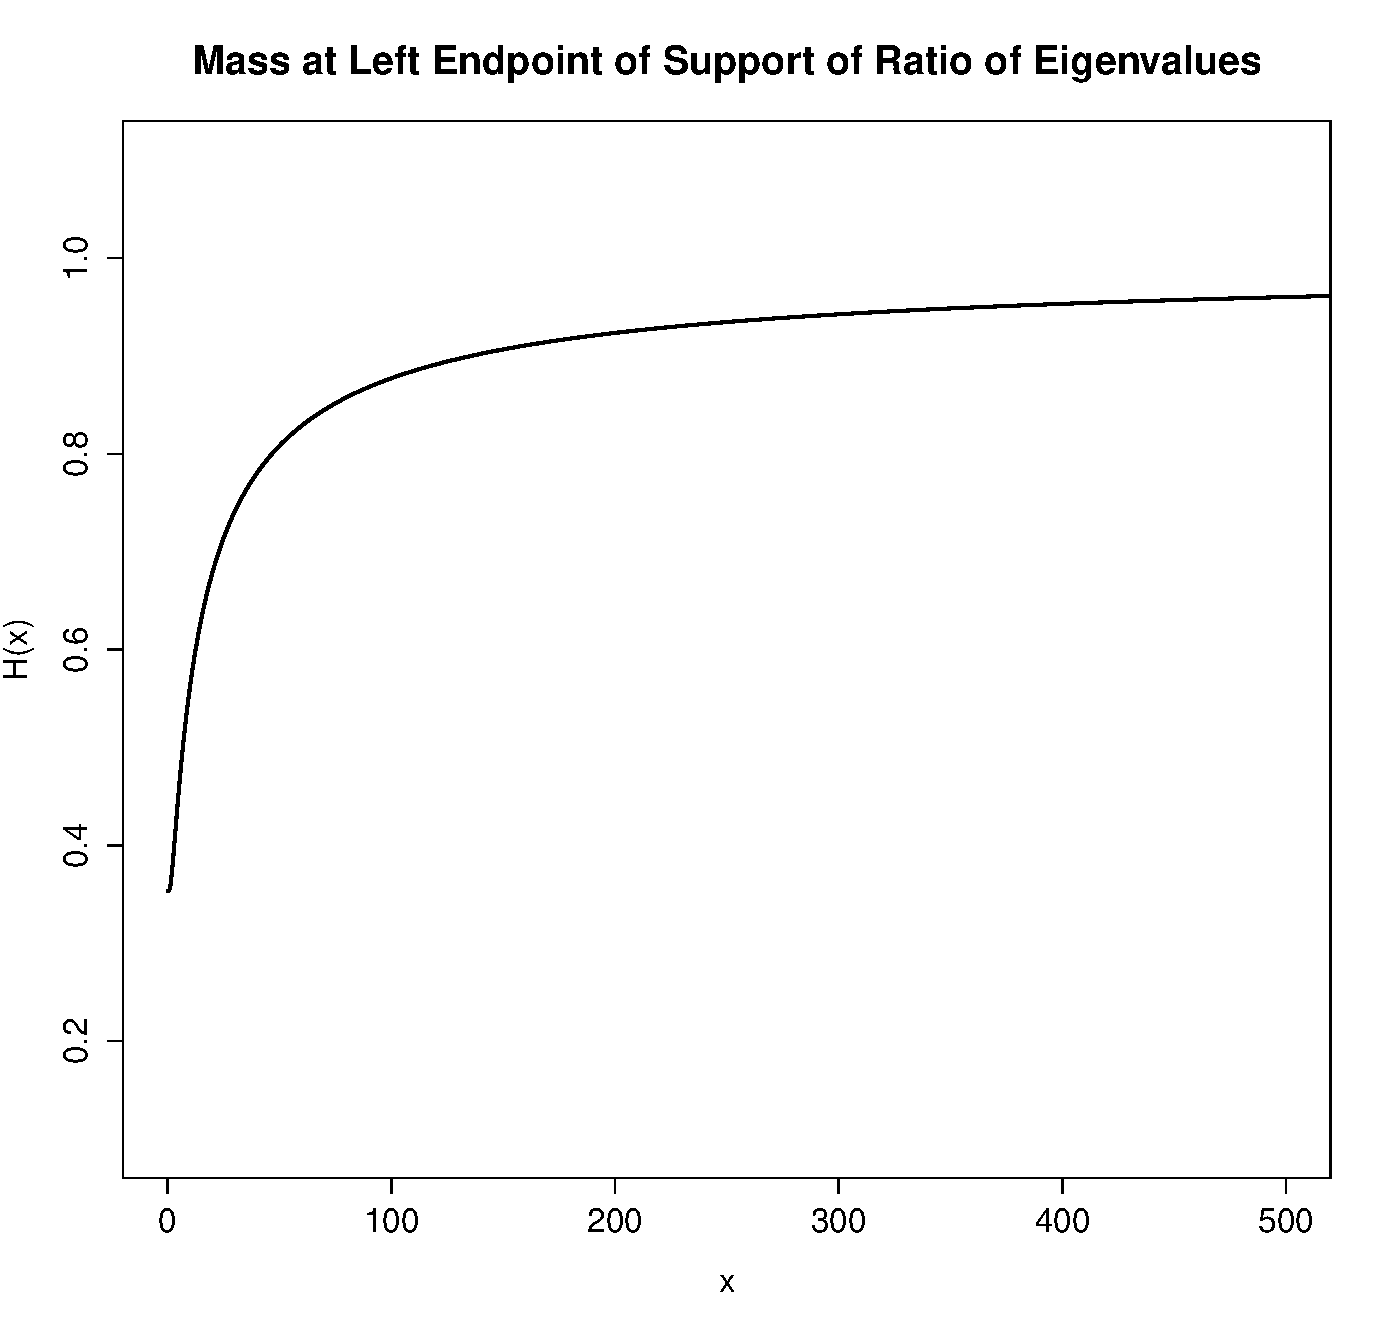
\includegraphics[scale=.35]{Hfunction.pdf}
\end{center}
\caption{Graph of $G(x)=\P(\Gamma_1/\Gamma_2\le2^{-\alpha}|\Gamma_1<(x/8)^{-\alpha/2})$ when $\alpha=1.5$.}
\label{fig:2}
\end{figure}
In addition, from Remark~\ref{rem:4.5}, we also have
\begin{equation*}
\dfrac{\la_{(1)}}{\la_1+\cdots +\la_p} \cid \dfrac{4}{5}\,
\dfrac{\Gamma_1^{-2/\alpha}}{\sum_{i=1}^\infty \Gamma_i^{-2/\alpha}}\,.
\end{equation*}
Clearly, the limit \rv\ is stochastically smaller than what one would get in the iid case; see \eqref{eq:limit}.
\end{example}
\begin{example}\label{exam:spectralgap}\rm
The previous example also illustrates the behavior of the two largest eigenvalues in the general case
when the rank $r$ of the matrix $\M$ is larger than one.
We have in general
\begin{equation*}
\dfrac{\lambda_{(2)}}{\lambda_{(1)}}\cid
\frac{v_2}{v_1}\,\1_{\{U<(v_2/v_1)^{\alpha/2}\}}+U^{2/\alpha}\,\1_{\{U\ge (v_2/v_1)^{\alpha/2}\}}\,.
\end{equation*}
In particular, the limiting
{\em self-normalized spectral gap} has \rep
\beao
\dfrac{\la_{(1)}-\la_{(2)}}{\la_{(1)}} \cid \dfrac{v_1-v_2}{v_1}\,\1_{\{U<(v_2/v_1)^{\alpha/2}\}}+(1-U^{2/\alpha})\,\1_{\{U\ge (v_2/v_1)^{\alpha/2}\}}\,.
\eeao
The limiting variable assumes values in $(0,1-v_2/v_1]$  and has an atom at the right end-point.
This is in contrast to the iid case
and to the case when $r=1$ (hence $v_2=0$) including the case of iid rows and the separable case; see Example~\ref{exam:separable}.
\end{example}
\begin{example}\label{exam:separable}
{\em We consider the separable case when  $h_{kl}=\theta_kc_l$, $k,l \in \Z$, where $(c_l)$, $(\theta_k)$ are
  real sequences such that the conditions on $(h_{kl})$ in
  Theorem~\ref{thm:mains} hold. In this case,
\begin{equation*}
\M= \sum_{l\in \Z} c_l^2\;\; (\theta_i\theta_j)_{i,j \in \Z}\,.
\end{equation*}
Note that $r=1$ with the only non-negative eigenvalue
\beao
v_1=\sum_{l\in \Z} c_l^2\;\;\sum_{k\in \Z}\theta_k^2\,.
\eeao
In this
case, the limiting point process in Theorem~\ref{cor:1} is a PRM on
$(0,\infty)$ with mean measure of $(y,\infty)$ given by $(v_1/
y)^{\alpha/2}$, $y>0$. The normalized eigenvalues have similar asymptotic behavior as
in the case of iid entries. For example, the log-spacings have the same limit as in the iid case for fixed $k$,
\beao
\big(\log \la_{(1)}-\log \la_{(2)},\ldots,\log \la_{(k+1)}-\log \la_{(k)}\big)\std
-\dfrac{2}{\alpha}\,\big(\log(\Gamma_1/\Gamma_2),\ldots,\log (\Gamma_{k}/\Gamma_{k+1})\big)\,.
\eeao
The same observation applies to the ratio of the largest eigenvalue and the trace in the case $\alpha\in (0,2)$:
\beao
\dfrac{\la_{(1)}}{{\rm tr} (\X \X')}=\dfrac{\la_{(1)}}{\la_1+\cdots +\la_p} \std
\dfrac{\Gamma_1^{-2/\alpha}}{\sum_{i=1}^\infty \Gamma_i^{-2/\alpha}}\,.
\eeao
We also mentioned in Example~\ref{exam:spectralgap} that the \ds al limit of the self-normalized spectral gap has no atom
as in the iid case.
}
\end{example}

\subsection{S\&P 500 data}\label{sec:sp500}
We conduct a short analysis of the largest eigenvalues of the univariate log-return time series which compose
the S\&P 500 stock index; see Section~\ref{subsec:1.2} for a description of the data.
Although there is strong empirical evidence that these univariate series have power-law tails
(see Figure~\ref{fig:SP500_tail_indices}) we  do not expect that they
have the same tail index. One way to proceed would be to ignore this fact because the tail indices are
in a close range and the differences are due to large sampling errors for estimating such quantities.  One could also collect \ts\ with similar
tail indices in the same group.
In this case, the dimension $p$ decreases. This grouping would be a rather arbitrary classification method.
We have chosen a third way: to use rank transforms.
This approach has its merits because it aims at standardizing the tails but it also has a major disadvantage: one destroys
the covariance structure underlying the data.
\par
Given a $p\times n$ matrix $(R_{it})_{i = 1, \cdots, p;t=1,\cdots, n}$,
we construct a matrix $\X$ via the rank transforms
\begin{equation*}
  X_{it} = -\Big[
    \log \Big(\frac{1}{n+1} \sum_{\tau=1}^n \1_{\{R_{i\tau} \leq R_{it}\}} \Big)
  \Big]^{-1} \,,\qquad i=1,\ldots,p;t=1,\ldots,n\,.
\end{equation*}
\begin{figure}[htb!]
  \centering
    \includegraphics[scale=0.550]{EigenRatioSP500_ranks_log_50_shown.pdf}
  \caption{The logarithms of the ratios $\lambda_{(i+1)} / \lambda_{(i)}$ for the S\&P 500 series after rank transform.
We also show the 1, 50 and 99\% quantiles (bottom, middle, top lines, respectively) of the variables
$\log((\Gamma_i/ \Gamma_{i+1})^{2})$. }
  \label{fig:EigenRatio}
\end{figure}
\begin{figure}[htb!]
  \centering
    \includegraphics[scale=0.550]{EigenRatioSP500_log_50_shown.pdf}
  \caption{The logarithms of the ratios $\lambda_{(i+1)} / \lambda_{(i)}$ for the original (non-rank transformed) S\&P 500 log-return data.
We also show the 1, 50 and 99\% quantiles (bottom, middle, top lines, respectively) of the variables
$\log((\Gamma_i/ \Gamma_{i+1})^{2/2.3})$; see also Figure~\ref{fig:EigenRatio} for comparison.}\label{fig:22}
\end{figure}

%\begin{figure}[htb!]
%  \centering
%    \includegraphics[scale=0.550]{EigenRatioSP500_lin2_250_shown.pdf}
%  \caption{{\green Same as Figure \ref{fig:EigenRatio} but on original scale, no logarithm. Choose one.}}
%\end{figure}

If the rows $R_{i1}, \ldots, R_{in}$ were iid (or, more generally, stationary ergodic)
with a continuous \ds\  then
the averages under the logarithm would be  asymptotically uniform
on $(0,1)$ as $n \to \infty$. Hence $X_{it}$ would  be \asy ally standard
Fr\'echet $\Phi_1$-distributed.
In what follows, we assume that the aforementioned univariate \ts\ of the S\&P 500 index have undergone the rank transform and that
their marginal \ds s are close to $\Phi_1$; we
always use the symbol $\X$ for the resulting multivariate series.
\par
In Figure~\ref{fig:EigenRatio} we show the ratios of the consecutive ordered eigenvalues $(\la_{(i+1)}/\la_{(i)})$
of the matrix $\X\X'$. This graph shows the rather surprising fact that the ratios are close to one even for small values $i$.
We also show the 1, 50 and 99 \% quantiles of the variables $((\Gamma_{i}/\Gamma_{i+1})^{2/\alpha})$ calculated from the formula
\beam\label{eq:iid}
\P\big((\Gamma_{i} /\Gamma_{i+1})^{2/\alpha}\le x \big) = x^{i \cdot \alpha/2}, \quad x\in (0,1)\,.
\eeam
For increasing $i$, the \ds\ is concentrated closely to 1, in agreement with the \slln\ which yields
$\Gamma_{i} /\Gamma_{i+1}\stas 1$ as $i\to\infty$.
The \asy\ \ds s \eqref{eq:iid} correspond to the case when the matrix
$\M$ has rank $r=1$. It includes the iid and separable cases;
see Example~\ref{exam:separable}. The shown \asy\ quantiles are in agreement with the rank $r=1$ hypothesis.
\par
For comparison, in Figure~\ref{fig:22} we also show the ratios  $(\la_{(i+1)}/\la_{(i)})$ for the 
non-rank transformed S\&P 500 data and the 1, 50 and 99\% quantiles of the variables
$\log((\Gamma_i/ \Gamma_{i+1})^{2/\alpha})$, where we choose $\alpha=2.3$ motivated by the estimated tail indices in 
Figure~\ref{fig:SP500_tail_indices}.
The two graphs in Figure~\ref{fig:EigenRatio} and Figure~\ref{fig:22} are quite similar but the smallest ratios for the original data are slightly larger than
for the rank-transformed data.




%--------------------------------------------------------------------------------------
\subsection{Sums of squares of sample autocovariance matrices}\label{sec:possemidef}
In this section we consider some additive \fct s
of the squares of $\A_n(s)=\X_n(0)\X_n(s)'$ given by $\A_n(s)\A_n(s)'$ for $s=0,1,\ldots$. By definition of the singular values of a matrix
(see  \eqref{eq:sigma}), the non-negative definite
matrix $\A_n(s)\A_n(s)'$ has eigenvalues $(\la_i^2(s))_{i=1,\ldots,p}$.
\par
The following result is a corollary of Theorem~\ref{thm:mains}.
\begin{proposition}\label{thm:mainstr} Consider the linear process \eqref{eq:1} under
the conditions of Theorem~\ref{thm:mains}. Then the following statements hold for $s\ge 0$:
\begin{enumerate}
\item[$(1)$]
We consider two disjoint cases:
$\alpha \in (0,2)$ and $\beta\in (0,\infty)$, or
$\alpha\in [2,4)$ and $\beta$ satisfying \ref{Cbeta}. Then
\beao
a_{np}^{-4} \max_{i=1,\ldots,p} |\lambda_{(i)}^2(s)-\delta_{(i)}^2(s)| \cip 0, \quad \nto.
\eeao
\item[$(2)$]
Assume $\beta\in [0,1]$.
If $\alpha \in (0,2]$, $\E[Z^2]=\infty$ or $\alpha\in [2,4)$, $\E [Z^2]<\infty$ and $\beta \in (\alpha/2-1,1]$, then
\beao
a_{np}^{-4} \max_{i=1,\ldots,p} |\la_{(i)}^2(s)-(\gamma_{(i)}^\rightarrow(s))^2| \cip 0, \quad \nto.
\eeao
Assume $\beta>1$. If $\alpha \in (0,2]$, $\E[Z^2]=\infty$ or $\alpha\in [2,4)$, $\E [Z^2]<\infty$ and $\beta^{-1} \in (\alpha/2-1,1]$. Then
\beao
a_{np}^{-4} \max_{i=1,\ldots,p} |\la_{(i)}^2(s)-(\gamma_{(i)}^\downarrow(s))^2| \cip 0, \quad \nto.
\eeao
\end{enumerate}
\end{proposition}
To the best of our knowledge, sums of squares of sample autocovariance matrices were used first in the paper by Lam and Yao
\cite{lam:yao}; their \ts\ model is quite different from ours.
\begin{proof}
Part (1).
The proof follows from Theorem~\ref{thm:mains} if we can show that
\beao
a_{np}^{-2}\max_{i=1,\ldots,p} \big(\la_{(i)}(s)+\delta_{(i)}(s) \big)=O_\P(1)\,\quad \nto\,.
\eeao
We have by Theorem~\ref{cor:1},
\beam \label{eq:gdfg}
a_{np}^{-2}\max_{i=1\ldots,p} \la_{(i)}(s)=a_{np}^{-2}\la_{(1)}(s) \cid c\, \xi_{\alpha/2}\,,
\eeam
where $\xi_{\alpha/2}$ has a $\Phi_{\alpha/2}$ \ds . In view of Theorem~\ref{thm:mains}(1) we also have
\beao
a_{np}^{-2}\max_{i=1\ldots,p} \delta_{(i)}(s)\cid c\, \xi_{\alpha/2}\,.
\eeao
Therefore, again using Theorem~\ref{thm:mains}(1), we have
\beao
\lefteqn{a_{np}^{-4} \max_{i=1,\ldots,p} |\lambda_{(i)}^2(s)-\delta_{(i)}^2(s)|}\\
&\le &\big[a_{np}^{-2} \max_{i=1,\ldots,p} |\lambda_{(i)}(s)-\delta_{(i)}(s)|\big]\,
\big[a_{np}^{-2} \max_{i=1,\ldots,p}\big ( |\lambda_{(i)}(s)|+|\delta_{(i)}(s)|\big)\big]
\cip 0, \quad \nto.
\eeao
This proves part (1).\\[1mm]
Part (2). Now assume $\beta\in [0,1]$ and $\alpha \in (0,2]$, $\E[Z^2]=\infty$ or $\alpha\in [2,4)$, $\E [Z^2]<\infty$ and $\beta\in (\alpha/2-1,1]$. Then \eqref{eq:gdfg} is still true and we have by Theorem~\ref{thm:mains}(2) and Theorem~\ref{cor:1}
\beao
a_{np}^{-2}\max_{i=1\ldots,p} \gamma_{(i)}^{\rightarrow}(s)\cid c\, \xi_{\alpha/2}\,.
\eeao
We then have
\beao
\lefteqn{a_{np}^{-4} \max_{i=1,\ldots,p} |\lambda_{(i)}^2(s)-(\gamma_{(i)}^\rightarrow(s))^2|}\\
&\le &\big[a_{np}^{-2} \max_{i=1,\ldots,p} |\lambda_{(i)}(s) -\gamma_{(i)}^\rightarrow(s)|\big]\,
\big[a_{np}^{-2} \max_{i=1,\ldots,p}\big ( \lambda_{(i)}(s)+\gamma_{(i)}^\rightarrow(s)
\big)\big]
\cip 0\,, \qquad \nto.
\eeao
The proof of the remaining part is similar and therefore omitted.
\end{proof}
Now, using Proposition~\ref{thm:mainstr} and a continuous mapping argument, we can show
limit theory for the eigenvalues
\beao
w_{(1)}(s_0,s_1)\ge \cdots \ge w_{(p)}(s_0,s_1)\,,\qquad 0\le s_0\le s_1\,,
\eeao
of the non-negative definite random matrices
\begin{equation}\label{eq:sumA}
\sum_{s=s_0}^{s_1} \A_n(s) \A_n(s)'\,.
\end{equation}

\begin{proposition}\label{prop:sumsmal}
Assume $0\le s_0\le s_1$ and the conditions of Theorem~\ref{thm:mains} hold.
If $\alpha \in (0,4)$ and $\beta\in (0,1] \cap  (\alpha/2-1,1]$ then
\begin{equation*}
a_{np}^{-4} \max_{i=1,\ldots,p} |w_{(i)}(s_0,s_1)-\omega_{(i)}(s_0,s_1)| \cip 0, \quad \nto,
\end{equation*}
where $\omega_{(i)}(s_0,s_1)$ are the ordered values of the set $\{Z_{(i),np}^4 v_j(s_0,s_1), i=1,\ldots,p;j=1,2,\ldots\}$
and $(v_j(s_0,s_1))$ are the ordered eigenvalues of $ \sum_{s=s_0}^{s_1} \M(s)\M(s)'$.
\end{proposition}


\begin{example}\label{exam:additive}{\em
\begin{figure}[htb!]
  \centering
  \subfigure[]
{
    \includegraphics[scale=0.4]{eigen_sum.pdf}
    \label{fig:LamYao:a}
  }
  \subfigure[] {
    \includegraphics[scale=0.375]{eigen_sum_ratio.pdf}
    \label{fig:LamYao:b}
  }
  \caption{The largest eigenvalues of the sums of the squared autocovariance
    matrices compared with the sums of the largest eigenvalues of these matrices
    for the S\&P 500 data for different values $s_1$. The two values are surprisingly close to each other; mind the scale
of the $y$-axis. We also show their ratios.}
  \label{fig:LamYao}
\end{figure}
Recall the separable case from Example~\ref{exam:separable}, i.e.,
$h_{kl}=\theta_kc_l$, $k,l \ge 0$, where $(c_l)$, $(\theta_k)$ are
real sequences such that the conditions on $(h_{kl})$ in
Theorem~\ref{thm:mains} hold.
%Let $\alpha \in (0,2)$ and set
%\begin{equation*}
%\theta = (\theta_0, \theta_1,\theta_2,\ldots)' \quad \mbox{and} \quad
%c= (c_0,c_1,c_2, \ldots)'.
%\end{equation*}
Write $\Theta_{ij}=\theta_i \theta_j$. It is symmetric and has rank one; the only non-zero
eigenvalue is $\gamma_\theta(0)=\sum_{k=0}^\infty \theta_k^2$. Hence $\Theta$  is non-negative definite.
We get from \eqref{eq:m} that
\begin{equation*}
\M(s)=\gamma_c(s)\, \Theta, \quad s\ge 0\,,
\end{equation*}
where
\beao
\gamma_c(s)=\sum_{l=0}^\infty c_lc_{l+s}\,,\qquad s\ge 0\,.
\eeao
The matrix $\M(s)$ has the only non-zero eigenvalue $\gamma_c(s)\gamma_\theta(0)$.
The factors $(\gamma_c(s))$ can be positive or negative; they constitute the autocovariance \fct\ of a stationary linear process
with coefficients $(c_l)$.
Accordingly, $\M(s)$ is either non-negative or non-positive definite. %This explains why a symmetrization of $\M(s)$ is irrelevant.
Now we consider the non-negative definite matrix
\beao
\sum_{s=s_0}^{s_1} \M(s)\,\M(s)'= \sum_{s=s_0}^{s_1}\gamma_c^2(s)\,\Theta\Theta'\,.
\eeao
This matrix has rank $1$ and its largest eigenvalue is given by
\begin{equation*}
C_{c,\theta}(s_0,s_1)=\sum_{s=s_0}^{s_1}\gamma_c^2(s)\,\gamma_\theta^2(0)\,.
\end{equation*}
An application of
Proposition~\ref{prop:sumsmal} yields that the ordered eigenvalues of $a_{np}^{-4}\sum_{s=s_0}^{s_1}\A_n(s)\A_n(s)'$
are uniformly approximated by the quantities
\begin{equation}\label{eq:drtgdfg}
a_{np}^{-4} Z_{(i),np}^4 C_{c,\theta}(s_0,s_1)\,,\qquad  i=1,\ldots,p\,.
\end{equation}
Since
\beao
C_{c,\theta}(s_0,s_1)= \sum_{i=s_0}^{s_1} C_{c,\theta}(i,i)
\eeao
one gets the remarkable property that
\beao
&&a_{np}^{-4}\max_{i=1,\ldots,p} \Big| \la_{(i)}\Big(\sum_{s=s_0}^{s_1}\A_n(s)\A_n(s)'\Big)- Z_{(i),np}^4 C_{c,\theta}(s_0,s_1)\Big|\\
&=&a_{np}^{-4}\max_{i=1,\ldots,p} \Big|\sum_{s=s_0}^{s_1}\la_{(i)}(\A_n(s)\A_n(s)')- Z_{(i),np}^4 C_{c,\theta}(s_0,s_1)\Big|+o_P(1)\,.
\eeao
In particular, for $s_1\ge s_0$ we get the weak \con\ of the \pp es towards a PRM:
\beao
\sum_{i=1}^p \varepsilon_{a_{np}^{-4}\Big(\la_{i}\Big(\sum_{s=s_0}^{s_0}\A_n(s)\A_n(s)'\big)\,,\ldots,\la_{i}\big(\sum_{s=s_0}^{s_1}\A_n(s)\A_n(s)'\big)\Big)}
\std \sum_{i=1}^\infty \varepsilon_{\Gamma_i^{-4/\alpha} \Big(C_{c,\theta}(s_0,s_0),\ldots,C_{c,\theta}(s_0,s_1)\Big)}\,.
\eeao

}
\end{example}
\begin{example}\em
In Figure~\ref{fig:LamYao} we calculate the largest eigenvalues
$\la_{(1)}\big(\sum_{s=0}^{s_1}\A_n(s)\A_n(s)'\big)$ for $s_1=0,\ldots,5$ as well as the sums of the largest eigenvalues
$\sum_{s=0}^{s_1}\la_{(1)}\big(\A_n(s)\A_n(s)'\big)$
the log-return series from the S\&P 500 index described in Section~\ref{subsec:1.2}. The data are not rank-transformed.
We notice that
the two values are surprisingly close across the values $s_0=0,\ldots,5$. This phenomenon
could be explained by the structure of the eigenvalues in Example~\ref{exam:additive}.
Also note that the largest eigenvalue $\A_n(0)\A_n(0)'$ makes a major contribution to the values in Figure~\ref{fig:LamYao};
the contribution of the squares $\A_n(s)\A_n(s)'$, $s=1,\ldots,5,$ to the largest eigenvalue of the sum of squares is less substantial.
%Figure~\ref{fig:LamYao}(b) shows the same calculations for the matrices studied in Example~\ref{exam:4.6cont}. Here cancellation is possible (see \eqref{eq:Xrgsdf}) which is indicated by the fact that the red line does not follow the blue line as well as in (a).
\end{example}
%\section{\red Some conclusions?}\setcounter{equation}{0}
%{\em Say something about EVT and largest eigenvalues}


\ifx\phdthesis\undefined
\appendix
\else
\begin{subappendices}
\fi


\section{Auxiliary results}\label{appendix:A}\setcounter{equation}{0}

Let $(Z_i)$ be iid copies of $Z$ whose distribution satisfies
\begin{equation*}
\P(Z>x)\sim p_+ \dfrac{L(x)}{x^{\alpha}}\quad\mbox{and}\quad  \P(Z\le -x)\sim p_-
\dfrac{L(x)}{x^{\alpha}} \,,\quad \xto\,,
\end{equation*}
 for some tail index $\alpha>0$,
where $p_+,p_-\ge 0$ with $p_++p_-=1$ and $L$ is a slowly varying function. If $\E[|Z|]<\infty$ also assume $\E[Z]=0$. The product $Z_1Z_2$ is regular varying with the same index $\alpha$ and $\P(|Z_1Z_2|>x)= x^{-\alpha} L_1(x)$, where $L_1$ is slowly varying function different from $L$;
see Embrechts and Goldie \cite{embrechts:goldie:1980}.
Write
\begin{equation*}
S_n=Z_1+\cdots +Z_n\,,\quad n\ge 1,
\end{equation*} and consider a sequence $(a_n)$ such that $\P(|Z|>a_n)\sim n^{-1}$.

\subsection{Large deviation results}
The following theorem can be found in
Nagaev \cite{nagaev:1979} and Cline and Hsing
\cite{cline:hsing:1998} for $\alpha>2$ and $\alpha\le 2$,
respectively; see also  Denisov et al.~\cite{denisov:dieker:shneer:2008}.
\begin{theorem}\label{thm:nagaev}
Under the assumptions on the iid sequence $(Z_t)$
given above the following relation holds
\begin{equation*}
\sup_{x\ge c_n}\left|\dfrac{\P(S_n>x )}{n\P(|Z|>x)} -p_+ \right|\to 0\,,
\end{equation*}
where $(c_n)$ is any sequence satisfying $c_n/a_n\to  \infty$ for
$\alpha\le 2$ and $c_n\ge \sqrt{(\alpha-2)n\log n}$ for $\alpha>2$.
\end{theorem}




\subsection{A point process convergence result}
Assume that the conditions at the beginning of Appendix \ref{appendix:A} hold.
Consider a sequence of iid copies $(S_{n}^{(t)})_{t=1,2,\ldots}$
of $S_n$ and the sequence of point processes
\begin{equation*}
N_n= \sum_{t=1}^{p} \vep_{a_{np}^{-1} S_{n}^{(t)}}, \quad n=1,2,\ldots\,,
\end{equation*}
for an integer sequence $p=p_n\to\infty$. We assume that the state space of the
point processes $N_n$ is $\overline{\R}_0=[\R\cup\{\pm \infty\}]\backslash \{0\}$.
\begin{lemma}\label{lem:ppr}
Assume $\alpha \in (0,2)$ and the
conditions of  Appendix~\ref{appendix:A}
on the iid sequence $(Z_t)$ and the normalizing sequence $(a_n)$. Then the limit relation
$N_n\cid N$ holds in the space of point measures on $\overline{\R}_0$
equipped with the vague topology (see
\cite{resnick:1987,resnick:2007})
for a  Poisson random measure $N$ with state space $\overline{\R}_0$ and intensity measure $\mu_\alpha(dx)=\alpha |x|^{-\alpha-1} (p_+ \1_{\{x>0\}}+ p_- \1_{\{x<0\}}) dx$.
\end{lemma}
\begin{proof}
According to Resnick \cite{resnick:1987}, Proposition 3.21, we need to
show that
$p\, \P(a_{np}^{-1}S_n\in \cdot)\civ \mu_\alpha
$,
where $\civ$ denotes vague convergence of Radon measures on  $\overline{\R}_0$.
Observe that we have $a_{np}/a_n\to\infty$ as $\nto$. This fact and
$\alpha\in (0,2)$ allow one to apply
Theorem~\ref{thm:nagaev}:
\begin{equation*}
\dfrac{\P( S_n >x a_{np})}{n\,\P(|Z|>  a_{np})}\to p_+ x^{-\alpha}
\quad \mbox{and}\quad \dfrac{\P( S_n \le -x a_{np})}{n\,\P(|Z|>
  a_{np})}\to p_-\, x^{-\alpha}\,,\quad x>0\,.
\end{equation*}
On the other hand, $n\,\P(|Z|>  a_{np})\sim p^{-1}$ as $\nto$.
This proves the lemma.
\end{proof}

\ifx\phdthesis\undefined
\else
\end{subappendices}
\fi


%correlation Chapter
\chapter[Almost sure convergence of the largest and smallest eigenvalues of high-dimensional sample correlation matrices under infinite fourth moment]{{\huge Almost sure convergence of the largest and smallest eigenvalues of high-dimensional sample correlation matrices under infinite fourth moment}}\label{ch:corr}
\chaptermark{Extreme eigenvalues of sample correlation matrices}


\begin{center}
\textsc{Johannes Heiny \& Thomas Mikosch (2016)}
\end{center}

\begin{abstract}{In this paper, we show that the largest and smallest eigenvalues 
of a sample correlation matrix stemming from $n$ independent observations of a $p$-dimensional 
time series with iid components converge almost surely to $(1+\sqrt{\gamma})^2$ and $(1-\sqrt{\gamma})^2$, 
respectively, as $\nto$, if $p/n\to \gamma \in (0,1]$ and the truncated variance of the entry 
distribution is ``almost slowly varying'', a condition we describe via moment 
properties of self-normalized sums. Moreover, the empirical spectral distributions 
of these sample correlation matrices converge weakly, with probability $1$, to the \MP law, 
which extends a result in \cite{bai:zhou:2008}. We compare the behavior of the eigenvalues of the 
sample covariance and sample correlation matrices and argue that the latter seems more robust, 
in particular in the case of infinite fourth moment. We briefly address some practical issues 
for the estimation of extreme eigenvalues in a simulation study.   
\par
In our proofs we use the method of moments combined with a Path-Shortening Algorithm, 
which efficiently uses the structure of sample correlation matrices, 
to calculate precise bounds for matrix norms. We believe that this new approach could be of further use in random matrix theory. 
\medskip

\noindent {\bf Keywords:} Sample correlation matrix, infinite fourth moment, largest eigenvalue, smallest eigenvalue, 
spectral distribution, sample covariance matrix, self-normalization, regular variation, combinatorics.}
\end{abstract}

\newpage
\section{Introduction and notation}\label{sec:sdlgj}

%{\red Discuss $p/n \to 0$.} 
%{\blue Inconsistent use of referenes, sometimes with or without names. I cannot see a general rule.}
In modern statistical analyses one is often faced with large data sets where both the dimension of the observations and the sample size are large. The dramatic increase and improvement of computing power and data collection devices have triggered the necessity to study and interpret the sometimes overwhelming amounts of data in an efficient and tractable way. Huge data sets arise naturally in wireless communication, finance, natural sciences and genetic engineering.
For such data one commonly studies the dependence structure via covariances and correlations which can be estimated by their sample analogs. {\em Principal component analysis}, for example, uses an orthogonal transformation of the data such that only a few of the resulting vectors explain most of the variation in the data. The empirical variances of these so-called {\em principal component vectors} are the largest eigenvalues of the {\em sample covariance or correlation matrix}.  

Throughout this paper we consider the $p\times n$ data matrix
\begin{equation*}
\X=\X_n=(X_{it})_{i=1,\ldots,p; t=1,\ldots,n}
\end{equation*}
of identically distributed entries $(X_{it})$ with generic element $X$, where we assume $\E[X]=0$ and $\E[X^2]=1$ if the first and second moments of $X$ are finite, respectively. A column of $\X$ represents an observation of a $p$-dimensional time series. 

Random matrix theory provides a great variety of results on the ordered eigenvalues
\begin{equation}\label{eq:deflambda}
\la_{(1)} \ge \cdots \ge\la_{(p)}\,,
\end{equation}
of the (non-normalized) {\em sample covariance matrix} $\X\X'$. Here we will only discuss the case $p=p_n \to \infty$ and, unless stated otherwise, we assume the growth condition  
\begin{equation}\label{Cpn}
\lim_{\nto} \frac{p_n}{n}\to \gamma\in (0,1]\,. \tag{$G_{\gamma}$}
\end{equation} 
For the finite $p$ case, we refer to \cite{anderson:1963,muirhead,janssen:mikosch:rezapour:xie:2016}.
When studying the asymptotic properties of estimators under \eqref{Cpn}
one often obtains results that dramatically differ from the standard $p$ fixed, $\nto$ case, in which the spectrum of $(n^{-1}\X\X')$ converges to its population covariance spectrum. In 1967, Mar\v cenko and Pastur \cite{marchenko:pastur:1967} observed that even in the case of iid entries $(X_{it})$ with $\E[X^2]=1$ the eigenvalues $(\lambda_{(i)}/n)$ do not concentrate around $1$. For more examples, see \cite[Chapter 1]{bai:silverstein:2010} and \cite{elkaroui:2009}. Typical applications where \eqref{Cpn} seems reasonable are discussed in \cite{johnstone:2001,donoho:2000}. 
\par

In comparison with $(\lambda_{(i)})$, much less is known about the ordered eigenvalues
\begin{equation*}
\mu_{(1)} \ge \cdots \ge\mu_{(p)}\,
\end{equation*} 
of the {\em sample correlation matrix} $\bfR=\Y\Y'$ with entries
\begin{equation}\label{eq:corrR}
R_{ij}=\sum_{t=1}^n \frac{X_{it}X_{jt}}{\sqrt{D_i} \sqrt{D_j}} = \sum_{t=1}^n Y_{it}Y_{jt}\,, \quad i,j=1,\ldots,p\,.
\end{equation}
In this paper we will often make use of the notation $\Y=(Y_{it})=(X_{it}/\sqrt{D_i})$ and
\begin{equation}\label{eq:D}
D_i=D_i^{(n)}=\sum_{t=1}^n X_{it}^2\,, \qquad
i=1,\ldots,p;\;  n\ge 1\,.
\end{equation} 
Note that the dependence of $(\lambda_{(i)})$ and $(\mu_{(i)})$ on $n$ is suppressed in the notation.


%---------------------------------------------------------------------------------------
\subsection{The case $(X_{it})$ iid, $\E[X^4]<\infty$ and $\E[X^2]=1$}  

In this case the behavior of the eigenvalues of the sample covariance matrix $\X\X'$ and the sample correlation matrix $\bfR$ are closely intertwined. 
\par 

For any random $p\times p$ matrix $\bfA$ with real eigenvalues $\lambda_1(\bfA),\ldots,\lambda_p(\bfA)$ the {\em empirical spectral distribution} is defined by 
\begin{equation*}
F_{\bfA}(x)= \frac{1}{p}\; \sum_{i=1}^p \1_{\{ \lambda_i(\bfA)\le x \}}, \qquad x\in  \R\,.
\end{equation*}
Many functionals of the eigenvalues $\lambda_1(\bfA),\ldots,\lambda_p(\bfA)$ can be expressed in terms of $F_{\bfA}$ \cite{bai:fang:liang:2014}, for instance
\begin{equation*}
\det \bfA = \prod_{i=1}^p \lambda_i(\bfA) = \exp \Big( p \int_{0}^{\infty} \log x \;\dint F_{\bfA}(x) \Big)\,.
\end{equation*}
A major problem in random matrix theory is to find the weak limit of $(F_{\bfA_n})$ for suitable sequences $(\bfA_n)$; see for example \cite{bai:silverstein:2010,yao:zheng:bai:2015} for more details. By weak convergence of a sequence of probability distributions $(F_{\bfA_n})$ 
to a \pro y \ds\ $F$, we mean $\lim_{\nto} F_{\bfA_n}(x)=F(x) \,\as$ for all continuity points of $F$.
In this context a useful tool is the {\em Stieltjes transform}
of the empirical spectral distribution $F_{\bfA}$:
\begin{equation*}
s_{\bfA}(z)= \int_{\R} \frac{1}{x-z} \dint F_{\bfA}(x) = \frac{1}{p} \tr(\bfA -z \bfI)^{-1}\,, \quad z\in \C^+\,,
\end{equation*}
where $\C^+$ denotes the complex numbers with positive imaginary part. 
Weak convergence of $(F_{\bfA_n})$ to $F$ is equivalent to $s_{F_{\bfA_n}}(z) \to s_F(z)$ a.s. for all $z\in \C^+$.

Under the growth condition \eqref{Cpn}, the sequence of empirical spectral distributions of the normalized sample covariance matrix $n^{-1} \X\X'$ converges weakly to the \MP law with density
\begin{eqnarray}\label{eq:MPch4}
f_\gamma(x) = 
\left\{\begin{array}{cc}
\frac{1}{2\pi x\gamma} \sqrt{(b-x)(x-a)} \,, & \mbox{if } a\le x \le b, \\
 0 \,, & \mbox{otherwise,}
\end{array}\right.
\end{eqnarray}\noindent
where $\gamma\in (0,1]$, $a=(1 -\sqrt{\gamma})^2$ and $b=(1 +\sqrt{\gamma})^2$. This classical result is sometimes referred to as \MP theorem \cite{marchenko:pastur:1967}. Informally, the histogram of $(\lambda_{(i)}/n)$ is asymptotically non-random and the limiting shape depends only on the fraction $p/n$. For an illustration, see Figure~\ref{fig:alpha6}.
\par

The \MP law has $k$-th moment
\begin{equation}\label{eq:momentsmp}
\beta_k=\beta_k(\gamma)=\int_a^b x^k f_\gamma(x) \dint x=\sum_{r=1}^{k} \frac{1}{r} \binom{k}{r-1}\binom{k-1}{r-1}\gamma^{r-1}\,,\quad k\ge 1\,,
\end{equation}
and Stieltjes transform 
\beam\label{eq:stieltjestransform}
s(z)
=\int_{\R} \frac{1}{x-z}f_\gamma(x) \dint x 
= \frac{1-\gamma -z +\sqrt{(1+\gamma-z)^2-4\gamma}}{2 \gamma z} \,;
%+ \frac{1-\gamma}{\gamma z} \1_{\{\gamma>1\}}\,.
\eeam
see \cite[Chapter~3]{bai:silverstein:2010} or \cite{bai:fang:liang:2014,yao:zheng:bai:2015}.
\par

The \as~behavior of the extreme eigenvalues is more involved and therefore it has received significant attention in the literature. From the \MP theorem one can infer
\begin{equation}\label{eq:efsdf}
\limsup_{\nto} n^{-1}\lambda_{(p)} \le (1-\sqrt{\gamma})^2 \le (1+\sqrt{\gamma})^2 \le \liminf_{\nto} n^{-1}\lambda_{(1)}\, \quad \as
\end{equation}
The finiteness of the fourth moment of $X$ is necessary for the almost sure convergence of  $\lambda_{(1)}/n$; see \cite{baisilv}.
If $\E[X^4]<\infty$, one has (see \cite{bai:silverstein:2010}) 
\begin{equation}\label{eq:drtgdrghdr}
n^{-1} \la_{(1)} \to (1+\sqrt{\gamma})^2\, \quad \text{ and } \quad n^{-1} \la_{(p)} \to (1-\sqrt{\gamma})^2\, \quad \as
\end{equation}
\par

The minimal moment requirement for the convergence of the normalized smallest eigenvalue, however, was an open question for a long time.
Recently, it was proved in \cite{tikhomirov:2015} that $n^{-1} \la_{(p)} \to (1-\sqrt{\gamma})^2\, \as$ only requires a finite second moment.
Under suitable moment assumptions $\la_{(1)}$ and $\la_{(p)}$ possess {\em Tracy--Widom} fluctuations around their almost sure limits. For instance, 
the paper \cite{johnstone:2001} complemented \eqref{eq:drtgdrghdr} by the corresponding \clt\ in the special case of iid standard normal 
entries:
\beam\label{eq:tcch4}
 n^{2/3}\,\dfrac{(\sqrt{\gamma})^{1/3}}{\big(1+\sqrt{\gamma}\big)^{4/3}}\Big(\dfrac {\la_{(1)}}{n} -
\big(1+\sqrt{\tfrac pn }\big)^2\Big)
\std \xi\,,
\eeam
where the limiting \rv\ has a {\em Tracy--Widom \ds} of order 1. Notice that the centering
$\big(1+\sqrt{\tfrac pn }\big)^2$ can in general not be replaced by $(1+\sqrt{\gamma})^2$.
This \ds\ is ubiquitous in random matrix theory.
%It is defined via some ordinary differential equation; we refer to \cite{tracy:widom:2012} for a definition and properties.
Its distribution function $F_1$ is given by
\begin{equation*}
F_1(s) = \exp\Big\{
  -\frac{1}{2} \int_{s}^\infty [
    q(x) + (x - s) q^2(x)
 ] \dint x
\Big\}\,,
\end{equation*}
where $q(x)$ is the unique solution to the Painlev\'e II differential
equation
\begin{equation*}
  q''(x) = xq(x) + 2 q^3(x)\,,
\end{equation*}
where $ q(x)\sim {\rm Ai}(x)$ as $x \to \infty$ and Ai$(\cdot)$ is the Airy kernel; see Tracy and Widom~\cite{tracy:widom:2012} for details.
%We notice that the rate $n^{2/3}$ compares favorably to the $\sqrt{n}$-rate in the classical \clt\ for sums of iid finite variance \rv s.
\par

Sometimes practitioners would like to know ``to which extent the random matrix results would hold if one were concerned with sample correlation matrices and not sample covariance matrices \cite{elkaroui:2009}''.
A partial answer is that the aforementioned results also hold for the sample correlation matrix $\bfR$ and its eigenvalues $\mu_{(1)}\ge\cdots \ge \mu_{(p)}$. 
%The results on sample covariance matrices can be used to draw conclusions about the behavior of the eigenvalues of the sample correlation matrix.
With $\bfF= \diag (1/D_1,\ldots,1/D_p)$, we have $\bfR={\bfF}^{1/2} {\X}{\X}'{\bfF}^{1/2}$ which has the same eigenvalues as ${\X}{\X}'{\bfF}$. Weyl's inequality (see \cite{bhatia:1997}) yields
\begin{equation}\label{eq:lamu}
\begin{split}
\max_{i=1,\ldots,p} |\mu_{(i)}- n^{-1} \la_{(i)}| &\le \twonorm{{\X}{\X}'{\bfF}-n^{-1}{\X}{\X}' }\\
&\le n^{-1} \twonorm{{\X}{\X}'}  \twonorm{n \bfF- \bfI}\\
&= n^{-1} \la_{(1)} \max_{i=1,\ldots,p} \Big| \frac{n}{D_i} -1 \Big|\,,
\end{split}
\end{equation}
where for any matrix $\bfA$, $\twonorm{\bfA}$ denotes its spectral norm, i.e., its largest singular value.

Lemma 2 in \cite{bai:yin:1993} implies that $\E[X^4]<\infty$ is equivalent to
\begin{equation*}
\max_{i=1,\ldots,p} \Big| \frac{n}{D_i} -1 \Big| \cas 0\,,
\end{equation*}
while $n^{-1} \la_{(1)}\to (1+\sqrt{\gamma})^2~ \as$ Hence, $\max_{i=1,\ldots,p} |\mu_{(i)}- n^{-1} \la_{(i)}| \to 0~ \as$
This approach was used in \cite{jiang:2004,xiao:zhou:2010} to derive 
\begin{equation}\label{eq:drtgdrghdr1}
\mu_{(1)} \to (1+\sqrt{\gamma})^2\, \quad \text{ and } \quad  \mu_{(p)} \to (1-\sqrt{\gamma})^2\, \quad \as
\end{equation}
%Note that due to self-normalization of the sample correlation matrix we do not have to require $\E[X^2]=1$ which was needed for \eqref{eq:drtgdrghdr}. If $\E[X^2]\neq 1$, \eqref{eq:drtgdrghdr} would have to be adjusted to
%\begin{equation*}
%n^{-1} \la_{(1)} \to (1+\sqrt{\gamma})^2\E[X^2]\, \quad \text{ and } \quad n^{-1} \la_{(p)} \to (1-\sqrt{\gamma})^2\E[X^2]\, \quad \as
%\end{equation*}
If the assumption $\E[X^4]<\infty$ is weakened to $\lim_{\nto} n\,\P(X^4> n)=0$, the paper \cite{bai:yin:1993} proves that $n^{-1} \la_{(1)}\cip (1+\sqrt{\gamma})^2$ and $\max_{i=1,\ldots,p} \big| n/D_i -1 \big| \cip 0$. As a consequence, the limit results for $\mu_{(1)}$ and $\mu_{(p)}$ hold in probability instead of \as
\par
Distributional limit results have been derived for the appropriately centered and normalized eigenvalues of sample correlation matrices. The authors of \cite{bao:pan:zhou:2012} assumed iid, symmetric entries $X_{it}$ and that there exist positive constants $C,C'$ such that $\P(|X|\ge t^C)\le \e^{-t}, t\ge C'$. They showed \eqref{eq:tcch4} with $\lambda_{(1)}/n$ replaced by $\mu_{(1)}$.
%\beao
%n^{2/3}\,\dfrac{(\sqrt{\gamma})^{1/3}}{\big(1+\sqrt{\gamma}\big)^{4/3}}\Big(\mu_{(1)} -
%\big(1+\sqrt{\tfrac pn }\big)^2\Big)
%\std \xi\,,
%\eeao
A similar limit result holds for $\mu_{(p)}$.

\subsection{The case $(X_{it})$ iid and $\E[X^4]=\infty$}

Asymptotic theory for the eigenvalues of $\X\X'$ in the case of an entry distribution with infinite fourth moment was studied in \cite{soshnikov:2004,soshnikov:2006,auffinger:arous:peche:2009} in the cases when $p/n\to \gamma \in (0,\infty)$, while the authors of \cite{davis:mikosch:heiny:xie:2015,heiny:mikosch:2015:iid} allowed nearly arbitrary growth of the dimension $p$. 
In their model, the entries of $\X$ are regularly varying with index $\alpha>0$, implying that
\begin{equation}\label{eq:reg}
\P(|X|>x) = x^{-\alpha} L(x)\,,
\end{equation}
for a slowly varying function $L$. For $\alpha \in (0,4)$,  which implies an infinite fourth moment, they showed that $(a_{np}^{-2} \la_{(1)})$ converges to a \Frechet distributed random variable $\eta_{\alpha/2}$ with parameter $\alpha/2$ while $a_{np}^{-2} \la_{(p)}\cip 0$. Here the normalizing sequence $(a_n)$  is defined via $\P(|X|>a_n)\sim n^{-1}$, hence $n/a_{np}^{2}\to 0$. 

%If $\gamma=1$, the sample covariance matrix is almost surely singular. 
To illustrate the stark contrast between the cases $\alpha>4$ and $\alpha<4$, assume \eqref{Cpn} and $\E[X]=0$ if $\E[|X|]<\infty$. Then it follows from \eqref{eq:drtgdrghdr} that
\begin{equation}\label{eq:forch1}
\begin{split}
\frac{\la_{(p)}}{\la_{(1)}} &\cas \frac{(1-\sqrt{\gamma})^2}{(1+\sqrt{\gamma})^2} \quad \text{ if } \alpha >4\,,\\
\frac{a_{np}^2}{n} \frac{\la_{(p)}}{\la_{(1)}} &\cid \frac{(1-\sqrt{\gamma})^2}{\eta_{\alpha/2}} \quad \text{ if } \alpha \in (2,4)\,,\\
\frac{a_{np}^2}{n} \frac{\la_{(p)}}{\la_{(1)}} &\cas 0 \quad \text{ if } \alpha \in (0,2)\,,
\end{split}
\end{equation}
where the rate $a_{np}^2/n\to \infty$ in the last line can even be increased. 
To the best of our knowledge, a suitable normalization $(b_n)$ such that $(b_n \lambda_{(p)})$ has a nontrivial limit is not available when $ \alpha \in (0,2)$. 

Under \eqref{Cpn} the asymptotic behavior of the eigenvalues of sample correlation matrices can be very different from that of sample covariance matrices, especially for an entry distribution with infinite fourth moment. If $\alpha\in (2,4)$, the \MP theorem and Theorem 2.3 in \cite{bai:zhou:2008} assert that $(F_{n^{-1}\X\X'})$ and $(F_{\bfR})$  converge weakly to the \MP law. From \cite{baisilv} it is known that $\limsup_n \lambda_{(1)}/n =\infty \,\as$ 
\par

For $\E[X^4]=\infty$, the approach to sample correlation matrices from \eqref{eq:lamu} fails. No limit results for $\mu_{(1)}$ or $\mu_{(p)}$ seem to be available in the literature at this point, although Theorem 2.3 in \cite{bai:zhou:2008} ensures the weak convergence of the empirical spectral distribution $F_{\bfR}$ to the \MP law if $X$ is in the domain of attraction of the normal distribution. Analogously to \eqref{eq:efsdf}, the weak limit of $(F_{\bfR})$ provides a first idea what the limits of the extreme eigenvalues might be. 

\subsection{$(X_{it})$ identically distributed, but dependent}
For practical purposes it is important to work with arbitrary population covariance matrices and not just $n^{-1} \E[\X\X']=\bfI$. Based on well understood results in the iid case, numerous generalizations and estimation techniques have been developed. For many models the limiting spectral distribution can only be characterized in terms of an integral equation (=\MP equation) for its Stieltjes transform. Explicit solutions are more involved; see the monographs \cite{bai:silverstein:2010,bai:fang:liang:2014,yao:zheng:bai:2015}. Over the last couple of years siginificant progress on limiting spectral distributions for dependent time series was achieved; see for example %by Banna, Merlev{\`e}de and Peligrad 
\cite{banna:merlevede:peligrad:2015,banna:merlevede:2015,banna:2016}.
Since the sample covariance matrix is a poor estimator for the population covariance matrix in high dimension, a different approach to the fundamental problem of estimating population eigenvalues is needed. In \cite{elkaroui:purdom:2016} the authors find that the bootstrap works for the top eigenvalues if they are sufficiently separated from the bulk. Among others, El Karoui \cite{elkaroui:2008} proposed to use the \MP equation, which basically requires more insight into the empirical spectral distribution and its support. This was achieved in \cite{dobriban:2015}, where an algorithm for calculating the spectral distribution based on certain approximate integral equations for its Stieltjes transform was presented.

In view of \cite{davis:pfaffel:stelzer:2014,davis:mikosch:pfaffel:2015,davis:mikosch:heiny:xie:2015} the behavior of the top eigenvalues is reasonably well understood in the case of linear dependence among the $X_{it}$ and $\E[X^4]=\infty$. 
If $\E[X^4]<\infty$, similar arguments to \eqref{eq:lamu} can be developed to show that methods for sample covariance matrices can be applied to sample correlation matrices; see for example \cite{elkaroui:2009}. Theorem 1 in \cite{elkaroui:2009} proves that if the spectral norm of the population correlation matrix is uniformly bounded and $\E[X^4 (\log X)^{2+\vep}]<\infty$, then the spectral properties of $\bfR$ and $n^{-1} \X\X'$ are asymptotically the same. In particular, if $\lambda_{(1)}/n\cas c$, then $\mu_{(1)}\cas c$.

For the sake of completeness we mention that the study of non-asymptotic high-dimensional sample covariance matrices was subject to an intense line of research in the last years. Good references are \cite{srivastava:vershynin:2013,adamczak:litvak:pajor:jaegermann:2010,adamczak:litvak:pajor:jaegermann:2011,yao:zheng:bai:2015}.

\subsection{About this paper}
In Section~\ref{sec:2ch4} we introduce the basic assumptions of this paper and discuss their meaning.
The main results are given in Section~\ref{sec:3}.
We show that the limiting spectral distribution of the 
sample correlation matrices is the \MP law (Theorem~\ref{thm:mpcorrelation}) 
and that the extreme eigenvalues converge  \as~to the endpoints of the limiting support (Theorem~\ref{thm:mu1convergence}) provided $\bfX$ has iid entries \sth\
their truncated variance is ``almost slowly varying''. 
In this sense, the limiting spectral distribution of sample correlation matrices is universal. 
A similar kind of universality holds for the limiting spectral distribution of sample covariance matrices given a finite variance, while the asymptotic behavior of their extreme eigenvalues is totally different if the fourth moment is infinite.
Thus the eigenvalues of sample correlation matrices exhibit a  ``more robust'' behavior than their sample covariance analogs. 
This is perhaps not surprising in view of the {\em self-normalizing property} of sample correlations.
Self-normalization also has the advantage that one does not have to worry about the correct normalization.
This is a crucial problem in the study of sample covariance matrices in the case of an infinite fourth moment 
where one needs a normalization stronger than the classical one.
We conclude Section~\ref{sec:3} with a small simulation study which shows that the \asy\ results work nicely.
\par
We continue with some technical results in Section~\ref{sec:5.3}. These are of independent interest
because they provide a {\em Path-Shortening Algorithm} for the calculation of bounds for the very high moments of 
$\mu_{(1)}$. We believe that this technique is novel and will be of further use for proving results
in random matrix theory. The proofs of our main results Theorems~\ref{thm:mu1convergence} and \ref{thm:mpcorrelation}
are given in Sections~ \ref{sec:5.2} and \ref{sec:6}, respectively. Both proofs heavily depend on the techniques 
developed in   Section~\ref{sec:5.3}. We conclude with an Appendix which contains some auxiliary analytical results.
\par
Condition \eqref{eq:assumptionq} is crucial for the proof of Theorem~\ref{thm:mpcorrelation}. In Section~\ref{sec:2ch4}
we discuss this condition and find out that it is very close to condition \eqref{eq:condX}
which in turn is very close (but not equivalent) to membership of the \ds\ of $X$ in the domain of attraction
of the Gaussian law. We conjecture that the statement of Theorem~\ref{thm:mpcorrelation} may be proved only under \eqref{eq:condX}.

%--------------------------------------------------------------------------------
\section{Assumptions}\label{sec:2ch4}
In this section we will present some distributional assumptions and discuss their meaning.
We assume that $(X_{it})$ is an iid field with generic element $X$. Recall the notation
\begin{equation}\label{eq:Yit}
Y_{it}=\frac{X_{it}}{\sqrt{D_i}}\,, \quad i=1,\ldots,p;\, t=1,\ldots,n\,.
\end{equation}
For ease of notation we will sometimes write $(Y_1, \ldots, Y_n)= (Y_{11}, \ldots, Y_{1n})$, $Y=Y_1$ and $D=D_1$.
\subsection{Domain of attraction type-condition for the Gaussian law}
One of the basic assumptions in this paper is
\beam\label{eq:condX}
\E \big[ Y_{1}Y_{2} \big] = o(n^{-2}) \quad  \text{ and } \quad  \E \big[ Y_{1}^4 \big] = o(n^{-1})\,,\qquad \nto\,.
\eeam
In \cite{gine:goetze:mason:1997} it was proved that condition \eqref{eq:condX} holds if the \ds\ of 
$X$ is in the domain of attraction of the normal law, which is equivalent to $\E[X^2 \1_{\{|X|\le x\}}]$ being slowly varying. 
\par
The converse implication is not valid. Indeed, let $h(\cdot)$ be a positive function such that $0<c_1 = \liminf_{x \to \infty}h(x) <\limsup_{x \to \infty}h(x) =c_2<\infty$ and consider a symmetric random variable $X$ with tail $\P(X>x)=\P(X<-x)=x^{-2} h(|x|)/2$ for $x$ sufficiently large. Then we have
\begin{equation*}
c_1 = \liminf_{x \to \infty} \frac{\P(|X|>x)}{x^2} <\limsup_{x \to \infty}\frac{\P(|X|>x)}{x^2} =c_2\,,
\end{equation*} 
and therefore $\E[X^2 \1_{\{|X|\le x\}}]$ is not slowly varying, or, equivalently, the \ds\ of $X$ is not in the domain of attraction of the normal law, but \eqref{eq:condX} is valid as a domination argument shows.

\subsection{Condition~\eqref{eq:assumptionq}}
This condition will be crucial for the proofs in this paper:\\[1mm]
{\em There exists a sequence $q=q_n\to \infty$ such that for some integer sequence $k=k_n$ 
with $k/\log n \to \infty$ we have $(k^3 q)/n \to 0$, and the moment inequality
\begin{equation}\label{eq:assumptionq}
\E[ Y_{1}^{2m_1}\cdots Y_{r}^{2m_r} ] \le 
 \frac{q_n}{n} \, \E[ Y_{1}^{2m_1}\cdots Y_{r-1}^{2m_{r-1}}Y_{r}^{2m_r-2} ]\, \tag{$C_q$}
\end{equation}
holds for $1\le r\le \ell-1$ and any positive integers $m_1,\ldots,m_r$ satisfying $m_1+\cdots +m_r=\ell$, where $\ell \le k$.}\\[1mm]
Next we shed some light on this condition. It turns out to be closely related to \eqref{eq:condX}. Indeed, assume \eqref{eq:assumptionq}. Iteration of \eqref{eq:assumptionq} for any fixed $\ell$ yields
\beao
\E[ Y_{1}^{2m_1}\cdots Y_{r}^{2m_r} ] \le  \big(\frac{q_n}{n}\big)^{\ell-r} \E[ Y_{1}^{2}\cdots Y_{r}^{2} ]
%\frac 1 {n(n-1)\cdots (n-r+1)} 
\sim \frac{q_n^{\ell-r}}{n^{\ell}} , \quad \nto\,.
\eeao
In particular, $n\,\E[Y_{1}^4]\le q_n/n\le (\log n)^{-3}$. Thus,  \eqref{eq:assumptionq} provides some precise rate at which 
$n\,\E[Y_{1}^4]$ converges to zero.
%Then we have
%\begin{equation*}
%\begin{split}
%\E[Y_{1}^4] &\sim n^{k-2} \E[Y_{1}^4 Y_{2}^2 \cdots Y_{k-1}^2]
%\le n^{k-2} \frac{q_n}{n}\E[Y_{1}^2 Y_{2}^2 \cdots Y_{k-1}^2]
%\sim q_n n^{-2}\,,
%\end{split}
%\end{equation*}
%which implies $\E[Y_{1}^4] = o(n^{-1})$. 
\par
Moreover, \eqref{eq:assumptionq} does not hold if $\vep=\liminf_{\nto} n\,\E [ Y_{1}^4 ] >0$.
If \eqref{eq:assumptionq} were valid we would have for large $n$,
\begin{equation*}
\vep/2 \le n\,\E[Y_1^4] \le \frac{q_n}{n-1} \, n(n-1) \E[Y_1^2Y_2^2]\le \frac{q_n}{n-1}\to 0\,.
\end{equation*}
For example, Proposition~1 in \cite{mason:zinn:2005} asserts that the \ds\ of $X^2$ is in the 
domain of attraction of an $\alpha/2$-stable distribution with $0< \alpha <2$ if and only if
\begin{equation}\label{eq:limita<2}
\lim_{\nto} n\,\E[Y_{1}^4] =1-\frac{\alpha}{2}\,,
\end{equation}
hence \eqref{eq:assumptionq} does not hold if $|X|$ has a regularly varying tail with index $0<\alpha<2$.
\par
%{\blue Where is this needed? It was said before.} 
%{\green If $X$ is symmetric and in the domain of attraction of the normal law, we have
%\begin{equation*}
%\begin{split}
%\E[ ( Y_{1}+\cdots+Y_{n})^4 ]&=
%\sum_{r=1}^4 \sum_{m_1+\cdots+m_r=4; m_i\ge 1} \binom{n}{r} \binom{4}{m_1,\ldots,m_r} \E[ Y_{1}^{m_1}\cdots Y_{r}^{m_r}] = 3-2n \E[Y_1^4]\,,
%\end{split}
%\end{equation*}
%where we used the identity $n(n-1) \E[ Y_{1}^{2} Y_{2}^{2}] = 1- n \E[ Y_{1}^{4}]$.
%By \cite{gine:goetze:mason:1997}, $\E[ ( Y_{1}+\cdots+Y_{n})^4 ]\to 3$, the fourth moment of the standard normal distribution, and hence $n\,\E[Y_{1}^4] = o(1)$.}

The expectations in \eqref{eq:assumptionq} can be calculated by using the following formula due to 
\cite{gine:goetze:mason:1997}:
\begin{equation}\label{eq:formulagine}
\E[ Y_{1}^{2m_1}\cdots Y_{r}^{2m_r} ] = \frac{1}{(k-1)!} \int_0^{\infty} 
\la^{k-1} (\E[\e^{-\la X^2}])^{n-r}  \prod_{j=1}^r \E[X^{2m_j}\e^{-\la X^2} ] \, \dint \la\,,
\end{equation}
where $1\le r\le k$, $m_1+\cdots+m_r=k$ and $m_i\ge 1$.
%This gives the explicit expression
%\begin{equation}\label{eq:fourthself}
%\E[Y_{1}^4]=  \int_0^{\infty} 
%\la (\E[\e^{-\la X^2}])^{n-1}  \E[X^{4}\e^{-\la X^2} ] \, \dint \la\,.
%\end{equation}
\par
We present some examples of distributions of $X$  which satisfy \eqref{eq:assumptionq}. %For any bounded random variable $|X|\le c$ we can choose $q_n=\log n$.

\begin{example}[Standard normal distribution]\label{ex:normal}{\em
Assume $X_i \sim N(0,1)$. We calculate $\E[Y_{1}^{2m_1}\cdots Y_{r}^{2m_r} ]$ for the standard normal distibution via \eqref{eq:formulagine}. Since $X_1^2$ has $\chi^2$-distribution we know for $\lambda\ge 0$ that $\E[\e^{-\la X^2}]=(1+2\la)^{-1/2}$.
We have 
\begin{equation*}
\frac{\dint^m}{\dint \la^m} \e^{-\la X^2} = (-X^2)^m \e^{-\la X^2}\,.
\end{equation*}
%Interchanging the order of differentiation and integration, which is justified for all $\lambda \ge 0$ since $\E[\e^{-\la X^2}]<\infty$, we obtain 
%\begin{equation}\label{eq:changelse}
%(-1)^{m} \E[X^{2m}\e^{-\la X^2} ]=  \E\Big[\frac{\dint^{m}}{\dint \la^{m}} \e^{-\la X^2}\Big]=\frac{\dint^{m}}{\dint \la^{m}} \E[\e^{-\la X^2}]\,.
%\end{equation}
Calculation yields 
\begin{equation}\label{eq:diffmgf}
(-1)^{m} \E[X^{2m}\e^{-\la X^2} ]
%\frac{\dint^m}{\dint \la^m} (1+2\la)^{-1/2} = \frac{2^m \Gamma(1/2)}{\Gamma(1/2-m)} (1+2\la)^{-1/2-m}%= \frac{(-2)^m (2m)!}{m!} (1+2\la)^{-1/2-m}
=(-1)^n (2m-1)!! (1+2\la)^{-1/2-m}\,.
\end{equation}
By \eqref{eq:formulagine} and \eqref{eq:diffmgf}, we have for $\ell\le k$
\begin{equation*}
\begin{split}
\E[Y_{1}^{2m_1}\cdots Y_{r}^{2m_r} ] &= \frac{1}{(\ell-1)!} \int_0^{\infty} 
\la^{\ell-1} (\E[\e^{-\la X^2}])^{n-r}  \prod_{j=1}^r \E[X^{2m_j}\e^{-\la X^2} ] \, \dint \la\\
%&= \frac{1}{(k-1)!} \int_0^{\infty} 
%\la^{k-1} (\E[\e^{-\la X^2}])^{n-r}  \prod_{j=1}^r (-1)^{m_j} \frac{\dint^{m_j}}{\dint \la^{m_j}} \E[\e^{-\la X^2}]  \, \dint \la\\
&= \frac{1}{(\ell-1)!} \int_0^{\infty} 
\la^{\ell-1} (1+2\la)^{-(n+2\ell)/2}  \, \dint \la \prod_{j=1}^r (2m_j-1)!!\,.
\end{split}
\end{equation*}
Since 
\begin{equation*}
\int_0^{\infty} 
\la^{\ell-1} (1+2\la)^{-(n+2\ell)/2}  \, \dint \la = \frac{\Gamma(n/2) \Gamma(\ell)}{2^{\ell} \Gamma(n/2+\ell)}\,,
\end{equation*}
one obtains
\begin{equation}\label{eq:momentsnormal}
\E[ Y_{1}^{2m_1}\cdots Y_{r}^{2m_r}] = \frac{\Gamma(n/2) }{2^\ell \Gamma(n/2+\ell)} \prod_{j=1}^r (2m_j-1)!!\,,
\end{equation}
which allows one to conclude that
\begin{equation*}
\begin{split}
\frac{\E[ Y_{1}^{2m_1}\cdots Y_{r}^{2m_r}]}{\E[ Y_{1}^{2m_1}\cdots Y_{r}^{2m_r-2}]}&=
\frac{2m_r-1}{n+2\ell-2}\le \frac{2k}{n}\,,
\end{split}
\end{equation*}
where we used $m_r\le \ell\le k$. Hence \eqref{eq:assumptionq} holds with $q_n=2k_n$.
}\end{example}

\begin{example}[Gamma distribution]\label{ex:gamma}{\em
 Assume $X^2\sim \text{Gamma}(\alpha,\beta)$, $\alpha,\beta>0$. In this case
\begin{equation*}
\frac{\dint^{m}}{\dint \la^{m}} \E[\e^{-\la X^2}]=\frac{\dint^{m}}{\dint \la^{m}} \Big(1+\frac{\la}{\beta}\Big)^{-\alpha} = \frac{\Gamma(1-\alpha )}{\Gamma(1-\alpha -m)} \beta^{-n} \Big(1+\frac{\la}{\beta}\Big)^{-\alpha-n}\,.
\end{equation*}
For $\ell\le k$ one can calculate
\begin{equation*}
\begin{split}
\E[ Y_{1}^{2m_1}\cdots Y_{r}^{2m_r}] 
&= \frac{1}{(\ell-1)!} \int_0^{\infty} 
\la^{\ell-1} (\E[\e^{-\la X^2}])^{n-r}  \prod_{j=1}^r (-1)^{m_j} \frac{\dint^{m_j}}{\dint \la^{m_j}} \E[\e^{-\la X^2}]  \, \dint \la\\
&= \frac{\Gamma(\alpha n)(-1)^{\ell}}{\Gamma(\alpha n +\ell)} \prod_{j=1}^r  \frac{\Gamma(1-\alpha )}{\Gamma(1-\alpha -m_j)}\,.
\end{split}
\end{equation*}
Similarly to the previous example, \eqref{eq:assumptionq} holds with $q_n=(k_n+\alpha)/\alpha$.
}\end{example}

%----------------------------------------------------------------------		
\section{Main results}\label{sec:3}
Our first result identifies the limit of the empirical spectral \ds\ 
$F_{\bfR}$ of the sample correlation matrix $\bfR$
for iid random fields $(X_{it})$ with generic element $X$.

\begin{theorem}[Limiting spectral distribution]\label{thm:mpcorrelation}
Assume the condition \eqref{Cpn}.
\begin{enumerate}
\item[(1)] If $X$ is centered and \eqref{eq:condX} holds
then the sequence $(F_{\bfR})$ converges weakly to the \MP law given in \eqref{eq:MPch4}.
\item[(2)]
If $X$ is symmetric and  \eqref{eq:condX} does not hold, i.e.,
$\liminf_{\nto} n\,\E [ Y^4 ] >0$,
then 
\beao
\liminf_{\nto} \E\Big[\int x^k F_{\bfR}(dx)\Big]> \beta_k(\gamma)\,,\qquad k\ge 1\,,
\eeao
where $\beta_k(\gamma)$ is the $k$-th moment of the \MP law given in \eqref{eq:momentsmp}.
\end{enumerate}
\end{theorem}
The proof of parts (1) and (2) will be given in Sections~\ref{sec:5.1} and \ref{sec:5.5}, repectively.
\begin{remark}{\em 
Part (1) with condition \eqref{eq:condX} replaced by $\E[X^2]<\infty$ was proved in \cite{jiang:2004}. Later,
in \cite{bai:zhou:2008} the finite variance assumption was replaced by the weaker condition that
the distribution of $X$ belongs to the domain of attraction of the normal law. We discussed in the previous
section that   \eqref{eq:condX} holds under the latter condition.
Part (2) shows that \eqref{eq:condX} is the minimal condition for part (1). By Lemma B.1 in \cite{bai:silverstein:2010},
$\lim_{\nto} \E\big[\int x^k F_{\bfR}(dx)\big]=\beta_k(\gamma)\,, k\ge 1\,,$
implies weak convergence of $F_{\bfR}$ to the \MP distribution as the latter is uniquely determined by its moments $(\beta_k(\gamma))_{k\ge 1}$.
}\end{remark}

If $X$ is symmetric, $n\,\E[Y^4]=o(1)$ and $p/n\to 0$, a slight modification of the proof of part (2) combined with the method of moments yields $F_{\bfR}\to \1_{[1,\infty)}$ weakly. Consequently, 
for any $\vep \in(0,1)$ the number of eigenvalues outside $(1-\vep,1+\vep)$ is $o(p)$ \as~ In particular, if $p$ is fixed, then $\mu_{(1)}$ and $\mu_{(p)}$ converge to $1$ \as~ In view of part (2), one concludes that $n\E[Y^4]=o(1)$ is a necessary and sufficient condition for the a.s. convergence of the eigenvalues $(\mu_{(i)})$ if $X$ is symmetric and $p$ fixed.  

When $p\to \infty$ one has to deal with the potentially $o(p)$ eigenvalues outside the support of the limiting spectral distribution. We develop a method to overcome this problem at the expense of strengthening the assumption $n\,\E[Y^4]=o(1)$ to \eqref{eq:assumptionq}.

A Borel--Cantelli argument to obtain an upper bound for $\limsup_n \mu_{(1)}$ requires an adequate bound on $\E[\mu_{(1)}^{k_n}]$, where $k_n\to \infty$. To this end, we use the inequality
\begin{equation*}
\E[\mu_{(1)}^{k_n}]\le \E[\tr \bfR^{k_n}] %=p \E\big[\int x^{k_n} F_{\bfR}(dx)\big]
= \sum_{i_1,\ldots,i_{k_n}=1}^p \sum_{t_1,\ldots,t_{k_n}=1}^n \E[ Y_{i_1t_{k_n}} Y_{i_1t_1} Y_{i_2t_1}Y_{i_2t_2} \cdots Y_{i_{k_n}t_{{k_n}-1}} Y_{i_{k_n}t_{k_n}}  ]
\end{equation*}
and determine those summands on the \rhs~which are largest when weighted by their multiplicities. Using our {\em Path-Shortening Algorithm}, which is a novel technique that efficiently uses the inherent structure of sample correlation matrices, their contribution is calculated explicitly. The other summands can --with considerable technical effort-- be controlled by \eqref{eq:assumptionq}. 
Note that because of the identity $\E[\tr \bfR^{k_n}] =p\, \E\big[\int x^{k_n} F_{\bfR}(dx)\big]$ the behavior of moments of the empirical spectral distribution is closely linked to the above upper bound.

The following result provides general conditions for the a.s.~\con\ of 
the largest and smallest eigenvalues $\mu_{(1)}$ and $\mu_{(p)}$ of $\bfR$ to the endpoints of the 
\MP law. The proof of this result is given in Section~\ref{sec:5.2}.
\begin{theorem}[Limit of extreme eigenvalues]\label{thm:mu1convergence}
Assume \eqref{Cpn}. 
\begin{itemize}
\item[(1)] If $\E[X^4]<\infty$ and $\E[X]=0$ 
\item[(2)] or $X$ is symmetric and satisfies condition \eqref{eq:assumptionq},
\end{itemize}
then 
\begin{equation}\label{eq:mlmgd}
{\mu}_{(1)} \to (1+\sqrt{\gamma})^2 \, \quad \as\,,
\end{equation}
\begin{equation}\label{eq:limitmup}
{\mu}_{(p)} \to (1-\sqrt{\gamma})^2 \, \quad \as\phantom{\,,}
\end{equation}
\end{theorem}
\begin{remark}{\em Part (1) was proved in \cite{jiang:2004,xiao:zhou:2010}; see the discussion
in Section~\ref{sec:sdlgj}. 
Theorem~\ref{thm:mu1convergence} indicates that the a.s. convergence of the extreme eigenvalues of $\bfR$
does not depend on the finiteness of the fourth or even second moment. 
This is in stark contrast to the a.s. behavior of $n^{-1}\lambda_{(1)}$, the largest eigenvalue of the sample covariance matrix 
$n^{-1}\bfX\bfX'$. Note that there is a phase transition of the a.s. \asy\ behavior of the  
extreme eigenvalues at the border between finite and infinite fourth moment of $X$, 
while such a transition occurs for the empirical spectral distribution at the border between finite and infinite variance.}
\end{remark}
\subsection{Simulation study}
\begin{figure}[htb!]
  \centering
  \subfigure[Sample correlation: $\mu_{(p)}=0.086, \mu_{(1)}=2.898$.]{
    \includegraphics[trim = 1.5in 3.4in 1.5in 3.6in, clip, scale=0.4]{{corr_t_alpha6_n2000_p1000__mumax2.8988_b2.9142_mumin0.0860_a0.0858}.pdf}
  }
	\qquad
  \subfigure[\mbox{Sample covariance: $\lambda_{(p)}/(n \E{[X^2]})$} $=0.085,\lambda_{(1)}/(n \E{[X^2]})=2.908$.]{
    \includegraphics[trim = 1.5in 3.4in 1.5in 3.6in, clip, scale=0.4]{{cov_t_alpha6_n2000_p1000__mumax2.9086_b2.9142_mumin0.0855_a0.0858}.pdf}
  }
\caption{Histogram and \MP density for $X \sim t_6$, $n=2000, p=1000$.  $\gamma=0.5, (1-\sqrt{\gamma})^2=0.085, (1+\sqrt{\gamma})^2=2.914$.}
  \label{fig:alpha6}
\end{figure}

\begin{figure}[htb!]
  \centering
\subfigure[Sample correlation: $\mu_{(p)}=0.088, \mu_{(1)}=2.880$.]{
    \includegraphics[trim = 1.5in 3.4in 1.5in 3.6in, clip, scale=0.4]{{corr_t_alpha3_n2000_p1000__mumax2.8809_b2.9142_mumin0.0884_a0.0858}.pdf}
		}
		\qquad
	\subfigure[\mbox{Sample covariance: $\lambda_{(p)}/(n \E{[X^2]})$} $=0.083$, $\lambda_{(1)}/(n \E{[X^2]})=8.870$.]{
    \includegraphics[trim = 1.5in 3.4in 1.5in 3.6in, clip, scale=0.4]{{cov_t_alpha3_n2000_p1000__mumax8.8707_b2.9142_mumin0.0839_a0.0858}.pdf}
  }
\caption{Histogram and \MP density for $X \sim t_3$, $n=2000, p=1000$. Here $\gamma=p/n=0.5, (1-\sqrt{\gamma})^2=0.085, (1+\sqrt{\gamma})^2=2.914$.}
  \label{fig:alpha3}
\end{figure}

\begin{figure}[htb!]
  \centering
\subfigure[Sample correlation: $\mu_{(p)}=0.086, \mu_{(1)}=2.902$.]{
    \includegraphics[trim = 1.5in 3.4in 1.5in 3.6in, clip, scale=0.4]{{corr_symmetricpareto_alpha3.99_n2000_p1000__mumax2.9024_b2.9142_mumin0.0865_a0.0858}.pdf}
  }
	\qquad
  \subfigure[\mbox{Sample covariance: $\lambda_{(p)}/(n \E{[X^2]})$} $=0.083, \lambda_{(1)}/(n \E{[X^2]})=3.176$.]{
    \includegraphics[trim = 1.5in 3.4in 1.5in 3.6in, clip, scale=0.4]{{cov_symmetricpareto_alpha3.99_n2000_p1000__mumax3.1766_b2.9142_mumin0.0838_a0.0858}.pdf}
  }
	\caption{Histogram and \MP density: $X \eid Z_1-Z_2$ for $Z_i\sim \text{Pareto}(3.99)$, $n=2000, p=1000$. Here $\gamma=p/n=0.5, (1-\sqrt{\gamma})^2=0.085, (1+\sqrt{\gamma})^2=2.914$.}
	\label{fig:pareto399}
	\subfigure[Sample correlation: $\mu_{(p)}=0.469, \mu_{(1)}=1.731$.]{
    \includegraphics[trim = 1.5in 3.4in 1.5in 3.6in, clip, scale=0.4]{{corr_t_alpha2.1_n10000_p1000_mumax1.7318_b1.7325_mumin0.4697_a0.4675}.pdf}
  }
	\qquad
  \subfigure[\mbox{Sample covariance: $\lambda_{(p)}/(n \E{[X^2]})$} $=0.159, \lambda_{(1)}/(n \E{[X^2]})=35.319$.]{
    \includegraphics[trim = 1.5in 3.4in 1.5in 3.6in, clip, scale=0.4]{{cov_t_alpha2.1_n10000_p1000_mumax35.3196_b1.7325_mumin0.1596_a0.4675}.pdf}
  }
\caption{Histogram and \MP density for $X \sim t_{2.1}$, $n=10000, p=1000$. Here $\gamma=p/n=0.1, (1-\sqrt{\gamma})^2=0.467, (1+\sqrt{\gamma})^2=1.732$.}
  \label{fig:stability}
\end{figure}

\begin{figure}[htb!]
  \centering
\subfigure[$X \eid Z^2-\E Z^2$ for $Z\sim t_{1.5}$, $n=2000, p=1000, \gamma=0.5$.]{
    \includegraphics[trim = 1.5in 3.4in 1.5in 3.6in, clip, scale=0.4]{{corr_nonsymmt_alpha1.5_n2000_p1000__mumax3.4725_b2.9142_mumin0.0333_a0.0858}.pdf}
  }
	\qquad
\subfigure[$X \sim t_{1.8}$, $n=10000, p=1000, \gamma=0.1$]{
    \includegraphics[trim = 1.5in 3.4in 1.5in 3.6in, clip, scale=0.4]{{corr_t_alpha1.8_n10000_p1000_relativelystable}.pdf}
  }
\caption{Histogram of $(\mu_{(i)})$ and \MP density}
  \label{fig:smallalpha}
\end{figure}

In this subsection we simulate a large data matrix $\X$ 
of iid entries. We compare the spectra of $\X\X'/n$ and $\bfR$ to the limiting \MP spectral density with appropriate 
parameter $\gamma$; see Theorem \ref{thm:mpcorrelation}. We simulate from different distributions of $X$ and choose various values for $p$ and $n$ to cover \MP distributions of several shapes. 
In what follows, we assume $\E[X^2]=1$, whenever the second moment is finite. 
\par

In Figure~\ref{fig:alpha6} we simulated a $1000\times 2000$ data matrix $\X$ with iid entries drawn from a $t_6$-distribution which we renormalized to meet the requirement $\E[X^2]=1$. To illustrate the weak convergence of $(F_{\bfR})$ and $(F_{\X\X'/n})$ we plot the histograms of the eigenvalues $(\mu_{(i)})$ and $(\lambda_{(i)}/n)$ and compare them to the \MP distribution with $\gamma=1/2$. %Note that the histograms of $(\mu_{(i)})$ and $(\lambda_{(i)}/n)$ are practically identical.
As expected in the case $\E[X^4]<\infty$, the values $n^{-1} \la_{(1)}=2.9086$ and $n^{-1} \la_{(p)}=0.0855$ are very close to their theoretical almost sure limits $2.9142$ and $0.0858$, respectively. The same is valid for $\mu_{(1)}$ and $\mu_{(p)}$.
\par

In Figure~\ref{fig:alpha3} we simulate $X$ from a renormalized $t_3$-distribution with unit variance. The histograms of $(\mu_{(i)})$ and $(\lambda_{(i)}/n)$ resemble the corresponding \MP density $f_{1/2}$. Note that $\lambda_{(1)}/n$ can be larger than the right endpoint $(1+\sqrt{\gamma})^2$ since it has a different limit behavior than in the case $\E[X^4]<\infty$, while $\mu_{(p)}$ and $\mu_{(1)}$ are close to the endpoints $(1-\sqrt{\gamma})^2$ and $(1+\sqrt{\gamma})^2$, respectively, for which Theorem~\ref{thm:mu1convergence} provides a formal justification.  
\par

In Figures~\ref{fig:pareto399} and \ref{fig:stability} we simulated from distributions with infinite fourth moment. 
We drew from a symmetrized Pareto distribution with parameter $3.99$ to create the plots in Figure~\ref{fig:pareto399}. 
Note that in this case $\E[X^{3.99}]=\infty$, while $\E[X^{3.99-\vep}]<\infty$ for any $\vep >0$, i.e., 
we are at the ``border'' between finite and infinite fourth moment. 
The extreme eigenvalues in the sample correlation case are very close to their theoretical limits stated in Theorem~\ref{thm:mu1convergence}, whereas 
the largest eigenvalues of the sample covariance matrix cease to lie within the support of the \MP distribution. 
Note that the assumption $\E[X^2]=1$ is superfluous for the sample correlation plots due to self-normalization. For the histogram of $(\lambda_{(i)}/n)$ the knowledge of the correct value $\E[X^2]$ is crucial since, for instance, $\lambda_{(1)}/n \to (1+\sqrt{\gamma})^2 \E[X^2]\, \as$ 
In applications, $\E[X^2]$ needs to be estimated first and estimation errors might significantly alter the conclusion. One can easily imagine that Figure~\ref{fig:alpha6}(b) with a misspecified variance of the data could have resembled Figure~\ref{fig:pareto399}(b). In this respect sample correlations are more robust. 
\par

In Figure~\ref{fig:stability}, we choose $X$ from the standardized
$t_{2.1}$-\ds , moving closer to the infinite variance case. The histogram of $(\mu_{(i)})$ fits the \MP density very well and the extreme eigenvalues are located in a close proximity of the endpoints of the \MP support. The sample covariance case in (b) does not 
look particularly appealing due to the fact that there are a few relatively large eigenvalues. For example, $\lambda_{(1)}/n=35.3196$ while $(1+\sqrt{\gamma})^2$ is only $1.7325$. By \cite{auffinger:arous:peche:2009,heiny:mikosch:2015:iid,davis:mikosch:heiny:xie:2015}, the properly normalized $\lambda_{(1)}$ converges to a \Frechet distributed random variable. The correct normalization is roughly $n^{4/2.1}$ and hence it is expected that $\lambda_{(1)}/n$ is separated from the bulk, whose behavior ultimately determines the limiting spectral distribution, which is the \MP law with parameter $\gamma=0.1$. However, due to the separation between the top eigenvalues and the bulk, it is not obvious from a histogram with only $50$ classes that the \MP law provides a good fit to the spectral distribution in (b). This different behavior of sample correlations and covariances is an additional argument for the higher stability of results obtained from an analysis of the sample correlation matrix.  
\par

Finally, we present two histograms of $(\mu_{(i)})$ with $\E[X^2]=\infty$ in Figure~\ref{fig:smallalpha}. 
In (a), we choose the non-symmetric $X \eid Z^2-\E Z^2$ for $Z\sim t_{1.5}$. 
In (b), the simulated $X$ is standardized $t_{1.8}$. 
The plots look surprisingly stable, given that the empirical spectral distribution 
does not weakly converge to the \MP law; see Theorem~\ref{thm:mpcorrelation}(2). 
The extreme eigenvalues $\mu_{(1)}$ and $\mu_{(p)}$ are much further away from $(1-\sqrt{p/n})^2$ and $(1+\sqrt{p/n})^2$, respectively, than in all the other sample correlation histograms we have seen so far. 





\subsection{A remark on the centered sample correlation matrix}

%{\blue ???} This remark is based on Section 2.3.4 in \cite{elkaroui:2009}. 
We presented results for the matrices $\bfR$ and $\X\X'$, assuming that $\E[X]=0$ when $\E[|X|]<\infty$. 
In practice, the expectation of $X$ typically has to be estimated. We discuss what has to be changed in the
aforementioned theory in this case. We consider the matrix $\widetilde{\X}\widetilde{\X}'$, where 
\begin{equation*}
\widetilde{X}_{it}= X_{it}- \overline{X}_i \quad \text{ and } \quad \overline{X}_i= \frac{1}{n} \sum_{t=1}^n X_{it}\,.
\end{equation*}
and the corresponding correlation matrix $\widetilde{\bfR} = \widetilde{\bfF}^{1/2} \widetilde{\X}\widetilde{\X}'\widetilde{\bfF}^{1/2}$, where $\widetilde{\bfF}$ is the $p\times p$ diagonal matrix with entries 
\begin{equation*}
\widetilde{F}_{ii}= \frac{1}{(\widetilde{\X}\widetilde{\X}')_{ii}}\,, \quad i=1,\ldots,p.
\end{equation*}
\par
In contrast to \eqref{eq:lamu} an application of Weyl's inequality \cite{bai:silverstein:2010} yields
\begin{equation}\label{eq:sgsgrs}
n^{-1} |\la_{(1)}(\X\X')- \la_{(1)}(\widetilde{\X}\widetilde{\X}')| \le n^{-1} \twonorm{\X\X'-\widetilde{\X}\widetilde{\X}'}\,,
\end{equation}
where, in general, the \rhs\ does not converge to zero. 
However, since $\X-\widetilde{\X}$ is a rank $1$ matrix, it is known from \cite{bai:silverstein:2010} that $n^{-1} \X\X'$ and $n^{-1}  \widetilde{\X}\widetilde{\X}'$ share the same limiting spectral distribution (if it exists) with right endpoint $b$ say. Therefore we have
\begin{equation*}
\liminf_{\nto} \frac{\lambda_{(1)}(\widetilde{\X}\widetilde{\X}')}{n} \ge b\,.
\end{equation*}
Following \cite{elkaroui:2009}, we let $\mathbf{H}= \bfI_n-n^{-1} \mathbf{1}\mathbf{1}'$, where $\mathbf{1}=(1,\ldots,1)'$. Then one can write $\widetilde{\X}=\X \mathbf{H}$ and since $\mathbf{H}$ is a symmetric matrix with $(n-1)$ eigenvalues equal to $1$ and one eigenvalue equal to $0$ we see that
\begin{equation*}
\la_{(1)}(\widetilde{\X}\widetilde{\X}') \le \la_{(1)}(\X\X')\,.
\end{equation*} 
We conclude
\begin{equation*}
\lim_{\nto} \frac{\lambda_{(1)}(\widetilde{\X}\widetilde{\X}')}{n} = b\quad \as
\end{equation*}
whenever $\la_{(1)}(\X\X')/n \to b$ a.s. Therefore the a.s. behavior of the largest eigenvalues of $\bfX\bfX'$ and $\wt \bfX\wt\bfX'$ are
closely related. %{\blue about the other eigenvalues? J: I am not aware of a nice result.} 
%{\red Find similar argument for $\widetilde{\bfR}$. that it is sufficient to study $\bfR$ as we do.}

Due to the shift and scale invariance of sample correlations, the aforementioned arguments remain valid for the ordered eigenvalues 
%{\blue is this obvious or does it follow from Jiang? J: They are the same.}
\begin{equation*}
\widetilde{\mu}_{(1)}\ge \cdots \ge \widetilde{\mu}_{(p)}
\end{equation*}
of $\widetilde{\bfR}$ if $\E[X^4]<\infty$ and $\E[X]=c$ (not necessarily zero), as shown in \cite{jiang:2004}. Then we have $\widetilde{\mu}_{(1)} \to (1+\sqrt{\gamma})^2$~ \as ~ and $\widetilde{\mu}_{(p)} \to (1-\sqrt{\gamma})^2$ ~ \as~
In Theorem 2 of \cite{jiang:2004} it was proven that if $\E[X^2]< \infty$ and $p/n\to \gamma\in (0,\infty)$, the empirical spectral distribution of $\widetilde{\bfR}$ converges weakly to the \MP law.


%----------------------------------------------------------------------

\section{Technical results}\label{sec:5.3}
In this section we provide most technical results required for the proofs of the main theorems. 
We develop a new approach which efficiently uses the structure of sample correlation matrices.
The goal of this section is to prove Proposition~\ref{prop:paths}.
\par
Throughout $(X_{it})$ are iid symmetric. We will study the moments
\begin{equation*}
\sum_{t_1,\ldots,t_k=1}^n \E[ Y_{i_1t_k} Y_{i_1t_1}  Y_{i_2t_1} Y_{i_2t_2} Y_{i_3t_2} Y_{i_3t_3} \cdots Y_{i_kt_{k-1}} Y_{i_kt_k}  ].
\end{equation*}
for $k\ge 1$  and various choices of {\em paths} $I=(i_1, i_2, \ldots, i_k)\in \{ 1,\ldots, p\}^k$. In this case, $\length(I)=k$ is the {\em length of the path}.
We say that a {\em path} $(i_1, i_2, \ldots, i_k)$ is an $r$-{\em path} if it contains exactly $r$ distinct components.
% i.e., $|\{i_1, i_2, \ldots, i_k\} |=r$. 
A path is {\em canonical} if $i_1=1$ and $i_l \le \max \{i_1, \ldots, i_{l-1}\} +1, l\ge 2$. 
A canonical $r$-path satisfies $\{i_1, i_2, \ldots, i_k\} = \{1, \ldots, r\}$.
Two paths are {\em isomorphic} if one becomes the other by a suitable permutation on $(1,\ldots,p)$. Each {\em isomorphism class} contains exactly one canonical path.
%Furthermore, we say that a path contains a duplicate pair (DP) if and only if there exist $1\le l_1<l_2<l_3<l_4\le k$ such that $i_{l_1}=i_{l_3}\neq i_{l_2}=i_{l_4}$.
For $k\ge 1$, define
\beao
f(I,T)=\E[ Y_{i_1t_k} Y_{i_1t_1}  Y_{i_2t_1} Y_{i_2t_2} Y_{i_3t_2} Y_{i_3t_3} \cdots Y_{i_kt_{k-1}} Y_{i_kt_k}  ]\,,\quad I,T \in \{1,\ldots,k \}^k\,.
\eeao
Finally, define $F(\emptyset)=n$ and
\beao
F(i_1,\ldots,i_k)=F_n(i_1,\ldots,i_k)=\sum_{t_1,\ldots,t_k=1}^n f((i_1,\ldots,i_k),(t_1,\ldots,t_k))\,.
\eeao 
Note that $F(I_1)=F(I_2)$ if $I_1,I_2$ lie in the same isomorphism class. Therefore, whenever we are interested in 
$F(I)$ we can assume without loss of generality that $I$ is canonical. 
\par
In what follows, 
we will consider transformations of the path $I$ leading to a new path $S(I)$. 
For ease of notation, we will also assume $S(I)$ canonical. 
If it is not canonical, we can always work with its {\em canonical representative}, 
the unique canonical path in its isomorphism class. 
\par
When calculating values of $F$, the path-shortening function $PS$ will be useful. 
Let $I=(i_1,\ldots,i_k)\in \{1,\ldots,k \}^k$. $PS(I)$ is the output of the following algorithm.

\subsection*{Path-Shortening Algorithm $PS(I)$.}
\begin{itemize}
\item[Input: ] Path $I=(i_1,\ldots,i_k)$. Set $J=I$ and $R=0, \runs =0$. 
\item[Step 0:] Set $l= \length(I)$. Go to Step 1.
\item[Step 1:] Erase runs. 
\begin{itemize}
\item If $i_j=i_{j+1}$ for some $1\le j\le l$, where we interpret $i_{l+1}$ as $i_1$, erase element $i_j$ from the path. Set $I=(i_1, \ldots, i_{j-1}, i_{j+1}, \ldots, i_l)$, $\runs = \runs +1$ and return to Step 0.
\item Otherwise proceed with Step 2.
\end{itemize}
\item[Step 2:] Let $R_1$ be the number of elements of the path $I$ which appear exactly once. Set $R:=R+R_1$. Then define $I$ to be the resulting (possibly shorter) path which is obtained by deleting those $R_1$ elements from the path $I$. Go to Step 3.
\item[Step 3:] 
\begin{itemize}
\item If $J=I$, then return $(I,R,\runs)$ as output. 
\item If $J\neq I$, set $J:=I$ and return to Step 0.
\end{itemize}
\end{itemize} 

\begin{definition}\label{def:pathshortening}
The path-shortening function $PS$ is the output  $(S(I),R(I),\runs(I))$ of the Path-Shortening Algorithm (PSA) 
where $S(I)$ is the resulting shortened path and $R(I)$ is the total number of 
elements that were removed in Step 2 of the PSA. We write 
$PS(I)= (S(I),R(I),\runs(I))$.
\end{definition}

\subsection*{Properties of $PS(I)$.}
Clearly, ${\rm length}(S(I))\le {\rm length}(I)$. 
If $I=(1,\ldots,r)$ then $S(I)=\emptyset$, which shows that $S(I)$ can have length zero. 
Furthermore, all elements in $S(I)$ appear at least twice. If $I$ is an $r$-path then $R(I)\le r$.
%We introduce the notion of duplicate pairs, which are a part of every irreducible path under Algorithm~\ref{alg:psi}.
\begin{lemma}\label{prop:PSI}
For any $I \in \{1,\ldots,k \}^k$, we have $F(I)=F(S(I))\, n^{-R(I)}$.
\end{lemma}
\begin{proof}
%{\blue delete: Let $k\ge 1$ and $I \in \{1,\ldots,k \}^k$.} 
We shall look at the changes made to $I$ in Steps 1 and 2 of the PSA  separately.\\
{\em Assume we are in Step 1.}
\begin{itemize}
\item If $i_j=i_{j+1}$ for some $1\le j\le l$, where we interpret $i_{l+1}$ as $i_1$, erase element $i_j$ from the path. Set $S_1(I)=(i_1, \ldots, i_{j-1}, i_{j+1}, \ldots, i_l)$.
\item Otherwise, $S_1(I)=I$.
\end{itemize}
Since Step 1 does not influence the value of $R$ it suffices to show $F(I)=F(S_1(I))$. 
If $S_1(I)=I$ there is nothing to show. Therefore assume $i_j=i_{j+1}$ for some $j$. In this case,  we have
\beam\label{eq:proofstep1}
F(I)%&=\sum_{t_1,\ldots,t_k=1}^n \E[ Y_{i_1t_k} Y_{i_1t_1} \cdots Y_{i_{j-1}t_{j-2}} Y_{i_{j-1}t_{j-1}}
%Y_{i_{j}t_{j-1}} Y_{i_{j}t_{j}}^2 Y_{i_{j}t_{j+1}}
%Y_{i_{j+2}t_{j+1}} Y_{i_{j+2}t_{j+2}} \cdots Y_{i_kt_{k-1}} Y_{i_kt_k}  ]\\
&=& \sum_{t_1,\ldots,t_{j-1}, t_{j+1}, \ldots, t_k=1}^n \E[ Y_{i_1t_k} Y_{i_1t_1}\cdots Y_{i_{j-1}t_{j-2}} Y_{i_{j-1}t_{j-1}} 
Y_{i_{j}t_{j-1}} \sum_{t_j=1}^n Y_{i_{j}t_{j}}^2 \nonumber\\
&& \qquad \qquad Y_{i_{j}t_{j+1}} Y_{i_{j+2}t_{j+1}} Y_{i_{j+2}t_{j+2}} \cdots Y_{i_kt_{k-1}} Y_{i_kt_k}  ]\nonumber\\
&=& \sum_{t_1,\ldots,t_{j-1}, t_{j+1}, \ldots, t_k=1}^n \E[ Y_{i_1t_k} Y_{i_1t_1} \cdots Y_{i_{j-1}t_{j-2}} Y_{i_{j-1}t_{j-1}} 
Y_{i_{j}t_{j-1}}  Y_{i_{j}t_{j+1}}\nonumber\\
&& \qquad \qquad Y_{i_{j+2}t_{j+1}} Y_{i_{j+2}t_{j+2}} \cdots Y_{i_kt_{k-1}} Y_{i_kt_k} ]= F(S_1(I))\,,
\eeam
where we used $\sum_{t=1}^nY_{it}^2=1$. This proves that Step 1 poses no problem.\\[1mm]
{\em Next we turn to Step 2.} Without loss of generality we can assume that $I$ 
does not contain any runs. If all elements of $I$ appear at least twice there is nothing to prove. 
Therefore assume the $j$th element $i_j$ appears only once and $R_1=1$. 
Let $S_2(I)$ denote the path $I$ with the $j$th element removed. 
Thus we have to show $F(I)=F(S_2(I))n^{-1}$.  In this case,  we have
\beam\label{eq:proofstep2}
F(I)&=&\sum_{t_1,\ldots,t_{j-1}, t_{j+1}, \ldots, t_k=1}^n \sum_{t_j=1}^n \E[ Y_{i_{j}t_{j-1}} Y_{i_{j}t_{j}} ]\nonumber\\&&\qquad\times \E[ Y_{i_1t_k} Y_{i_1t_1} \cdots Y_{i_{j-1}t_{j-2}} Y_{i_{j-1}t_{j-1}}
Y_{i_{j+1}t_{j}} Y_{i_{j+1}t_{j+1}} \cdots Y_{i_kt_{k-1}} Y_{i_kt_k}  ]\nonumber\\
&=&\sum_{t_1,\ldots,t_{j-1}, t_{j+1}, \ldots, t_k=1}^n n^{-1} \E[ Y_{i_1t_k} Y_{i_1t_1} \cdots Y_{i_{j-1}t_{j-2}} Y_{i_{j-1}t_{j-1}}
Y_{i_{j+1}t_{j-1}}\nonumber\\&&\qquad\times
Y_{i_{j+1}t_{j+1}} \cdots Y_{i_kt_{k-1}} Y_{i_kt_k}  ]\nonumber\\
&=& F(S_2(I))n^{-1}\,.
\eeam
Here we used that $t_{j-1}=t_j$ is necessary for $\E[ Y_{i_{j}t_{j-1}} Y_{i_{j}t_{j}} ]$ to be non-zero. If $R_1>1$ we can apply the above argument iteratively to obtain $F(I)=F(S_2 \circ \cdots \circ S_2(I))n^{-R_1}$. The proof is complete.
\end{proof}
Define for $k\ge 1$, a function $g$ by $g(\emptyset)=1$ and
\begin{equation}\label{eq:defmaxg}
g(I)= \max_{T \in \{1,\ldots,k\}^k}\{ |T|\,:\, f(I,T)>0  \}\,,\qquad I \in \{1,\ldots,k \}^k\,.
\end{equation}
From now, on we assume the $I$-paths to be canonical.
\begin{lemma}\label{lem:9.5}
Let $I$ be a canonical $r$-path of length $k$.  
For any $T \in \{1,\ldots,k \}^k$ such that $f(I,T)>0$ we have $|T|\le k-r+1$. 
\end{lemma}
\begin{proof}
%Let $I=(i_1,\ldots,i_k)$ be a canonical $r$-path of length $k$, and $T= (t_1,\ldots,t_k)\in \{1,\ldots,k\}^k$. 
Without loss of generality we may assume that $T$ is canonical. 
We shall sometimes refer to the $t_i$'s as $t$-indices. 
In the beginning one should think of the $t$-indices as pairwise distinct whenever possible. 
Their actual values are not relevant for the value $f(I,T)$. In all cases, except $r=1$, there are certain $t$-indices that have to coincide such that $f(I,T)$ can be positive: $t_i=t_j$ for some $i,j$, $i\neq j$. This is due to the symmetry of $X$.
% and taken into account in Step 2 of the Path-Shortening Algorithm and the part of the proof of Proposition~\ref{prop:PSI} which is concerned with Step 2. 
We will see that in some cases these $i,j$ are not unique. More precisely, it may happen that there is a set $\{ t_{i_1}, t_{i_2}, \ldots,t_{i_{2a}}\}$ with $i_1, \ldots,i_{2a}$ distinct such that $|\{ t_{i_1}, t_{i_2}, \ldots,t_{i_{2a}}\}|\le a$ is necessary for $f(I,T)>0$. In these cases, the cardinality of
$T$ is less than $k$ provided $f(I,T)>0$.  
\par
We start with the two simplest cases. If $r=1$, we have $f(I,T)>0$ for any $T$, and 
hence $|T|\le k = k-r+1$. Moreover, if $r=k$, we have $f(I,T)>0$ if and only if $t_1=\cdots=t_k$, and hence $|T|=1 = k-r+1$.
\par
Now we assume $1<r<k$.
Our arguments will rely on the proof of Lemma~\ref{prop:PSI}.
Clearly, $1\le g(I)\le k$. From the definition of $\runs$ in the PSA we have $\runs(I)\le k-r$. From \eqref{eq:proofstep1} and \eqref{eq:proofstep2} one infers 
\begin{equation}\label{eq:sglmsoe}
\runs(I)+1\le g(I)\le k-R(I)\,.
\end{equation}
First, we analyze paths $I$ with $S(I)=\emptyset$, or equivalently $\length(S(I))=0$. This implies $\runs(I)=k-r$; otherwise the path-shortening function stops earlier and $S(I)\neq \emptyset$. Therefore, we get from the identity
\begin{equation}\label{eq:identityg}
g(I)=g(S(I)) + \runs(I)\,
\end{equation}
that $g(I)= k-r+1$, which finishes the proof in the case $S(I)=\emptyset$. 
Note that \eqref{eq:identityg} holds for all $I$. This follows from the proof of Lemma~\ref{prop:PSI}.
\par

Next, assume $S(I)\neq \emptyset$. In this case, we immediately see
\begin{equation}\label{eq:lengthsi}
\length(S(I))=k-R(I)-\runs(I)\,.
\end{equation}
Since each element in $S(I)$ has to appear at least twice and $r\ge 2$ we have $\length(S(I))\ge 4$. Moreover, $S(I)$ has $r-R(I)\ge 2$ distinct components.  
As a consequence, it must hold
\begin{equation}\label{eq:boundri}
\runs(I) \le k-r- (r-R(I)) =k-2r+R(I)\,.
\end{equation}
In view of \eqref{eq:identityg}, we have to bound $g(S(I))$. 
Without loss of generality $S(I)$ may be assumed canonical: there is exactly 
one canonical path in the isomorphism class of $S(I)$ and every path in an isomorphism class has the same $g$-value.
If, for example, $S(I)$ happens to be $(3,4,3,4)$, then we will work with the canonical representative $(1,2,1,2)$.
Write $S(I)= (s_1, \ldots, s_{\length(S(I))})$. Since $S(I)$ is canonical, we have
\begin{equation*}
\{s_1, \ldots, s_{\length(S(I))}\} = \{1,\ldots,r-R(I)\}\,.
\end{equation*}
For $ i=1,\ldots,r-R(I)$ define $N_i:= |\{1\le j\le \length(S(I)) : s_j=i\}|$. If we now let $L_i$ be the set of all $u$ such that $(i,t_u)$ appears as an index in $f(S(I),T)$, then $|L_i|=2 N_i$. Finally, define
\begin{equation*}
T_i:= \{t_j\,:\, j\in L_i \} \quad \text{ and } \quad \widetilde{T}_i:= (t_j\,:\, j\in L_i )\,, \quad i=1,\ldots,r-R(I)\,.
\end{equation*}
For example, if $I=(1,2,1,2,3,3)$, then $k=6,r=3$, $N_1=N_2=2$ and we have 
$(S(I),R(I),\runs(I))=((1,2,1,2),1,1)$ and $L_1=L_2=\{1,2,3,4\}$.
\par
By construction, $f(S(I),T)$ can only be positive if $|T_i| \le N_i$. More precisely every $t$-index in the vector $\widetilde{T}_i$ needs to coincide with at least $1$ other $t$-index of this vector. Otherwise,
$\E\big[\prod_{u\in L_i} Y_{i,t_u} \big]=0$
which would imply $f(S(I),T)=0$. The quantity $g(S(I))$ is the maximum number of distinct $t$-indices such that $f(S(I),T)>0$. Hence, there can be at most $\length(\widetilde{T}_i)/2$ distinct $t$-indices in $\widetilde{T}_i$. Since each $t_j$ appears exactly twice in $(\widetilde{T}_1, \ldots, \widetilde{T}_{r-R(I)})$, 
\begin{equation}\label{eq:gsings}
g(S(I))\le 0.5\,\length(S(I))\,.
\end{equation}
%A detailed argument to prove $\eqref{eq:gsings}$ is the following:  By setting two $t$-indices equal you can create at most two new pairs in all the vectors $\widetilde{T}_i, i=1,\ldots,r-R(I)$ combined. At the start $|T_i|+\cdots+|T_{r-R(I)}|=2 \length(S(I))$. After setting one pair of $t$-indices equal we have
%\begin{equation}\label{eq:gdrstgdrt}
%|T_i|+\cdots+|T_{r-R(I)}|\ge 2 \length(S(I)) -2\,.
%\end{equation}
%After setting $v$ pairs of $t$-indices equal we have $|T_i|+\cdots+|T_{r-R(I)}|\ge 2 \length(S(I)) -2 v$. Remember that we have to achieve $|T_i|+\cdots+|T_{r-R(I)}|\le  \length(S(I))$, for which $v\ge \length(S(I))/2$  is a necessary condition. Finally, $g(S(I))=\length(S(I))-v(I)$, where $v(I)\ge \length(S(I))/2$. This proofs $\eqref{eq:gsings}$.
\par
Now we are ready to finish the proof of the lemma.
By \eqref{eq:identityg}, \eqref{eq:gsings}, \eqref{eq:lengthsi}, \eqref{eq:boundri},  
in this order, one obtains
\begin{equation*}
\begin{split}
g(I)&= g(S(I))+ \runs(I) \le \frac{\length(S(I)}{2}+ \runs(I)\\
&= \frac{k-R(I)-\runs(I)}{2}+ \runs(I)\\
&\le \frac{k-R(I)+k-2r+R(I)}{2} =k-r\,.
\end{split}
\end{equation*}
\end{proof}
\begin{remark}\label{re:notunique}{\em 
The above proof reveals that $g(I)=k-r+1$ if and only if $S(I)= \emptyset$. For $r$-paths $I$ of length $k$ with $S(I)\neq \emptyset$, the bound $g(I)\le k-r$ is sharp. Consider for instance $I=(1,2,1,2)$, where 
\begin{equation*}
f(I,T)=(\E[ Y_{t_1}Y_{t_2}Y_{t_3}Y_{t_4} ])^2\,.
\end{equation*}
From this relation it is easily deduced that the only canonical representatives $T=(t_1,t_2,t_3,t_4)$ leading to $f(I,T)>0$ are $(1,1,2,2),(1,2,1,2),(1,2,2,1)$ and $(1,1,1,1)$. The first three of them have the highest number of distinct values. We conclude $g(I)=2$. In general, the canonical paths $T$ for which the maximum in \eqref{eq:defmaxg} is attained are not unique, whenever $g(I)\le k-r$. On the other hand, if $g(I)= k-r+1$ there exists exactly one canonical $(k-r+1)$-path $T$ of length $k$ for which the maximum is obtained. This is an immediate consequence of the above proofs. In \cite{bai:silverstein:2010}, Bai and Silverstein present a way to describe this $T$. 
}\end{remark}

For a canonical $r$-path $I$ of length $k$ let 
\begin{equation}\label{eq:defdr}
d(I)= k-r+1-g(I)\,.
\end{equation}
The function $d$ satisfies $0\le d(I) \le k-r$ and $d(S(I))=d(I)$.
The set of canonical $r$-paths of length $k$, denoted by $\mathcal{I}_{r,k}$, can be written as a disjoint union
\begin{equation*}
\mathcal{I}_{r,k}= \bigcup_{u=0}^{k-r} \mathcal{I}_{r,k}(u)\,,
\end{equation*} 
where $\mathcal{I}_{r,k}(u)$ contains those $I$ with $d(I)=u$.
\par
Lemma 3.4 in \cite{bai:silverstein:2010} determines the cardinality of $\mathcal{I}_{r,k}(0)$:
for $k\in \N$ and $r\le k$, 
\beam\label{lem:lemma3.4}
|\mathcal{I}_{r,k}(0)| = \frac{1}{r} \binom{k}{r-1} \binom{k-1}{r-1}\,.
\eeam
%\begin{remark}{\em 
%We already know $|\bigcup_{u=1}^{k-r} \mathcal{I}_{r,k}(u)|>0$, which contradicts the claim in \cite[p.~42]{bai:silverstein:2010} that ``in this category, $r+s=k$''.
%}\end{remark}
\begin{proposition}\label{prop:paths} Assume condition \eqref{eq:assumptionq}. Then the following statements hold for any 
$r$-path $I$ of length $k\ge 1$ and $1\le r\le k$: 
\begin{itemize}
\item[(1)] If $S(I)=\emptyset$, then $F(I)= n^{1-r}$.
\item[(2)] In general, we have 
\begin{equation}\label{eq:proppaths}
F(I)\le 2 \, n^{1-r-d(I)} (2k)^{d(I)} q^{d(I)}\,.
\end{equation}
\end{itemize}
\end{proposition}
\begin{proof}
$S(I)=\emptyset$ is equivalent to $R(I)=r$. By Lemma~\ref{prop:PSI}, 
\begin{equation*}
F(I)=F(S(I)) n^{-R(I)} =F(\emptyset)n^{-r}=n^{1-r}\,.
\end{equation*}
Therefore, we only have to prove \eqref{eq:proppaths} for paths $I$ with $d(I)\ge 1$. Without loss of generality we assume $S(I)$ is a canonical $(r-R(I))$-path. We use the notation for paths with $S(I)\neq \emptyset$ developed in the proof of Lemma~\ref{lem:9.5}. We know that
\begin{equation*}
S(I)= (\pi_1, \ldots, \pi_{\length(S(I))})\,,
\end{equation*}
where $\pi_1, \ldots, \pi_{\length(S(I))}$ is a permutation of the path
\begin{equation*}
I_0 = (\underbrace{1,\ldots,1}_{N_1},\underbrace{2,\ldots,2}_{N_2}, \ldots, \underbrace{r-R(I),\ldots,r-R(I)}_{N_{r-R(I)}})\,.
\end{equation*}
Clearly, $I_0 \in \mathcal{I}_{r-R(I),\length(S(I))}(0)= \mathcal{I}_{r-R(I),k-R(I)-\runs(I)}(0)$. By Lemma~\ref{lem:9.5}, 
\begin{equation*}
g(I_0)=(k-R(I)-\runs(I))-(r-R(I))+1 = k-r-\runs(I)+1
\end{equation*}
and by definition of the function $d(\cdot)$,
\begin{equation*}
g(S(I))=k-r-\runs(I)+1 -d(S(I)=k-r-\runs(I)+1-d(I)\,.
\end{equation*}
\par
The main idea will be to compare $F(S(I))$ to $F(I_0)$. Both of them are sums of expressions of the type
\begin{equation}\label{eq:type}
\prod_{i=1}^{r-R(I)} \E\Big[Y_{i1}^{2m_{i,1}}\cdots Y_{is_i}^{2m_{i,s_i}} \Big] = \prod_{i=1}^{r-R(I)} 
\E\Big[Y_{1}^{2m_{i,1}}\cdots Y_{s_i}^{2m_{i,s_i}} \Big]\,, 
\end{equation}
%\begin{equation}\label{eq:type}
%\prod_{i=1}^{r-R(I)} \E\Big[ \frac{X_{i1}^{2m_{i,1}}\cdots X_{is_i}^{2m_{i,s_i}}]}{D_i^{N_i}} \Big] = \prod_{i=1}^{r-R(I)} \E\Big[ \frac{X_{11}^{2m_{i,1}}\cdots X_{1s_i}^{2m_{i,s_i}}]}{D_1^{N_i}} \Big]\,, 
%\end{equation}
where for all $i=1,\ldots,r-R(I)$, $1\le s_i\le N_i$, $m_{i,j}\ge 1$ for all $j\ge 1$ and $m_{i,1}+\cdots +m_{i,s_i}=N_i$. We write 
\begin{equation}\label{eq:sdfesofj}
\mathbf{s}=(s_1,\ldots,s_{r-R(I)}) \quad \text{ and } \quad \mathbf{m}_i=(m_{i,1},\ldots,m_{i,s_i})\,,\quad i=1,\ldots,r-R(I)\,.
\end{equation}
Observe that in 
\begin{equation*}
\begin{split}
F(I_0) &= \sum_{t_1,\ldots,t_{N_1+\cdots+N_{r-R(I)}}=1}^n \E\Big[ Y_{t_{N_1+\cdots+N_{r-R(I)}}} Y_{t_1}^2 
\cdots Y_{t_{N_1-1}}^2Y_{t_{N_1}} \Big] \cdots \\
%\E\Big[ \frac{X_{2,t_{N_1}} X_{2,t_{N_1+1}}^2 \cdots X_{2,t_{N_1+N_2-1}}^2X_{2,t_{N_1+N_2}}}{D_2^{N_2}} \Big]\\ 
& \E\Big[Y_{t_{N_1+\cdots+N_{r-R(I)-1}}} Y_{t_{N_1+\cdots+N_{r-R(I)-1}}+1}^2 \cdots Y_{t_{N_1+\cdots+N_{r-R(I)}}-1}^2Y_{,t_{N_1+\cdots+N_{r-R(I)}}} \Big]
\end{split}
\end{equation*}
the non-zero summands have to satisfy $t_{N_1}=t_{N_2}= \cdots =t_{N_1+\cdots+N_{r-R(I)}}$.  Hence, the above sum is effectively a 
sum only over $g(I_0)$ $t$-indices. The point we want to stress is that there is never a choice, in the sense that even though there are $g(I_0)$ distinct $t$-indices, something like $t_{N_1}=t_1\neq t_2=t_{N_1+N_2}$ is never possible. The reason is that the associated canonical $g(I_0)$-path for the $t$-indices is unique.

For $S(I)\neq \emptyset$, however, the associated canonical $g(S(I))$-path for the $t$-indices is not unique, as mentioned in Remark~\ref{re:notunique}. Depending on the sets $L_i$ there are several possibilities. For instance, for $S(I)=(1,2,1,2)$ we have $L_1=L_2=\{1,2,3,4\}$, $d(I)=1$ and $\length(S(I))=4$. To produce a positive summand one needs $|\{ t_1,t_2,t_3,t_4\}|\le 2$ with every $t$-index appearing at least twice. In this case, $t_1$ has to take the same value as one of the other three $t$-indices. Then there are two $t$-indices left 
which all have to appear at least twice. In this specific example, there are three  canonical paths of $t$-indices 
which are listed in Remark~\ref{re:notunique} above. 

We are interested in the general case. How many distinct canonical $g(S(I))$-paths $T$ of length $\length(S(I))$ with $f(S(I),T)>0$ can exist? With the reasoning which lead to \eqref{eq:gsings} one can show that this number is at most $(2d(I)+1)!!$. This bound is attained if $N_1=N_2=\length(S(I))/2$ which implies $L_1=L_2=\{1,\ldots,\length(S(I)\}$. %Then there is equality in \eqref{eq:gdrstgdrt}. 

For our purpose we will use a much larger bound, namely
\begin{equation}\label{eq:nnnnnnnnn}
(2d(I)+1)!! = (2d(I)+1) (2d(I)-1)\cdots 3 \le (2d(I)+1)^{d(I)} \le (2k)^{d(I)}\,.
\end{equation}

Now let us compare $F(S(I))$ and $F(I_0)$, which look very similar at first sight. The main difference is the dimension of the index sets in the summation. While the sum for $F(I_0)$ contains $n^{g(I_0)}$ positive elements, the sum for $F(S(I))$ has at most $(2k)^{d(I)} n^{g(I_0)-d(I)}$ positive elements. Let $Q_{S(I)}$ denote the set of all canonical $T$ for which the maximum in \eqref{eq:defmaxg} is attained. By the above considerations, $| Q_{S(I)}| \le (2k)^{d(I)}$. Each element in $Q_{S(I)}$ corresponds to a different configuration of $t$-indices in $F(S(I))$, i.e., it tells us which $t$-indices have to be equal. Therefore, we have
\begin{equation}\label{eq:lkhdtoh}
F(S(I))\le \sum_{Q\in Q_{S(I)}} F_Q(S(I))\,,
\end{equation} 
where $F_Q(S(I))$ is defined as follows. Write $Q=(q_1,\ldots, q_{\length(S(I))})$. By construction,\\
 $\{ q_1,\ldots, q_{\length(S(I))}\} = \{1,\ldots, g(S(I))\}$. Set $K_j=\{ 1\le i\le \length(S(I)) :  q_i=j\}$. Then 
\begin{equation}\label{eq:FQ}
F_Q(S(I))= \mathop{\sum_{t_1,\ldots,t_{\length(S(I))}=1}}_{t_l=t_m \, \forall l,m \in K_j\,, 1\le j\le g(S(I))}^n f(S(I),(t_1, \ldots,t_{\length(S(I))}))\,.
\end{equation}
We will show later that 
\begin{equation}\label{eq:assmomentnow}
F_Q(S(I)) \le 2\, q^{d(I)} n^{-d(I)} F(I_0)\,, \quad Q\in Q_{S(I)}\,.
\end{equation}
Then it follows from \eqref{eq:lkhdtoh} and \eqref{eq:assmomentnow} that
\begin{equation*}
\begin{split}
F(S(I))&\le \sum_{Q\in Q_{S(I)}} F_Q(S(I))\\
&\le (2k)^{d(I)} 2\, q^{d(I)} n^{-d(I)} F(I_0) = 2\, (2k)^{d(I)} q^{d(I)} n^{-d(I)} n^{1-r+R(I)}\,.
\end{split}
\end{equation*}
Finally, an application of Lemma~\ref{prop:PSI} gives 
\begin{equation*}
F(I) =n^{-R(I)}F(S(I))\le 2\, (2k)^{d(I)} q^{d(I)} n^{-d(I)} n^{1-r}\,,
\end{equation*}
which completes the proof. 
\par
Next, we show \eqref{eq:assmomentnow} by matching each of the $n^{g(I_0)-d(I)}$ positive summands in \eqref{eq:FQ} with $n^{d(I)}$ of the $n^{g(I_0)}$ positive summands in $F(I_0)$, where we recall that
\begin{equation}\label{eq:FI0}
F(I_0)= \mathop{\sum_{t_1,\ldots,t_{\length(S(I))}=1}}_{t_{N_1}=t_{N_2}= \cdots =t_{N_1+\cdots+N_{r-R(I)}}}^n f(I_0,(t_1, \ldots,t_{\length(S(I))}))\,.
\end{equation}
\par
By {\em matching} we mean the following. Assume we want to prove 
\begin{equation}\label{eq:stggsrbjklfg}
\sum_{i=1}^n A_i \le  \sum_{j=1}^m B_j
\end{equation}
for nonnegative $A_i,B_i$ and $m\ge n$. If for every $i=1,\ldots,n$ there exists a $j_i\in \{1,\ldots, m\}$ such that $A_i\le B_{j_i}$ and the $j_i$'s are distinct, then \eqref{eq:stggsrbjklfg} holds. In this case, we say that each $A_i$ is matched by some $B_{j_i}$.
\par
We say that $f(S(I),(t_1, \ldots,t_{\length(S(I))}))$ and  $f(I_0,(t_1, \ldots,t_{\length(S(I))}))$ are in class $y=\sum_{i=1}^{r-R(I)}s_i$ if they can be written in the form 
\begin{equation}\label{eq:type11}
\prod_{i=1}^{r-R(I)} \E\big[ Y_{1}^{2m_{i,1}}\cdots Y_{s_i}^{2m_{i,s_i}} \big]\,.
\end{equation}
By construction, $y$ takes values in the set $\{ r-R(I), \ldots,\length(S(I)) \}$. A summand in class $y$ is fully determined by the vector $(\mathbf{s},\mathbf{m}_1,\ldots, \mathbf{m}_{r-R(I)})=:(\mathbf{s},\mathbf{m})$; see \eqref{eq:sdfesofj} for this notation.
Hence, we call this summand of type $(\mathbf{s},\mathbf{m})$ and denote it $f_{\mathbf{s},\mathbf{m}}$. Note that the class $y$ is comprised of all elements of type $(\mathbf{s},\mathbf{m})$ such that $\sum_{i=1}^{r-R(I)}s_i=y$ and $\mathbf{m}$ satisfies the restriction stated below equation \eqref{eq:type}.

Let $\mathcal{T}_0(y)$ and $\mathcal{T}_Q(y)$ be index sets which contain the exact type of all  summands (counted with multiplicity) of class $y$ in \eqref{eq:FI0} and \eqref{eq:FQ}, respectively. 
As mentioned before, we must have
\begin{equation*}
\sum_{y=r-R(I)}^{\length(S(I))} |\mathcal{T}_0(y)|=n^{g(I_0)} \quad \text{ and } \quad \sum_{y=r-R(I)}^{\length(S(I))} |\mathcal{T}_Q(y)|=n^{g(I_0)-d(I)}\,.
\end{equation*}
With this notation we can write
\beam\label{eq:rewrfi0}
2 \, F(I_0)&=&2\, \sum_{y=r-R(I)}^{\length(S(I))} \sum_{(\mathbf{s},\mathbf{m})\in \mathcal{T}_0(y)} f_{\mathbf{s},\mathbf{m}}\,,\\\label{eq:rewrfq}
n^{d(I)}\, F_Q(S(I))&=&n^{d(I)}\, \sum_{y=r-R(I)}^{\length(S(I))} \sum_{(\mathbf{s},\mathbf{m})\in \mathcal{T}_Q(y)} f_{\mathbf{s},\mathbf{m}}\,.
\eeam
We show \eqref{eq:assmomentnow} by a {\em matching argument}. 
We start by matching summands in class $\length(S(I))$. From \eqref{eq:type11} we see that elements of class $\length(S(I))$ are necessarily of the form 
\begin{equation*}
\prod_{i=1}^{r-R(I)} \E\big[ Y_{1}^{2}\cdots Y_{N_i}^{2} \big]\,, 
\end{equation*}
in other words they are all equal. Note that 
\begin{equation*}
\begin{split}
|\mathcal{T}_0(\length(S(I)))|&= n (n-1) \cdots (n-g(I_0)+1)\,,\\
|\mathcal{T}_Q(\length(S(I)))|&= n (n-1) \cdots (n-g(I_0)+d(I)+1)\,.
\end{split}
\end{equation*}
Therefore, we have 
\begin{equation*}
n^{d(I)}\, \sum_{(\mathbf{s},\mathbf{m})\in \mathcal{T}_Q(\length(S(I)))} f_{\mathbf{s},\mathbf{m}} \le 2\, \sum_{(\mathbf{s},\mathbf{m})\in \mathcal{T}_0(\length(S(I)))} f_{\mathbf{s},\mathbf{m}}\,.
\end{equation*}
This shows that for each summand in class $\length(S(I))$ on the \lhs~ of \eqref{eq:assmomentnow} we can find at least one summand of the same type on the  \rhs~ of \eqref{eq:assmomentnow}.

Since a large number of summands of the class $\length(S(I))$ have not been used for matching of summands from the same class, we can use \eqref{eq:assumptionq} to match them with summands of classes $\length(S(I))-1, \length(S(I))-2, \ldots, \max(\length(S(I))-d(I),r-R(I))$. 

Applying \eqref{eq:assumptionq} to a summand of class $\length(S(I))-1$ we obtain that it is bounded by $q$ times a summand in class $\length(S(I))$. Hence, we can perform the matching in \eqref{eq:assmomentnow} also between different classes. Clearly, for $y\in\{ r-R(I)+1,\ldots,\length(S(I))\}$ the index set $\mathcal{T}_0(y)$ is much larger than $\mathcal{T}_0(y-1)$. In fact, we have $|\mathcal{T}_0(y)|=n\; c\;|\mathcal{T}_0(y-1)|$ for some constant $c>1$. Note that $y\mapsto |\mathcal{T}_Q(y)|$ is not a strictly increasing function since some $\mathcal{T}_Q(y)$ can be empty. 

The matching is performed as follows: first match the class $\length(S(I))$ summands on the \lhs~ of \eqref{eq:assmomentnow}. Then match the class $\length(S(I))-1$ summands on the \lhs~ of \eqref{eq:assmomentnow} with the remaining class $\length(S(I))$ summands on the \rhs~which have not been used for the matching yet. 

Let $r-R(I)\le u\le \length(S(I))$. The general strategy is to match class $u$ summands on the \lhs~ with class $u,\ldots,\min(u+d(I),\length(S(I)))$ summands on the \rhs. During the matching one tries to use the (still available) class $\min(u+d(I),\length(S(I)))$ summands on the \rhs~ first, then turns to class $\min(u+d(I),\length(S(I)))-1$, and so forth. Whenever a matching between different classes is performed an application of \eqref{eq:assumptionq} is necessary to ensure that the expression on the \lhs~ is bounded by whatever we have matched it with on the \rhs. This leads to powers of $q$ and since $q^{d(I)}$ is the highest possible power we have explained the factor $q^{d(I)}$ in  \eqref{eq:assmomentnow}.
\par
Note that the factor $2$ in  \eqref{eq:assmomentnow} is there to guarantee 
\begin{equation*}
|\mathcal{T}_Q(\length(S(I)))|< 2\, n^{-d(I)} \, |\mathcal{T}_0(\length(S(I)))|\,
\end{equation*}
for sufficiently large $n$, but it is of no central importance. 

The last step in the procedure is the matching of the summands with the highest possible powers on the \lhs~of \eqref{eq:assmomentnow}, which appear when all $t$-indices are equal. They are elements of the class $r-R(I)$. We have
\begin{equation*}
|\mathcal{T}_0(r-R(I))|=|\mathcal{T}_Q(r-R(I))|=n\,,
\end{equation*}
which is a simple explanation why matching of \eqref{eq:rewrfi0} and \eqref{eq:rewrfq} with summands in the same class cannot work in general. Using \eqref{eq:assumptionq} $d(I)$ times, we can bound class $r-R(I)$ summands by class $r-R(I)+d(I)$ summands of which we originally have $|\mathcal{T}_0(r-R(I))|\approx n^{d(I)}|\mathcal{T}_0(r-R(I))|$, which explains the factor $n^{d(I)}$ in \eqref{eq:assmomentnow}. The general matching strategy applies and the proof of \eqref{eq:assmomentnow} is complete.
\end{proof}







\section{Proof of Theorem~\ref{thm:mu1convergence}}\label{sec:5.2}
The following proposition contains our main technical novelty. Its proof is given after the proof of Theorem~\ref{thm:mu1convergence}.
\begin{proposition}\label{thm:limsup}
Assume \eqref{Cpn} and that the  iid symmetric field $(X_{it})$ satisfies  \eqref{eq:assumptionq}.
Then the following limit results hold for the largest and smallest eigenvalues $\mu_{(1)}$ and $\mu_{(p)}$ of $\bfR$:
\beam\label{eq:dndfnseg}
\limsup_{\nto} \mu_{(1)} &\le& (1+\sqrt{\gamma})^2 \, \quad \as\\\label{eq:dndfnseg1}
\liminf_{\nto} \mu_{(p)} &\ge &(1-\sqrt{\gamma})^2 \, \quad \as
\eeam
\end{proposition}
\begin{proof}[Proof of Theorem~\ref{thm:mu1convergence}]
(1) If $\E[X^4]<\infty$, \eqref{eq:mlmgd} and \eqref{eq:limitmup} hold for any mean zero distribution as seen in \eqref{eq:drtgdrghdr1}.
\par
\noindent
(2) Now assume \eqref{eq:assumptionq}.
The convergence of $F_{\bfR}$ to a deterministic distribution 
supported on a compact interval implies that the number of the
eigenvalues outside this interval is $o(p)$. Since the right and left endpoints of the \MP law are 
$(1+\sqrt{\gamma})^2$ and $(1-\sqrt{\gamma})^2$, respectively, we conclude from Theorem~\ref{thm:mpcorrelation}(1) that 
\begin{equation*}
\liminf_{n\to \infty}\mu_{(1)} \ge (1+\sqrt{\gamma})^2\quad \as \quad\mbox{and}\quad
\limsup_{n\to \infty}\mu_{(p)} \le (1-\sqrt{\gamma})^2\quad \as \,;
\end{equation*}
see \cite{bai:silverstein:2010} for details. Together with Proposition~\ref{thm:limsup} this completes the proof.
\end{proof}












\subsection*{Proof of equation \eqref{eq:dndfnseg} in Proposition~\ref{thm:limsup}}\label{sec:5.4}

Following \cite{geman}, we prove \eqref{eq:dndfnseg} by showing 
\begin{equation}\label{eq:showsumexp1}
\sum_{n=1}^\infty \E\Big[\Big(\frac{\mu_{(1)}}{z}\Big)^k  \Big] <\infty\,,
\end{equation}
where $z>(1+\sqrt{\gamma})^2$ and $k=k_n$ satisfies $k/\log n \to \infty$ and $(k^3 q)/n \to 0$, which exists by condition \eqref{eq:assumptionq}. 
We use that $\E[\mu_{(1)}^k] \le \E[\tr(\bfR)^k]$ and 
\begin{equation*}
\begin{split}
\E[\tr(\bfR)^k]&= \sum_{i_1,\ldots,i_k=1}^p \sum_{t_1,\ldots,t_k=1}^n \E[ Y_{i_1t_k} Y_{i_1t_1} Y_{i_2t_1}Y_{i_2t_2}Y_{i_3t_2} Y_{i_3t_3} \cdots Y_{i_kt_{k-1}} Y_{i_kt_k}  ]\\
&= \sum_{i_1,\ldots,i_k=1}^p F(i_1,\ldots,i_k)\, .
\end{split}
\end{equation*}
We rewrite $\E[\tr(\bfR)^k]$ by sorting according to the number of distinct components in the path $(i_1, \ldots, i_k)$. Any $r$-path of length $k$ is an element in the disjoint union $\mathcal{J}_{r,k}(0) \cup \cdots \cup \mathcal{J}_{r,k}(k-r)$, where $\mathcal{J}_{r,k}(u)$ is the set of all $r$-paths $I$ of length $k$ with $d(I)=u$; see \eqref{eq:defdr} for the definition of $d(I)$. Hence we have
\begin{equation}\label{eq:disjointkds}
\{1,\ldots, p\}^k = \bigcup_{r=1}^k \bigcup_{u=0}^{k-r} \mathcal{J}_{r,k}(u)\,.
\end{equation}

Given a path $I\in \mathcal{J}_{r,k}(u)$ we can look at the positions where the $r$ distinct components appear for the first time. There are $r$ such positions. The first such position is always $1$, in general $i_1$ can take $p$ different values. For the second such position there are $(p-1)$ possibilities; the original $p$ minus the one from the first position. In total there are $p(p-1)\cdots (p-r+1)$ ways to assign values to these $r$ positions. For this reason
\begin{equation}\label{eq:slktej}
|\mathcal{J}_{r,k}(u)| = p(p-1)\cdots (p-r+1) |\mathcal{I}_{r,k}(u)|\,,
\end{equation}
where $\mathcal{I}_{r,k}(u)$ is the set of all canonical $r$-paths $I$ of length $k$ with $d(I)=u$. The only difference between the definitions of $\mathcal{J}_{r,k}(u)$ and $\mathcal{I}_{r,k}(u)$ is that the elements of the latter are canonical. 
Note that $\mathcal{I}_{k,k}(u)=\emptyset$ for all $u\ge 1$.
\par
In view of \eqref{eq:disjointkds} and \eqref{eq:slktej} we obtain
\beam\label{eq:oklj}
\E[\tr(\bfR)^k]&=& \sum_{r=1}^k \sum_{u=0}^{k-r} \sum_{I\in \mathcal{J}_{r,k}(u)} F(I)\nonumber\\
&=& \sum_{r=1}^k p(p-1)\cdots (p-r+1) \sum_{u=0}^{k-r} \sum_{I\in \mathcal{I}_{r,k}(u)} F(I)\label{eq:xx}\\
&\le& \sum_{r=1}^k p^r  \sum_{I\in \mathcal{I}_{r,k}(0)} F(I)
+\sum_{r=1}^{k-1} p^r \sum_{u=1}^{k-r} |\mathcal{I}_{r,k}(u)| \max_{I\in \mathcal{I}_{r,k}(u)}F(I)=:S_1+S_2\,.\nonumber
\eeam
By Proposition~\ref{prop:paths}, \eqref{lem:lemma3.4} and since $|\mathcal{I}_{r,k}(0)|\le \binom{k-1}{r-1}^2$, we have
\begin{equation}\label{eq:sumS1}
S_1 \le \sum_{r=1}^k p^r \binom{k-1}{r-1}^2 n^{1-r} = p \sum_{r=1}^k \binom{k-1}{r-1}^2 \Big(\frac{p}{n}\Big)^{r-1}\,.
\end{equation}

Next we bound $S_2$. Consider $1\le u\le k-r$. We will see how elements of $\mathcal{I}_{r,k}(u)$ can be constructed by modifying elements of $\mathcal{I}_{r,k}(0)$. Let $I\in \mathcal{I}_{r,k}(u)(N_1, \ldots, N_r)$ be the subset of $\mathcal{I}_{r,k}(u)$ for whose elements the integer $i$ appears exactly $N_i$ times as a component. Here $N_i, i=1,\ldots,r$ are positive integers satisfying $N_1+\cdots+N_r=k$. Obviously it is possible to obtain $I$ by permuting the components of any $I_0 \in \mathcal{I}_{r,k}(0)(N_1, \ldots, N_r)$. Consider the following permutation of $I_0$: two components of $I_0$ exchange places, all other remain untouched. We denote such a {\em switching permutation} by $SP$. The number of such permutations is bounded by $k^2/2$. Indeed, the first component can switch places with the remaining $k-1$ components, the second with $k-2$ components, etc. In total there are 
\begin{equation*}
(k-1)+(k-2)+ \cdots+ 1 = \sum_{j=1}^{k-1} j = \frac{(k-1)k}{2} \le \frac{k^2}{2}
\end{equation*}
ways how two components can switch positions. 

Let $u=1$. For any $I\in \mathcal{I}_{r,k}(u)(N_1, \ldots, N_r)$ there exists at least one path $I_0 \in \mathcal{I}_{r,k}(0)(N_1, \ldots, N_r)$ and a switching permutation $SP$ such that $I= SP(I_0)$. Here $SP$ and $I_0$ are in general not unique. This is a consequence of the proof of Lemma~\ref{lem:9.5}. This implies
\beao
|\mathcal{I}_{r,k}(u)| \le |\mathcal{I}_{r,k}(0)| \frac{k^2}{2}\,.
\eeao
Similarly, for $1\le u\le k-r$ and $I\in \mathcal{I}_{r,k}(u)(N_1, \ldots, N_r)$ there exist $I_0 \in \mathcal{I}_{r,k}(0)(N_1, \ldots, N_r)$ and switching permutations $SP_1,\ldots, SP_u$ such that
$
I= SP_1 \circ \cdots \circ SP_u (I_0)\,,
$
which shows
\begin{equation}\label{eq:lsetseet}
|\mathcal{I}_{r,k}(u)| \le |\mathcal{I}_{r,k}(0)| \Big(\frac{k^2}{2}\Big)^u\,.
\end{equation}
\par
Now we are ready to bound $S_2$. From Proposition~\ref{prop:paths} we get 
\begin{equation*}
\max_{I\in \mathcal{I}_{r,k}(u)}F(I) \le 2 n^{1-r-u}(2k)^u q^u 
\end{equation*}
and therefore,
\begin{equation*}
\begin{split}
S_2&\le \sum_{r=1}^{k-1} p^r \sum_{u=1}^{k-r} \binom{k-1}{r-1}^2 \Big(\frac{k^2}{2}\Big)^u 2 n^{1-r-u}(2k)^u q^u\\
&= p \sum_{r=1}^{k-1} \binom{k-1}{r-1}^2 \Big(\frac{p}{n}\Big)^{r-1} 2 \sum_{u=1}^{k-r} \Big( \frac{k^3 q}{n} \Big)^u\\
&\le p \sum_{r=1}^{k-1} \binom{k-1}{r-1}^2 \Big(\frac{p}{n}\Big)^{r-1} 2 \Big[\Big(1- \frac{k^3 q}{n} \Big)^{-1}-1\Big]\,.
\end{split}
\end{equation*}
Finally, we have the bound
\begin{equation*}
\begin{split}
\E[\tr(\bfR)^k]&\le S_1+S_2\le p \sum_{r=1}^k \binom{k-1}{r-1}^2 \Big(\frac{p}{n}\Big)^{r-1} \Big( 1+ 2 \Big[\Big(1- \frac{k^3 q}{n} \Big)^{-1}-1\Big] \1_{\{r<k\}} \Big)\\
&\le p \sum_{r=1}^k \binom{2k-2}{2r-2} \Big(\frac{p}{n}\Big)^{r-1} \Big( 1+ 2 \Big[\Big(1- \frac{k^3 q}{n} \Big)^{-1}-1\Big]\1_{\{r<k\}}\Big)\\
&\le p\sum_{r=0}^{2k-2} \binom{2k-2}{r} \Big(\sqrt{\frac{p}{n}}\Big)^{r} \Big( 2 \Big(1- \frac{k^3 q}{n} \Big)^{-1}-1 \Big)^{2k-2-r}\\
&= \Big[p^{1/(k-1)} \Big( 2 \Big(1- \frac{k^3 q}{n} \Big)^{-1}-1 +\sqrt{\frac{p}{n}}\Big)^2\Big]^{k-1} \le \eta^k\,,
\end{split}
\end{equation*}
where $\eta$ is a constant satisfying $(1+\sqrt{\gamma})^2<\eta<z$. The last inequality follows from $p^{1/(k-1)} \to 1$ and
\begin{equation*}
\lim_{\nto} \Big( 2 \Big(1- \frac{k^3 q}{n} \Big)^{-1}-1 +\sqrt{\frac{p}{n}}\Big)^2 =(1+\sqrt{\gamma})^2\,.
\end{equation*}
This shows \eqref{eq:showsumexp1} which concludes the proof.



%\begin{remark}{\em 
%Assume $X$ is symmetric. We have seen that the contribution of paths $I$ with $d(I)\ge 1$ is smaller. If we use the same bound $F(I)\le n^{1-r}$ for all canonical $r$-paths $I$, then we obtain the following bound  
%\begin{equation*}
%\E[\tr(\Y\Y')^k]\le p \sum_{r=1}^k c_{k,r} \,(p-1) \cdots (p-r+1) n^{1-r} \le p \sum_{r=1}^k c_{k,r} \, \Big(\frac{p}{n}\Big)^{r-1}\;,
%\end{equation*}
%where the coefficients $c_{k,r}$ count all the different possibilities of choosing indices $i_1, \ldots, i_k \in \{1,\ldots,r\}$ such $(i_1,\ldots,i_k)$ is a canonical $r$-path. This includes paths with duplicate pairs. By distinguishing whether $i_l \in \{i_1,\ldots, i_{l-1}\}$ it can be shown that
%\begin{equation*}
%c_{k,r}=\mathop{\sum_{t_1,\ldots,t_{k-1}=0}^1}_{t_1+ \cdots + t_{k-1}=r-1} \prod_{i:t_i=0} %\Big(1+\sum_{m=1}^{i-1} t_m\Big)\,.
%\end{equation*}
%}\end{remark}
%------------------------------------------------------------------------------------

%--------------------------------------------------------------------------------
\subsection{Proof of equation \eqref{eq:dndfnseg1} in Proposition~\ref{thm:limsup}}\label{sec:5.6}
We start with the following result.
\begin{proposition}\label{prop:unified}
Assume \eqref{Cpn}. If the iid entries $(X_{it})$ are symmetric and satisfy condition \eqref{eq:assumptionq} then
\beam\label{eq:jo1}
\limsup_{n\to \infty} \twonorm{\bfR-(1+\gamma) \bfI} \le 2 \sqrt{\gamma}\,\quad \as
\eeam
\end{proposition}

\begin{proof}
The general idea is the same as in the proof of equation \eqref{eq:dndfnseg} in Proposition~\ref{thm:limsup}: we will 
bound the spectral norm of $\bfR-(1+\gamma) \bfI$ by the trace of high powers of this matrix and then take an appropriate root.
%We observe that $\twonorm{\bfR-(1+\gamma) \bfI}=\twonorm{(\bfR-(1+\gamma) \bfI)^2}^{1/2}$ where $(\bfR-(1+\gamma) \bfI)^2$ is positive semidefinite.
To this end we choose an integer \seq\ $k=k_n\to \infty$ such that $k/\log n \to \infty$ and $(k^3 q)/n \to 0$, which exists by condition \eqref{eq:assumptionq}. 
Since the matrices $\bfR$ and $(1+\gamma) \bfI$ commute we have
\begin{equation*}
(\bfR-(1+\gamma) \bfI)^{2k}= \sum_{i=0}^{2k} \binom{2k}{i} \bfR^i (-1)^i (1+\gamma)^{2k-i} \bfI\,.
\end{equation*}
By linearity of the trace,
\begin{equation}\label{eq:commutegh}
\E[ \tr(\bfR-(1+\gamma) \bfI)^{2k}]= p\,(1+\gamma)^{2k} \Big[1 + p^{-1} \sum_{i=1}^{2k} \binom{2k}{i}  \Big(\frac{-1}{1+\gamma}\Big)^i \E[\tr \bfR^i]\Big]\,.
\end{equation}
From \eqref{eq:oklj} combined with \eqref{lem:lemma3.4} we know that for $n$ sufficiently large
\begin{equation}\label{eq:gsegkasdf1}
\E[\tr \bfR^i]\ge p \sum_{r=1}^i \frac{(p-1)(p-2)\cdots (p-r+1)}{n^{r-1}} \frac{1}{r}\binom{i}{r-1}\binom{i-1}{r-1} =p\, \beta_i(\gamma)\,(1-\delta_n)\,,
\end{equation}
where $\delta_n=O(1/n)$. Additionally, we established
\begin{equation}\label{eq:gsegkasdf2}
\E[\tr \bfR^i]\le p\, \beta_i(\gamma)\,\Big(1+\frac{2k^3 q}{n}\Big) (1+\delta_n)\,.
\end{equation}
Hence, by \eqref{eq:commutegh}, Lemma~\ref{lem:fkgamma}, and noting that $f_k$ is continuous on $\R$, and $p/n\to \gamma\in(0,1]$, 
we have for $n$ sufficiently large,
\begin{equation*}
\begin{split}
\E[ \tr(\bfR-(1+\gamma) \bfI)^{2k}]%&= p(1+\gamma)^{2k} \Big[ 1 +p^{-1} \sum_{i=1}^{2k} \binom{2k}{i}  \Big(\frac{-1}{1+\gamma}\Big)^i \E[\tr \bfR^i] \Big]\\
& = p(1+\gamma)^{2k} \Big[ 1 +\sum_{i=1}^{2k} \binom{2k}{i}  \Big(\frac{-1}{1+\gamma}\Big)^i  \,\beta_i(\gamma)\Big]
%\sum_{r=1}^i \frac{1}{r} \binom{i}{r-1} \binom{i-1}{r-1} \gamma^{r-1}\Big]\\
\big(1+O(2k^3 q_n/n)\big)\\
&= p(1+\gamma)^{2k} f_k(\gamma) \big(1+O(2k^3 q_n/n)\big)\\
&\le p\,(1+\gamma) (4\gamma)^k \big(1+O(2k^3 q_n/n)\big) < z^{2k}\,,
\end{split}
\end{equation*}
for any $z>2\sqrt{\gamma}$. The last inequality follows from
\begin{equation*}
\lim_{\nto} p^{1/(2k)} \big(1+2k^3 q_n/n \big)^{1/(2k)}(1+\gamma)^{1/(2k)} 
= 1\,.
\end{equation*}
Using the same Borel-Cantelli argument as in the proof of \eqref{eq:dndfnseg}, one obtains the desired relation
\begin{equation*}
\limsup_{n\to \infty} \twonorm{\bfR-(1+\gamma) \bfI} \le  2 \sqrt{\gamma}\quad \as
\end{equation*}
\end{proof}
With Proposition~\ref{prop:unified} we can finish the proof of \eqref{eq:dndfnseg1}.
We have 
\begin{equation*}
\twonorm{\bfR-(1+\gamma) \bfI} = \max \{\mu_{(1)}- (1+\gamma), -\mu_{(p)}+(1+\gamma)\}\,.
\end{equation*}
From \eqref{eq:jo1} we conclude
%\begin{equation*}
%\limsup_{n\to \infty} \twonorm{\bfR-(1+\gamma) \bfI} \le 2 \sqrt{\gamma}\,,
%\end{equation*}
%then 
\begin{equation*}
\begin{split}
\limsup_{n\to \infty}\mu_{(1)} &\le \phantom{-} 2 \sqrt{\gamma}+1+\gamma=(1+\sqrt{\gamma})^2 \quad \as\,,\\
\liminf_{n\to \infty}\mu_{(p)} &\ge -2 \sqrt{\gamma}+1+\gamma=(1-\sqrt{\gamma})^2\quad \as
\end{split}
\end{equation*}


\section{Proof of Theorem~\ref{thm:mpcorrelation}}\label{sec:6}
\subsection{Proof of Theorem~\ref{thm:mpcorrelation}(1)}\label{sec:5.1}
We appeal to the proof of Theorem 2.3 in \cite{bai:zhou:2008}.
The following lemma is a version of Corollary 1.1 in \cite{bai:zhou:2008}.
\begin{lemma}\label{lem:baicorrected}
Let 
$\mathbf{B} =\mathbf{B}_n= (B_{jk)}$ be a non-random $n\times n$ matrix with bounded norm
and 
\begin{equation*}
\begin{split}
\mathcal{S}=\{ (i_1&,j_1,i_2,j_2): 1\le i_1,j_1,i_2,j_2\le n\}\\ &\backslash \{(i_1,j_1,i_2,j_2): i_1=i_2 , j_1=j_2 \text{ or } i_1=j_2\neq i_2=j_1  \}\,.
\end{split}
\end{equation*}
%Assume \eqref{Cpn}. 
If $\E[Y^4 ] = o(n^{-1})$,
\beam\label{eq:con1}
n\,\var(Y_{1}Y_{2}) &\to& 0\,,\\
\label{eq:con2}
V_n=n^2\, \sum_{\mathcal{S}} \big(\cov(Y_{i_1}Y_{j_1},Y_{i_2}Y_{j_2})\big)^2 &\to& 0\,, 
\eeam
then Condition 1 of Theorem 1.1 in \cite{bai:zhou:2008} holds, i.e.,
\begin{equation*}
\E[ |\Y_{0} \mathbf{B} \Y_{0}'- \tr(\mathbf{B}\,\E[\bfY_0\bfY_0'])|^2] = o(1),
\end{equation*}
where $\Y_{0}= (Y_{1}, \ldots, Y_{n})$.
\end{lemma}
\begin{proof}
We have for some constant $c>0$, 
\beao
\lefteqn{\E[ |\Y_{0} \mathbf{B} \Y_{0}'- \tr(\mathbf{B}\E[\bfY_0\bfY_0'])|^2]}\\ &=& 
\E\Big[ \Big| \sum_{i_1,j_1=1}^n B_{i_1j_1} (Y_{i_1} Y_{j_1} - \E[Y_{i_1} Y_{j_1}]) \Big|^2\Big]\\
&=& \sum_{i_1,j_1=1}^n \sum_{i_2,j_2=1}^n B_{i_1j_1}B_{i_2j_2}
\cov (Y_{i_1} Y_{j_1},Y_{i_2} Y_{j_2})\\
&\le &c\, \big[n  \,\var(Y_{1}^2)
 + n \, \var(Y_{11} Y_{12})\big] 
+ \sum_{\mathcal{S}} B_{i_1j_1}B_{i_2j_2} \cov(Y_{i_1} Y_{j_1}, Y_{i_2} Y_{j_2})\,.
\eeao
By assumption,
$n  \,\var(Y^2)  = n \,(\E[Y^4]-n^{-2})\to 0$. The second summand converges to zero by \eqref{eq:con1}. 
It is shown in 
\cite{bai:zhou:2008} that the last summand is bounded by
\begin{equation*}
c\, n \Big(\sum_{\mathcal{S}} \big( \cov(Y_{i_1} Y_{j_1},Y_{1i_2} Y_{1j_2})\big)^2 \Big)^{1/2}
\end{equation*}
which converges to zero by \eqref{eq:con2}.
\end{proof}
\begin{remark}{\em Lemma~\ref{lem:baicorrected} corrects the proof of Theorem 2.3 and Corollary 1.1 in \cite{bai:zhou:2008}. 
In the latter paper
it is claimed that
\beao
V_n'=n^2\sum_{\mathcal{S'}} \big(\cov(Y_{i_1}Y_{j_1},Y_{i_2}Y_{j_2}\big)^2 \to 0\,,
\eeao 
where 
\begin{equation*}
\begin{split}
\mathcal{S'}=\{ (i_1&,j_1,i_2,j_2): 1\le i_1,j_1,i_2,j_2\le n\}\\ & \backslash \{(i_1,j_1,i_2,j_2): i_1=i_2 \neq j_1=j_2 \text{ or } i_1=j_2\neq i_2=j_1  \}\,. 
\end{split}
\end{equation*}
However, $\mathcal{S}'$ contains the quadruples $(i,i,i,i)$. Hence
\beao
V_n'&\ge&  n p^2 \big( \var(Y^2)  \big)^2= n^{-1} \,p^2\, ( n\,\E[Y^4 ] )^2 - 2\, \frac{p^2}{n^2}\, (n\, \E[Y^4 ]) + \frac{p^2}{n^3}\,,
\eeao
which does not necessarily converge to zero since 
$n\,\E[Y^4 ]$ may converge to zero arbitrarily slowly. }
\end{remark}
\par
Now we are ready for the proof of Theorem \ref{thm:mpcorrelation}(1).
If the \ds\ of $X$ is in the domain  of attraction of the normal law
the claim follows from Theorem 2.3 in \cite{bai:zhou:2008}, using our Lemma~\ref{lem:baicorrected}.
\par
Now assume the alternative condition \eqref{eq:condX}.
%By construction, the columns of $\Y$ are dependent. 
We will apply Theorem 2.2 in \cite{bai:zhou:2008} and our Lemma~\ref{lem:baicorrected}. 
Our goal is to find the limiting spectral distribution of $\bfR=\Y\Y'$ via the limit of the 
Stieltjes transform of $\Y'\Y$, using the fact that
$\Y\Y'$ and $\Y'\Y$ have the same non-zero eigenvalues. 
%The empirical spectral \ds\ of $\bfY'\bfY$ for $x\in \R$ satisfies the relation
%\begin{equation*}
%\frac{1}{n} \sum_{i=1}^n \1_{\{ \lambda_{(i)}(\Y'\Y)\le x\}}=\Big(1-\frac{p}{n}\Big) \1_{[0,\infty)} + \frac{p}{n} \frac{1}{p} \sum_{i=1}^p \1_{\{ \lambda_{(i)}(\Y\Y')\le x\}}\,.
%\end{equation*}
Since $\lambda_{(i)}=0$ for any of these matrices whenever $i>n\vee p$ 
we obtain a connection between the two spectral distributions:
\beao
F_{\Y'\Y}=\Big(1-\frac{p}{n}\Big) \1_{[0,\infty)} + \frac{p}{n} F_{\Y\Y'}\,.
\eeao
Hence 
\beam\label{eq:sgdsglop}
s_{\bfR}(z)&=& \int \frac{1}{x-z} \dint F_{\bfR}(x)\nonumber\\
&=& \int \frac{1}{x-z} \dint \Big(\frac{n}{p} F_{\Y'\Y} - \Big( \frac{n}{p}-1 \Big) \1_{[0,\infty)} \Big)(x)\nonumber\\
&=& \frac{n}{p} s_{\Y'\Y}(z)- \Big( \frac{n}{p}-1 \Big) \frac{1}{-z}\,,\quad z\in\C^+\,,
\eeam
where we used that for a constant $c\neq 0$ we have $s_{c\bfA}(z)=c^{-1} s_{\bfA}(cz)$.
\par
We introduce the $n\times n$ matrix $\bfT=(T_{ij})=(p\,\E[Y_{i}Y_{j}])$ which is a 
a circulant matrix whose eigenvalues can be determined as $T_{11}+(n-1) T_{12}$ and $T_{11}-T_{12}$ where the latter appears with multiplicity $n-1$. By assumption \eqref{eq:condX}, we have $T_{ij}=o(n^{-1})$ for $i\neq j$ and hence $\twonorm{\bfT}$ is bounded. The empirical spectral distribution 
\begin{equation*}
F_{\bfT}(x) = \frac{1}{n} \sum_{j=1}^n \1_{\{\lambda_j(\bfT)\le x\}}= \frac{\1_{\{T_{11}+(n-1) T_{12}\le x\}}}{n} +\frac{n-1}{n} \1_{\{T_{11}-T_{12} \le x\}}
\end{equation*}
converges to the degenerate distribution $H_\gamma$ with all mass at $\lim_{\nto} (T_{11}-T_{12})= \lim_{\nto}p/n =\gamma$.
\par
Next we verify the assumptions of Lemma~\ref{lem:baicorrected}.
We have 
\beao
n\, \E[\var(Y_1Y_2)]&=&  n\,\big(\E[(Y_1 Y_2)^2] - (\E[Y_{1}Y_{2}])^2 \big)\\
&\le& n \Big(\frac1 {n(n-1)} - o(n^{-2})\Big) \to 0\,, \qquad \nto\,.
\eeao
This implies \eqref{eq:con1}.
\par Now we turn to $V_n$ in \eqref{eq:con2}.
If we distinguish  between the types of indices in $\mathcal{S}$ we find that either possible structure 
for the summands $(Y_{i_1}Y_{j_1}-\E[Y_{i_1}Y_{j_1}])( Y_{i_2}Y_{j_2}-\E[Y_{i_2}Y_{j_2}])$ in $V_n$
is of the type $Y_{1}^3Y_{2}, Y_{1}^2Y_{2}Y_{3}$ or $Y_{1}Y_{2}Y_{3}Y_{4}$. Keeping this in mind, we conclude that for some constant $c>0$,
\beao
V_n&\le& c\,\Big(n^4\,\big( \cov(Y_1^2,Y_1Y_2)\big)^2 + n^5  \,\big( \cov(Y_1^2,Y_2Y_3)\big)^2
+ n^5 \, \big( \cov(Y_1Y_2,Y_2Y_3)\big)^2\\
&&+n^6\,\big(\cov(Y_1Y_2,Y_3Y_4)\big)^2\Big)\\ 
&\le & c \,\Big( n^4\,\big(\E[Y_{1}^3 Y_{2}] -(1/n) \E[Y_{1} Y_{2}] \big)^2 
+ n^5 \, \big( \E[Y_{1}^2 Y_{2}Y_{3}] -(1/n)  \E[Y_{1} Y_{2}] \big)^2\\
&&+ n^5\, \big(  \E[Y_{1} Y_{2}^2 Y_{3}] -  (\E[Y_{1} Y_{2}])^2 \big)^2+  n^6\,\big( \E[Y_{1} Y_{2}Y_{3}Y_{4}] -  
(\E[Y_{1} Y_{2}])^2 \big)^2\Big)\,.
\eeao
The \rhs\ converges to zero in view of assumption \eqref{eq:condX} and because (see \cite{gine:goetze:mason:1997}) 
\begin{equation*}
\E[Y_{1}^3 Y_{2}] = O(n^{-2}), \quad \E[Y_{1}^2 Y_{2}Y_{3}] = O(n^{-3})\quad \text{ and } \quad 
\E[Y_{1} Y_{2}Y_{3}Y_{4}] = O(n^{-4})\,.
\end{equation*}
Applications of Theorem 2.2 in \cite{bai:zhou:2008} and our Lemma~\ref{lem:baicorrected} yield
for $s=\lim_{\nto}s_{\bfY'\bfY}$, 
\begin{equation*}
\begin{split}
s(z)&= \int \frac{1}{\omega (1-\gamma^{-1}-\gamma^{-1}zs(z))-z} \dint H_\gamma(\omega)\\
&= \frac{1}{\gamma (1-\gamma^{-1}-\gamma^{-1}zs(z))-z}\,,
\end{split}
\end{equation*}
Thus $s=s(z)$ is the solution of the quadratic equation
\begin{equation*}
s^2 z + s (1+z-\gamma) +1=0.
\end{equation*}
By convention of \cite{bai:silverstein:2010}, the square root of 
a complex number is the one with a positive imaginary part. Hence
\beao
s(z)= \frac{-(\gamma^{-1}z+\gamma^{-1}-1)+\sqrt{(\gamma^{-1}z-\gamma^{-1}-1)^2-4\gamma^{-1}}}{2\gamma^{-1}z}.
\eeao
Writing $m$ for the limiting Stieltjes transform of $F_{\Y\Y'}$, we conclude from \eqref{eq:sgdsglop} and since $n/p\to \gamma^{-1}$ that
\beao
m(z)&=&\gamma^{-1} s(z)+\frac{\gamma^{-1}-1}{z}\\
%\frac{-(\gamma^{-1}z-\gamma^{-1}+1)+\sqrt{(\gamma^{-1}z-\gamma^{-1}-1)^2-4\gamma^{-1}}}{2z}\\
&=&\frac{1-\gamma -z +\sqrt{(1+\gamma-z)^2-4\gamma}}{2 \gamma z}\,,
\eeao
which we recognize as the Stieltjes transform of the \MP law in \eqref{eq:MPch4}; see \eqref{eq:stieltjestransform}. The proof is complete.

\subsection{Proof of Theorem~\ref{thm:mpcorrelation}(2)}\label{sec:5.5}
%\begin{proof}[Proof of Theorem~\ref{thm:mpcorrelation}(2)]
Assume $\liminf_{\nto} n\,\E [ Y^4] =\delta >0$.
For $k\ge 1$, the expected moments of the empirical spectral distribution $F_\bfR$ are 
%\begin{equation*}
%\beta_k(\bfR)=\int x^k \dint F_{\bfR}(x)= \frac{1}{p} \tr \bfR^k=\frac{1}{p} \tr(\Y\Y')^k\,.
%\end{equation*}
%Therefore, the expected moments are 
\begin{equation}\label{eq:expmomentsr}
\wt \beta_k = \E\Big[\int x^k \dint F_{\bfR}(x)\Big]=p^{-1}\E[\tr\,\bfR^k]=p^{-1}\sum_{i_1,\ldots,i_k=1}^p F(i_1,\ldots,i_k)\,.
\end{equation}
From \eqref{eq:xx} we know that 
\begin{equation*}
\begin{split}
p^{-1}\E[\tr(\bfR)^k]%&=\sum_{r=1}^k (p-1)(p-2)\cdots (p-r+1) \sum_{u=0}^{k-r} \sum_{I\in \mathcal{I}_{r,k}(u)} F(I)\\
&\ge \sum_{r=1}^k (p-1)(p-2)\cdots (p-r+1) \Big(\sum_{I\in \mathcal{I}_{r,k}(0)} +\sum_{I\in \mathcal{I}_{r,k}(1)}\Big)
F(I)  =: S_3+S_4\,.
\end{split}
\end{equation*}
By Proposition~\ref{prop:paths} and \eqref{lem:lemma3.4}, we have
\begin{equation}\label{eq:sumS11}
\lim_{\nto} S_3 = \sum_{r=1}^{k} \frac{1}{r} \binom{k}{r-1}\binom{k-1}{r-1}\gamma^{r-1}=\beta_k(\gamma)\,,
\end{equation}
which we recognize from \eqref{eq:momentsmp} as the $k$-th moment of the \MP law. 
\par
Next, observe that for $k\ge 4$ and $2\le r\le k-2$, $\mathcal{I}_{r,k}(1)$ contains the element 
\begin{equation*}
I_r = (1,2,1,2,\underbrace{2,\ldots,2}_{k-r-2},3,\ldots,r)\,.
\end{equation*}
One checks that $R(I_r)=r-2$ and $S(I_r)=(1,2,1,2)$; consult the PSA and Definition~\ref{def:pathshortening} for the definitions of $R(\cdot)$ and $S(\cdot)$. Moreover, by symmetry of $Y_{it}$
we have	
\begin{equation*}
\begin{split}
F(1,2,1,2)&=
\sum_{t_1,\ldots,t_4=1}^n \E[ Y_{1t_1}Y_{1t_2}Y_{1t_3}Y_{1t_4} 
Y_{2t_1}Y_{2t_2}Y_{2t_3}Y_{2t_4}]\\ &= \sum_{t_1,\ldots,t_4=1}^n (\E[ Y_{t_1}Y_{t_2}Y_{t_3}Y_{t_4} ])^2\\
&= \sum_{t_1=1}^n (\E[ Y_{t_1}^4])^2 + 3 \sum_{t_1\neq t_2=1}^n (\E[ Y_{t_1}^2Y_{t_2}^2 ])^2\ge \frac{1}{n} (n\E[ Y^4])^2\,.
\end{split}
\end{equation*}
%Since $X$ is regularly varying with index $\alpha<2$ it follows that $n\E\Big[ \frac{X_{11}^4}{D_{1}^2}\Big]$ has a positive limit, say $\delta$.
By Lemma~\ref{prop:PSI} we have 
\begin{equation*}
F(I_r)= n^{2-r} F(1,2,1,2)\ge n^{1-r}(n\E[ Y^4])^2
\end{equation*}and consequently
\begin{equation*}
\begin{split}
\liminf_{\nto} S_4&\ge \liminf_{\nto} \sum_{r=2}^{k-2} (p-1)(p-2)\cdots (p-r+1)  F(I_r)\\
&\ge \liminf_{\nto} \sum_{r=2}^{k-2} (p-1)(p-2)\cdots (p-r+1)  n^{1-r}(n\E[ Y^4])^2=  \delta^2 \sum_{r=2}^{k-2} \gamma^{r-1}\,.
\end{split}
\end{equation*}
This together with \eqref{eq:sumS11} proves $\liminf_{\nto} \wt \beta_k>\beta_k(\gamma)$, as desired.




%--------------------------------------------------------------------------------
%\appendix
\section{Appendix}
In this section we provide some auxiliary tools for the proofs of the main results.
\begin{lemma}\label{lem:fkgammaneww}
Let $k\in \N$ and $1\le j\le k$. Then
\begin{equation}\label{eq:vdsvsg}
-\sum_{i=2j-1}^{2k} (-1)^i \binom{2k}{i} \binom{i-1}{2j-2}=1
\end{equation}
\end{lemma}
\begin{proof}
%If $j=k$, we have 
%\begin{equation*}
%-\sum_{i=2k-1}^{2k} (-1)^i \binom{2k}{i} \binom{i-1}{2k-2}=2k-(2k-1)=1\,.
%\end{equation*}
For $1\le j\le k$ we rewrite \eqref{eq:vdsvsg} as 
\begin{equation}\label{eq:vdsvsg2}
-\sum_{i=2j-1}^{2k} (-1)^i \binom{2k}{i} \frac{(i-1)!}{(i+1-2j)!}=(2j-2)!\,.
\end{equation}
We define the functions
\begin{equation*}
u(x)=(x-1)^{2k}-1\,,\quad v(x)=\sum_{i=1}^{2k}  \binom{2k}{i}(-1)^i x^{i-1}\,,\quad \text{and } \quad w(x)=\frac{1}{x}\,.
\end{equation*}
Then $v(x)=u(x)w(x)$ and since
\begin{equation*}
\frac{(i-1)!}{(i+1-2j)!}=(i-1)(i-2)\cdots (i-2j+2)\,,
\end{equation*}
equation \eqref{eq:vdsvsg2} is equivalent to an equation for the $(2j-2)$-th derivative of $v$ evaluated at $1$,
\begin{equation*}
v^{(2j-2)}(1)=-(2j-2)!\,.
\end{equation*}
By Leibniz's rule for differentiation, one gets
\begin{equation*}
v^{(2j-2)}(x)= (uw)^{(2j-2)}(x)= \sum_{\ell=0}^{2j-2} \binom{2j-2}{\ell} u^{(\ell)}(x) w^{(2j-2-\ell)}(x)\,.
\end{equation*}
Observe that $u^{(0)}(1)=-1$ and $u^{(\ell)}(1)=0$ for $1\le \ell \le 2j-2$. Furthermore we have $w^{(2j-2-\ell)}(1) = (2j-2-\ell)!$. Hence, we conclude
\begin{equation*}
v^{(2j-2)}(1)= \sum_{\ell=0}^{2j-2} \binom{2j-2}{\ell} u^{(\ell)}(1) w^{(2j-2-\ell)}(1)=- (2j-2)!\,,
\end{equation*}
completing the proof.
\end{proof}
\par
For $k\in \N$ and $x\in [0,1]$, define the function
\begin{equation}\label{eq:fkgamma}
f_k(x)=1+\sum_{i=1}^{2k} \binom{2k}{i} \Big( \frac{-1}{1+x}\Big)^i \sum_{r=1}^i \frac{1}{r} \binom{i}{r-1} \binom{i-1}{r-1} x^{r-1}\,.
\end{equation}
The following is our key lemma. 


\begin{lemma}\label{lem:fkgamma}
We have for $k\in \N$ and $x\in [0,1]$
\begin{equation*}
f_k(x) = 1 - \sum_{j=1}^k \frac{x^{j-1}}{(1+x)^{2j-1}} \frac{(2j-2)!}{j! (j-1)!} \le \frac{ (4x)^k}{(1+x)^{2k-1}}\,.
\end{equation*}
\end{lemma}
\begin{proof}
%Let $x\in [0,1]$ and $k\in \N$. First, we find $f_1(x)=x/(1+x)$. 
%With long and tedious calculations one can show that 
%\begin{equation}\label{eq:sejfo}
%f_{j-1}(x)-f_j(x) =\frac{x^{j-1}}{(1+x)^{2j-1}} \frac{4^{k-1} \Gamma(j-1/2)}{\sqrt{\pi}\Gamma(j+1)} = \frac{x^{j-1}}{(1+x)^{2j-1}} \frac{(2j-2)!}{j! (j-1)!}\,, \quad j\ge 2\,,
%\end{equation}
%where we used the following identity for the Gamma function $\Gamma(\cdot)$,
%\begin{equation*}
%\Gamma(j-1/2)= \frac{(2j-2)! \sqrt{\pi}}{4^{j-1}(j-1)!}\,.
%\end{equation*}
%By a telescoping sum argument and \eqref{eq:sejfo} we get 
%\begin{equation*}
%\begin{split}
%f_k(x)&= f_1(x)- \sum_{j=2}^k (f_{j-1}(x)-f_j(x))\\
%&= \frac{x}{1+x} - \sum_{j=2}^k \frac{x^{j-1}}{(1+x)^{2j-1}} \frac{(2j-2)!}{j! (j-1)!}\,.
%\end{split}
%\end{equation*}
From \cite[page 41]{bai:silverstein:2010} we know that 
\begin{equation*}
\sum_{r=1}^i \frac{1}{r} \binom{i}{r-1} \binom{i-1}{r-1} x^{r-1}
= \sum_{r=0}^{\lfloor(i-1)/2 \rfloor} x^r (1+x)^{i-1-2r} \frac{(i-1)!}{(i-1-2r)! r! (r+1)!}\,.
\end{equation*}
Changing the order of summation one obtains
\begin{equation*}
\begin{split}
f_k(x)-1&= \sum_{r=0}^{k-1} \sum_{i=2r+1}^{2k} \binom{2k}{i} (-1)^i x^r (1+x)^{-1-2r}\frac{(i-1)!}{(i-1-2r)! r! (r+1)!}\\
&= \sum_{j=1}^k \frac{x^{j-1}}{(1+x)^{2j-1}} \frac{1}{j! (j-1)!} \sum_{i=2j-1}^{2k} \binom{2k}{i} (-1)^i \frac{(i-1)!}{(i+1-2j)!}\\
&= -\sum_{j=1}^k \frac{x^{j-1}}{(1+x)^{2j-1}} \frac{(2j-2)!}{j! (j-1)!}\,,
\end{split}
\end{equation*}
where the last equality followed from Lemma~\ref{lem:fkgammaneww} and its equivalent formulation \eqref{eq:vdsvsg2}.

For $j \in \N$ define
\begin{equation}\label{eq:gkgamma}
g_j(x)= \frac{(1+x)^{2j-1}}{x^j} f_j(x)\,.
\end{equation}
We have $g_1(x)=1$ and $g_2(x)=2+x$. A straightforward induction proves the recursion
\begin{equation}\label{eq:gkgammarec}
g_j(x)= \frac{(1+x)^2 g_{j-1}(x)-g_{j-1}(0)}{x}\,, \quad j\ge 2\,.
\end{equation}
From this recursive construction one deduces that $g_j(x)$ is a polynomial of degree $j-1$ with positive coefficients.

Next we show $g_k(x)\le 4^k$. Clearly we have $g_1(x)\le 4$ and $g_2(x)\le 4^2$. Therefore assume
\begin{equation*}
\| g_{k-1}\|_{[0,1]} := \sup_{y\in [0,1]} |g_{k-1}(y)| \le 4^{k-1}\,.
\end{equation*}
Then for $x\in [0,1]$,
\begin{equation*}
\begin{split}
g_k(x) &= \frac{x (2+x) g_{k-1}(x)+g_{k-1}(x)-g_{k-1}(0)}{x}\\
&\le (2+x) g_{k-1}(x)+g_{k-1}(1) \le (2+x+1) \| g_{k-1}\|_{[0,1]}\\
&\le (3+x) 4^{k-1} \le 4^k\,.
\end{split}
\end{equation*}
In view of \eqref{eq:gkgamma}, this finishes the proof.
\end{proof}

%--------------------------------------------------------------------------------




%\noindent{\bf Acknowledgments}
%A large part of this paper was written during a research visit of JH at the Statistics %Department of 
%Columbia University in the City of New York. JH thanks the Department for its great 5%hospitality.
%JH and TM  thank Richard A. Davis, Olivier Wintenberger and Gennady Samorodnitsky for %valuable discussions on the subject.

\begin{comment}
\section[An example]{Example: Weak limit of extreme eigenvalues under infinite fourth moment}\label{sec:anexample}
\sectionmark{An example}

Assume $X$ has a symmetric distribution with infinite fourth moment. In principle, \eqref{eq:assumptionq} can be verified by direct calculation using \eqref{eq:formulagine}. However, for some classical distributions, such as the $t$- and symmetrized Pareto distributions, \eqref{eq:formulagine} requires the calculation of a high-dimensional integral which might not always be as easy to compute as in Examples \ref{ex:normal} and \ref{ex:gamma}. 

In this section, we provide an explicit example of a distribution with infinite fourth moment such that $\mu_{(1)}\to (1+\sqrt{\gamma})^2$ and $\mu_{(1)}\to (1-\sqrt{\gamma})^2$ in probability. 

For a positive slowly varying sequence $\delta_n\to 0$ define $\widehat{X}_{it}^{(n)}=X_{it} \1_{\{|X_{it}|\le \delta_n \sqrt{n}\}}$ and set
\begin{equation}\label{eq:truncated}
\widehat{\X}_n= \big(\widehat{X}_{it}^{(n)}\big)_{i=1,\ldots,p;t=1,\ldots,n}\,.
\end{equation}
The sample correlation matrix of the truncated data $\widehat{\bfR}=\widehat{\Y}\widehat{\Y}'$ with $\widehat{Y_{it}}=\widehat{X}^{(n)}_{it}/\sqrt{\sum_{t=1}^n (\widehat{X}_{jt}^{(n)})^2}$ and 
\begin{equation}\label{eq:corrRhat}
\widehat{\bfR}= \big(\widehat{R}_{ij}\big) = \Big(\sum_{t=1}^n \frac{\widehat{X}_{it}^{(n)}\widehat{X}_{jt}^{(n)}}{\sqrt{\sum_{t=1}^n (\widehat{X}_{it}^{(n)})^2} \sqrt{\sum_{t=1}^n (\widehat{X}_{jt}^{(n)})^2}} \Big)\,, \quad i,j=1,\ldots,p\,,
\end{equation}
has largest and smallest eigenvalues $\widehat{\mu}_{(1)}$ and $\widehat{\mu}_{(p)}$, respectively. For ease of notation we will again write $(\widehat{Y}_1, \ldots, \widehat{Y}_n)= (\widehat{Y}_{11}, \ldots, \widehat{Y}_{1n})$ and $\widehat{D}=\widehat{D}_1=\sum_{t=1}^n (\widehat{X}_{1t}^{(n)})^2$.
\par

{\em {\bf{Condition}} \eqref{eq:assumptionqhat}: There exists a positive slowly varying sequence $\delta_n\to 0$ such that 
\begin{equation}\label{eq:gsdglsrk}
\lim_{\nto} n^2\, \P(|X|>\delta_n \sqrt{n}) =0\,
\end{equation}
and there exists a sequence $q=q_n\to \infty$ such that for some integer sequence $k=k_n$ with $k/\log n \to \infty$ we have $(k^3 q)/n \to 0$ and the moment inequality
\begin{equation}\label{eq:assumptionqhat}
\E[ \widehat{Y}_{1}^{2m_1}\cdots \widehat{Y}_{r}^{2m_r} ] \le 
 \frac{q_n}{n} \, \E[ \widehat{Y}_{1}^{2m_1}\cdots \widehat{Y}_{r-1}^{2m_{r-1}}\widehat{Y}_{r}^{2m_r-2} ]\, \tag{$\widehat{C}_q$}
\end{equation}
holds for $1\le r\le k-1$ and any $m_1,\ldots,m_r$ positive integers satisfying $m_1+\cdots +m_r=k$.}
\par

Loosely speaking, condition \eqref{eq:assumptionq} fails if the probability of one $Y_i^2$ being much larger than the sum of the other $Y_j^2$ is ``not small enough''. In some cases it might be easier to check condition \eqref{eq:assumptionqhat} instead of \eqref{eq:assumptionq} since one is allowed to include an extra truncation step which alleviates the aforementioned issue at the cost of the additional restriction \eqref{eq:gsdglsrk}.

If $\E[X^{4}] <\infty$, then by Lemma 2.2 in \cite{bai:yin:krishnaiah:1988}, $\P(\X_n  \neq \widehat{\X}_n, \text{ i.o.})=0$, which implies
\begin{equation*}
\max_{1\le i\le p} \{ |\mu_{(i)}-\widehat{\mu}_{(i)}|\} \cas 0\,.
\end{equation*}
Under \eqref{eq:assumptionqhat}, one only has $\P(\X_n  \neq \widehat{\X}_n)\to 0$, which yields
\begin{equation}\label{eq:gsejkbfsejkfn}
\max_{1\le i\le p} \{ |\mu_{(i)}-\widehat{\mu}_{(i)}| \} \cip 0\,.
\end{equation}


Next we present an extremely crude way to check \eqref{eq:assumptionqhat}.
\begin{corollary}\label{cor:trunc}
%Under the conditions of Theorem~\ref{thm:mu1convergence}, 
If $\E[X]=0$,$|X|\ge c>0$ and $\E[X^4]<\infty$, then condition \eqref{eq:assumptionqhat} is valid.
\end{corollary}
\begin{proof}
If $\E[X]=0$ and $\E[X^4]<\infty$, equation \eqref{eq:gsdglsrk} follows from Borel--Cantelli and the proof of Lemma 2.2 in \cite{bai:yin:krishnaiah:1988}.
Since $|X|\ge c>0$ and $\widehat{X}^2 \le \delta_n^2 n$ we get
\begin{equation*}
\begin{split}
\E[ \widehat{Y}_{1}^{2m_1}\cdots \widehat{Y}_{r}^{2m_r} ] &\le 
\delta_n^2 n \, \E[ \widehat{Y}_{1}^{2m_1}\cdots \widehat{Y}_{r-1}^{2m_{r-1}}\widehat{Y}_{r}^{2m_r-2} D^{-1}]\\
&\le \delta_n^2  \, \E[ \widehat{Y}_{1}^{2m_1}\cdots \widehat{Y}_{r-1}^{2m_{r-1}}\widehat{Y}_{r}^{2m_r-2}]/c\\
&= \frac{q_n}{n}  \, \E[ \widehat{Y}_{1}^{2m_1}\cdots \widehat{Y}_{r-1}^{2m_{r-1}}\widehat{Y}_{r}^{2m_r-2}]\,,
\end{split}
\end{equation*}
for $q_n=n \delta_n^2/c$.
Choose $\delta_n=(\log n)^{-2}$ and $k_n=(\log n)^{1+\vep/3}$ with $\vep \in (0,1)$. We calculate
\begin{equation*}
\frac{k_n^3 q_n}{n}=c^{-1}\,(\log n)^{3+\vep-4} \to 0\,,
\end{equation*}
which finishes the proof.
\end{proof}

\begin{proposition}\label{prop:exampleinfinite}
Let $u>4$ and $s\in (4/u,1)$. Consider a symmetric random variable $X$ satisfying $|X|\ge c>0$ and
\begin{equation*}
\P(|X|>x)=x^{-4} (\log x)^{-s}\,, \quad x\ge x_0\,.
\end{equation*}
Then $\E[X^4]=\infty$. % Assume the iid entries $X_{it}$ have the same distribution as $X$. 
If $p/n \to \gamma \in (0,1]$, we have for the largest eigenvalue $\mu_{(1)}$ and the smallest eigenvalue $\mu_{(p)}$ of the sample correlation matrix $\bfR$:
\begin{equation}\label{eq:convprob}
\mu_{(1)} \cip (1+\sqrt{\gamma})^2 \quad \text{ and } \quad \mu_{(p)} \cip (1-\sqrt{\gamma})^2\,.
\end{equation}
\end{proposition}
\begin{proof}
For the slowly varying sequence $\delta_n=(\log n)^{-u}$ and $\widehat{X}_{it}^{(n)}=X_{it} \1_{\{|X_{it}|\le \delta_n \sqrt{n}\}}$, we have due to $4u-s<0$,
\begin{equation*}
\begin{split}
\P(\X_n  \neq \widehat{\X}_n)&\le np \, \P(|X|>\delta_n \sqrt{n})\\
&\sim 2^{-s} (\log n)^{4u-s} \to 0\,.
\end{split}
\end{equation*}
%This proves
%\begin{equation}\label{eq:gsejkbfsejkfn}
%\max\{ |\mu_{(1)}-\widehat{\mu}_{(1)}|,  |\mu_{(p)}-\widehat{\mu}_{(p)}| \} \cip 0\,.
%\end{equation}
By Corollary~\ref{cor:trunc}, condition  \eqref{eq:assumptionqhat} holds. 
Thus, by construction, the truncated entries $\widehat{X}_{it}$ satisfy condition \eqref{eq:assumptionq} and are symmetric. Following the proof of Theorem~\ref{thm:mu1convergence} under condition \eqref{eq:assumptionq}, we get 
\begin{equation*}
\widehat{\mu}_{(1)} \cas (1+\sqrt{\gamma})^2 \quad \text{ and } \quad \widehat{\mu}_{(p)} \cas (1-\sqrt{\gamma})^2\,.
\end{equation*}
Together with \eqref{eq:gsejkbfsejkfn} this finishes the proof.
\end{proof}
Using the crude Corollary~\ref{cor:trunc}, the almost sure convergence of the extreme eigenvalues is replaced by weak convergence. 
\end{comment}

\bibliography{libraryjohannes}

%for print version only
\newpage
\leavevmode\thispagestyle{empty}
\phantom{bla}
\end{document}







